\documentclass[a4paper]{book}
\usepackage{a4wide}
\usepackage{makeidx}
\usepackage{fancyhdr}
\usepackage{graphicx}
\usepackage{multicol}
\usepackage{float}
\usepackage{textcomp}
\usepackage{alltt}
\usepackage{times}
\usepackage{ifpdf}
\ifpdf
\usepackage[pdftex,
            pagebackref=true,
            colorlinks=true,
            linkcolor=blue,
            unicode
           ]{hyperref}
\else
\usepackage[ps2pdf,
            pagebackref=true,
            colorlinks=true,
            linkcolor=blue,
            unicode
           ]{hyperref}
\usepackage{pspicture}
\fi
\usepackage[utf8]{inputenc}
\usepackage{doxygen}
\makeindex
\setcounter{tocdepth}{3}
\renewcommand{\footrulewidth}{0.4pt}
\begin{document}
\begin{titlepage}
\vspace*{7cm}
\begin{center}
{\Large リファレンスマニュアル}\\
\vspace*{1cm}
{\large 作成: Doxygen 1.5.8}\\
\vspace*{0.5cm}
{\small Wed Apr 7 10:24:20 2010}\\
\end{center}
\end{titlepage}
\clearemptydoublepage
\pagenumbering{roman}
\tableofcontents
\clearemptydoublepage
\pagenumbering{arabic}
\chapter{構成索引}
\section{クラス階層}
この継承一覧はおおまかにはソートされていますが、完全にアルファベット順でソートされてはいません。\begin{CompactList}
\item \contentsline{section}{BindPose}{\pageref{structm3g_1_1BindPose}}{}
\item \contentsline{section}{BoneIndex}{\pageref{structm3g_1_1BoneIndex}}{}
\item \contentsline{section}{Graphics}{\pageref{classm3g_1_1Graphics}}{}
\item \contentsline{section}{Keyframe}{\pageref{classm3g_1_1Keyframe}}{}
\item \contentsline{section}{Matrix}{\pageref{classm3g_1_1Matrix}}{}
\item \contentsline{section}{Object}{\pageref{classm3g_1_1Object}}{}
\begin{CompactList}
\item \contentsline{section}{Graphics3D}{\pageref{classm3g_1_1Graphics3D}}{}
\item \contentsline{section}{Loader}{\pageref{classm3g_1_1Loader}}{}
\item \contentsline{section}{Object3D}{\pageref{classm3g_1_1Object3D}}{}
\begin{CompactList}
\item \contentsline{section}{AnimationController}{\pageref{classm3g_1_1AnimationController}}{}
\item \contentsline{section}{AnimationTrack}{\pageref{classm3g_1_1AnimationTrack}}{}
\item \contentsline{section}{Appearance}{\pageref{classm3g_1_1Appearance}}{}
\item \contentsline{section}{Background}{\pageref{classm3g_1_1Background}}{}
\item \contentsline{section}{CompositingMode}{\pageref{classm3g_1_1CompositingMode}}{}
\item \contentsline{section}{Fog}{\pageref{classm3g_1_1Fog}}{}
\item \contentsline{section}{Image2D}{\pageref{classm3g_1_1Image2D}}{}
\item \contentsline{section}{IndexBuffer}{\pageref{classm3g_1_1IndexBuffer}}{}
\begin{CompactList}
\item \contentsline{section}{TriangleStripArray}{\pageref{classm3g_1_1TriangleStripArray}}{}
\end{CompactList}
\item \contentsline{section}{KeyframeSequence}{\pageref{classm3g_1_1KeyframeSequence}}{}
\item \contentsline{section}{Material}{\pageref{classm3g_1_1Material}}{}
\item \contentsline{section}{PolygonMode}{\pageref{classm3g_1_1PolygonMode}}{}
\item \contentsline{section}{Transformable}{\pageref{classm3g_1_1Transformable}}{}
\begin{CompactList}
\item \contentsline{section}{Node}{\pageref{classm3g_1_1Node}}{}
\begin{CompactList}
\item \contentsline{section}{Camera}{\pageref{classm3g_1_1Camera}}{}
\item \contentsline{section}{Group}{\pageref{classm3g_1_1Group}}{}
\begin{CompactList}
\item \contentsline{section}{World}{\pageref{classm3g_1_1World}}{}
\end{CompactList}
\item \contentsline{section}{Light}{\pageref{classm3g_1_1Light}}{}
\item \contentsline{section}{Mesh}{\pageref{classm3g_1_1Mesh}}{}
\begin{CompactList}
\item \contentsline{section}{MorphingMesh}{\pageref{classm3g_1_1MorphingMesh}}{}
\item \contentsline{section}{SkinnedMesh}{\pageref{classm3g_1_1SkinnedMesh}}{}
\end{CompactList}
\item \contentsline{section}{Sprite3D}{\pageref{classm3g_1_1Sprite3D}}{}
\end{CompactList}
\item \contentsline{section}{Texture2D}{\pageref{classm3g_1_1Texture2D}}{}
\end{CompactList}
\item \contentsline{section}{VertexArray}{\pageref{classm3g_1_1VertexArray}}{}
\item \contentsline{section}{VertexBuffer}{\pageref{classm3g_1_1VertexBuffer}}{}
\end{CompactList}
\item \contentsline{section}{RayIntersection}{\pageref{classm3g_1_1RayIntersection}}{}
\item \contentsline{section}{Transform}{\pageref{classm3g_1_1Transform}}{}
\end{CompactList}
\item \contentsline{section}{Quaternion}{\pageref{classm3g_1_1Quaternion}}{}
\item \contentsline{section}{RenderState}{\pageref{structm3g_1_1RenderState}}{}
\item \contentsline{section}{Vector}{\pageref{classm3g_1_1Vector}}{}
\end{CompactList}

\chapter{構成索引}
\section{構成}
クラス、構造体、共用体、インタフェースの説明です。\begin{CompactList}
\item\contentsline{section}{\hyperlink{classm3g_1_1AnimationController}{AnimationController} }{\pageref{classm3g_1_1AnimationController}}{}
\item\contentsline{section}{\hyperlink{classm3g_1_1AnimationTrack}{AnimationTrack} }{\pageref{classm3g_1_1AnimationTrack}}{}
\item\contentsline{section}{\hyperlink{classm3g_1_1Appearance}{Appearance} }{\pageref{classm3g_1_1Appearance}}{}
\item\contentsline{section}{\hyperlink{classm3g_1_1Background}{Background} }{\pageref{classm3g_1_1Background}}{}
\item\contentsline{section}{\hyperlink{classm3g_1_1Bone}{Bone} }{\pageref{classm3g_1_1Bone}}{}
\item\contentsline{section}{\hyperlink{classm3g_1_1Camera}{Camera} }{\pageref{classm3g_1_1Camera}}{}
\item\contentsline{section}{\hyperlink{classm3g_1_1CompositingMode}{CompositingMode} }{\pageref{classm3g_1_1CompositingMode}}{}
\item\contentsline{section}{\hyperlink{structm3g_1_1CompositingMode_1_1DepthOffset}{CompositingMode::DepthOffset} }{\pageref{structm3g_1_1CompositingMode_1_1DepthOffset}}{}
\item\contentsline{section}{\hyperlink{classm3g_1_1Fog}{Fog} }{\pageref{classm3g_1_1Fog}}{}
\item\contentsline{section}{\hyperlink{classm3g_1_1Graphics}{Graphics} }{\pageref{classm3g_1_1Graphics}}{}
\item\contentsline{section}{\hyperlink{classm3g_1_1Graphics3D}{Graphics3D} }{\pageref{classm3g_1_1Graphics3D}}{}
\item\contentsline{section}{\hyperlink{classm3g_1_1Group}{Group} }{\pageref{classm3g_1_1Group}}{}
\item\contentsline{section}{\hyperlink{classm3g_1_1Image2D}{Image2D} }{\pageref{classm3g_1_1Image2D}}{}
\item\contentsline{section}{\hyperlink{classm3g_1_1IndexBuffer}{IndexBuffer} }{\pageref{classm3g_1_1IndexBuffer}}{}
\item\contentsline{section}{\hyperlink{classm3g_1_1Keyframe}{Keyframe} }{\pageref{classm3g_1_1Keyframe}}{}
\item\contentsline{section}{\hyperlink{classm3g_1_1KeyframeSequence}{KeyframeSequence} }{\pageref{classm3g_1_1KeyframeSequence}}{}
\item\contentsline{section}{\hyperlink{structm3g_1_1KeyframeSequence_1_1ValidRange}{KeyframeSequence::ValidRange} }{\pageref{structm3g_1_1KeyframeSequence_1_1ValidRange}}{}
\item\contentsline{section}{\hyperlink{classm3g_1_1Light}{Light} }{\pageref{classm3g_1_1Light}}{}
\item\contentsline{section}{\hyperlink{classm3g_1_1Loader}{Loader} }{\pageref{classm3g_1_1Loader}}{}
\item\contentsline{section}{\hyperlink{classm3g_1_1Material}{Material} }{\pageref{classm3g_1_1Material}}{}
\item\contentsline{section}{\hyperlink{classm3g_1_1Matrix}{Matrix} }{\pageref{classm3g_1_1Matrix}}{}
\item\contentsline{section}{\hyperlink{classm3g_1_1Mesh}{Mesh} }{\pageref{classm3g_1_1Mesh}}{}
\item\contentsline{section}{\hyperlink{classm3g_1_1MorphingMesh}{MorphingMesh} }{\pageref{classm3g_1_1MorphingMesh}}{}
\item\contentsline{section}{\hyperlink{classm3g_1_1Node}{Node} }{\pageref{classm3g_1_1Node}}{}
\item\contentsline{section}{\hyperlink{classm3g_1_1Object3D}{Object3D} }{\pageref{classm3g_1_1Object3D}}{}
\item\contentsline{section}{\hyperlink{classm3g_1_1PolygonMode}{PolygonMode} }{\pageref{classm3g_1_1PolygonMode}}{}
\item\contentsline{section}{\hyperlink{classm3g_1_1Quaternion}{Quaternion} }{\pageref{classm3g_1_1Quaternion}}{}
\item\contentsline{section}{\hyperlink{classm3g_1_1RayIntersection}{RayIntersection} }{\pageref{classm3g_1_1RayIntersection}}{}
\item\contentsline{section}{\hyperlink{classm3g_1_1SkinnedMesh}{SkinnedMesh} }{\pageref{classm3g_1_1SkinnedMesh}}{}
\item\contentsline{section}{\hyperlink{classm3g_1_1Sprite3D}{Sprite3D} }{\pageref{classm3g_1_1Sprite3D}}{}
\item\contentsline{section}{\hyperlink{classm3g_1_1Texture2D}{Texture2D} }{\pageref{classm3g_1_1Texture2D}}{}
\item\contentsline{section}{\hyperlink{classm3g_1_1Transform}{Transform} }{\pageref{classm3g_1_1Transform}}{}
\item\contentsline{section}{\hyperlink{classm3g_1_1Transformable}{Transformable} }{\pageref{classm3g_1_1Transformable}}{}
\item\contentsline{section}{\hyperlink{classm3g_1_1TriangleStripArray}{TriangleStripArray} }{\pageref{classm3g_1_1TriangleStripArray}}{}
\item\contentsline{section}{\hyperlink{classm3g_1_1VertexArray}{VertexArray} }{\pageref{classm3g_1_1VertexArray}}{}
\item\contentsline{section}{\hyperlink{classm3g_1_1VertexBuffer}{VertexBuffer} }{\pageref{classm3g_1_1VertexBuffer}}{}
\item\contentsline{section}{\hyperlink{classm3g_1_1World}{World} }{\pageref{classm3g_1_1World}}{}
\end{CompactList}

\chapter{クラス}
\hypertarget{classm3g_1_1AnimationController}{
\section{AnimationController Class Reference}
\label{classm3g_1_1AnimationController}\index{m3g::AnimationController@{m3g::AnimationController}}
}
{\tt \#include $<$AnimationController.hpp$>$}

Inheritance diagram for AnimationController::\begin{figure}[H]
\begin{center}
\leavevmode
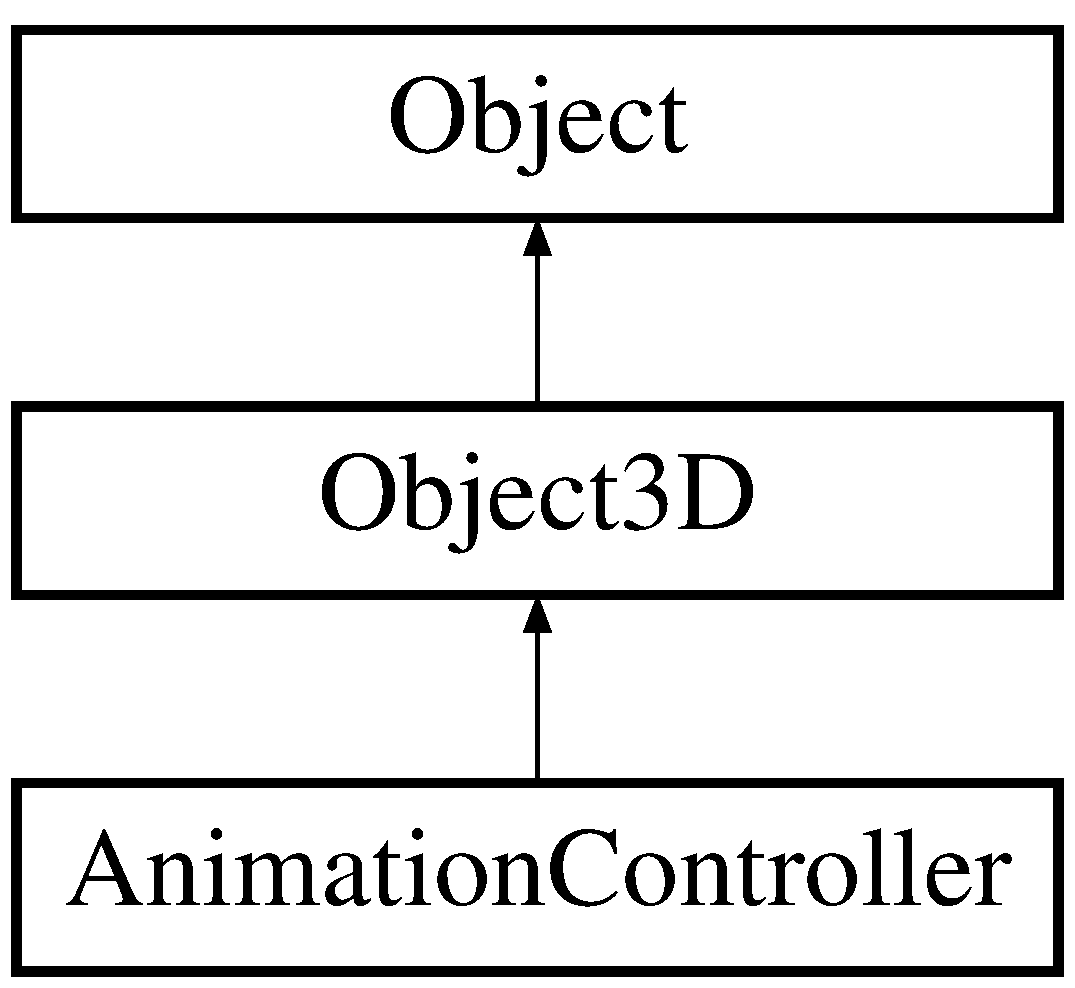
\includegraphics[height=3cm]{classm3g_1_1AnimationController}
\end{center}
\end{figure}
\subsection*{Classes}
\begin{CompactItemize}
\item 
struct \hyperlink{structm3g_1_1AnimationController_1_1ActiveInterval}{ActiveInterval}
\end{CompactItemize}
\subsection*{Public Member Functions}
\begin{CompactItemize}
\item 
\hyperlink{classm3g_1_1AnimationController_f2e8cb2c6c916983d0f87140c7b0c98e}{AnimationController} ()
\item 
virtual \hyperlink{classm3g_1_1AnimationController_346849d0f82278f30dda9f35f80e9dbe}{$\sim$AnimationController} ()
\item 
virtual \hyperlink{classm3g_1_1AnimationController}{AnimationController} $\ast$ \hyperlink{classm3g_1_1AnimationController_aab6521891038ced0961ecb78611646e}{duplicate} () const 
\item 
int \hyperlink{classm3g_1_1AnimationController_7caa95c7ed5a03844abe328feaae4911}{getActiveIntervalEnd} () const 
\item 
int \hyperlink{classm3g_1_1AnimationController_c66e837ae4152477eabdfcbe7fb21adb}{getActiveIntervalStart} () const 
\item 
float \hyperlink{classm3g_1_1AnimationController_dfdea73153cb34c26979575efda149e2}{getPosition} (int world\_\-time) const 
\item 
int \hyperlink{classm3g_1_1AnimationController_103e1bd81eba2cc90f31e7fdc4f3c601}{getRefWorldTime} () const 
\item 
float \hyperlink{classm3g_1_1AnimationController_4ab87c5df7c3eadd17b318a426773fcb}{getSpeed} () const 
\item 
float \hyperlink{classm3g_1_1AnimationController_a17d38dafd3d75c59f0609f037fbe5ae}{getWeight} () const 
\item 
void \hyperlink{classm3g_1_1AnimationController_a4cba877288d7a188477e0a756fd2f58}{setActiveInterval} (int start, int end)
\item 
void \hyperlink{classm3g_1_1AnimationController_da0d7a404b2a75ee182ca6351cf673d5}{setPosition} (float sequence\_\-time, int world\_\-time)
\item 
void \hyperlink{classm3g_1_1AnimationController_b32791d1a51df9ac8028792a841d06a6}{setSpeed} (float speed, int world\_\-time)
\item 
void \hyperlink{classm3g_1_1AnimationController_8859df4d5a61714012bf9e1240189aed}{setWeight} (float weight)
\item 
bool \hyperlink{classm3g_1_1AnimationController_8db30a5f125f5b22a1cde9e41d93c2f0}{isActiveInterval} (int world\_\-time) const 
\item 
virtual std::ostream \& \hyperlink{classm3g_1_1AnimationController_6fea17fa1532df3794f8cb39cb4f911f}{print} (std::ostream \&out) const 
\end{CompactItemize}


\subsection{Detailed Description}
Controls the position, speed and weight of an animation sequence. 

\subsection{Constructor \& Destructor Documentation}
\hypertarget{classm3g_1_1AnimationController_f2e8cb2c6c916983d0f87140c7b0c98e}{
\index{m3g::AnimationController@{m3g::AnimationController}!AnimationController@{AnimationController}}
\index{AnimationController@{AnimationController}!m3g::AnimationController@{m3g::AnimationController}}
\subsubsection[{AnimationController}]{\setlength{\rightskip}{0pt plus 5cm}{\bf AnimationController} ()}}
\label{classm3g_1_1AnimationController_f2e8cb2c6c916983d0f87140c7b0c98e}


Create a new \hyperlink{classm3g_1_1AnimationController}{AnimationController} object. \hypertarget{classm3g_1_1AnimationController_346849d0f82278f30dda9f35f80e9dbe}{
\index{m3g::AnimationController@{m3g::AnimationController}!$\sim$AnimationController@{$\sim$AnimationController}}
\index{$\sim$AnimationController@{$\sim$AnimationController}!m3g::AnimationController@{m3g::AnimationController}}
\subsubsection[{$\sim$AnimationController}]{\setlength{\rightskip}{0pt plus 5cm}$\sim${\bf AnimationController} ()\hspace{0.3cm}{\tt  \mbox{[}virtual\mbox{]}}}}
\label{classm3g_1_1AnimationController_346849d0f82278f30dda9f35f80e9dbe}


Destruct a \hyperlink{classm3g_1_1AnimationController}{AnimationController} object. 

\subsection{Member Function Documentation}
\hypertarget{classm3g_1_1AnimationController_aab6521891038ced0961ecb78611646e}{
\index{m3g::AnimationController@{m3g::AnimationController}!duplicate@{duplicate}}
\index{duplicate@{duplicate}!m3g::AnimationController@{m3g::AnimationController}}
\subsubsection[{duplicate}]{\setlength{\rightskip}{0pt plus 5cm}{\bf AnimationController} $\ast$ duplicate () const\hspace{0.3cm}{\tt  \mbox{[}virtual\mbox{]}}}}
\label{classm3g_1_1AnimationController_aab6521891038ced0961ecb78611646e}


Creates a duplicate of this \hyperlink{classm3g_1_1Object3D}{Object3D}. 

Reimplemented from \hyperlink{classm3g_1_1Object3D_a25110dac934f867b83b73ad4741a0f4}{Object3D}.\hypertarget{classm3g_1_1AnimationController_7caa95c7ed5a03844abe328feaae4911}{
\index{m3g::AnimationController@{m3g::AnimationController}!getActiveIntervalEnd@{getActiveIntervalEnd}}
\index{getActiveIntervalEnd@{getActiveIntervalEnd}!m3g::AnimationController@{m3g::AnimationController}}
\subsubsection[{getActiveIntervalEnd}]{\setlength{\rightskip}{0pt plus 5cm}int getActiveIntervalEnd () const}}
\label{classm3g_1_1AnimationController_7caa95c7ed5a03844abe328feaae4911}


Retrieve the ending time of the current active interval of this animation controller, in the world time units. \hypertarget{classm3g_1_1AnimationController_c66e837ae4152477eabdfcbe7fb21adb}{
\index{m3g::AnimationController@{m3g::AnimationController}!getActiveIntervalStart@{getActiveIntervalStart}}
\index{getActiveIntervalStart@{getActiveIntervalStart}!m3g::AnimationController@{m3g::AnimationController}}
\subsubsection[{getActiveIntervalStart}]{\setlength{\rightskip}{0pt plus 5cm}int getActiveIntervalStart () const}}
\label{classm3g_1_1AnimationController_c66e837ae4152477eabdfcbe7fb21adb}


Retrieve the starting time of the current active interval of this animation controller, in the world time units. \hypertarget{classm3g_1_1AnimationController_dfdea73153cb34c26979575efda149e2}{
\index{m3g::AnimationController@{m3g::AnimationController}!getPosition@{getPosition}}
\index{getPosition@{getPosition}!m3g::AnimationController@{m3g::AnimationController}}
\subsubsection[{getPosition}]{\setlength{\rightskip}{0pt plus 5cm}float getPosition (int {\em world\_\-time}) const}}
\label{classm3g_1_1AnimationController_dfdea73153cb34c26979575efda149e2}


Retrievews the sequence time that corresponds to the given world time. \hypertarget{classm3g_1_1AnimationController_103e1bd81eba2cc90f31e7fdc4f3c601}{
\index{m3g::AnimationController@{m3g::AnimationController}!getRefWorldTime@{getRefWorldTime}}
\index{getRefWorldTime@{getRefWorldTime}!m3g::AnimationController@{m3g::AnimationController}}
\subsubsection[{getRefWorldTime}]{\setlength{\rightskip}{0pt plus 5cm}int getRefWorldTime () const}}
\label{classm3g_1_1AnimationController_103e1bd81eba2cc90f31e7fdc4f3c601}


Returns the current feference world time. \hypertarget{classm3g_1_1AnimationController_4ab87c5df7c3eadd17b318a426773fcb}{
\index{m3g::AnimationController@{m3g::AnimationController}!getSpeed@{getSpeed}}
\index{getSpeed@{getSpeed}!m3g::AnimationController@{m3g::AnimationController}}
\subsubsection[{getSpeed}]{\setlength{\rightskip}{0pt plus 5cm}float getSpeed () const}}
\label{classm3g_1_1AnimationController_4ab87c5df7c3eadd17b318a426773fcb}


Retrieves the currently set playback speed of this animation controller. \hypertarget{classm3g_1_1AnimationController_a17d38dafd3d75c59f0609f037fbe5ae}{
\index{m3g::AnimationController@{m3g::AnimationController}!getWeight@{getWeight}}
\index{getWeight@{getWeight}!m3g::AnimationController@{m3g::AnimationController}}
\subsubsection[{getWeight}]{\setlength{\rightskip}{0pt plus 5cm}float getWeight () const}}
\label{classm3g_1_1AnimationController_a17d38dafd3d75c59f0609f037fbe5ae}


Retrieves the currently set blending weight for this animation controller. \hypertarget{classm3g_1_1AnimationController_8db30a5f125f5b22a1cde9e41d93c2f0}{
\index{m3g::AnimationController@{m3g::AnimationController}!isActiveInterval@{isActiveInterval}}
\index{isActiveInterval@{isActiveInterval}!m3g::AnimationController@{m3g::AnimationController}}
\subsubsection[{isActiveInterval}]{\setlength{\rightskip}{0pt plus 5cm}bool isActiveInterval (int {\em world\_\-time}) const}}
\label{classm3g_1_1AnimationController_8db30a5f125f5b22a1cde9e41d93c2f0}


query specified world\_\-time is in active interval, This is not under M3G spesification. @$^\wedge$Japanese 指定されたworld\_\-timeがアクティブ区間内だったらtrueを返すM3G非標準の関数. \hypertarget{classm3g_1_1AnimationController_6fea17fa1532df3794f8cb39cb4f911f}{
\index{m3g::AnimationController@{m3g::AnimationController}!print@{print}}
\index{print@{print}!m3g::AnimationController@{m3g::AnimationController}}
\subsubsection[{print}]{\setlength{\rightskip}{0pt plus 5cm}std::ostream \& print (std::ostream \& {\em out}) const\hspace{0.3cm}{\tt  \mbox{[}virtual\mbox{]}}}}
\label{classm3g_1_1AnimationController_6fea17fa1532df3794f8cb39cb4f911f}


Print out information of this class, for debug only. 

Reimplemented from \hyperlink{classm3g_1_1Object3D_6fea17fa1532df3794f8cb39cb4f911f}{Object3D}.\hypertarget{classm3g_1_1AnimationController_a4cba877288d7a188477e0a756fd2f58}{
\index{m3g::AnimationController@{m3g::AnimationController}!setActiveInterval@{setActiveInterval}}
\index{setActiveInterval@{setActiveInterval}!m3g::AnimationController@{m3g::AnimationController}}
\subsubsection[{setActiveInterval}]{\setlength{\rightskip}{0pt plus 5cm}void setActiveInterval (int {\em start}, \/  int {\em end})}}
\label{classm3g_1_1AnimationController_a4cba877288d7a188477e0a756fd2f58}


Sets the world time interval during which this animation controller is active. \hypertarget{classm3g_1_1AnimationController_da0d7a404b2a75ee182ca6351cf673d5}{
\index{m3g::AnimationController@{m3g::AnimationController}!setPosition@{setPosition}}
\index{setPosition@{setPosition}!m3g::AnimationController@{m3g::AnimationController}}
\subsubsection[{setPosition}]{\setlength{\rightskip}{0pt plus 5cm}void setPosition (float {\em sequence\_\-time}, \/  int {\em world\_\-time})}}
\label{classm3g_1_1AnimationController_da0d7a404b2a75ee182ca6351cf673d5}


Sets a new playback position, relative to world time. \hypertarget{classm3g_1_1AnimationController_b32791d1a51df9ac8028792a841d06a6}{
\index{m3g::AnimationController@{m3g::AnimationController}!setSpeed@{setSpeed}}
\index{setSpeed@{setSpeed}!m3g::AnimationController@{m3g::AnimationController}}
\subsubsection[{setSpeed}]{\setlength{\rightskip}{0pt plus 5cm}void setSpeed (float {\em speed}, \/  int {\em world\_\-time})}}
\label{classm3g_1_1AnimationController_b32791d1a51df9ac8028792a841d06a6}


Sets a new playback speed for this animation. \hypertarget{classm3g_1_1AnimationController_8859df4d5a61714012bf9e1240189aed}{
\index{m3g::AnimationController@{m3g::AnimationController}!setWeight@{setWeight}}
\index{setWeight@{setWeight}!m3g::AnimationController@{m3g::AnimationController}}
\subsubsection[{setWeight}]{\setlength{\rightskip}{0pt plus 5cm}void setWeight (float {\em weight})}}
\label{classm3g_1_1AnimationController_8859df4d5a61714012bf9e1240189aed}


Sets the blending weight for this animation controller. 

The documentation for this class was generated from the following files:\begin{CompactItemize}
\item 
/work/workspace.desktop-m3g/src/AnimationController.hpp\item 
/work/workspace.desktop-m3g/src/AnimationController.cpp\end{CompactItemize}

\hypertarget{classm3g_1_1AnimationTrack}{
\section{クラス AnimationTrack}
\label{classm3g_1_1AnimationTrack}\index{m3g::AnimationTrack@{m3g::AnimationTrack}}
}
{\tt \#include $<$AnimationTrack.hpp$>$}

AnimationTrackに対する継承グラフ:\begin{figure}[H]
\begin{center}
\leavevmode
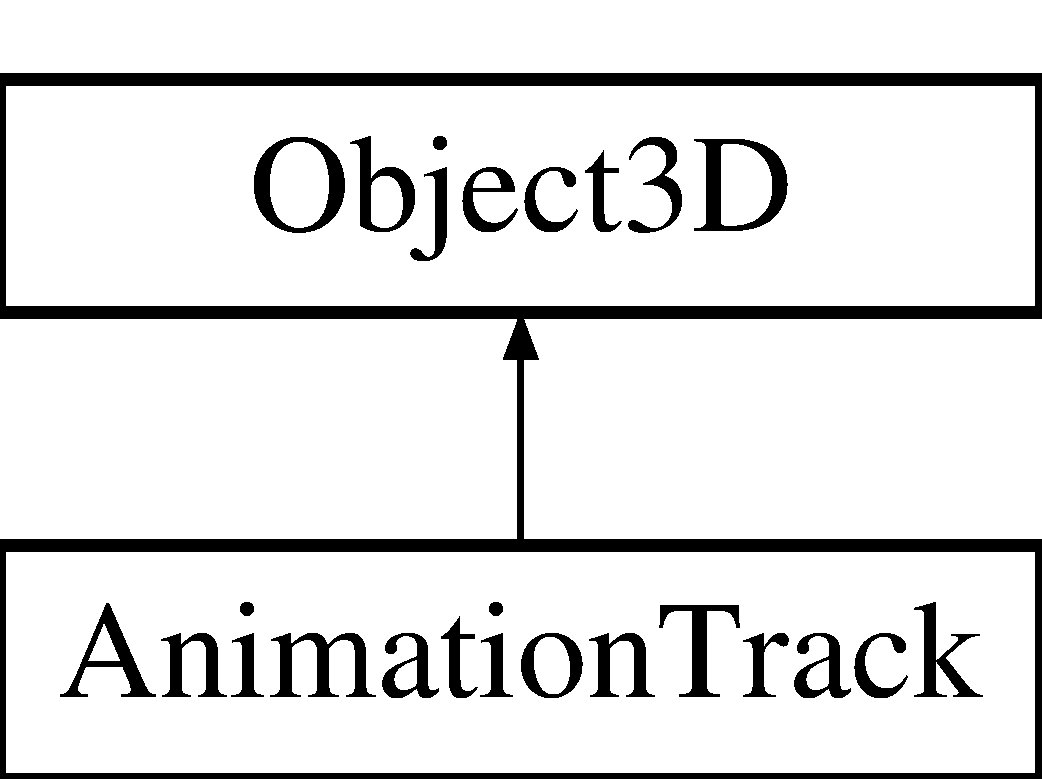
\includegraphics[height=3cm]{classm3g_1_1AnimationTrack}
\end{center}
\end{figure}
\subsection*{Public メソッド}
\begin{CompactItemize}
\item 
\hyperlink{classm3g_1_1AnimationTrack_e27012f60e982597d6e504c488e51106}{AnimationTrack} (\hyperlink{classm3g_1_1KeyframeSequence}{KeyframeSequence} $\ast$sequence, int property)
\item 
virtual \hyperlink{classm3g_1_1AnimationTrack_f7f1bc360c298d4a2f2436889159205c}{$\sim$AnimationTrack} ()
\item 
virtual \hyperlink{classm3g_1_1AnimationTrack}{AnimationTrack} $\ast$ \hyperlink{classm3g_1_1AnimationTrack_e19aae30ee68ef05afd74ec9c19cf7d1}{duplicate} () const 
\item 
\hyperlink{classm3g_1_1AnimationController}{AnimationController} $\ast$ \hyperlink{classm3g_1_1AnimationTrack_3a54e89528127de5b4d0a48a2045a91c}{getController} () const 
\item 
\hyperlink{classm3g_1_1KeyframeSequence}{KeyframeSequence} $\ast$ \hyperlink{classm3g_1_1AnimationTrack_e83c81771a8329e1e5f978f228c0b308}{getKeyframeSequence} () const 
\item 
int \hyperlink{classm3g_1_1AnimationTrack_143de0bf90b434f1487caae5b0b66bbf}{getTargetProperty} () const 
\item 
void \hyperlink{classm3g_1_1AnimationTrack_639279dfdc74095fcb28d0c25aeec6df}{setController} (\hyperlink{classm3g_1_1AnimationController}{AnimationController} $\ast$controller)
\item 
virtual std::ostream \& \hyperlink{classm3g_1_1AnimationTrack_6fea17fa1532df3794f8cb39cb4f911f}{print} (std::ostream \&out) const 
\end{CompactItemize}
\subsection*{Static Public 変数}
\begin{CompactItemize}
\item 
static const int \hyperlink{classm3g_1_1AnimationTrack_417581fcde4067111f47320edb2aa378}{ALPHA} = 256
\item 
static const int \hyperlink{classm3g_1_1AnimationTrack_71b6e9c23b95f8011da4565f4a12f677}{AMBIENT\_\-COLOR} = 257
\item 
static const int \hyperlink{classm3g_1_1AnimationTrack_a6d8034c897057de595a4511a4e7a837}{COLOR} = 258
\item 
static const int \hyperlink{classm3g_1_1AnimationTrack_91fa562078e577c24d06faf8391b34fe}{CROP} = 259
\item 
static const int \hyperlink{classm3g_1_1AnimationTrack_7d0fe4463930d4a4b24fc47660561899}{DENSITY} = 260
\item 
static const int \hyperlink{classm3g_1_1AnimationTrack_9631242a611cf95d697c25064dba7c4f}{DIFFUSE\_\-COLOR} = 261
\item 
static const int \hyperlink{classm3g_1_1AnimationTrack_893461d45d084e5db05b159068f945d0}{EMISSIVE\_\-COLOR} = 262
\item 
static const int \hyperlink{classm3g_1_1AnimationTrack_86457ec0a2799f1f2d7ea8173a644de8}{FAR\_\-DISTANCE} = 263
\item 
static const int \hyperlink{classm3g_1_1AnimationTrack_94c1c1d2f7d48b52e3c2bcd332ed3937}{FIELD\_\-OF\_\-VIEW} = 264
\item 
static const int \hyperlink{classm3g_1_1AnimationTrack_369fe8830f39fe4aec819a371a6c9904}{INTENSITY} = 265
\item 
static const int \hyperlink{classm3g_1_1AnimationTrack_d75f3e3033e268d0a74f9533cfa9b9d6}{MORPH\_\-WEIGHTS} = 266
\item 
static const int \hyperlink{classm3g_1_1AnimationTrack_74f49e3b52778aff378dac012e59cdb2}{NEAR\_\-DISTANCE} = 267
\item 
static const int \hyperlink{classm3g_1_1AnimationTrack_c7fe423a6a639520b0b3d1c1e663784b}{ORIENTATION} = 268
\item 
static const int \hyperlink{classm3g_1_1AnimationTrack_87fcd8136941a05a8a95c61e499692e0}{PICKABILITY} = 269
\item 
static const int \hyperlink{classm3g_1_1AnimationTrack_8334f0c0c56b96debb10231b86050ead}{SCALE} = 270
\item 
static const int \hyperlink{classm3g_1_1AnimationTrack_f0b58ddb4173a8d2f5a730dab30e6c6f}{SHININESS} = 271
\item 
static const int \hyperlink{classm3g_1_1AnimationTrack_a0119030157ee8a5ef4f8ce88771447b}{SPECULAR\_\-COLOR} = 272
\item 
static const int \hyperlink{classm3g_1_1AnimationTrack_c1d6b5313ef35ef100889ca885901db2}{SPOT\_\-ANGLE} = 273
\item 
static const int \hyperlink{classm3g_1_1AnimationTrack_90c55bd356e55166244416c6f758ea94}{SPOT\_\-EXPONENT} = 274
\item 
static const int \hyperlink{classm3g_1_1AnimationTrack_a691826dccd8c22144e61216de4f680c}{TRANSLATION} = 275
\item 
static const int \hyperlink{classm3g_1_1AnimationTrack_f248c44b5d4962472c6533cdeffc6fe9}{VISIBILITY} = 276
\end{CompactItemize}


\subsection{説明}
アニメーションコントローラーやアニメーション可能なプロパティを キーフレームシーケンスに関連づける. 

\subsection{コンストラクタとデストラクタ}
\hypertarget{classm3g_1_1AnimationTrack_e27012f60e982597d6e504c488e51106}{
\index{m3g::AnimationTrack@{m3g::AnimationTrack}!AnimationTrack@{AnimationTrack}}
\index{AnimationTrack@{AnimationTrack}!m3g::AnimationTrack@{m3g::AnimationTrack}}
\subsubsection[{AnimationTrack}]{\setlength{\rightskip}{0pt plus 5cm}{\bf AnimationTrack} ({\bf KeyframeSequence} $\ast$ {\em sequence}, \/  int {\em property})}}
\label{classm3g_1_1AnimationTrack_e27012f60e982597d6e504c488e51106}


指定されたプロパティのキーフレームシーケンスを持つ アニメーショントラックを作成する. \hypertarget{classm3g_1_1AnimationTrack_f7f1bc360c298d4a2f2436889159205c}{
\index{m3g::AnimationTrack@{m3g::AnimationTrack}!$\sim$AnimationTrack@{$\sim$AnimationTrack}}
\index{$\sim$AnimationTrack@{$\sim$AnimationTrack}!m3g::AnimationTrack@{m3g::AnimationTrack}}
\subsubsection[{$\sim$AnimationTrack}]{\setlength{\rightskip}{0pt plus 5cm}$\sim${\bf AnimationTrack} ()\hspace{0.3cm}{\tt  \mbox{[}virtual\mbox{]}}}}
\label{classm3g_1_1AnimationTrack_f7f1bc360c298d4a2f2436889159205c}


AnimationTrackクラスのデストラクタ. 

\subsection{関数}
\hypertarget{classm3g_1_1AnimationTrack_e19aae30ee68ef05afd74ec9c19cf7d1}{
\index{m3g::AnimationTrack@{m3g::AnimationTrack}!duplicate@{duplicate}}
\index{duplicate@{duplicate}!m3g::AnimationTrack@{m3g::AnimationTrack}}
\subsubsection[{duplicate}]{\setlength{\rightskip}{0pt plus 5cm}{\bf AnimationTrack} $\ast$ duplicate () const\hspace{0.3cm}{\tt  \mbox{[}virtual\mbox{]}}}}
\label{classm3g_1_1AnimationTrack_e19aae30ee68ef05afd74ec9c19cf7d1}


このオブジェクトの複製の作成. 

\hyperlink{classm3g_1_1Object3D_a25110dac934f867b83b73ad4741a0f4}{Object3D}を再定義しています。\hypertarget{classm3g_1_1AnimationTrack_3a54e89528127de5b4d0a48a2045a91c}{
\index{m3g::AnimationTrack@{m3g::AnimationTrack}!getController@{getController}}
\index{getController@{getController}!m3g::AnimationTrack@{m3g::AnimationTrack}}
\subsubsection[{getController}]{\setlength{\rightskip}{0pt plus 5cm}{\bf AnimationController} $\ast$ getController () const}}
\label{classm3g_1_1AnimationTrack_3a54e89528127de5b4d0a48a2045a91c}


このアニメーショントラックを制御するアニメーションコントローラーを取得する. \hypertarget{classm3g_1_1AnimationTrack_e83c81771a8329e1e5f978f228c0b308}{
\index{m3g::AnimationTrack@{m3g::AnimationTrack}!getKeyframeSequence@{getKeyframeSequence}}
\index{getKeyframeSequence@{getKeyframeSequence}!m3g::AnimationTrack@{m3g::AnimationTrack}}
\subsubsection[{getKeyframeSequence}]{\setlength{\rightskip}{0pt plus 5cm}{\bf KeyframeSequence} $\ast$ getKeyframeSequence () const}}
\label{classm3g_1_1AnimationTrack_e83c81771a8329e1e5f978f228c0b308}


このアニメーショントラック用のキーフレームの値を持つキーフレームシーケンスを取得する. \hypertarget{classm3g_1_1AnimationTrack_143de0bf90b434f1487caae5b0b66bbf}{
\index{m3g::AnimationTrack@{m3g::AnimationTrack}!getTargetProperty@{getTargetProperty}}
\index{getTargetProperty@{getTargetProperty}!m3g::AnimationTrack@{m3g::AnimationTrack}}
\subsubsection[{getTargetProperty}]{\setlength{\rightskip}{0pt plus 5cm}int getTargetProperty () const}}
\label{classm3g_1_1AnimationTrack_143de0bf90b434f1487caae5b0b66bbf}


このアニメーショントラックによるターゲットプロパティを取得する. \hypertarget{classm3g_1_1AnimationTrack_6fea17fa1532df3794f8cb39cb4f911f}{
\index{m3g::AnimationTrack@{m3g::AnimationTrack}!print@{print}}
\index{print@{print}!m3g::AnimationTrack@{m3g::AnimationTrack}}
\subsubsection[{print}]{\setlength{\rightskip}{0pt plus 5cm}std::ostream \& print (std::ostream \& {\em out}) const\hspace{0.3cm}{\tt  \mbox{[}virtual\mbox{]}}}}
\label{classm3g_1_1AnimationTrack_6fea17fa1532df3794f8cb39cb4f911f}


このAnimationTrackクラスの情報を表示する。デバッグ用. 

\hyperlink{classm3g_1_1Object3D_6fea17fa1532df3794f8cb39cb4f911f}{Object3D}を再定義しています。\hypertarget{classm3g_1_1AnimationTrack_639279dfdc74095fcb28d0c25aeec6df}{
\index{m3g::AnimationTrack@{m3g::AnimationTrack}!setController@{setController}}
\index{setController@{setController}!m3g::AnimationTrack@{m3g::AnimationTrack}}
\subsubsection[{setController}]{\setlength{\rightskip}{0pt plus 5cm}void setController ({\bf AnimationController} $\ast$ {\em controller})}}
\label{classm3g_1_1AnimationTrack_639279dfdc74095fcb28d0c25aeec6df}


このアニメーショントラックを制御するアニメーションコントローラーを設定する. 

\subsection{変数}
\hypertarget{classm3g_1_1AnimationTrack_417581fcde4067111f47320edb2aa378}{
\index{m3g::AnimationTrack@{m3g::AnimationTrack}!ALPHA@{ALPHA}}
\index{ALPHA@{ALPHA}!m3g::AnimationTrack@{m3g::AnimationTrack}}
\subsubsection[{ALPHA}]{\setlength{\rightskip}{0pt plus 5cm}const int {\bf ALPHA} = 256\hspace{0.3cm}{\tt  \mbox{[}static\mbox{]}}}}
\label{classm3g_1_1AnimationTrack_417581fcde4067111f47320edb2aa378}


ノードのα値や背景色、マテリアルの拡散カラー係数、 頂点バッファーのデフォルト色をアニメーションターゲットに指定する定数. \hypertarget{classm3g_1_1AnimationTrack_71b6e9c23b95f8011da4565f4a12f677}{
\index{m3g::AnimationTrack@{m3g::AnimationTrack}!AMBIENT\_\-COLOR@{AMBIENT\_\-COLOR}}
\index{AMBIENT\_\-COLOR@{AMBIENT\_\-COLOR}!m3g::AnimationTrack@{m3g::AnimationTrack}}
\subsubsection[{AMBIENT\_\-COLOR}]{\setlength{\rightskip}{0pt plus 5cm}const int {\bf AMBIENT\_\-COLOR} = 257\hspace{0.3cm}{\tt  \mbox{[}static\mbox{]}}}}
\label{classm3g_1_1AnimationTrack_71b6e9c23b95f8011da4565f4a12f677}


マテリアルの環境光係数をアニメーションターゲットに指定する定数. \hypertarget{classm3g_1_1AnimationTrack_a6d8034c897057de595a4511a4e7a837}{
\index{m3g::AnimationTrack@{m3g::AnimationTrack}!COLOR@{COLOR}}
\index{COLOR@{COLOR}!m3g::AnimationTrack@{m3g::AnimationTrack}}
\subsubsection[{COLOR}]{\setlength{\rightskip}{0pt plus 5cm}const int {\bf COLOR} = 258\hspace{0.3cm}{\tt  \mbox{[}static\mbox{]}}}}
\label{classm3g_1_1AnimationTrack_a6d8034c897057de595a4511a4e7a837}


ライト、バックグラウンド、フォグ、テクスチャーのブレンド色、 頂点バッファーのデフォルト色をアニメーションターゲットに指定する定数. \hypertarget{classm3g_1_1AnimationTrack_91fa562078e577c24d06faf8391b34fe}{
\index{m3g::AnimationTrack@{m3g::AnimationTrack}!CROP@{CROP}}
\index{CROP@{CROP}!m3g::AnimationTrack@{m3g::AnimationTrack}}
\subsubsection[{CROP}]{\setlength{\rightskip}{0pt plus 5cm}const int {\bf CROP} = 259\hspace{0.3cm}{\tt  \mbox{[}static\mbox{]}}}}
\label{classm3g_1_1AnimationTrack_91fa562078e577c24d06faf8391b34fe}


スプライト3Dや背景のクロップパラメーターをアニメーションターゲットに 指定する定数. \hypertarget{classm3g_1_1AnimationTrack_7d0fe4463930d4a4b24fc47660561899}{
\index{m3g::AnimationTrack@{m3g::AnimationTrack}!DENSITY@{DENSITY}}
\index{DENSITY@{DENSITY}!m3g::AnimationTrack@{m3g::AnimationTrack}}
\subsubsection[{DENSITY}]{\setlength{\rightskip}{0pt plus 5cm}const int {\bf DENSITY} = 260\hspace{0.3cm}{\tt  \mbox{[}static\mbox{]}}}}
\label{classm3g_1_1AnimationTrack_7d0fe4463930d4a4b24fc47660561899}


フォグのフォグ密度をアニメーションターゲットに指定する定数. \hypertarget{classm3g_1_1AnimationTrack_9631242a611cf95d697c25064dba7c4f}{
\index{m3g::AnimationTrack@{m3g::AnimationTrack}!DIFFUSE\_\-COLOR@{DIFFUSE\_\-COLOR}}
\index{DIFFUSE\_\-COLOR@{DIFFUSE\_\-COLOR}!m3g::AnimationTrack@{m3g::AnimationTrack}}
\subsubsection[{DIFFUSE\_\-COLOR}]{\setlength{\rightskip}{0pt plus 5cm}const int {\bf DIFFUSE\_\-COLOR} = 261\hspace{0.3cm}{\tt  \mbox{[}static\mbox{]}}}}
\label{classm3g_1_1AnimationTrack_9631242a611cf95d697c25064dba7c4f}


マテリアルの拡散カラー係数をアニメーションターゲットに指定する定数. \hypertarget{classm3g_1_1AnimationTrack_893461d45d084e5db05b159068f945d0}{
\index{m3g::AnimationTrack@{m3g::AnimationTrack}!EMISSIVE\_\-COLOR@{EMISSIVE\_\-COLOR}}
\index{EMISSIVE\_\-COLOR@{EMISSIVE\_\-COLOR}!m3g::AnimationTrack@{m3g::AnimationTrack}}
\subsubsection[{EMISSIVE\_\-COLOR}]{\setlength{\rightskip}{0pt plus 5cm}const int {\bf EMISSIVE\_\-COLOR} = 262\hspace{0.3cm}{\tt  \mbox{[}static\mbox{]}}}}
\label{classm3g_1_1AnimationTrack_893461d45d084e5db05b159068f945d0}


マテリアルの事故発光カラー係数をアニメーションターゲットに指定する定数. \hypertarget{classm3g_1_1AnimationTrack_86457ec0a2799f1f2d7ea8173a644de8}{
\index{m3g::AnimationTrack@{m3g::AnimationTrack}!FAR\_\-DISTANCE@{FAR\_\-DISTANCE}}
\index{FAR\_\-DISTANCE@{FAR\_\-DISTANCE}!m3g::AnimationTrack@{m3g::AnimationTrack}}
\subsubsection[{FAR\_\-DISTANCE}]{\setlength{\rightskip}{0pt plus 5cm}const int {\bf FAR\_\-DISTANCE} = 263\hspace{0.3cm}{\tt  \mbox{[}static\mbox{]}}}}
\label{classm3g_1_1AnimationTrack_86457ec0a2799f1f2d7ea8173a644de8}


カメラもしくはフォグのファー距離をアニメーションターゲットに指定する定数. \hypertarget{classm3g_1_1AnimationTrack_94c1c1d2f7d48b52e3c2bcd332ed3937}{
\index{m3g::AnimationTrack@{m3g::AnimationTrack}!FIELD\_\-OF\_\-VIEW@{FIELD\_\-OF\_\-VIEW}}
\index{FIELD\_\-OF\_\-VIEW@{FIELD\_\-OF\_\-VIEW}!m3g::AnimationTrack@{m3g::AnimationTrack}}
\subsubsection[{FIELD\_\-OF\_\-VIEW}]{\setlength{\rightskip}{0pt plus 5cm}const int {\bf FIELD\_\-OF\_\-VIEW} = 264\hspace{0.3cm}{\tt  \mbox{[}static\mbox{]}}}}
\label{classm3g_1_1AnimationTrack_94c1c1d2f7d48b52e3c2bcd332ed3937}


カメラの視野角をアニメーションターゲットに指定する定数. \hypertarget{classm3g_1_1AnimationTrack_369fe8830f39fe4aec819a371a6c9904}{
\index{m3g::AnimationTrack@{m3g::AnimationTrack}!INTENSITY@{INTENSITY}}
\index{INTENSITY@{INTENSITY}!m3g::AnimationTrack@{m3g::AnimationTrack}}
\subsubsection[{INTENSITY}]{\setlength{\rightskip}{0pt plus 5cm}const int {\bf INTENSITY} = 265\hspace{0.3cm}{\tt  \mbox{[}static\mbox{]}}}}
\label{classm3g_1_1AnimationTrack_369fe8830f39fe4aec819a371a6c9904}


ライトの強度をアニメーションターゲットに指定する定数. \hypertarget{classm3g_1_1AnimationTrack_d75f3e3033e268d0a74f9533cfa9b9d6}{
\index{m3g::AnimationTrack@{m3g::AnimationTrack}!MORPH\_\-WEIGHTS@{MORPH\_\-WEIGHTS}}
\index{MORPH\_\-WEIGHTS@{MORPH\_\-WEIGHTS}!m3g::AnimationTrack@{m3g::AnimationTrack}}
\subsubsection[{MORPH\_\-WEIGHTS}]{\setlength{\rightskip}{0pt plus 5cm}const int {\bf MORPH\_\-WEIGHTS} = 266\hspace{0.3cm}{\tt  \mbox{[}static\mbox{]}}}}
\label{classm3g_1_1AnimationTrack_d75f3e3033e268d0a74f9533cfa9b9d6}


モーフィングメッシュのモーフターゲットウェイトをアニメーションターゲットに指定する定数. \hypertarget{classm3g_1_1AnimationTrack_74f49e3b52778aff378dac012e59cdb2}{
\index{m3g::AnimationTrack@{m3g::AnimationTrack}!NEAR\_\-DISTANCE@{NEAR\_\-DISTANCE}}
\index{NEAR\_\-DISTANCE@{NEAR\_\-DISTANCE}!m3g::AnimationTrack@{m3g::AnimationTrack}}
\subsubsection[{NEAR\_\-DISTANCE}]{\setlength{\rightskip}{0pt plus 5cm}const int {\bf NEAR\_\-DISTANCE} = 267\hspace{0.3cm}{\tt  \mbox{[}static\mbox{]}}}}
\label{classm3g_1_1AnimationTrack_74f49e3b52778aff378dac012e59cdb2}


カメラもしくはフォグのニア距離をアニメーションターゲットに指定する定数. \hypertarget{classm3g_1_1AnimationTrack_c7fe423a6a639520b0b3d1c1e663784b}{
\index{m3g::AnimationTrack@{m3g::AnimationTrack}!ORIENTATION@{ORIENTATION}}
\index{ORIENTATION@{ORIENTATION}!m3g::AnimationTrack@{m3g::AnimationTrack}}
\subsubsection[{ORIENTATION}]{\setlength{\rightskip}{0pt plus 5cm}const int {\bf ORIENTATION} = 268\hspace{0.3cm}{\tt  \mbox{[}static\mbox{]}}}}
\label{classm3g_1_1AnimationTrack_c7fe423a6a639520b0b3d1c1e663784b}


トランスフォーム可能なオブジェクトの回転成分をアニメーションターゲットに 指定する定数. \hypertarget{classm3g_1_1AnimationTrack_87fcd8136941a05a8a95c61e499692e0}{
\index{m3g::AnimationTrack@{m3g::AnimationTrack}!PICKABILITY@{PICKABILITY}}
\index{PICKABILITY@{PICKABILITY}!m3g::AnimationTrack@{m3g::AnimationTrack}}
\subsubsection[{PICKABILITY}]{\setlength{\rightskip}{0pt plus 5cm}const int {\bf PICKABILITY} = 269\hspace{0.3cm}{\tt  \mbox{[}static\mbox{]}}}}
\label{classm3g_1_1AnimationTrack_87fcd8136941a05a8a95c61e499692e0}


ノードのピッキング可能フラグをアニメーションターゲットに指定する定数. \hypertarget{classm3g_1_1AnimationTrack_8334f0c0c56b96debb10231b86050ead}{
\index{m3g::AnimationTrack@{m3g::AnimationTrack}!SCALE@{SCALE}}
\index{SCALE@{SCALE}!m3g::AnimationTrack@{m3g::AnimationTrack}}
\subsubsection[{SCALE}]{\setlength{\rightskip}{0pt plus 5cm}const int {\bf SCALE} = 270\hspace{0.3cm}{\tt  \mbox{[}static\mbox{]}}}}
\label{classm3g_1_1AnimationTrack_8334f0c0c56b96debb10231b86050ead}


トランスフォーム可能なオブジェクトのスケール成分を アニメーションターゲットに指定する定数. \hypertarget{classm3g_1_1AnimationTrack_f0b58ddb4173a8d2f5a730dab30e6c6f}{
\index{m3g::AnimationTrack@{m3g::AnimationTrack}!SHININESS@{SHININESS}}
\index{SHININESS@{SHININESS}!m3g::AnimationTrack@{m3g::AnimationTrack}}
\subsubsection[{SHININESS}]{\setlength{\rightskip}{0pt plus 5cm}const int {\bf SHININESS} = 271\hspace{0.3cm}{\tt  \mbox{[}static\mbox{]}}}}
\label{classm3g_1_1AnimationTrack_f0b58ddb4173a8d2f5a730dab30e6c6f}


マテリアルのshininess成分をアニメーションターゲットに指定する定数. \hypertarget{classm3g_1_1AnimationTrack_a0119030157ee8a5ef4f8ce88771447b}{
\index{m3g::AnimationTrack@{m3g::AnimationTrack}!SPECULAR\_\-COLOR@{SPECULAR\_\-COLOR}}
\index{SPECULAR\_\-COLOR@{SPECULAR\_\-COLOR}!m3g::AnimationTrack@{m3g::AnimationTrack}}
\subsubsection[{SPECULAR\_\-COLOR}]{\setlength{\rightskip}{0pt plus 5cm}const int {\bf SPECULAR\_\-COLOR} = 272\hspace{0.3cm}{\tt  \mbox{[}static\mbox{]}}}}
\label{classm3g_1_1AnimationTrack_a0119030157ee8a5ef4f8ce88771447b}


マテリアルの鏡面カラー係数をアニメーションターゲットに指定する定数. \hypertarget{classm3g_1_1AnimationTrack_c1d6b5313ef35ef100889ca885901db2}{
\index{m3g::AnimationTrack@{m3g::AnimationTrack}!SPOT\_\-ANGLE@{SPOT\_\-ANGLE}}
\index{SPOT\_\-ANGLE@{SPOT\_\-ANGLE}!m3g::AnimationTrack@{m3g::AnimationTrack}}
\subsubsection[{SPOT\_\-ANGLE}]{\setlength{\rightskip}{0pt plus 5cm}const int {\bf SPOT\_\-ANGLE} = 273\hspace{0.3cm}{\tt  \mbox{[}static\mbox{]}}}}
\label{classm3g_1_1AnimationTrack_c1d6b5313ef35ef100889ca885901db2}


ライトのスポット角度をアニメーションターゲットに指定する定数. \hypertarget{classm3g_1_1AnimationTrack_90c55bd356e55166244416c6f758ea94}{
\index{m3g::AnimationTrack@{m3g::AnimationTrack}!SPOT\_\-EXPONENT@{SPOT\_\-EXPONENT}}
\index{SPOT\_\-EXPONENT@{SPOT\_\-EXPONENT}!m3g::AnimationTrack@{m3g::AnimationTrack}}
\subsubsection[{SPOT\_\-EXPONENT}]{\setlength{\rightskip}{0pt plus 5cm}const int {\bf SPOT\_\-EXPONENT} = 274\hspace{0.3cm}{\tt  \mbox{[}static\mbox{]}}}}
\label{classm3g_1_1AnimationTrack_90c55bd356e55166244416c6f758ea94}


ライトのスポット指数係数をアニメーションターゲットに指定する定数. \hypertarget{classm3g_1_1AnimationTrack_a691826dccd8c22144e61216de4f680c}{
\index{m3g::AnimationTrack@{m3g::AnimationTrack}!TRANSLATION@{TRANSLATION}}
\index{TRANSLATION@{TRANSLATION}!m3g::AnimationTrack@{m3g::AnimationTrack}}
\subsubsection[{TRANSLATION}]{\setlength{\rightskip}{0pt plus 5cm}const int {\bf TRANSLATION} = 275\hspace{0.3cm}{\tt  \mbox{[}static\mbox{]}}}}
\label{classm3g_1_1AnimationTrack_a691826dccd8c22144e61216de4f680c}


トランスフォーム可能なオブジェクトの平行移動成分を アニメーションターゲットに指定する定数. \hypertarget{classm3g_1_1AnimationTrack_f248c44b5d4962472c6533cdeffc6fe9}{
\index{m3g::AnimationTrack@{m3g::AnimationTrack}!VISIBILITY@{VISIBILITY}}
\index{VISIBILITY@{VISIBILITY}!m3g::AnimationTrack@{m3g::AnimationTrack}}
\subsubsection[{VISIBILITY}]{\setlength{\rightskip}{0pt plus 5cm}const int {\bf VISIBILITY} = 276\hspace{0.3cm}{\tt  \mbox{[}static\mbox{]}}}}
\label{classm3g_1_1AnimationTrack_f248c44b5d4962472c6533cdeffc6fe9}


ノードのレンダリングフラグをアニメーションターゲットに指定する定数. 

このクラスの説明は次のファイルから生成されました:\begin{CompactItemize}
\item 
/work/workspace.desktop-m3g/src/AnimationTrack.hpp\item 
/work/workspace.desktop-m3g/src/AnimationTrack.cpp\end{CompactItemize}

\hypertarget{classm3g_1_1Appearance}{
\section{Appearance Class Reference}
\label{classm3g_1_1Appearance}\index{m3g::Appearance@{m3g::Appearance}}
}
{\tt \#include $<$Appearance.hpp$>$}

Inheritance diagram for Appearance::\begin{figure}[H]
\begin{center}
\leavevmode
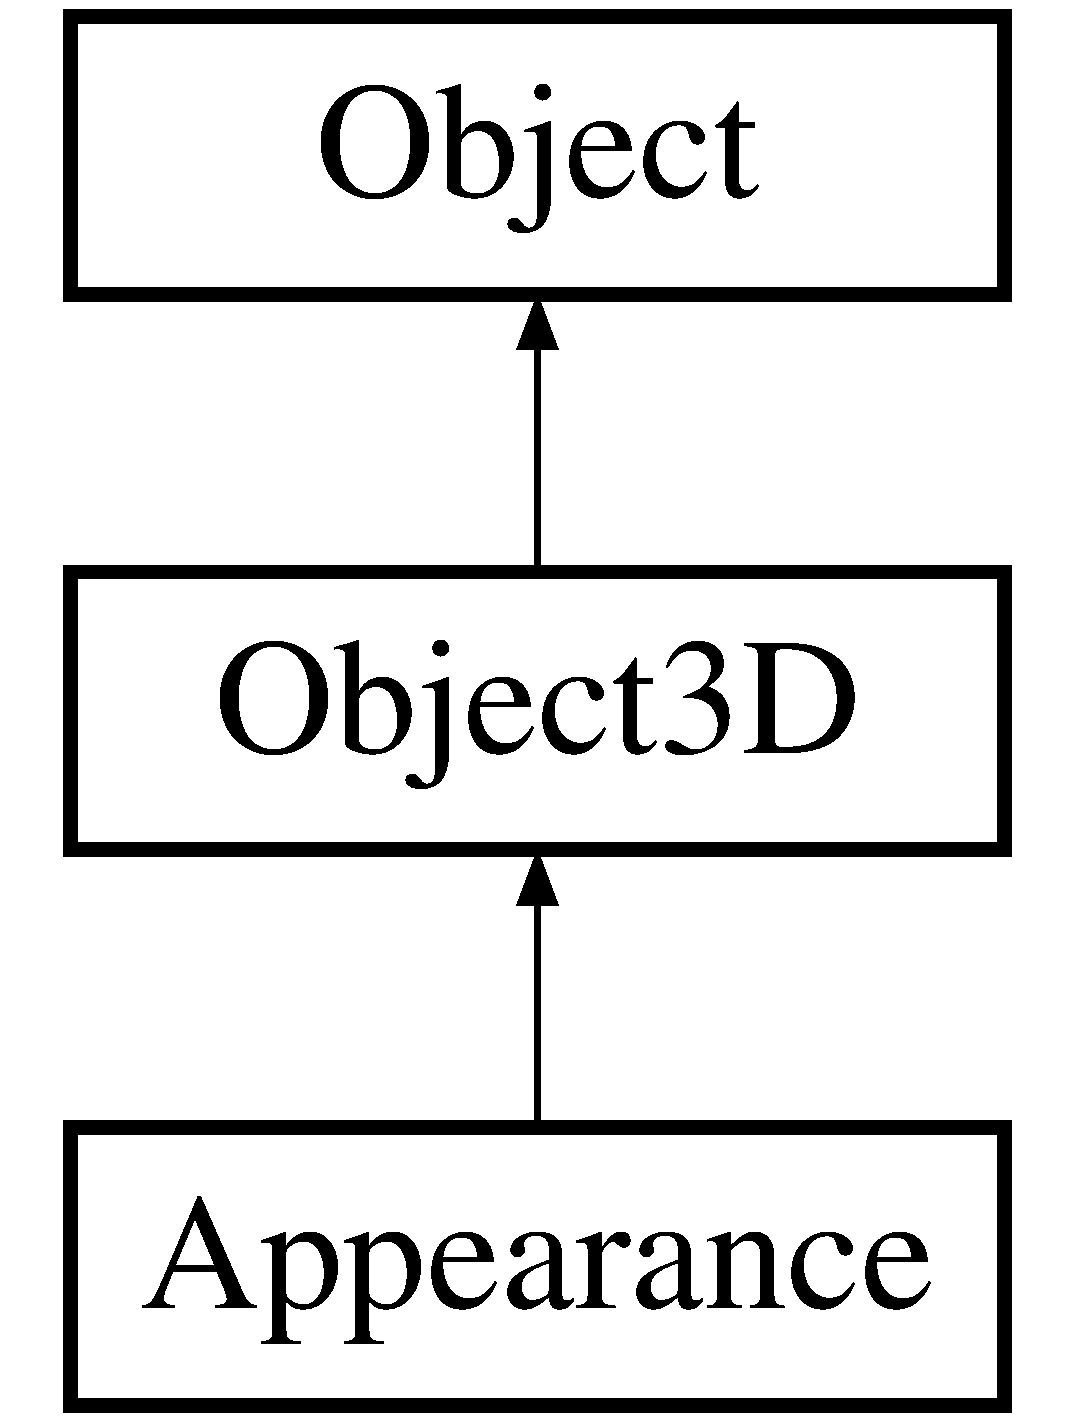
\includegraphics[height=2cm]{classm3g_1_1Appearance}
\end{center}
\end{figure}
\subsection*{Public Member Functions}
\begin{CompactItemize}
\item 
\hyperlink{classm3g_1_1Appearance_2e594c7b96cb5cfad839a98b57f5d42f}{Appearance} ()
\item 
virtual \hyperlink{classm3g_1_1Appearance_c05c93d7a0f286cb9471b6c667ffeee1}{$\sim$Appearance} ()
\item 
virtual int \hyperlink{classm3g_1_1Appearance_8aad1ceab4c2a03609c8a42324ce484d}{animate} (int world\_\-time)
\item 
\hyperlink{classm3g_1_1CompositingMode}{CompositingMode} $\ast$ \hyperlink{classm3g_1_1Appearance_e4045934febb56891c15e14486b239a8}{getCompositingMode} () const 
\item 
\hyperlink{classm3g_1_1Fog}{Fog} $\ast$ \hyperlink{classm3g_1_1Appearance_93143a921b998ff69576147a59eb44d4}{getFog} () const 
\item 
int \hyperlink{classm3g_1_1Appearance_df831e0e0ebf9d7e997150e497e6a6cf}{getLayer} () const 
\item 
\hypertarget{classm3g_1_1Appearance_a412c7074ed5d51f6b8b6fd89275c405}{
\hyperlink{classm3g_1_1Material}{Material} $\ast$ \textbf{getMaterial} () const }
\label{classm3g_1_1Appearance_a412c7074ed5d51f6b8b6fd89275c405}

\item 
PolygonMode $\ast$ \hyperlink{classm3g_1_1Appearance_dd3ddcefcd18339150d281b155602886}{getPolygonMode} () const 
\item 
\hypertarget{classm3g_1_1Appearance_987cc21bd78d0e4e664da717479bdd57}{
\hyperlink{classm3g_1_1Texture2D}{Texture2D} $\ast$ \textbf{getTexture} (int index) const }
\label{classm3g_1_1Appearance_987cc21bd78d0e4e664da717479bdd57}

\item 
void \hyperlink{classm3g_1_1Appearance_b4dbfc0232132aeb0a7b7c5eaade82e1}{setCompositingMode} (\hyperlink{classm3g_1_1CompositingMode}{CompositingMode} $\ast$compositingMode)
\item 
void \hyperlink{classm3g_1_1Appearance_bc1a612006d6b4c3d443ff6ab542c788}{setFog} (\hyperlink{classm3g_1_1Fog}{Fog} $\ast$fog)
\item 
void \hyperlink{classm3g_1_1Appearance_fbd2fbd594c8ee140b028f505631f682}{setLayer} (int layer)
\item 
\hypertarget{classm3g_1_1Appearance_1dfd1a55fa3cc625719dab8e95c8a2de}{
void \textbf{setMaterial} (\hyperlink{classm3g_1_1Material}{Material} $\ast$material)}
\label{classm3g_1_1Appearance_1dfd1a55fa3cc625719dab8e95c8a2de}

\item 
void \hyperlink{classm3g_1_1Appearance_cc21fac7868e2ad37e689ac642db1aae}{setPolygonMode} (PolygonMode $\ast$polygonMode)
\item 
void \hyperlink{classm3g_1_1Appearance_493e54b1c7ab839b9e76b28e0629cf6a}{setTexture} (int index, \hyperlink{classm3g_1_1Texture2D}{Texture2D} $\ast$texture)
\item 
virtual std::ostream \& \hyperlink{classm3g_1_1Appearance_6fea17fa1532df3794f8cb39cb4f911f}{print} (std::ostream \&out) const 
\end{CompactItemize}
\subsection*{Protected Member Functions}
\begin{CompactItemize}
\item 
virtual void \hyperlink{classm3g_1_1Appearance_4dadb21b568b0230fac106f15040138c}{findByObjectType} (int obj\_\-type, std::vector$<$ \hyperlink{classm3g_1_1Object3D}{Object3D} $\ast$ $>$ \&objs) const 
\end{CompactItemize}
\subsection*{Friends}
\begin{CompactItemize}
\item 
\hypertarget{classm3g_1_1Appearance_a41a130f156b145bffb3f4b5172c4c93}{
class \textbf{Mesh}}
\label{classm3g_1_1Appearance_a41a130f156b145bffb3f4b5172c4c93}

\item 
\hypertarget{classm3g_1_1Appearance_639cf38c41878a4f0fc8d24c010c96de}{
class \textbf{Sprite3D}}
\label{classm3g_1_1Appearance_639cf38c41878a4f0fc8d24c010c96de}

\end{CompactItemize}


\subsection{Detailed Description}
set of component objects that define the rendering attributes of a \hyperlink{classm3g_1_1Mesh}{Mesh} or \hyperlink{classm3g_1_1Sprite3D}{Sprite3D}. MeshやSprite3Dのレンダリング属性を定義するコンポーネントオブジェクトの集合. 

\subsection{Constructor \& Destructor Documentation}
\hypertarget{classm3g_1_1Appearance_2e594c7b96cb5cfad839a98b57f5d42f}{
\index{m3g::Appearance@{m3g::Appearance}!Appearance@{Appearance}}
\index{Appearance@{Appearance}!m3g::Appearance@{m3g::Appearance}}
\subsubsection[{Appearance}]{\setlength{\rightskip}{0pt plus 5cm}{\bf Appearance} ()}}
\label{classm3g_1_1Appearance_2e594c7b96cb5cfad839a98b57f5d42f}


Constructs an \hyperlink{classm3g_1_1Appearance}{Appearance} object with default values. \hypertarget{classm3g_1_1Appearance_c05c93d7a0f286cb9471b6c667ffeee1}{
\index{m3g::Appearance@{m3g::Appearance}!$\sim$Appearance@{$\sim$Appearance}}
\index{$\sim$Appearance@{$\sim$Appearance}!m3g::Appearance@{m3g::Appearance}}
\subsubsection[{$\sim$Appearance}]{\setlength{\rightskip}{0pt plus 5cm}$\sim${\bf Appearance} ()\hspace{0.3cm}{\tt  \mbox{[}virtual\mbox{]}}}}
\label{classm3g_1_1Appearance_c05c93d7a0f286cb9471b6c667ffeee1}


Destruct an \hyperlink{classm3g_1_1Appearance}{Appearance} object. 

\subsection{Member Function Documentation}
\hypertarget{classm3g_1_1Appearance_8aad1ceab4c2a03609c8a42324ce484d}{
\index{m3g::Appearance@{m3g::Appearance}!animate@{animate}}
\index{animate@{animate}!m3g::Appearance@{m3g::Appearance}}
\subsubsection[{animate}]{\setlength{\rightskip}{0pt plus 5cm}int animate (int {\em world\_\-time})\hspace{0.3cm}{\tt  \mbox{[}virtual\mbox{]}}}}
\label{classm3g_1_1Appearance_8aad1ceab4c2a03609c8a42324ce484d}


Updates all animated properties in this \hyperlink{classm3g_1_1Object3D}{Object3D} and all Object3Ds that are reachable from this \hyperlink{classm3g_1_1Object3D}{Object3D}. 

Reimplemented from \hyperlink{classm3g_1_1Object3D_8aad1ceab4c2a03609c8a42324ce484d}{Object3D}.\hypertarget{classm3g_1_1Appearance_4dadb21b568b0230fac106f15040138c}{
\index{m3g::Appearance@{m3g::Appearance}!findByObjectType@{findByObjectType}}
\index{findByObjectType@{findByObjectType}!m3g::Appearance@{m3g::Appearance}}
\subsubsection[{findByObjectType}]{\setlength{\rightskip}{0pt plus 5cm}void findByObjectType (int {\em obj\_\-type}, \/  std::vector$<$ {\bf Object3D} $\ast$ $>$ \& {\em objs}) const\hspace{0.3cm}{\tt  \mbox{[}protected, virtual\mbox{]}}}}
\label{classm3g_1_1Appearance_4dadb21b568b0230fac106f15040138c}


Find by object type, inner use only. 

Reimplemented from \hyperlink{classm3g_1_1Object3D_4dadb21b568b0230fac106f15040138c}{Object3D}.\hypertarget{classm3g_1_1Appearance_e4045934febb56891c15e14486b239a8}{
\index{m3g::Appearance@{m3g::Appearance}!getCompositingMode@{getCompositingMode}}
\index{getCompositingMode@{getCompositingMode}!m3g::Appearance@{m3g::Appearance}}
\subsubsection[{getCompositingMode}]{\setlength{\rightskip}{0pt plus 5cm}{\bf CompositingMode} $\ast$ getCompositingMode () const}}
\label{classm3g_1_1Appearance_e4045934febb56891c15e14486b239a8}


Returns the current CompostingMode for this \hyperlink{classm3g_1_1Appearance}{Appearance}. \hypertarget{classm3g_1_1Appearance_93143a921b998ff69576147a59eb44d4}{
\index{m3g::Appearance@{m3g::Appearance}!getFog@{getFog}}
\index{getFog@{getFog}!m3g::Appearance@{m3g::Appearance}}
\subsubsection[{getFog}]{\setlength{\rightskip}{0pt plus 5cm}{\bf Fog} $\ast$ getFog () const}}
\label{classm3g_1_1Appearance_93143a921b998ff69576147a59eb44d4}


Returns the current foggin attributes for this \hyperlink{classm3g_1_1Appearance}{Appearance}. \hypertarget{classm3g_1_1Appearance_df831e0e0ebf9d7e997150e497e6a6cf}{
\index{m3g::Appearance@{m3g::Appearance}!getLayer@{getLayer}}
\index{getLayer@{getLayer}!m3g::Appearance@{m3g::Appearance}}
\subsubsection[{getLayer}]{\setlength{\rightskip}{0pt plus 5cm}int getLayer () const}}
\label{classm3g_1_1Appearance_df831e0e0ebf9d7e997150e497e6a6cf}


Gets the current rendering layer for this \hyperlink{classm3g_1_1Appearance}{Appearance}. \hypertarget{classm3g_1_1Appearance_dd3ddcefcd18339150d281b155602886}{
\index{m3g::Appearance@{m3g::Appearance}!getPolygonMode@{getPolygonMode}}
\index{getPolygonMode@{getPolygonMode}!m3g::Appearance@{m3g::Appearance}}
\subsubsection[{getPolygonMode}]{\setlength{\rightskip}{0pt plus 5cm}PolygonMode $\ast$ getPolygonMode () const}}
\label{classm3g_1_1Appearance_dd3ddcefcd18339150d281b155602886}


Returns the current PolygonMode for this \hyperlink{classm3g_1_1Appearance}{Appearance}. \hypertarget{classm3g_1_1Appearance_6fea17fa1532df3794f8cb39cb4f911f}{
\index{m3g::Appearance@{m3g::Appearance}!print@{print}}
\index{print@{print}!m3g::Appearance@{m3g::Appearance}}
\subsubsection[{print}]{\setlength{\rightskip}{0pt plus 5cm}std::ostream \& print (std::ostream \& {\em out}) const\hspace{0.3cm}{\tt  \mbox{[}virtual\mbox{]}}}}
\label{classm3g_1_1Appearance_6fea17fa1532df3794f8cb39cb4f911f}


Print out information of this class, for debug only. 

Reimplemented from \hyperlink{classm3g_1_1Object3D_6fea17fa1532df3794f8cb39cb4f911f}{Object3D}.\hypertarget{classm3g_1_1Appearance_b4dbfc0232132aeb0a7b7c5eaade82e1}{
\index{m3g::Appearance@{m3g::Appearance}!setCompositingMode@{setCompositingMode}}
\index{setCompositingMode@{setCompositingMode}!m3g::Appearance@{m3g::Appearance}}
\subsubsection[{setCompositingMode}]{\setlength{\rightskip}{0pt plus 5cm}void setCompositingMode ({\bf CompositingMode} $\ast$ {\em compositingMode})}}
\label{classm3g_1_1Appearance_b4dbfc0232132aeb0a7b7c5eaade82e1}


Sets the \hyperlink{classm3g_1_1CompositingMode}{CompositingMode} to user for this \hyperlink{classm3g_1_1Appearance}{Appearance}. \hypertarget{classm3g_1_1Appearance_bc1a612006d6b4c3d443ff6ab542c788}{
\index{m3g::Appearance@{m3g::Appearance}!setFog@{setFog}}
\index{setFog@{setFog}!m3g::Appearance@{m3g::Appearance}}
\subsubsection[{setFog}]{\setlength{\rightskip}{0pt plus 5cm}void setFog ({\bf Fog} $\ast$ {\em fog})}}
\label{classm3g_1_1Appearance_bc1a612006d6b4c3d443ff6ab542c788}


Sets the fogging attributes to use for this \hyperlink{classm3g_1_1Appearance}{Appearance}. \hypertarget{classm3g_1_1Appearance_fbd2fbd594c8ee140b028f505631f682}{
\index{m3g::Appearance@{m3g::Appearance}!setLayer@{setLayer}}
\index{setLayer@{setLayer}!m3g::Appearance@{m3g::Appearance}}
\subsubsection[{setLayer}]{\setlength{\rightskip}{0pt plus 5cm}void setLayer (int {\em layer})}}
\label{classm3g_1_1Appearance_fbd2fbd594c8ee140b028f505631f682}


Sets the rendering layer for this \hyperlink{classm3g_1_1Appearance}{Appearance}. \hypertarget{classm3g_1_1Appearance_cc21fac7868e2ad37e689ac642db1aae}{
\index{m3g::Appearance@{m3g::Appearance}!setPolygonMode@{setPolygonMode}}
\index{setPolygonMode@{setPolygonMode}!m3g::Appearance@{m3g::Appearance}}
\subsubsection[{setPolygonMode}]{\setlength{\rightskip}{0pt plus 5cm}void setPolygonMode (PolygonMode $\ast$ {\em polygonMode})}}
\label{classm3g_1_1Appearance_cc21fac7868e2ad37e689ac642db1aae}


Sets the PolygonMode to use for this \hyperlink{classm3g_1_1Appearance}{Appearance}. \hypertarget{classm3g_1_1Appearance_493e54b1c7ab839b9e76b28e0629cf6a}{
\index{m3g::Appearance@{m3g::Appearance}!setTexture@{setTexture}}
\index{setTexture@{setTexture}!m3g::Appearance@{m3g::Appearance}}
\subsubsection[{setTexture}]{\setlength{\rightskip}{0pt plus 5cm}void setTexture (int {\em index}, \/  {\bf Texture2D} $\ast$ {\em texture})}}
\label{classm3g_1_1Appearance_493e54b1c7ab839b9e76b28e0629cf6a}


Sets the texture image and its attributes for the given textureing unit. 

The documentation for this class was generated from the following files:\begin{CompactItemize}
\item 
/work/desktop-m3g/src/Appearance.hpp\item 
/work/desktop-m3g/src/Appearance.cpp\end{CompactItemize}

\hypertarget{classm3g_1_1Background}{
\section{Background Class Reference}
\label{classm3g_1_1Background}\index{m3g::Background@{m3g::Background}}
}
{\tt \#include $<$Background.hpp$>$}

Inheritance diagram for Background::\begin{figure}[H]
\begin{center}
\leavevmode
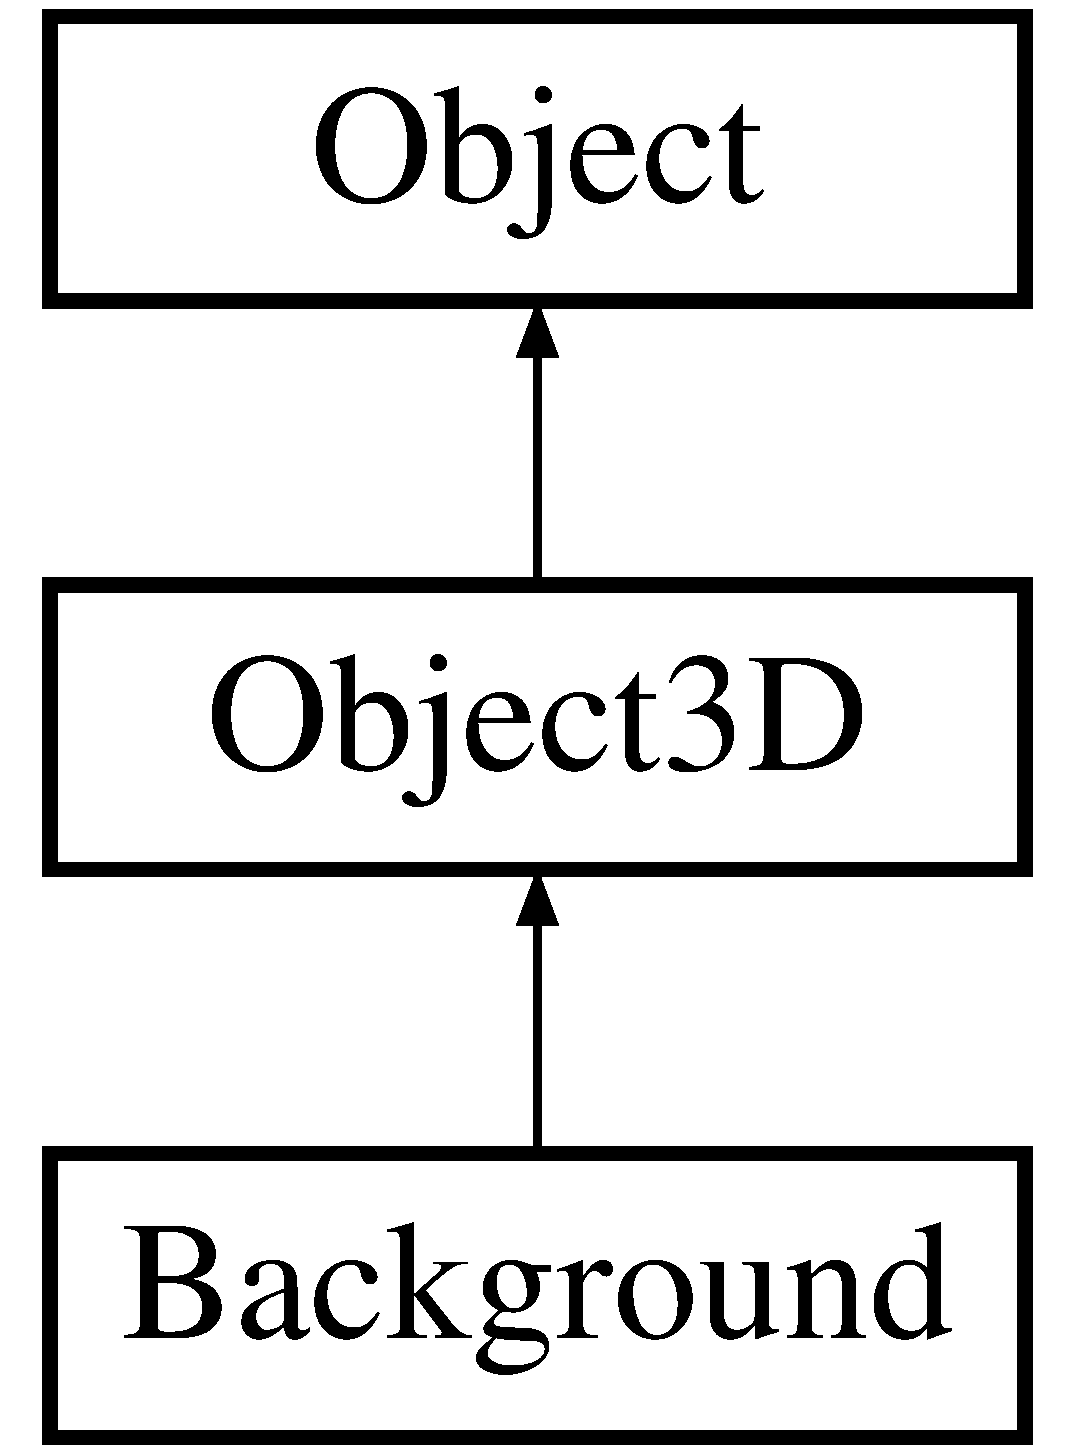
\includegraphics[height=2cm]{classm3g_1_1Background}
\end{center}
\end{figure}
\subsection*{Classes}
\begin{CompactItemize}
\item 
struct \textbf{CropRect}
\item 
struct \textbf{ImageMode}
\end{CompactItemize}
\subsection*{Public Member Functions}
\begin{CompactItemize}
\item 
\hyperlink{classm3g_1_1Background_2bbc220bb63956558a8603a7909c2bbd}{Background} ()
\item 
virtual \hyperlink{classm3g_1_1Background_b793cb50870532320856acdd2caf84c3}{$\sim$Background} ()
\item 
\hypertarget{classm3g_1_1Background_415c0b110f95410ded9b85e5d99a496b}{
virtual void \textbf{addAnimationTrack} (\hyperlink{classm3g_1_1AnimationTrack}{AnimationTrack} $\ast$animation\_\-track)}
\label{classm3g_1_1Background_415c0b110f95410ded9b85e5d99a496b}

\item 
virtual int \hyperlink{classm3g_1_1Background_8aad1ceab4c2a03609c8a42324ce484d}{animate} (int world\_\-time)
\item 
int \hyperlink{classm3g_1_1Background_4cfa1931c265ec3412fe3f6408a1b4f5}{getColor} () const 
\item 
int \hyperlink{classm3g_1_1Background_d6d9d6f23b7bb004c93642bcd081f4a3}{getCropHeight} () const 
\item 
int \hyperlink{classm3g_1_1Background_5c6515f6706675ef31ca5dfa0a03b953}{getCropWidth} () const 
\item 
int \hyperlink{classm3g_1_1Background_d0ba0211183decc8f0459ca598b12912}{getCropX} () const 
\item 
int \hyperlink{classm3g_1_1Background_9ef03b219415a1f08aef6745ad5d87d0}{getCropY} () const 
\item 
\hyperlink{classm3g_1_1Image2D}{Image2D} $\ast$ \hyperlink{classm3g_1_1Background_a8c0193b0e7d47d4b5c9f60df24c44f5}{getImage} () const 
\item 
int \hyperlink{classm3g_1_1Background_0dd60d498f4d50d8808c0b3ad61bc9e8}{getImageModeX} () const 
\item 
int \hyperlink{classm3g_1_1Background_a8d38d66f133ae417956a5dc5f84551d}{getImageModeY} () const 
\item 
bool \hyperlink{classm3g_1_1Background_d6b7bfdf4225b509549e2fbb9575b509}{isColorClearEnabled} () const 
\item 
bool \hyperlink{classm3g_1_1Background_d20a03183cd1c6418dcadf94ac0ca470}{isDepthClearEnabled} () const 
\item 
void \hyperlink{classm3g_1_1Background_38439e862c59a31b90e57c18669061ae}{setColor} (int argb)
\item 
void \hyperlink{classm3g_1_1Background_68e4fe4cf32fe60f166056115081aa65}{setColorClearEnable} (bool enable)
\item 
void \hyperlink{classm3g_1_1Background_e543ac6196bbe65a7af8e6b8686441a7}{setCrop} (int crop\_\-x, int rop\_\-y, int width, int height)
\item 
void \hyperlink{classm3g_1_1Background_0953a713c22fd40cd586bcd8af80075a}{setDepthClearEnable} (bool enable)
\item 
void \hyperlink{classm3g_1_1Background_705b89b41cd1b38f664ed912be44baaa}{setImage} (\hyperlink{classm3g_1_1Image2D}{Image2D} $\ast$image)
\item 
\hypertarget{classm3g_1_1Background_aba37cb460a2376f1a4722eebb4de9a9}{
void \textbf{setImageMode} (int mode\_\-x, int mode\_\-y)}
\label{classm3g_1_1Background_aba37cb460a2376f1a4722eebb4de9a9}

\item 
virtual std::ostream \& \hyperlink{classm3g_1_1Background_6fea17fa1532df3794f8cb39cb4f911f}{print} (std::ostream \&out) const 
\end{CompactItemize}
\subsection*{Static Public Attributes}
\begin{CompactItemize}
\item 
static const int \hyperlink{classm3g_1_1Background_ee380e01b33e589c24984e4c4c1c6501}{BORDER} = 32
\item 
static const int \hyperlink{classm3g_1_1Background_a466d02b3d88f856854d0a0955be32e8}{REPEAT} = 33
\end{CompactItemize}
\subsection*{Friends}
\begin{CompactItemize}
\item 
\hypertarget{classm3g_1_1Background_7b4bcdf992c21ae83363f25df05b1d25}{
class \textbf{World}}
\label{classm3g_1_1Background_7b4bcdf992c21ae83363f25df05b1d25}

\end{CompactItemize}


\subsection{Detailed Description}
Defines whether and how to clear the viewport. 

\subsection{Constructor \& Destructor Documentation}
\hypertarget{classm3g_1_1Background_2bbc220bb63956558a8603a7909c2bbd}{
\index{m3g::Background@{m3g::Background}!Background@{Background}}
\index{Background@{Background}!m3g::Background@{m3g::Background}}
\subsubsection[{Background}]{\setlength{\rightskip}{0pt plus 5cm}{\bf Background} ()}}
\label{classm3g_1_1Background_2bbc220bb63956558a8603a7909c2bbd}


Construct a new Backgrround with default values. \hypertarget{classm3g_1_1Background_b793cb50870532320856acdd2caf84c3}{
\index{m3g::Background@{m3g::Background}!$\sim$Background@{$\sim$Background}}
\index{$\sim$Background@{$\sim$Background}!m3g::Background@{m3g::Background}}
\subsubsection[{$\sim$Background}]{\setlength{\rightskip}{0pt plus 5cm}$\sim${\bf Background} ()\hspace{0.3cm}{\tt  \mbox{[}virtual\mbox{]}}}}
\label{classm3g_1_1Background_b793cb50870532320856acdd2caf84c3}


このBackgroundクラスのデストラクタ. 

\subsection{Member Function Documentation}
\hypertarget{classm3g_1_1Background_8aad1ceab4c2a03609c8a42324ce484d}{
\index{m3g::Background@{m3g::Background}!animate@{animate}}
\index{animate@{animate}!m3g::Background@{m3g::Background}}
\subsubsection[{animate}]{\setlength{\rightskip}{0pt plus 5cm}int animate (int {\em world\_\-time})\hspace{0.3cm}{\tt  \mbox{[}virtual\mbox{]}}}}
\label{classm3g_1_1Background_8aad1ceab4c2a03609c8a42324ce484d}


Updates all animated properties in this \hyperlink{classm3g_1_1Object3D}{Object3D} and all Object3Ds that are reachable from this \hyperlink{classm3g_1_1Object3D}{Object3D}. 

Reimplemented from \hyperlink{classm3g_1_1Object3D_8aad1ceab4c2a03609c8a42324ce484d}{Object3D}.\hypertarget{classm3g_1_1Background_4cfa1931c265ec3412fe3f6408a1b4f5}{
\index{m3g::Background@{m3g::Background}!getColor@{getColor}}
\index{getColor@{getColor}!m3g::Background@{m3g::Background}}
\subsubsection[{getColor}]{\setlength{\rightskip}{0pt plus 5cm}int getColor () const}}
\label{classm3g_1_1Background_4cfa1931c265ec3412fe3f6408a1b4f5}


Retrieves the current background color. \hypertarget{classm3g_1_1Background_d6d9d6f23b7bb004c93642bcd081f4a3}{
\index{m3g::Background@{m3g::Background}!getCropHeight@{getCropHeight}}
\index{getCropHeight@{getCropHeight}!m3g::Background@{m3g::Background}}
\subsubsection[{getCropHeight}]{\setlength{\rightskip}{0pt plus 5cm}int getCropHeight () const}}
\label{classm3g_1_1Background_d6d9d6f23b7bb004c93642bcd081f4a3}


Gets the current cropping rectangle height within the source image. \hypertarget{classm3g_1_1Background_5c6515f6706675ef31ca5dfa0a03b953}{
\index{m3g::Background@{m3g::Background}!getCropWidth@{getCropWidth}}
\index{getCropWidth@{getCropWidth}!m3g::Background@{m3g::Background}}
\subsubsection[{getCropWidth}]{\setlength{\rightskip}{0pt plus 5cm}int getCropWidth () const}}
\label{classm3g_1_1Background_5c6515f6706675ef31ca5dfa0a03b953}


Gets the current cropping rectangle width within the source image. \hypertarget{classm3g_1_1Background_d0ba0211183decc8f0459ca598b12912}{
\index{m3g::Background@{m3g::Background}!getCropX@{getCropX}}
\index{getCropX@{getCropX}!m3g::Background@{m3g::Background}}
\subsubsection[{getCropX}]{\setlength{\rightskip}{0pt plus 5cm}int getCropX () const}}
\label{classm3g_1_1Background_d0ba0211183decc8f0459ca598b12912}


Retrieves the current cropping recttangle X offset relativ to the source image top left corner. \hypertarget{classm3g_1_1Background_9ef03b219415a1f08aef6745ad5d87d0}{
\index{m3g::Background@{m3g::Background}!getCropY@{getCropY}}
\index{getCropY@{getCropY}!m3g::Background@{m3g::Background}}
\subsubsection[{getCropY}]{\setlength{\rightskip}{0pt plus 5cm}int getCropY () const}}
\label{classm3g_1_1Background_9ef03b219415a1f08aef6745ad5d87d0}


Retrieves the current cropping recttangle Y offset relativ to the source image top left corner. \hypertarget{classm3g_1_1Background_a8c0193b0e7d47d4b5c9f60df24c44f5}{
\index{m3g::Background@{m3g::Background}!getImage@{getImage}}
\index{getImage@{getImage}!m3g::Background@{m3g::Background}}
\subsubsection[{getImage}]{\setlength{\rightskip}{0pt plus 5cm}{\bf Image2D} $\ast$ getImage () const}}
\label{classm3g_1_1Background_a8c0193b0e7d47d4b5c9f60df24c44f5}


Gets the current background image. \hypertarget{classm3g_1_1Background_0dd60d498f4d50d8808c0b3ad61bc9e8}{
\index{m3g::Background@{m3g::Background}!getImageModeX@{getImageModeX}}
\index{getImageModeX@{getImageModeX}!m3g::Background@{m3g::Background}}
\subsubsection[{getImageModeX}]{\setlength{\rightskip}{0pt plus 5cm}int getImageModeX () const}}
\label{classm3g_1_1Background_0dd60d498f4d50d8808c0b3ad61bc9e8}


Gets the current background image repeat mode for the X dimensiton. \hypertarget{classm3g_1_1Background_a8d38d66f133ae417956a5dc5f84551d}{
\index{m3g::Background@{m3g::Background}!getImageModeY@{getImageModeY}}
\index{getImageModeY@{getImageModeY}!m3g::Background@{m3g::Background}}
\subsubsection[{getImageModeY}]{\setlength{\rightskip}{0pt plus 5cm}int getImageModeY () const}}
\label{classm3g_1_1Background_a8d38d66f133ae417956a5dc5f84551d}


Gets the current background image repeat mode for the Y dimensiton. \hypertarget{classm3g_1_1Background_d6b7bfdf4225b509549e2fbb9575b509}{
\index{m3g::Background@{m3g::Background}!isColorClearEnabled@{isColorClearEnabled}}
\index{isColorClearEnabled@{isColorClearEnabled}!m3g::Background@{m3g::Background}}
\subsubsection[{isColorClearEnabled}]{\setlength{\rightskip}{0pt plus 5cm}bool isColorClearEnabled () const}}
\label{classm3g_1_1Background_d6b7bfdf4225b509549e2fbb9575b509}


Queries whether color buffer clearing is enabled. \hypertarget{classm3g_1_1Background_d20a03183cd1c6418dcadf94ac0ca470}{
\index{m3g::Background@{m3g::Background}!isDepthClearEnabled@{isDepthClearEnabled}}
\index{isDepthClearEnabled@{isDepthClearEnabled}!m3g::Background@{m3g::Background}}
\subsubsection[{isDepthClearEnabled}]{\setlength{\rightskip}{0pt plus 5cm}bool isDepthClearEnabled () const}}
\label{classm3g_1_1Background_d20a03183cd1c6418dcadf94ac0ca470}


Queries whether depth buffer clearing is enabled. \hypertarget{classm3g_1_1Background_6fea17fa1532df3794f8cb39cb4f911f}{
\index{m3g::Background@{m3g::Background}!print@{print}}
\index{print@{print}!m3g::Background@{m3g::Background}}
\subsubsection[{print}]{\setlength{\rightskip}{0pt plus 5cm}std::ostream \& print (std::ostream \& {\em out}) const\hspace{0.3cm}{\tt  \mbox{[}virtual\mbox{]}}}}
\label{classm3g_1_1Background_6fea17fa1532df3794f8cb39cb4f911f}


Print out information of this object, for debug only. 

Reimplemented from \hyperlink{classm3g_1_1Object3D_6fea17fa1532df3794f8cb39cb4f911f}{Object3D}.\hypertarget{classm3g_1_1Background_38439e862c59a31b90e57c18669061ae}{
\index{m3g::Background@{m3g::Background}!setColor@{setColor}}
\index{setColor@{setColor}!m3g::Background@{m3g::Background}}
\subsubsection[{setColor}]{\setlength{\rightskip}{0pt plus 5cm}void setColor (int {\em argb})}}
\label{classm3g_1_1Background_38439e862c59a31b90e57c18669061ae}


Sets the background color. \hypertarget{classm3g_1_1Background_68e4fe4cf32fe60f166056115081aa65}{
\index{m3g::Background@{m3g::Background}!setColorClearEnable@{setColorClearEnable}}
\index{setColorClearEnable@{setColorClearEnable}!m3g::Background@{m3g::Background}}
\subsubsection[{setColorClearEnable}]{\setlength{\rightskip}{0pt plus 5cm}void setColorClearEnable (bool {\em enable})}}
\label{classm3g_1_1Background_68e4fe4cf32fe60f166056115081aa65}


Enables or disables color buffer clearing. \hypertarget{classm3g_1_1Background_e543ac6196bbe65a7af8e6b8686441a7}{
\index{m3g::Background@{m3g::Background}!setCrop@{setCrop}}
\index{setCrop@{setCrop}!m3g::Background@{m3g::Background}}
\subsubsection[{setCrop}]{\setlength{\rightskip}{0pt plus 5cm}void setCrop (int {\em crop\_\-x}, \/  int {\em rop\_\-y}, \/  int {\em width}, \/  int {\em height})}}
\label{classm3g_1_1Background_e543ac6196bbe65a7af8e6b8686441a7}


Sets a cropping rectangle within the background image. \hypertarget{classm3g_1_1Background_0953a713c22fd40cd586bcd8af80075a}{
\index{m3g::Background@{m3g::Background}!setDepthClearEnable@{setDepthClearEnable}}
\index{setDepthClearEnable@{setDepthClearEnable}!m3g::Background@{m3g::Background}}
\subsubsection[{setDepthClearEnable}]{\setlength{\rightskip}{0pt plus 5cm}void setDepthClearEnable (bool {\em enable})}}
\label{classm3g_1_1Background_0953a713c22fd40cd586bcd8af80075a}


Enables or disables depth buffer clearing. \hypertarget{classm3g_1_1Background_705b89b41cd1b38f664ed912be44baaa}{
\index{m3g::Background@{m3g::Background}!setImage@{setImage}}
\index{setImage@{setImage}!m3g::Background@{m3g::Background}}
\subsubsection[{setImage}]{\setlength{\rightskip}{0pt plus 5cm}void setImage ({\bf Image2D} $\ast$ {\em image})}}
\label{classm3g_1_1Background_705b89b41cd1b38f664ed912be44baaa}


Sets the background image, or switches from background image mode to background color mode. 

\subsection{Member Data Documentation}
\hypertarget{classm3g_1_1Background_ee380e01b33e589c24984e4c4c1c6501}{
\index{m3g::Background@{m3g::Background}!BORDER@{BORDER}}
\index{BORDER@{BORDER}!m3g::Background@{m3g::Background}}
\subsubsection[{BORDER}]{\setlength{\rightskip}{0pt plus 5cm}const int {\bf BORDER} = 32\hspace{0.3cm}{\tt  \mbox{[}static\mbox{]}}}}
\label{classm3g_1_1Background_ee380e01b33e589c24984e4c4c1c6501}


Specifies that the imaginary pixels outside of the source image bondaries in X or Y direction are considered to have the background color. \hypertarget{classm3g_1_1Background_a466d02b3d88f856854d0a0955be32e8}{
\index{m3g::Background@{m3g::Background}!REPEAT@{REPEAT}}
\index{REPEAT@{REPEAT}!m3g::Background@{m3g::Background}}
\subsubsection[{REPEAT}]{\setlength{\rightskip}{0pt plus 5cm}const int {\bf REPEAT} = 33\hspace{0.3cm}{\tt  \mbox{[}static\mbox{]}}}}
\label{classm3g_1_1Background_a466d02b3d88f856854d0a0955be32e8}


Specifies that the imaginary pixels outside of the source image bondaries in X or Y direction are considered to have the same color as the pixel in the correspondign position in the source iamge. 

The documentation for this class was generated from the following files:\begin{CompactItemize}
\item 
/work/desktop-m3g/src/Background.hpp\item 
/work/desktop-m3g/src/Background.cpp\end{CompactItemize}

\hypertarget{classm3g_1_1Bone}{
\section{クラス Bone}
\label{classm3g_1_1Bone}\index{m3g::Bone@{m3g::Bone}}
}
{\tt \#include $<$Bone.hpp$>$}

\subsection*{Public メソッド}
\begin{CompactItemize}
\item 
\hypertarget{classm3g_1_1Bone_62fff0696edaffc0a50a77b4bc4529e9}{
\textbf{Bone} (\hyperlink{classm3g_1_1Node}{Node} $\ast$node, int weight, int first\_\-vertex, int num\_\-vertex)}
\label{classm3g_1_1Bone_62fff0696edaffc0a50a77b4bc4529e9}

\item 
\hypertarget{classm3g_1_1Bone_cc495b3a2c429e933dc04e4498a62935}{
\hyperlink{classm3g_1_1Matrix}{Matrix} \textbf{getInverseBindMatrix} () const }
\label{classm3g_1_1Bone_cc495b3a2c429e933dc04e4498a62935}

\item 
\hypertarget{classm3g_1_1Bone_14956dd171d88884e97c459acfd0fd91}{
void \textbf{setInverseBindMatrix} (\hyperlink{classm3g_1_1Matrix}{Matrix} mat)}
\label{classm3g_1_1Bone_14956dd171d88884e97c459acfd0fd91}

\item 
\hypertarget{classm3g_1_1Bone_f1521ea84960548ee9818ae79289ea8a}{
float \textbf{getWeight} (int vertex\_\-index) const }
\label{classm3g_1_1Bone_f1521ea84960548ee9818ae79289ea8a}

\item 
\hypertarget{classm3g_1_1Bone_6fea17fa1532df3794f8cb39cb4f911f}{
std::ostream \& \textbf{print} (std::ostream \&out) const }
\label{classm3g_1_1Bone_6fea17fa1532df3794f8cb39cb4f911f}

\end{CompactItemize}
\subsection*{Public 変数}
\begin{CompactItemize}
\item 
\hypertarget{classm3g_1_1Bone_b88cd70dad2e152cea983610f2a16e68}{
\hyperlink{classm3g_1_1Node}{Node} $\ast$ \textbf{node}}
\label{classm3g_1_1Bone_b88cd70dad2e152cea983610f2a16e68}

\item 
\hypertarget{classm3g_1_1Bone_a01147b1f07072d246c76dc85d69df7c}{
int \textbf{weight}}
\label{classm3g_1_1Bone_a01147b1f07072d246c76dc85d69df7c}

\item 
\hypertarget{classm3g_1_1Bone_f6fef1fff206a6d6fcfcc1287b45ace6}{
int \textbf{first\_\-vertex}}
\label{classm3g_1_1Bone_f6fef1fff206a6d6fcfcc1287b45ace6}

\item 
\hypertarget{classm3g_1_1Bone_f130b7ed1451b2713ca985fd292e2e4a}{
int \textbf{num\_\-vertex}}
\label{classm3g_1_1Bone_f130b7ed1451b2713ca985fd292e2e4a}

\item 
\hypertarget{classm3g_1_1Bone_564e81227889d6b0b01e707d49f26f10}{
\hyperlink{classm3g_1_1Matrix}{Matrix} \textbf{inv\_\-bind\_\-matrix}}
\label{classm3g_1_1Bone_564e81227889d6b0b01e707d49f26f10}

\end{CompactItemize}


\subsection{説明}
ボーンを表すM3Gの定義外の内部使用のクラス. 

このクラスの説明は次のファイルから生成されました:\begin{CompactItemize}
\item 
/work/desktop-m3g/src/Bone.hpp\item 
/work/desktop-m3g/src/Bone.cpp\end{CompactItemize}

\hypertarget{classm3g_1_1Camera}{
\section{Camera Class Reference}
\label{classm3g_1_1Camera}\index{m3g::Camera@{m3g::Camera}}
}
{\tt \#include $<$Camera.hpp$>$}

Inheritance diagram for Camera::\begin{figure}[H]
\begin{center}
\leavevmode
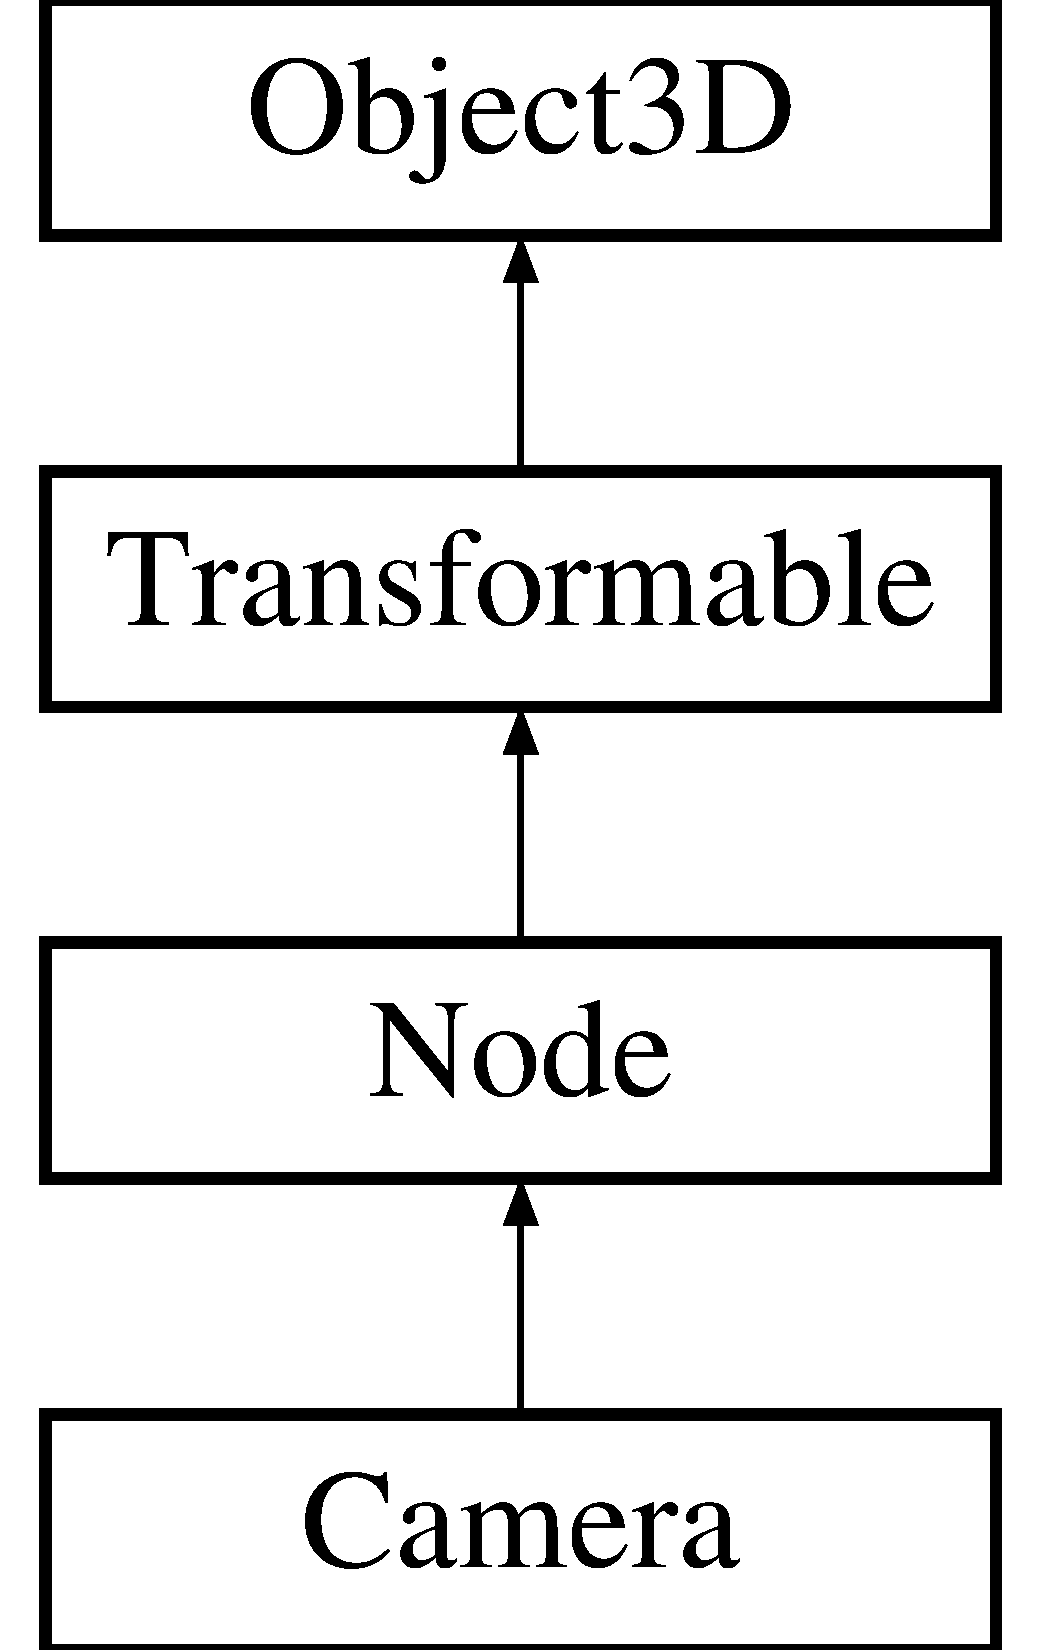
\includegraphics[height=4cm]{classm3g_1_1Camera}
\end{center}
\end{figure}
\subsection*{Public Member Functions}
\begin{CompactItemize}
\item 
\hyperlink{classm3g_1_1Camera_a3f3efcb2fcc75de885df29041103cd2}{Camera} ()
\item 
virtual \hyperlink{classm3g_1_1Camera_b921e886e6f14e117eb8099ccb0a3775}{$\sim$Camera} ()
\item 
virtual void \hyperlink{classm3g_1_1Camera_415c0b110f95410ded9b85e5d99a496b}{addAnimationTrack} (\hyperlink{classm3g_1_1AnimationTrack}{AnimationTrack} $\ast$animation\_\-track)
\item 
virtual int \hyperlink{classm3g_1_1Camera_8aad1ceab4c2a03609c8a42324ce484d}{animate} (int world\_\-time)
\item 
int \hyperlink{classm3g_1_1Camera_a2ebe46a4e16fee86d4f547588411302}{getProjection} (float $\ast$params) const 
\item 
int \hyperlink{classm3g_1_1Camera_9e0c204df146342990703acb744954b1}{getProjection} (\hyperlink{classm3g_1_1Transform}{Transform} $\ast$transform) const 
\item 
void \hyperlink{classm3g_1_1Camera_51c42821097e90d3f59e87676684f60a}{setGeneric} (const \hyperlink{classm3g_1_1Transform}{Transform} \&transorm)
\item 
void \hyperlink{classm3g_1_1Camera_88ecc1c18e2d785ca9638e0bec6c5ce2}{setParallel} (float fovy, float aspect\_\-ratio, float near, float far)
\item 
void \hyperlink{classm3g_1_1Camera_ca92a48ebe3424deac8e54c27550189d}{setPerspective} (float fovy, float aspect\_\-ratio, float near, float far)
\item 
virtual std::ostream \& \hyperlink{classm3g_1_1Camera_6fea17fa1532df3794f8cb39cb4f911f}{print} (std::ostream \&out) const 
\item 
void \hyperlink{classm3g_1_1Camera_0006b18ae0e27a031d533e987b9756a8}{lookAt} (float from\_\-x, float from\_\-y, float from\_\-z, float to\_\-x, float to\_\-y, float to\_\-z, float up\_\-x, float up\_\-y, float up\_\-z)
\end{CompactItemize}
\subsection*{Static Public Attributes}
\begin{CompactItemize}
\item 
static const int \hyperlink{classm3g_1_1Camera_48a4e153c97a1f4890558a77dfe02ca4}{GENERIC} = 48
\item 
static const int \hyperlink{classm3g_1_1Camera_d9630da0e9505afbb107c86229aa2f08}{PARALLEL} = 49
\item 
static const int \hyperlink{classm3g_1_1Camera_e62e72bde93e7d7ceb482e7a8c40dcf5}{PERSPECTIVE} = 50
\end{CompactItemize}
\subsection*{Protected Member Functions}
\begin{CompactItemize}
\item 
virtual void \hyperlink{classm3g_1_1Camera_1efcb1973989d9963d5bd6d03065d389}{render} (int pass, int index=0) const 
\end{CompactItemize}
\subsection*{Friends}
\begin{CompactItemize}
\item 
\hypertarget{classm3g_1_1Camera_8174d4c629550c1ee279571250236ef4}{
class \textbf{Graphics3D}}
\label{classm3g_1_1Camera_8174d4c629550c1ee279571250236ef4}

\item 
\hypertarget{classm3g_1_1Camera_7b4bcdf992c21ae83363f25df05b1d25}{
class \textbf{World}}
\label{classm3g_1_1Camera_7b4bcdf992c21ae83363f25df05b1d25}

\end{CompactItemize}


\subsection{Detailed Description}
A scene graph node that defines the position of the viewer in the scene and the projection from 3D to 2D. 

\subsection{Constructor \& Destructor Documentation}
\hypertarget{classm3g_1_1Camera_a3f3efcb2fcc75de885df29041103cd2}{
\index{m3g::Camera@{m3g::Camera}!Camera@{Camera}}
\index{Camera@{Camera}!m3g::Camera@{m3g::Camera}}
\subsubsection[{Camera}]{\setlength{\rightskip}{0pt plus 5cm}{\bf Camera} ()}}
\label{classm3g_1_1Camera_a3f3efcb2fcc75de885df29041103cd2}


Constructs a new \hyperlink{classm3g_1_1Camera}{Camera} node with default values. \hypertarget{classm3g_1_1Camera_b921e886e6f14e117eb8099ccb0a3775}{
\index{m3g::Camera@{m3g::Camera}!$\sim$Camera@{$\sim$Camera}}
\index{$\sim$Camera@{$\sim$Camera}!m3g::Camera@{m3g::Camera}}
\subsubsection[{$\sim$Camera}]{\setlength{\rightskip}{0pt plus 5cm}$\sim${\bf Camera} ()\hspace{0.3cm}{\tt  \mbox{[}virtual\mbox{]}}}}
\label{classm3g_1_1Camera_b921e886e6f14e117eb8099ccb0a3775}


Destruct a \hyperlink{classm3g_1_1Camera}{Camera} node. 

\subsection{Member Function Documentation}
\hypertarget{classm3g_1_1Camera_415c0b110f95410ded9b85e5d99a496b}{
\index{m3g::Camera@{m3g::Camera}!addAnimationTrack@{addAnimationTrack}}
\index{addAnimationTrack@{addAnimationTrack}!m3g::Camera@{m3g::Camera}}
\subsubsection[{addAnimationTrack}]{\setlength{\rightskip}{0pt plus 5cm}void addAnimationTrack ({\bf AnimationTrack} $\ast$ {\em animation\_\-track})\hspace{0.3cm}{\tt  \mbox{[}virtual\mbox{]}}}}
\label{classm3g_1_1Camera_415c0b110f95410ded9b85e5d99a496b}


Adds the given \hyperlink{classm3g_1_1AnimationTrack}{AnimationTrack} to this \hyperlink{classm3g_1_1Object3D}{Object3D}, potentially chaing the order and indices of the previously added tracks. 

Reimplemented from \hyperlink{classm3g_1_1Node_415c0b110f95410ded9b85e5d99a496b}{Node}.\hypertarget{classm3g_1_1Camera_8aad1ceab4c2a03609c8a42324ce484d}{
\index{m3g::Camera@{m3g::Camera}!animate@{animate}}
\index{animate@{animate}!m3g::Camera@{m3g::Camera}}
\subsubsection[{animate}]{\setlength{\rightskip}{0pt plus 5cm}int animate (int {\em world\_\-time})\hspace{0.3cm}{\tt  \mbox{[}virtual\mbox{]}}}}
\label{classm3g_1_1Camera_8aad1ceab4c2a03609c8a42324ce484d}


Update animatable property to specified world time. 

Reimplemented from \hyperlink{classm3g_1_1Node_8aad1ceab4c2a03609c8a42324ce484d}{Node}.\hypertarget{classm3g_1_1Camera_9e0c204df146342990703acb744954b1}{
\index{m3g::Camera@{m3g::Camera}!getProjection@{getProjection}}
\index{getProjection@{getProjection}!m3g::Camera@{m3g::Camera}}
\subsubsection[{getProjection}]{\setlength{\rightskip}{0pt plus 5cm}int getProjection ({\bf Transform} $\ast$ {\em transform}) const}}
\label{classm3g_1_1Camera_9e0c204df146342990703acb744954b1}


Gets the current projection matrix and type. \hypertarget{classm3g_1_1Camera_a2ebe46a4e16fee86d4f547588411302}{
\index{m3g::Camera@{m3g::Camera}!getProjection@{getProjection}}
\index{getProjection@{getProjection}!m3g::Camera@{m3g::Camera}}
\subsubsection[{getProjection}]{\setlength{\rightskip}{0pt plus 5cm}int getProjection (float $\ast$ {\em params}) const}}
\label{classm3g_1_1Camera_a2ebe46a4e16fee86d4f547588411302}


Gets the current projection matrix and type. \hypertarget{classm3g_1_1Camera_0006b18ae0e27a031d533e987b9756a8}{
\index{m3g::Camera@{m3g::Camera}!lookAt@{lookAt}}
\index{lookAt@{lookAt}!m3g::Camera@{m3g::Camera}}
\subsubsection[{lookAt}]{\setlength{\rightskip}{0pt plus 5cm}void lookAt (float {\em from\_\-x}, \/  float {\em from\_\-y}, \/  float {\em from\_\-z}, \/  float {\em to\_\-x}, \/  float {\em to\_\-y}, \/  float {\em to\_\-z}, \/  float {\em up\_\-x}, \/  float {\em up\_\-y}, \/  float {\em up\_\-z})}}
\label{classm3g_1_1Camera_0006b18ae0e27a031d533e987b9756a8}


Same as glut's lookat() function. this is not in M3G. \hypertarget{classm3g_1_1Camera_6fea17fa1532df3794f8cb39cb4f911f}{
\index{m3g::Camera@{m3g::Camera}!print@{print}}
\index{print@{print}!m3g::Camera@{m3g::Camera}}
\subsubsection[{print}]{\setlength{\rightskip}{0pt plus 5cm}std::ostream \& print (std::ostream \& {\em out}) const\hspace{0.3cm}{\tt  \mbox{[}virtual\mbox{]}}}}
\label{classm3g_1_1Camera_6fea17fa1532df3794f8cb39cb4f911f}


print out information of this calss, for debug only. 

Reimplemented from \hyperlink{classm3g_1_1Node_6fea17fa1532df3794f8cb39cb4f911f}{Node}.\hypertarget{classm3g_1_1Camera_1efcb1973989d9963d5bd6d03065d389}{
\index{m3g::Camera@{m3g::Camera}!render@{render}}
\index{render@{render}!m3g::Camera@{m3g::Camera}}
\subsubsection[{render}]{\setlength{\rightskip}{0pt plus 5cm}void render (int {\em pass}, \/  int {\em index} = {\tt 0}) const\hspace{0.3cm}{\tt  \mbox{[}protected, virtual\mbox{]}}}}
\label{classm3g_1_1Camera_1efcb1973989d9963d5bd6d03065d389}


Render this Camear object, for inner use.

Note: \hyperlink{classm3g_1_1Camera}{Camera} should be rendered only at 0th rendering pass(pass=0). In other cases, do nothing. 

Reimplemented from \hyperlink{classm3g_1_1Node_1efcb1973989d9963d5bd6d03065d389}{Node}.\hypertarget{classm3g_1_1Camera_51c42821097e90d3f59e87676684f60a}{
\index{m3g::Camera@{m3g::Camera}!setGeneric@{setGeneric}}
\index{setGeneric@{setGeneric}!m3g::Camera@{m3g::Camera}}
\subsubsection[{setGeneric}]{\setlength{\rightskip}{0pt plus 5cm}void setGeneric (const {\bf Transform} \& {\em transorm})}}
\label{classm3g_1_1Camera_51c42821097e90d3f59e87676684f60a}


Sets the given x4 transformation as the current projcetion matrix. \hypertarget{classm3g_1_1Camera_88ecc1c18e2d785ca9638e0bec6c5ce2}{
\index{m3g::Camera@{m3g::Camera}!setParallel@{setParallel}}
\index{setParallel@{setParallel}!m3g::Camera@{m3g::Camera}}
\subsubsection[{setParallel}]{\setlength{\rightskip}{0pt plus 5cm}void setParallel (float {\em fovy}, \/  float {\em aspect\_\-ratio}, \/  float {\em near}, \/  float {\em far})}}
\label{classm3g_1_1Camera_88ecc1c18e2d785ca9638e0bec6c5ce2}


Constructs a parallel projection matrix and sets that as the current projcection matrix. \hypertarget{classm3g_1_1Camera_ca92a48ebe3424deac8e54c27550189d}{
\index{m3g::Camera@{m3g::Camera}!setPerspective@{setPerspective}}
\index{setPerspective@{setPerspective}!m3g::Camera@{m3g::Camera}}
\subsubsection[{setPerspective}]{\setlength{\rightskip}{0pt plus 5cm}void setPerspective (float {\em fovy}, \/  float {\em aspect\_\-ratio}, \/  float {\em near}, \/  float {\em far})}}
\label{classm3g_1_1Camera_ca92a48ebe3424deac8e54c27550189d}


Constructs a perspective projection matrix and sets that as the current projection matrix. 

\subsection{Member Data Documentation}
\hypertarget{classm3g_1_1Camera_48a4e153c97a1f4890558a77dfe02ca4}{
\index{m3g::Camera@{m3g::Camera}!GENERIC@{GENERIC}}
\index{GENERIC@{GENERIC}!m3g::Camera@{m3g::Camera}}
\subsubsection[{GENERIC}]{\setlength{\rightskip}{0pt plus 5cm}const int {\bf GENERIC} = 48\hspace{0.3cm}{\tt  \mbox{[}static\mbox{]}}}}
\label{classm3g_1_1Camera_48a4e153c97a1f4890558a77dfe02ca4}


Specifies a generic 4x4 projection matrix. \hypertarget{classm3g_1_1Camera_d9630da0e9505afbb107c86229aa2f08}{
\index{m3g::Camera@{m3g::Camera}!PARALLEL@{PARALLEL}}
\index{PARALLEL@{PARALLEL}!m3g::Camera@{m3g::Camera}}
\subsubsection[{PARALLEL}]{\setlength{\rightskip}{0pt plus 5cm}const int {\bf PARALLEL} = 49\hspace{0.3cm}{\tt  \mbox{[}static\mbox{]}}}}
\label{classm3g_1_1Camera_d9630da0e9505afbb107c86229aa2f08}


Specifies a parallel projection matrix. \hypertarget{classm3g_1_1Camera_e62e72bde93e7d7ceb482e7a8c40dcf5}{
\index{m3g::Camera@{m3g::Camera}!PERSPECTIVE@{PERSPECTIVE}}
\index{PERSPECTIVE@{PERSPECTIVE}!m3g::Camera@{m3g::Camera}}
\subsubsection[{PERSPECTIVE}]{\setlength{\rightskip}{0pt plus 5cm}const int {\bf PERSPECTIVE} = 50\hspace{0.3cm}{\tt  \mbox{[}static\mbox{]}}}}
\label{classm3g_1_1Camera_e62e72bde93e7d7ceb482e7a8c40dcf5}


specifies a perspective projection matrix. 

The documentation for this class was generated from the following files:\begin{CompactItemize}
\item 
/work/desktop-m3g/src/Camera.hpp\item 
/work/desktop-m3g/src/Camera.cpp\end{CompactItemize}

\hypertarget{classm3g_1_1CompositingMode}{
\section{クラス CompositingMode}
\label{classm3g_1_1CompositingMode}\index{m3g::CompositingMode@{m3g::CompositingMode}}
}
{\tt \#include $<$CompositingMode.hpp$>$}

CompositingModeに対する継承グラフ:\begin{figure}[H]
\begin{center}
\leavevmode
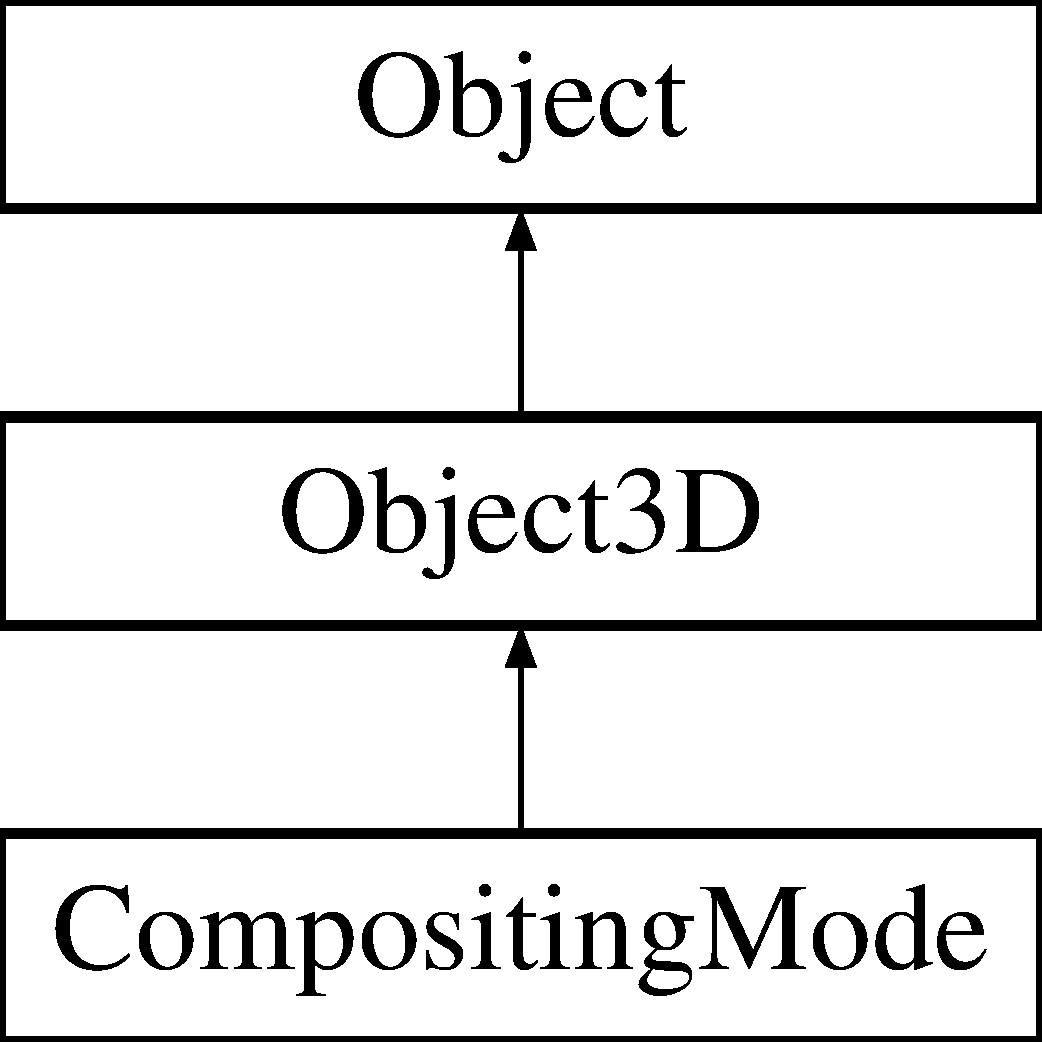
\includegraphics[height=3cm]{classm3g_1_1CompositingMode}
\end{center}
\end{figure}
\subsection*{構成}
\begin{CompactItemize}
\item 
struct \hyperlink{structm3g_1_1CompositingMode_1_1DepthOffset}{DepthOffset}
\end{CompactItemize}
\subsection*{Public メソッド}
\begin{CompactItemize}
\item 
\hyperlink{classm3g_1_1CompositingMode_5abfd1a798f1327aac4b92f55d4ecc0c}{CompositingMode} ()
\item 
virtual \hyperlink{classm3g_1_1CompositingMode_0bba5b15be7249e946c9aaf94631ce3b}{$\sim$CompositingMode} ()
\item 
virtual \hyperlink{classm3g_1_1CompositingMode}{CompositingMode} $\ast$ \hyperlink{classm3g_1_1CompositingMode_ab6fcd945b68728bbe2c65a8f45dc8dd}{duplicate} () const 
\item 
float \hyperlink{classm3g_1_1CompositingMode_19ab71363ea77fa86aa6fafce87f06cb}{getAlphaThreshold} () const 
\item 
int \hyperlink{classm3g_1_1CompositingMode_078954de3d786bd11dc98b06f237bbbb}{getBlending} () const 
\item 
float \hyperlink{classm3g_1_1CompositingMode_d24a4116e72678164f31d7a48f74be6b}{getDepthOffsetFactor} () const 
\item 
float \hyperlink{classm3g_1_1CompositingMode_add4c6c3bc01c1d0689e0588af79039f}{getDepthOffsetUnits} () const 
\item 
bool \hyperlink{classm3g_1_1CompositingMode_bfcec134f769763d492011fc8ccadcce}{isAlphaWriteEnabled} () const 
\item 
bool \hyperlink{classm3g_1_1CompositingMode_35ffa21944393c774552003dd2cb03ea}{isColorWriteEnabled} () const 
\item 
bool \hyperlink{classm3g_1_1CompositingMode_4dd97b29a6e12c5e64477ab1546f93f1}{isDepthTestEnabled} () const 
\item 
bool \hyperlink{classm3g_1_1CompositingMode_0ee4c812abd4a99e0373158d36dc45d9}{isDepthWriteEnabled} () const 
\item 
void \hyperlink{classm3g_1_1CompositingMode_6becafaefd18a2b8b1adeba491576837}{setAlphaThreshold} (float threshold)
\item 
void \hyperlink{classm3g_1_1CompositingMode_5204f1acac056f82d322262703be67b0}{setAlphaWriteEnable} (bool enable)
\item 
void \hyperlink{classm3g_1_1CompositingMode_4c09465dfec9efa000c115c5c2867b63}{setBlending} (int mode)
\item 
void \hyperlink{classm3g_1_1CompositingMode_84f7cba08f5a2bea05de4fc3154a50b2}{setColorWriteEnable} (bool enable)
\item 
void \hyperlink{classm3g_1_1CompositingMode_4c825055ad0b5910ef4f9136d9a8e588}{setDepthOffset} (float factor, float units)
\item 
void \hyperlink{classm3g_1_1CompositingMode_5f1afccdc51665bb04c971579d8ee05c}{setDepthTestEnable} (bool enable)
\item 
void \hyperlink{classm3g_1_1CompositingMode_a3275c9589ef319c6ba6f5c22d0b2860}{setDepthWriteEnable} (bool enable)
\item 
virtual std::ostream \& \hyperlink{classm3g_1_1CompositingMode_6fea17fa1532df3794f8cb39cb4f911f}{print} (std::ostream \&out) const 
\item 
virtual void \hyperlink{classm3g_1_1CompositingMode_8babc8a79b78615da51161e94029eea9}{render} (\hyperlink{structm3g_1_1RenderState}{RenderState} \&state) const 
\end{CompactItemize}
\subsection*{Static Public 変数}
\begin{CompactItemize}
\item 
static const int \hyperlink{classm3g_1_1CompositingMode_417581fcde4067111f47320edb2aa378}{ALPHA} = 64
\item 
static const int \hyperlink{classm3g_1_1CompositingMode_91ac80a5450e5f7f7e382860829030d9}{ALPHA\_\-ADD} = 65
\item 
static const int \hyperlink{classm3g_1_1CompositingMode_96b64c2847348fb73a90c4a501cda9d1}{MODULATE} = 66
\item 
static const int \hyperlink{classm3g_1_1CompositingMode_cb426684e42a5ae425989c65fbb7dbc4}{MODULATE\_\-X2} = 67
\item 
static const int \hyperlink{classm3g_1_1CompositingMode_47a00ac5a59817a48db06fb2a538883c}{REPLACE} = 68
\end{CompactItemize}
\subsection*{フレンド}
\begin{CompactItemize}
\item 
\hypertarget{classm3g_1_1CompositingMode_afa5201a494f65c37039281d9b63a2a9}{
class \textbf{Appearance}}
\label{classm3g_1_1CompositingMode_afa5201a494f65c37039281d9b63a2a9}

\end{CompactItemize}


\subsection{説明}
ピクセル単位のコンポジット方法をカプセル化したアピアランスの構成要素. 

\subsection{コンストラクタとデストラクタ}
\hypertarget{classm3g_1_1CompositingMode_5abfd1a798f1327aac4b92f55d4ecc0c}{
\index{m3g::CompositingMode@{m3g::CompositingMode}!CompositingMode@{CompositingMode}}
\index{CompositingMode@{CompositingMode}!m3g::CompositingMode@{m3g::CompositingMode}}
\subsubsection[{CompositingMode}]{\setlength{\rightskip}{0pt plus 5cm}{\bf CompositingMode} ()}}
\label{classm3g_1_1CompositingMode_5abfd1a798f1327aac4b92f55d4ecc0c}


CompositingModeオブジェクトを作成するコンストラクタ. \hypertarget{classm3g_1_1CompositingMode_0bba5b15be7249e946c9aaf94631ce3b}{
\index{m3g::CompositingMode@{m3g::CompositingMode}!$\sim$CompositingMode@{$\sim$CompositingMode}}
\index{$\sim$CompositingMode@{$\sim$CompositingMode}!m3g::CompositingMode@{m3g::CompositingMode}}
\subsubsection[{$\sim$CompositingMode}]{\setlength{\rightskip}{0pt plus 5cm}$\sim${\bf CompositingMode} ()\hspace{0.3cm}{\tt  \mbox{[}virtual\mbox{]}}}}
\label{classm3g_1_1CompositingMode_0bba5b15be7249e946c9aaf94631ce3b}


このCompositingModeオブジェクトのデストラクタ. 

\subsection{関数}
\hypertarget{classm3g_1_1CompositingMode_ab6fcd945b68728bbe2c65a8f45dc8dd}{
\index{m3g::CompositingMode@{m3g::CompositingMode}!duplicate@{duplicate}}
\index{duplicate@{duplicate}!m3g::CompositingMode@{m3g::CompositingMode}}
\subsubsection[{duplicate}]{\setlength{\rightskip}{0pt plus 5cm}{\bf CompositingMode} $\ast$ duplicate () const\hspace{0.3cm}{\tt  \mbox{[}virtual\mbox{]}}}}
\label{classm3g_1_1CompositingMode_ab6fcd945b68728bbe2c65a8f45dc8dd}


このオブジェクトの複製の作成. 

\hyperlink{classm3g_1_1Object3D_a25110dac934f867b83b73ad4741a0f4}{Object3D}を再定義しています。\hypertarget{classm3g_1_1CompositingMode_19ab71363ea77fa86aa6fafce87f06cb}{
\index{m3g::CompositingMode@{m3g::CompositingMode}!getAlphaThreshold@{getAlphaThreshold}}
\index{getAlphaThreshold@{getAlphaThreshold}!m3g::CompositingMode@{m3g::CompositingMode}}
\subsubsection[{getAlphaThreshold}]{\setlength{\rightskip}{0pt plus 5cm}float getAlphaThreshold () const}}
\label{classm3g_1_1CompositingMode_19ab71363ea77fa86aa6fafce87f06cb}


カレントのαテストの閾値を取得する. \hypertarget{classm3g_1_1CompositingMode_078954de3d786bd11dc98b06f237bbbb}{
\index{m3g::CompositingMode@{m3g::CompositingMode}!getBlending@{getBlending}}
\index{getBlending@{getBlending}!m3g::CompositingMode@{m3g::CompositingMode}}
\subsubsection[{getBlending}]{\setlength{\rightskip}{0pt plus 5cm}int getBlending () const}}
\label{classm3g_1_1CompositingMode_078954de3d786bd11dc98b06f237bbbb}


カレントのフレームバッファーのブレンディングモードを取得する. \hypertarget{classm3g_1_1CompositingMode_d24a4116e72678164f31d7a48f74be6b}{
\index{m3g::CompositingMode@{m3g::CompositingMode}!getDepthOffsetFactor@{getDepthOffsetFactor}}
\index{getDepthOffsetFactor@{getDepthOffsetFactor}!m3g::CompositingMode@{m3g::CompositingMode}}
\subsubsection[{getDepthOffsetFactor}]{\setlength{\rightskip}{0pt plus 5cm}float getDepthOffsetFactor () const}}
\label{classm3g_1_1CompositingMode_d24a4116e72678164f31d7a48f74be6b}


カレントの深度オフセットの勾配値を取得する. \hypertarget{classm3g_1_1CompositingMode_add4c6c3bc01c1d0689e0588af79039f}{
\index{m3g::CompositingMode@{m3g::CompositingMode}!getDepthOffsetUnits@{getDepthOffsetUnits}}
\index{getDepthOffsetUnits@{getDepthOffsetUnits}!m3g::CompositingMode@{m3g::CompositingMode}}
\subsubsection[{getDepthOffsetUnits}]{\setlength{\rightskip}{0pt plus 5cm}float getDepthOffsetUnits () const}}
\label{classm3g_1_1CompositingMode_add4c6c3bc01c1d0689e0588af79039f}


カレントの固定深度オフセット値を取得する. \hypertarget{classm3g_1_1CompositingMode_bfcec134f769763d492011fc8ccadcce}{
\index{m3g::CompositingMode@{m3g::CompositingMode}!isAlphaWriteEnabled@{isAlphaWriteEnabled}}
\index{isAlphaWriteEnabled@{isAlphaWriteEnabled}!m3g::CompositingMode@{m3g::CompositingMode}}
\subsubsection[{isAlphaWriteEnabled}]{\setlength{\rightskip}{0pt plus 5cm}bool isAlphaWriteEnabled () const}}
\label{classm3g_1_1CompositingMode_bfcec134f769763d492011fc8ccadcce}


αチャンネルへの書き込みが有効かどうかの問い合わせ. \hypertarget{classm3g_1_1CompositingMode_35ffa21944393c774552003dd2cb03ea}{
\index{m3g::CompositingMode@{m3g::CompositingMode}!isColorWriteEnabled@{isColorWriteEnabled}}
\index{isColorWriteEnabled@{isColorWriteEnabled}!m3g::CompositingMode@{m3g::CompositingMode}}
\subsubsection[{isColorWriteEnabled}]{\setlength{\rightskip}{0pt plus 5cm}bool isColorWriteEnabled () const}}
\label{classm3g_1_1CompositingMode_35ffa21944393c774552003dd2cb03ea}


カラーチャンネルへの書き込みが有効かどうかの問い合わせ. \hypertarget{classm3g_1_1CompositingMode_4dd97b29a6e12c5e64477ab1546f93f1}{
\index{m3g::CompositingMode@{m3g::CompositingMode}!isDepthTestEnabled@{isDepthTestEnabled}}
\index{isDepthTestEnabled@{isDepthTestEnabled}!m3g::CompositingMode@{m3g::CompositingMode}}
\subsubsection[{isDepthTestEnabled}]{\setlength{\rightskip}{0pt plus 5cm}bool isDepthTestEnabled () const}}
\label{classm3g_1_1CompositingMode_4dd97b29a6e12c5e64477ab1546f93f1}


深度テストが有効かどうかの問い合わせ. \hypertarget{classm3g_1_1CompositingMode_0ee4c812abd4a99e0373158d36dc45d9}{
\index{m3g::CompositingMode@{m3g::CompositingMode}!isDepthWriteEnabled@{isDepthWriteEnabled}}
\index{isDepthWriteEnabled@{isDepthWriteEnabled}!m3g::CompositingMode@{m3g::CompositingMode}}
\subsubsection[{isDepthWriteEnabled}]{\setlength{\rightskip}{0pt plus 5cm}bool isDepthWriteEnabled () const}}
\label{classm3g_1_1CompositingMode_0ee4c812abd4a99e0373158d36dc45d9}


深度バッファーへの書き込みが有効かどうかの問い合わせ. \hypertarget{classm3g_1_1CompositingMode_6fea17fa1532df3794f8cb39cb4f911f}{
\index{m3g::CompositingMode@{m3g::CompositingMode}!print@{print}}
\index{print@{print}!m3g::CompositingMode@{m3g::CompositingMode}}
\subsubsection[{print}]{\setlength{\rightskip}{0pt plus 5cm}std::ostream \& print (std::ostream \& {\em out}) const\hspace{0.3cm}{\tt  \mbox{[}virtual\mbox{]}}}}
\label{classm3g_1_1CompositingMode_6fea17fa1532df3794f8cb39cb4f911f}


このCompositingModeの情報を表示する。デバッグ用. 

\hyperlink{classm3g_1_1Object3D_6fea17fa1532df3794f8cb39cb4f911f}{Object3D}を再定義しています。\hypertarget{classm3g_1_1CompositingMode_8babc8a79b78615da51161e94029eea9}{
\index{m3g::CompositingMode@{m3g::CompositingMode}!render@{render}}
\index{render@{render}!m3g::CompositingMode@{m3g::CompositingMode}}
\subsubsection[{render}]{\setlength{\rightskip}{0pt plus 5cm}void render ({\bf RenderState} \& {\em state}) const\hspace{0.3cm}{\tt  \mbox{[}virtual\mbox{]}}}}
\label{classm3g_1_1CompositingMode_8babc8a79b78615da51161e94029eea9}


このオブジェクトをレンダリングする内部使用の関数.

Note: \hyperlink{classm3g_1_1CompositingMode}{CompositingMode} should be rendered only at second rendering pass(pass=2). In other cases, do nothing. 

\hyperlink{classm3g_1_1Object3D_8babc8a79b78615da51161e94029eea9}{Object3D}を再定義しています。\hypertarget{classm3g_1_1CompositingMode_6becafaefd18a2b8b1adeba491576837}{
\index{m3g::CompositingMode@{m3g::CompositingMode}!setAlphaThreshold@{setAlphaThreshold}}
\index{setAlphaThreshold@{setAlphaThreshold}!m3g::CompositingMode@{m3g::CompositingMode}}
\subsubsection[{setAlphaThreshold}]{\setlength{\rightskip}{0pt plus 5cm}void setAlphaThreshold (float {\em threshold})}}
\label{classm3g_1_1CompositingMode_6becafaefd18a2b8b1adeba491576837}


αテスト閾値の設定. \hypertarget{classm3g_1_1CompositingMode_5204f1acac056f82d322262703be67b0}{
\index{m3g::CompositingMode@{m3g::CompositingMode}!setAlphaWriteEnable@{setAlphaWriteEnable}}
\index{setAlphaWriteEnable@{setAlphaWriteEnable}!m3g::CompositingMode@{m3g::CompositingMode}}
\subsubsection[{setAlphaWriteEnable}]{\setlength{\rightskip}{0pt plus 5cm}void setAlphaWriteEnable (bool {\em enable})}}
\label{classm3g_1_1CompositingMode_5204f1acac056f82d322262703be67b0}


フラグメントのα成分をカラーバッファーへ書き込む事を許可もしくは不許可にする. \hypertarget{classm3g_1_1CompositingMode_4c09465dfec9efa000c115c5c2867b63}{
\index{m3g::CompositingMode@{m3g::CompositingMode}!setBlending@{setBlending}}
\index{setBlending@{setBlending}!m3g::CompositingMode@{m3g::CompositingMode}}
\subsubsection[{setBlending}]{\setlength{\rightskip}{0pt plus 5cm}void setBlending (int {\em mode})}}
\label{classm3g_1_1CompositingMode_4c09465dfec9efa000c115c5c2867b63}


フレームバッファーのピクセルとのブレンドモードの設定. \hypertarget{classm3g_1_1CompositingMode_84f7cba08f5a2bea05de4fc3154a50b2}{
\index{m3g::CompositingMode@{m3g::CompositingMode}!setColorWriteEnable@{setColorWriteEnable}}
\index{setColorWriteEnable@{setColorWriteEnable}!m3g::CompositingMode@{m3g::CompositingMode}}
\subsubsection[{setColorWriteEnable}]{\setlength{\rightskip}{0pt plus 5cm}void setColorWriteEnable (bool {\em enable})}}
\label{classm3g_1_1CompositingMode_84f7cba08f5a2bea05de4fc3154a50b2}


カラーバッファーへのフラグメントのカラーの書き込みの許可もしくは不許可の設定. \hypertarget{classm3g_1_1CompositingMode_4c825055ad0b5910ef4f9136d9a8e588}{
\index{m3g::CompositingMode@{m3g::CompositingMode}!setDepthOffset@{setDepthOffset}}
\index{setDepthOffset@{setDepthOffset}!m3g::CompositingMode@{m3g::CompositingMode}}
\subsubsection[{setDepthOffset}]{\setlength{\rightskip}{0pt plus 5cm}void setDepthOffset (float {\em factor}, \/  float {\em units})}}
\label{classm3g_1_1CompositingMode_4c825055ad0b5910ef4f9136d9a8e588}


深度テストと深度バッファーへの書き込みの直前にスクリーン座標のZ座標にある値を足す. \hypertarget{classm3g_1_1CompositingMode_5f1afccdc51665bb04c971579d8ee05c}{
\index{m3g::CompositingMode@{m3g::CompositingMode}!setDepthTestEnable@{setDepthTestEnable}}
\index{setDepthTestEnable@{setDepthTestEnable}!m3g::CompositingMode@{m3g::CompositingMode}}
\subsubsection[{setDepthTestEnable}]{\setlength{\rightskip}{0pt plus 5cm}void setDepthTestEnable (bool {\em enable})}}
\label{classm3g_1_1CompositingMode_5f1afccdc51665bb04c971579d8ee05c}


深度テストの有効、無効の設定. \hypertarget{classm3g_1_1CompositingMode_a3275c9589ef319c6ba6f5c22d0b2860}{
\index{m3g::CompositingMode@{m3g::CompositingMode}!setDepthWriteEnable@{setDepthWriteEnable}}
\index{setDepthWriteEnable@{setDepthWriteEnable}!m3g::CompositingMode@{m3g::CompositingMode}}
\subsubsection[{setDepthWriteEnable}]{\setlength{\rightskip}{0pt plus 5cm}void setDepthWriteEnable (bool {\em enable})}}
\label{classm3g_1_1CompositingMode_a3275c9589ef319c6ba6f5c22d0b2860}


深度バッファーへフラグメントの深度値を書き込みの許可もしくは不許可. 

\subsection{変数}
\hypertarget{classm3g_1_1CompositingMode_417581fcde4067111f47320edb2aa378}{
\index{m3g::CompositingMode@{m3g::CompositingMode}!ALPHA@{ALPHA}}
\index{ALPHA@{ALPHA}!m3g::CompositingMode@{m3g::CompositingMode}}
\subsubsection[{ALPHA}]{\setlength{\rightskip}{0pt plus 5cm}const int {\bf ALPHA} = 64\hspace{0.3cm}{\tt  \mbox{[}static\mbox{]}}}}
\label{classm3g_1_1CompositingMode_417581fcde4067111f47320edb2aa378}


アルファブレンドを表す定数. \hypertarget{classm3g_1_1CompositingMode_91ac80a5450e5f7f7e382860829030d9}{
\index{m3g::CompositingMode@{m3g::CompositingMode}!ALPHA\_\-ADD@{ALPHA\_\-ADD}}
\index{ALPHA\_\-ADD@{ALPHA\_\-ADD}!m3g::CompositingMode@{m3g::CompositingMode}}
\subsubsection[{ALPHA\_\-ADD}]{\setlength{\rightskip}{0pt plus 5cm}const int {\bf ALPHA\_\-ADD} = 65\hspace{0.3cm}{\tt  \mbox{[}static\mbox{]}}}}
\label{classm3g_1_1CompositingMode_91ac80a5450e5f7f7e382860829030d9}


アルファ加算ブレンドを表す定数. \hypertarget{classm3g_1_1CompositingMode_96b64c2847348fb73a90c4a501cda9d1}{
\index{m3g::CompositingMode@{m3g::CompositingMode}!MODULATE@{MODULATE}}
\index{MODULATE@{MODULATE}!m3g::CompositingMode@{m3g::CompositingMode}}
\subsubsection[{MODULATE}]{\setlength{\rightskip}{0pt plus 5cm}const int {\bf MODULATE} = 66\hspace{0.3cm}{\tt  \mbox{[}static\mbox{]}}}}
\label{classm3g_1_1CompositingMode_96b64c2847348fb73a90c4a501cda9d1}


モジュロ演算ブレンドを表す定数. \hypertarget{classm3g_1_1CompositingMode_cb426684e42a5ae425989c65fbb7dbc4}{
\index{m3g::CompositingMode@{m3g::CompositingMode}!MODULATE\_\-X2@{MODULATE\_\-X2}}
\index{MODULATE\_\-X2@{MODULATE\_\-X2}!m3g::CompositingMode@{m3g::CompositingMode}}
\subsubsection[{MODULATE\_\-X2}]{\setlength{\rightskip}{0pt plus 5cm}const int {\bf MODULATE\_\-X2} = 67\hspace{0.3cm}{\tt  \mbox{[}static\mbox{]}}}}
\label{classm3g_1_1CompositingMode_cb426684e42a5ae425989c65fbb7dbc4}


より明るいモジュロ演算ブレンドを表す定数 \hypertarget{classm3g_1_1CompositingMode_47a00ac5a59817a48db06fb2a538883c}{
\index{m3g::CompositingMode@{m3g::CompositingMode}!REPLACE@{REPLACE}}
\index{REPLACE@{REPLACE}!m3g::CompositingMode@{m3g::CompositingMode}}
\subsubsection[{REPLACE}]{\setlength{\rightskip}{0pt plus 5cm}const int {\bf REPLACE} = 68\hspace{0.3cm}{\tt  \mbox{[}static\mbox{]}}}}
\label{classm3g_1_1CompositingMode_47a00ac5a59817a48db06fb2a538883c}


リプレースを表す定数. 

このクラスの説明は次のファイルから生成されました:\begin{CompactItemize}
\item 
/work/workspace.desktop-m3g/src/CompositingMode.hpp\item 
/work/workspace.desktop-m3g/src/CompositingMode.cpp\end{CompactItemize}

\hypertarget{structm3g_1_1CompositingMode_1_1DepthOffset}{
\section{構造体 CompositingMode::DepthOffset}
\label{structm3g_1_1CompositingMode_1_1DepthOffset}\index{m3g::CompositingMode::DepthOffset@{m3g::CompositingMode::DepthOffset}}
}
{\tt \#include $<$CompositingMode.hpp$>$}

\subsection*{Public メソッド}
\begin{CompactItemize}
\item 
\hypertarget{structm3g_1_1CompositingMode_1_1DepthOffset_5bca742cc2bf312b60933a538d3d4107}{
\textbf{DepthOffset} (float factor\_\-, float units\_\-)}
\label{structm3g_1_1CompositingMode_1_1DepthOffset_5bca742cc2bf312b60933a538d3d4107}

\end{CompactItemize}
\subsection*{Public 変数}
\begin{CompactItemize}
\item 
\hypertarget{structm3g_1_1CompositingMode_1_1DepthOffset_323c112c11500270be91b7cb353826bd}{
float \textbf{factor}}
\label{structm3g_1_1CompositingMode_1_1DepthOffset_323c112c11500270be91b7cb353826bd}

\item 
\hypertarget{structm3g_1_1CompositingMode_1_1DepthOffset_1c0298a96a707800b8223cbf532ab42c}{
float \textbf{units}}
\label{structm3g_1_1CompositingMode_1_1DepthOffset_1c0298a96a707800b8223cbf532ab42c}

\end{CompactItemize}


\subsection{説明}
デプスオフセット情報を持つ内部使用の構造体. 

この構造体の説明は次のファイルから生成されました:\begin{CompactItemize}
\item 
/work/desktop-m3g/src/CompositingMode.hpp\end{CompactItemize}

\hypertarget{classm3g_1_1Fog}{
\section{クラス Fog}
\label{classm3g_1_1Fog}\index{m3g::Fog@{m3g::Fog}}
}
{\tt \#include $<$Fog.hpp$>$}

Fogに対する継承グラフ:\begin{figure}[H]
\begin{center}
\leavevmode
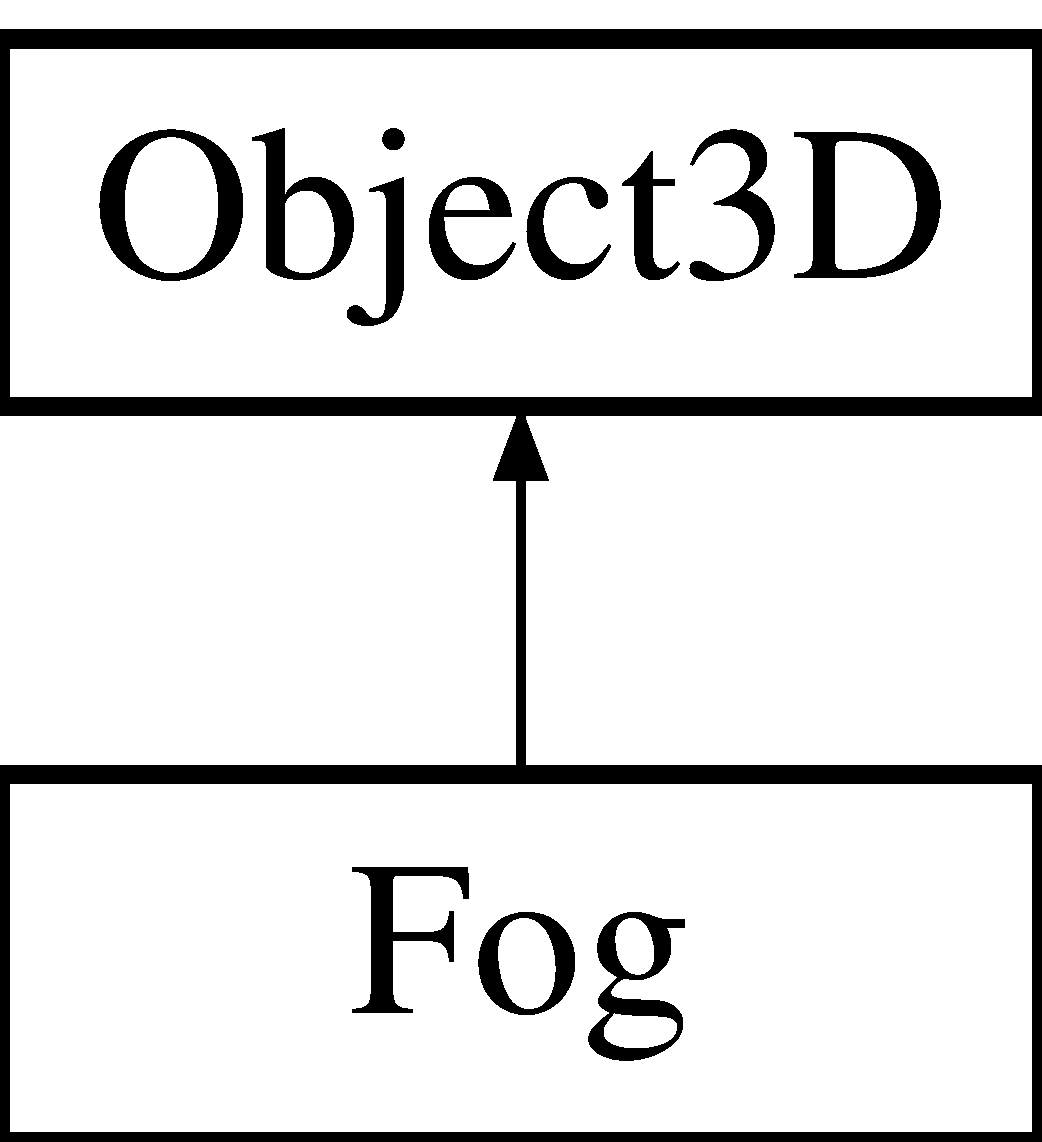
\includegraphics[height=3cm]{classm3g_1_1Fog}
\end{center}
\end{figure}
\subsection*{構成}
\begin{CompactItemize}
\item 
struct \textbf{Distance}
\end{CompactItemize}
\subsection*{Public メソッド}
\begin{CompactItemize}
\item 
\hyperlink{classm3g_1_1Fog_232ea9c5f5824d924fa185401fbfb234}{Fog} ()
\item 
virtual \hyperlink{classm3g_1_1Fog_c13d77e65284ed8f7480c8f83ed9780f}{$\sim$Fog} ()
\item 
virtual \hyperlink{classm3g_1_1Fog}{Fog} $\ast$ \hyperlink{classm3g_1_1Fog_d46dc959a547ee3a804fc871b83c0bbf}{duplicate} () const 
\item 
virtual void \hyperlink{classm3g_1_1Fog_415c0b110f95410ded9b85e5d99a496b}{addAnimationTrack} (\hyperlink{classm3g_1_1AnimationTrack}{AnimationTrack} $\ast$animation\_\-track)
\item 
virtual int \hyperlink{classm3g_1_1Fog_8aad1ceab4c2a03609c8a42324ce484d}{animate} (int world\_\-time)
\item 
int \hyperlink{classm3g_1_1Fog_4cfa1931c265ec3412fe3f6408a1b4f5}{getColor} () const 
\item 
float \hyperlink{classm3g_1_1Fog_31deef556a6aa5e519d3c79bd9c383c0}{getDensity} () const 
\item 
float \hyperlink{classm3g_1_1Fog_90df17252a921929fce6a5e92aed4021}{getFarDistance} () const 
\item 
int \hyperlink{classm3g_1_1Fog_d4ce4524e4751fe5e3cfb8c270347d54}{getMode} () const 
\item 
float \hyperlink{classm3g_1_1Fog_cd7a642e43bf99b0e1c5c24d3c6424a2}{getNearDistance} () const 
\item 
void \hyperlink{classm3g_1_1Fog_b1f5cc0f5cc6bbbd716a526c61f1081d}{setColor} (int rgb)
\item 
void \hyperlink{classm3g_1_1Fog_0ceeda25e326e99d6e971e980a00bd49}{setDensity} (float density)
\item 
void \hyperlink{classm3g_1_1Fog_a46fd556865ae7f1c683c3741b68c168}{setLinear} (float near, float far)
\item 
void \hyperlink{classm3g_1_1Fog_9f407b18ba6235cb96fa95611c1ea3a4}{setMode} (int mode)
\item 
virtual std::ostream \& \hyperlink{classm3g_1_1Fog_6fea17fa1532df3794f8cb39cb4f911f}{print} (std::ostream \&out) const 
\item 
virtual void \hyperlink{classm3g_1_1Fog_8babc8a79b78615da51161e94029eea9}{render} (\hyperlink{structm3g_1_1RenderState}{RenderState} \&state) const 
\end{CompactItemize}
\subsection*{Static Public メソッド}
\begin{CompactItemize}
\item 
static void \hyperlink{classm3g_1_1Fog_443a7a301f77f625335ecc06d13bad06}{renderX} ()
\end{CompactItemize}
\subsection*{Static Public 変数}
\begin{CompactItemize}
\item 
static const int \hyperlink{classm3g_1_1Fog_86b391da2e58c0448712a10f6609a62c}{EXPONENTIAL} = 80
\item 
static const int \hyperlink{classm3g_1_1Fog_23ccf193c67257f1be26417041cecb31}{LINEAR} = 81
\end{CompactItemize}


\subsection{説明}
フォグ属性を内包するアピアランスの構成要素. 

\subsection{コンストラクタとデストラクタ}
\hypertarget{classm3g_1_1Fog_232ea9c5f5824d924fa185401fbfb234}{
\index{m3g::Fog@{m3g::Fog}!Fog@{Fog}}
\index{Fog@{Fog}!m3g::Fog@{m3g::Fog}}
\subsubsection[{Fog}]{\setlength{\rightskip}{0pt plus 5cm}{\bf Fog} ()}}
\label{classm3g_1_1Fog_232ea9c5f5824d924fa185401fbfb234}


新しいFogオブジェクトを作成するコンストラクタ. \hypertarget{classm3g_1_1Fog_c13d77e65284ed8f7480c8f83ed9780f}{
\index{m3g::Fog@{m3g::Fog}!$\sim$Fog@{$\sim$Fog}}
\index{$\sim$Fog@{$\sim$Fog}!m3g::Fog@{m3g::Fog}}
\subsubsection[{$\sim$Fog}]{\setlength{\rightskip}{0pt plus 5cm}$\sim${\bf Fog} ()\hspace{0.3cm}{\tt  \mbox{[}virtual\mbox{]}}}}
\label{classm3g_1_1Fog_c13d77e65284ed8f7480c8f83ed9780f}


このオブジェクトを削除するデストラクタ. 

\subsection{関数}
\hypertarget{classm3g_1_1Fog_415c0b110f95410ded9b85e5d99a496b}{
\index{m3g::Fog@{m3g::Fog}!addAnimationTrack@{addAnimationTrack}}
\index{addAnimationTrack@{addAnimationTrack}!m3g::Fog@{m3g::Fog}}
\subsubsection[{addAnimationTrack}]{\setlength{\rightskip}{0pt plus 5cm}void addAnimationTrack ({\bf AnimationTrack} $\ast$ {\em animation\_\-track})\hspace{0.3cm}{\tt  \mbox{[}virtual\mbox{]}}}}
\label{classm3g_1_1Fog_415c0b110f95410ded9b85e5d99a496b}


アニメーショントラックの追加。 既存のトラックの順番とインデックスは変更されるかもしれない. 

\hyperlink{classm3g_1_1Object3D_415c0b110f95410ded9b85e5d99a496b}{Object3D}を再定義しています。\hypertarget{classm3g_1_1Fog_8aad1ceab4c2a03609c8a42324ce484d}{
\index{m3g::Fog@{m3g::Fog}!animate@{animate}}
\index{animate@{animate}!m3g::Fog@{m3g::Fog}}
\subsubsection[{animate}]{\setlength{\rightskip}{0pt plus 5cm}int animate (int {\em world\_\-time})\hspace{0.3cm}{\tt  \mbox{[}virtual\mbox{]}}}}
\label{classm3g_1_1Fog_8aad1ceab4c2a03609c8a42324ce484d}


アニメーションの更新. 

\hyperlink{classm3g_1_1Object3D_8aad1ceab4c2a03609c8a42324ce484d}{Object3D}を再定義しています。\hypertarget{classm3g_1_1Fog_d46dc959a547ee3a804fc871b83c0bbf}{
\index{m3g::Fog@{m3g::Fog}!duplicate@{duplicate}}
\index{duplicate@{duplicate}!m3g::Fog@{m3g::Fog}}
\subsubsection[{duplicate}]{\setlength{\rightskip}{0pt plus 5cm}{\bf Fog} $\ast$ duplicate () const\hspace{0.3cm}{\tt  \mbox{[}virtual\mbox{]}}}}
\label{classm3g_1_1Fog_d46dc959a547ee3a804fc871b83c0bbf}


このオブジェクトの複製の作成. 

\hyperlink{classm3g_1_1Object3D_a25110dac934f867b83b73ad4741a0f4}{Object3D}を再定義しています。\hypertarget{classm3g_1_1Fog_4cfa1931c265ec3412fe3f6408a1b4f5}{
\index{m3g::Fog@{m3g::Fog}!getColor@{getColor}}
\index{getColor@{getColor}!m3g::Fog@{m3g::Fog}}
\subsubsection[{getColor}]{\setlength{\rightskip}{0pt plus 5cm}int getColor () const}}
\label{classm3g_1_1Fog_4cfa1931c265ec3412fe3f6408a1b4f5}


フォグカラーの取得. \hypertarget{classm3g_1_1Fog_31deef556a6aa5e519d3c79bd9c383c0}{
\index{m3g::Fog@{m3g::Fog}!getDensity@{getDensity}}
\index{getDensity@{getDensity}!m3g::Fog@{m3g::Fog}}
\subsubsection[{getDensity}]{\setlength{\rightskip}{0pt plus 5cm}float getDensity () const}}
\label{classm3g_1_1Fog_31deef556a6aa5e519d3c79bd9c383c0}


フォグ密度の取得. \hypertarget{classm3g_1_1Fog_90df17252a921929fce6a5e92aed4021}{
\index{m3g::Fog@{m3g::Fog}!getFarDistance@{getFarDistance}}
\index{getFarDistance@{getFarDistance}!m3g::Fog@{m3g::Fog}}
\subsubsection[{getFarDistance}]{\setlength{\rightskip}{0pt plus 5cm}float getFarDistance () const}}
\label{classm3g_1_1Fog_90df17252a921929fce6a5e92aed4021}


線形フォグのFar距離の取得. \hypertarget{classm3g_1_1Fog_d4ce4524e4751fe5e3cfb8c270347d54}{
\index{m3g::Fog@{m3g::Fog}!getMode@{getMode}}
\index{getMode@{getMode}!m3g::Fog@{m3g::Fog}}
\subsubsection[{getMode}]{\setlength{\rightskip}{0pt plus 5cm}int getMode () const}}
\label{classm3g_1_1Fog_d4ce4524e4751fe5e3cfb8c270347d54}


カレンドのフォグモードの取得. \hypertarget{classm3g_1_1Fog_cd7a642e43bf99b0e1c5c24d3c6424a2}{
\index{m3g::Fog@{m3g::Fog}!getNearDistance@{getNearDistance}}
\index{getNearDistance@{getNearDistance}!m3g::Fog@{m3g::Fog}}
\subsubsection[{getNearDistance}]{\setlength{\rightskip}{0pt plus 5cm}float getNearDistance () const}}
\label{classm3g_1_1Fog_cd7a642e43bf99b0e1c5c24d3c6424a2}


線形フォグのnear距離の取得. \hypertarget{classm3g_1_1Fog_6fea17fa1532df3794f8cb39cb4f911f}{
\index{m3g::Fog@{m3g::Fog}!print@{print}}
\index{print@{print}!m3g::Fog@{m3g::Fog}}
\subsubsection[{print}]{\setlength{\rightskip}{0pt plus 5cm}std::ostream \& print (std::ostream \& {\em out}) const\hspace{0.3cm}{\tt  \mbox{[}virtual\mbox{]}}}}
\label{classm3g_1_1Fog_6fea17fa1532df3794f8cb39cb4f911f}


このFogクラスの情報を表示する。デバッグ用. 

\hyperlink{classm3g_1_1Object3D_6fea17fa1532df3794f8cb39cb4f911f}{Object3D}を再定義しています。\hypertarget{classm3g_1_1Fog_8babc8a79b78615da51161e94029eea9}{
\index{m3g::Fog@{m3g::Fog}!render@{render}}
\index{render@{render}!m3g::Fog@{m3g::Fog}}
\subsubsection[{render}]{\setlength{\rightskip}{0pt plus 5cm}void render ({\bf RenderState} \& {\em state}) const\hspace{0.3cm}{\tt  \mbox{[}virtual\mbox{]}}}}
\label{classm3g_1_1Fog_8babc8a79b78615da51161e94029eea9}


このFogノードをレンダリングする内部使用の関数.

Note: \hyperlink{classm3g_1_1Fog}{Fog} should be rendered only at second rendering pass(pass=2). In other cases, do nothing. 

\hyperlink{classm3g_1_1Object3D_8babc8a79b78615da51161e94029eea9}{Object3D}を再定義しています。\hypertarget{classm3g_1_1Fog_443a7a301f77f625335ecc06d13bad06}{
\index{m3g::Fog@{m3g::Fog}!renderX@{renderX}}
\index{renderX@{renderX}!m3g::Fog@{m3g::Fog}}
\subsubsection[{renderX}]{\setlength{\rightskip}{0pt plus 5cm}void renderX ()\hspace{0.3cm}{\tt  \mbox{[}static\mbox{]}}}}
\label{classm3g_1_1Fog_443a7a301f77f625335ecc06d13bad06}


デフォルト値でレンダリングする内部使用の関数. \hypertarget{classm3g_1_1Fog_b1f5cc0f5cc6bbbd716a526c61f1081d}{
\index{m3g::Fog@{m3g::Fog}!setColor@{setColor}}
\index{setColor@{setColor}!m3g::Fog@{m3g::Fog}}
\subsubsection[{setColor}]{\setlength{\rightskip}{0pt plus 5cm}void setColor (int {\em rgb})}}
\label{classm3g_1_1Fog_b1f5cc0f5cc6bbbd716a526c61f1081d}


このフォグのカラーの設定. \hypertarget{classm3g_1_1Fog_0ceeda25e326e99d6e971e980a00bd49}{
\index{m3g::Fog@{m3g::Fog}!setDensity@{setDensity}}
\index{setDensity@{setDensity}!m3g::Fog@{m3g::Fog}}
\subsubsection[{setDensity}]{\setlength{\rightskip}{0pt plus 5cm}void setDensity (float {\em density})}}
\label{classm3g_1_1Fog_0ceeda25e326e99d6e971e980a00bd49}


フォグの指数密度の設定. \hypertarget{classm3g_1_1Fog_a46fd556865ae7f1c683c3741b68c168}{
\index{m3g::Fog@{m3g::Fog}!setLinear@{setLinear}}
\index{setLinear@{setLinear}!m3g::Fog@{m3g::Fog}}
\subsubsection[{setLinear}]{\setlength{\rightskip}{0pt plus 5cm}void setLinear (float {\em near}, \/  float {\em far})}}
\label{classm3g_1_1Fog_a46fd556865ae7f1c683c3741b68c168}


線形フォグのnear,far距離の設定. \hypertarget{classm3g_1_1Fog_9f407b18ba6235cb96fa95611c1ea3a4}{
\index{m3g::Fog@{m3g::Fog}!setMode@{setMode}}
\index{setMode@{setMode}!m3g::Fog@{m3g::Fog}}
\subsubsection[{setMode}]{\setlength{\rightskip}{0pt plus 5cm}void setMode (int {\em mode})}}
\label{classm3g_1_1Fog_9f407b18ba6235cb96fa95611c1ea3a4}


フォグモードを線形もしくはexponentialに設定する. 

\subsection{変数}
\hypertarget{classm3g_1_1Fog_86b391da2e58c0448712a10f6609a62c}{
\index{m3g::Fog@{m3g::Fog}!EXPONENTIAL@{EXPONENTIAL}}
\index{EXPONENTIAL@{EXPONENTIAL}!m3g::Fog@{m3g::Fog}}
\subsubsection[{EXPONENTIAL}]{\setlength{\rightskip}{0pt plus 5cm}const int {\bf EXPONENTIAL} = 80\hspace{0.3cm}{\tt  \mbox{[}static\mbox{]}}}}
\label{classm3g_1_1Fog_86b391da2e58c0448712a10f6609a62c}


指数フォグを表す定数. \hypertarget{classm3g_1_1Fog_23ccf193c67257f1be26417041cecb31}{
\index{m3g::Fog@{m3g::Fog}!LINEAR@{LINEAR}}
\index{LINEAR@{LINEAR}!m3g::Fog@{m3g::Fog}}
\subsubsection[{LINEAR}]{\setlength{\rightskip}{0pt plus 5cm}const int {\bf LINEAR} = 81\hspace{0.3cm}{\tt  \mbox{[}static\mbox{]}}}}
\label{classm3g_1_1Fog_23ccf193c67257f1be26417041cecb31}


線形フォグを表す定数. 

このクラスの説明は次のファイルから生成されました:\begin{CompactItemize}
\item 
/work/workspace.desktop-m3g/src/Fog.hpp\item 
/work/workspace.desktop-m3g/src/Fog.cpp\end{CompactItemize}

\hypertarget{classm3g_1_1Graphics}{
\section{クラス Graphics}
\label{classm3g_1_1Graphics}\index{m3g::Graphics@{m3g::Graphics}}
}
{\tt \#include $<$Graphics.hpp$>$}



\subsection{説明}
JAVAのGraphicsクラスに相当するダミークラス。C/C++およびRubyでは何も行わない. 

このクラスの説明は次のファイルから生成されました:\begin{CompactItemize}
\item 
/work/desktop-m3g/src/Graphics.hpp\end{CompactItemize}

\hypertarget{classm3g_1_1Graphics3D}{
\section{Graphics3D Class Reference}
\label{classm3g_1_1Graphics3D}\index{m3g::Graphics3D@{m3g::Graphics3D}}
}
{\tt \#include $<$Graphics3D.hpp$>$}

Inheritance diagram for Graphics3D::\begin{figure}[H]
\begin{center}
\leavevmode
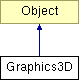
\includegraphics[height=2cm]{classm3g_1_1Graphics3D}
\end{center}
\end{figure}
\subsection*{Classes}
\begin{CompactItemize}
\item 
struct \textbf{Viewport}
\end{CompactItemize}
\subsection*{Public Member Functions}
\begin{CompactItemize}
\item 
\hyperlink{classm3g_1_1Graphics3D_9b9347476fc10e57b31694ac8a628511}{$\sim$Graphics3D} ()
\item 
int \hyperlink{classm3g_1_1Graphics3D_0a8acc61618bad17053cb62131819b92}{addLight} (\hyperlink{classm3g_1_1Light}{Light} $\ast$light, const \hyperlink{classm3g_1_1Transform}{Transform} \&transform)
\item 
void \hyperlink{classm3g_1_1Graphics3D_d34fb1ab11f2e25b98b93affd71dcc05}{bindTarget} (void $\ast$target, bool depth\_\-buffer\_\-enabled=true, int hints=0)
\item 
void \hyperlink{classm3g_1_1Graphics3D_b775163cbe39d177e255011e381cd9f8}{bindTarget} (\hyperlink{classm3g_1_1Image2D}{Image2D} $\ast$target, bool depth\_\-buffer\_\-enabled=true, int hints=0)
\item 
void \hyperlink{classm3g_1_1Graphics3D_21c4a68a53cfbe0a7cec05d5a56682bf}{clear} (\hyperlink{classm3g_1_1Background}{Background} $\ast$background)
\item 
\hyperlink{classm3g_1_1Camera}{Camera} $\ast$ \hyperlink{classm3g_1_1Graphics3D_1c6ba79e9112caef92e1a149a308b613}{getCamera} (\hyperlink{classm3g_1_1Transform}{Transform} $\ast$transform)
\item 
float \hyperlink{classm3g_1_1Graphics3D_c8c185b99073215202d2e35723f5c470}{getDepthRangeFar} () const 
\item 
float \hyperlink{classm3g_1_1Graphics3D_60bc116f673bf2782de2df3eebfb2c92}{getDepthRangeNear} () const 
\item 
int \hyperlink{classm3g_1_1Graphics3D_5837234a23dc5f46d3adec17f521b58e}{getHints} () const 
\item 
\hyperlink{classm3g_1_1Light}{Light} $\ast$ \hyperlink{classm3g_1_1Graphics3D_02e7b19ae5c0342b11f2cbf9a4df4d77}{getLight} (int index, \hyperlink{classm3g_1_1Transform}{Transform} $\ast$transform) const 
\item 
int \hyperlink{classm3g_1_1Graphics3D_7a08cfeb48d76ad5d8859a1fc0c77d98}{getLightCount} () const 
\item 
std::map$<$ const char $\ast$, int $>$ \hyperlink{classm3g_1_1Graphics3D_2ea2a069c4b10555d50a193a44e63996}{getProperties} () const 
\item 
void $\ast$ \hyperlink{classm3g_1_1Graphics3D_02d0033930c8e68f4d7ebd43abe7980a}{getTarget} () const 
\item 
int \hyperlink{classm3g_1_1Graphics3D_d51e0c421126f5deb61b359cdb7dab2e}{getViewportHeight} () const 
\item 
int \hyperlink{classm3g_1_1Graphics3D_768e5c057e2fa4c4b17a67134abbf89f}{getViewportWidth} () const 
\item 
int \hyperlink{classm3g_1_1Graphics3D_af58b44cc6219f86c40dadb8a9377856}{getViewportX} () const 
\item 
int \hyperlink{classm3g_1_1Graphics3D_c21665afbf94a8f0153e099833c2b61a}{getViewportY} () const 
\item 
bool \hyperlink{classm3g_1_1Graphics3D_7f17c6781152840d42e756c27b0fb8c8}{isDepthBufferEnabled} () const 
\item 
void \hyperlink{classm3g_1_1Graphics3D_1491a435e97a20d5325339359a719cc5}{releaseTarget} ()
\item 
void \hyperlink{classm3g_1_1Graphics3D_8f7b52c44e84e6ccbbb639d1b5b80466}{render} (\hyperlink{classm3g_1_1Node}{Node} $\ast$node, const \hyperlink{classm3g_1_1Transform}{Transform} \&transform) const 
\item 
void \hyperlink{classm3g_1_1Graphics3D_c809eea19f3eaff279628081fc90cf36}{render} (\hyperlink{classm3g_1_1VertexBuffer}{VertexBuffer} $\ast$vertices, \hyperlink{classm3g_1_1IndexBuffer}{IndexBuffer} $\ast$triangles, \hyperlink{classm3g_1_1Appearance}{Appearance} $\ast$apperance, \hyperlink{classm3g_1_1Transform}{Transform} \&transform, int scope=-1) const 
\item 
void \hyperlink{classm3g_1_1Graphics3D_8ef004c92d601203b8c697d441e7713f}{render} (\hyperlink{classm3g_1_1World}{World} $\ast$world) const 
\item 
void \hyperlink{classm3g_1_1Graphics3D_b8821ec231e8ebd939ae0feaaf138542}{resetLights} ()
\item 
void \hyperlink{classm3g_1_1Graphics3D_0df7bb61cfeba6626e20fd07ddd1c460}{setCamera} (\hyperlink{classm3g_1_1Camera}{Camera} $\ast$camera, const \hyperlink{classm3g_1_1Transform}{Transform} \&transform)
\item 
void \hyperlink{classm3g_1_1Graphics3D_6fc3837286f3516aa3320aeec9729495}{setDepthRange} (float near, float far)
\item 
void \hyperlink{classm3g_1_1Graphics3D_2bf83cb69f50117dd9d5548fe96d0ab0}{setLight} (int index, \hyperlink{classm3g_1_1Light}{Light} $\ast$light, const \hyperlink{classm3g_1_1Transform}{Transform} \&transform)
\item 
void \hyperlink{classm3g_1_1Graphics3D_0b4ec48e9c19060e9be5648c118c23b1}{setViewport} (int x, int y, int width, int height)
\item 
std::ostream \& \hyperlink{classm3g_1_1Graphics3D_6fea17fa1532df3794f8cb39cb4f911f}{print} (std::ostream \&out) const 
\end{CompactItemize}
\subsection*{Static Public Member Functions}
\begin{CompactItemize}
\item 
static \hyperlink{classm3g_1_1Graphics3D}{Graphics3D} $\ast$ \hyperlink{classm3g_1_1Graphics3D_da6d71754bfe755dd8204a9332e9ed47}{getInstance} ()
\end{CompactItemize}
\subsection*{Static Public Attributes}
\begin{CompactItemize}
\item 
\hypertarget{classm3g_1_1Graphics3D_9df12c5332904e66a962e1bf2809a812}{
static const int \textbf{ANTIALIAS} = 1$<$$<$1}
\label{classm3g_1_1Graphics3D_9df12c5332904e66a962e1bf2809a812}

\item 
\hypertarget{classm3g_1_1Graphics3D_3750f57b82328be988bdab3b672a64f9}{
static const int \textbf{DITHER} = 1$<$$<$2}
\label{classm3g_1_1Graphics3D_3750f57b82328be988bdab3b672a64f9}

\item 
\hypertarget{classm3g_1_1Graphics3D_f448f7f447a301823af9170bfe84c50e}{
static const int \textbf{OVERWRITE} = 1$<$$<$4}
\label{classm3g_1_1Graphics3D_f448f7f447a301823af9170bfe84c50e}

\item 
\hypertarget{classm3g_1_1Graphics3D_bbd22a6baea672f895d5ef32e2438ec6}{
static const int \textbf{TRUE\_\-COLOR} = 1$<$$<$3}
\label{classm3g_1_1Graphics3D_bbd22a6baea672f895d5ef32e2438ec6}

\item 
\hypertarget{classm3g_1_1Graphics3D_6b0cb63f7c2814ea8c1938d1b9c50cfa}{
static const int \textbf{TARGET\_\-NONE} = 0}
\label{classm3g_1_1Graphics3D_6b0cb63f7c2814ea8c1938d1b9c50cfa}

\item 
\hypertarget{classm3g_1_1Graphics3D_84569f5576be7f299b00c6de2ba775d0}{
static const int \textbf{TARGET\_\-DEFAULT} = 1}
\label{classm3g_1_1Graphics3D_84569f5576be7f299b00c6de2ba775d0}

\item 
\hypertarget{classm3g_1_1Graphics3D_75fa6b63c910b61d5d3ec8c419d75ec2}{
static const int \textbf{TARGET\_\-IMAGE2D} = 2}
\label{classm3g_1_1Graphics3D_75fa6b63c910b61d5d3ec8c419d75ec2}

\end{CompactItemize}


\subsection{Detailed Description}
A singleton 3D graphics context that can be bound to a rendering target. 

\subsection{Constructor \& Destructor Documentation}
\hypertarget{classm3g_1_1Graphics3D_9b9347476fc10e57b31694ac8a628511}{
\index{m3g::Graphics3D@{m3g::Graphics3D}!$\sim$Graphics3D@{$\sim$Graphics3D}}
\index{$\sim$Graphics3D@{$\sim$Graphics3D}!m3g::Graphics3D@{m3g::Graphics3D}}
\subsubsection[{$\sim$Graphics3D}]{\setlength{\rightskip}{0pt plus 5cm}$\sim${\bf Graphics3D} ()}}
\label{classm3g_1_1Graphics3D_9b9347476fc10e57b31694ac8a628511}


Destruct this object. 

\subsection{Member Function Documentation}
\hypertarget{classm3g_1_1Graphics3D_0a8acc61618bad17053cb62131819b92}{
\index{m3g::Graphics3D@{m3g::Graphics3D}!addLight@{addLight}}
\index{addLight@{addLight}!m3g::Graphics3D@{m3g::Graphics3D}}
\subsubsection[{addLight}]{\setlength{\rightskip}{0pt plus 5cm}int addLight ({\bf Light} $\ast$ {\em light}, \/  const {\bf Transform} \& {\em transform})}}
\label{classm3g_1_1Graphics3D_0a8acc61618bad17053cb62131819b92}


Binds a \hyperlink{classm3g_1_1Light}{Light} to use in subsequent immediate mode rendering. \hypertarget{classm3g_1_1Graphics3D_b775163cbe39d177e255011e381cd9f8}{
\index{m3g::Graphics3D@{m3g::Graphics3D}!bindTarget@{bindTarget}}
\index{bindTarget@{bindTarget}!m3g::Graphics3D@{m3g::Graphics3D}}
\subsubsection[{bindTarget}]{\setlength{\rightskip}{0pt plus 5cm}void bindTarget ({\bf Image2D} $\ast$ {\em target}, \/  bool {\em depth\_\-buffer\_\-enabled} = {\tt true}, \/  int {\em hints} = {\tt 0})}}
\label{classm3g_1_1Graphics3D_b775163cbe39d177e255011e381cd9f8}


Binds mutable Image 2D as the rendring ttarget of this \hyperlink{classm3g_1_1Graphics3D}{Graphics3D}. \hypertarget{classm3g_1_1Graphics3D_d34fb1ab11f2e25b98b93affd71dcc05}{
\index{m3g::Graphics3D@{m3g::Graphics3D}!bindTarget@{bindTarget}}
\index{bindTarget@{bindTarget}!m3g::Graphics3D@{m3g::Graphics3D}}
\subsubsection[{bindTarget}]{\setlength{\rightskip}{0pt plus 5cm}void bindTarget (void $\ast$ {\em target}, \/  bool {\em depth\_\-buffer\_\-enabled} = {\tt true}, \/  int {\em hints} = {\tt 0})}}
\label{classm3g_1_1Graphics3D_d34fb1ab11f2e25b98b93affd71dcc05}


Binds the defualt (frame buffer) as the rendring ttarget of this \hyperlink{classm3g_1_1Graphics3D}{Graphics3D}. \hypertarget{classm3g_1_1Graphics3D_21c4a68a53cfbe0a7cec05d5a56682bf}{
\index{m3g::Graphics3D@{m3g::Graphics3D}!clear@{clear}}
\index{clear@{clear}!m3g::Graphics3D@{m3g::Graphics3D}}
\subsubsection[{clear}]{\setlength{\rightskip}{0pt plus 5cm}void clear ({\bf Background} $\ast$ {\em background})}}
\label{classm3g_1_1Graphics3D_21c4a68a53cfbe0a7cec05d5a56682bf}


Clears the viewport as specified in the given \hyperlink{classm3g_1_1Background}{Background} object. \hypertarget{classm3g_1_1Graphics3D_1c6ba79e9112caef92e1a149a308b613}{
\index{m3g::Graphics3D@{m3g::Graphics3D}!getCamera@{getCamera}}
\index{getCamera@{getCamera}!m3g::Graphics3D@{m3g::Graphics3D}}
\subsubsection[{getCamera}]{\setlength{\rightskip}{0pt plus 5cm}{\bf Camera} $\ast$ getCamera ({\bf Transform} $\ast$ {\em transform})}}
\label{classm3g_1_1Graphics3D_1c6ba79e9112caef92e1a149a308b613}


Returns the current camera. \hypertarget{classm3g_1_1Graphics3D_c8c185b99073215202d2e35723f5c470}{
\index{m3g::Graphics3D@{m3g::Graphics3D}!getDepthRangeFar@{getDepthRangeFar}}
\index{getDepthRangeFar@{getDepthRangeFar}!m3g::Graphics3D@{m3g::Graphics3D}}
\subsubsection[{getDepthRangeFar}]{\setlength{\rightskip}{0pt plus 5cm}float getDepthRangeFar () const}}
\label{classm3g_1_1Graphics3D_c8c185b99073215202d2e35723f5c470}


Returns the far distance of the depth range. \hypertarget{classm3g_1_1Graphics3D_60bc116f673bf2782de2df3eebfb2c92}{
\index{m3g::Graphics3D@{m3g::Graphics3D}!getDepthRangeNear@{getDepthRangeNear}}
\index{getDepthRangeNear@{getDepthRangeNear}!m3g::Graphics3D@{m3g::Graphics3D}}
\subsubsection[{getDepthRangeNear}]{\setlength{\rightskip}{0pt plus 5cm}float getDepthRangeNear () const}}
\label{classm3g_1_1Graphics3D_60bc116f673bf2782de2df3eebfb2c92}


Returns the near distance of the depth range. \hypertarget{classm3g_1_1Graphics3D_5837234a23dc5f46d3adec17f521b58e}{
\index{m3g::Graphics3D@{m3g::Graphics3D}!getHints@{getHints}}
\index{getHints@{getHints}!m3g::Graphics3D@{m3g::Graphics3D}}
\subsubsection[{getHints}]{\setlength{\rightskip}{0pt plus 5cm}int getHints () const}}
\label{classm3g_1_1Graphics3D_5837234a23dc5f46d3adec17f521b58e}


Returns the rendering hints given for the current rendering target. \hypertarget{classm3g_1_1Graphics3D_da6d71754bfe755dd8204a9332e9ed47}{
\index{m3g::Graphics3D@{m3g::Graphics3D}!getInstance@{getInstance}}
\index{getInstance@{getInstance}!m3g::Graphics3D@{m3g::Graphics3D}}
\subsubsection[{getInstance}]{\setlength{\rightskip}{0pt plus 5cm}{\bf Graphics3D} $\ast$ getInstance ()\hspace{0.3cm}{\tt  \mbox{[}static\mbox{]}}}}
\label{classm3g_1_1Graphics3D_da6d71754bfe755dd8204a9332e9ed47}


Retrieves the singleton \hyperlink{classm3g_1_1Graphics3D}{Graphics3D} instance that is associated with this application. \hypertarget{classm3g_1_1Graphics3D_02e7b19ae5c0342b11f2cbf9a4df4d77}{
\index{m3g::Graphics3D@{m3g::Graphics3D}!getLight@{getLight}}
\index{getLight@{getLight}!m3g::Graphics3D@{m3g::Graphics3D}}
\subsubsection[{getLight}]{\setlength{\rightskip}{0pt plus 5cm}{\bf Light} $\ast$ getLight (int {\em index}, \/  {\bf Transform} $\ast$ {\em transform}) const}}
\label{classm3g_1_1Graphics3D_02e7b19ae5c0342b11f2cbf9a4df4d77}


Returns a light int he current light array. \hypertarget{classm3g_1_1Graphics3D_7a08cfeb48d76ad5d8859a1fc0c77d98}{
\index{m3g::Graphics3D@{m3g::Graphics3D}!getLightCount@{getLightCount}}
\index{getLightCount@{getLightCount}!m3g::Graphics3D@{m3g::Graphics3D}}
\subsubsection[{getLightCount}]{\setlength{\rightskip}{0pt plus 5cm}int getLightCount () const}}
\label{classm3g_1_1Graphics3D_7a08cfeb48d76ad5d8859a1fc0c77d98}


Returns the size of the current light array. \hypertarget{classm3g_1_1Graphics3D_2ea2a069c4b10555d50a193a44e63996}{
\index{m3g::Graphics3D@{m3g::Graphics3D}!getProperties@{getProperties}}
\index{getProperties@{getProperties}!m3g::Graphics3D@{m3g::Graphics3D}}
\subsubsection[{getProperties}]{\setlength{\rightskip}{0pt plus 5cm}std::map$<$ const char $\ast$, int $>$ getProperties () const}}
\label{classm3g_1_1Graphics3D_2ea2a069c4b10555d50a193a44e63996}


Retrieves implementation specific peoperties. \hypertarget{classm3g_1_1Graphics3D_02d0033930c8e68f4d7ebd43abe7980a}{
\index{m3g::Graphics3D@{m3g::Graphics3D}!getTarget@{getTarget}}
\index{getTarget@{getTarget}!m3g::Graphics3D@{m3g::Graphics3D}}
\subsubsection[{getTarget}]{\setlength{\rightskip}{0pt plus 5cm}void $\ast$ getTarget () const}}
\label{classm3g_1_1Graphics3D_02d0033930c8e68f4d7ebd43abe7980a}


Returns the current rendierng target. \hypertarget{classm3g_1_1Graphics3D_d51e0c421126f5deb61b359cdb7dab2e}{
\index{m3g::Graphics3D@{m3g::Graphics3D}!getViewportHeight@{getViewportHeight}}
\index{getViewportHeight@{getViewportHeight}!m3g::Graphics3D@{m3g::Graphics3D}}
\subsubsection[{getViewportHeight}]{\setlength{\rightskip}{0pt plus 5cm}int getViewportHeight () const}}
\label{classm3g_1_1Graphics3D_d51e0c421126f5deb61b359cdb7dab2e}


Returns the height of the viewport. \hypertarget{classm3g_1_1Graphics3D_768e5c057e2fa4c4b17a67134abbf89f}{
\index{m3g::Graphics3D@{m3g::Graphics3D}!getViewportWidth@{getViewportWidth}}
\index{getViewportWidth@{getViewportWidth}!m3g::Graphics3D@{m3g::Graphics3D}}
\subsubsection[{getViewportWidth}]{\setlength{\rightskip}{0pt plus 5cm}int getViewportWidth () const}}
\label{classm3g_1_1Graphics3D_768e5c057e2fa4c4b17a67134abbf89f}


Returns the width of the viewport. \hypertarget{classm3g_1_1Graphics3D_af58b44cc6219f86c40dadb8a9377856}{
\index{m3g::Graphics3D@{m3g::Graphics3D}!getViewportX@{getViewportX}}
\index{getViewportX@{getViewportX}!m3g::Graphics3D@{m3g::Graphics3D}}
\subsubsection[{getViewportX}]{\setlength{\rightskip}{0pt plus 5cm}int getViewportX () const}}
\label{classm3g_1_1Graphics3D_af58b44cc6219f86c40dadb8a9377856}


Returns the horizontal position of the viewport. \hypertarget{classm3g_1_1Graphics3D_c21665afbf94a8f0153e099833c2b61a}{
\index{m3g::Graphics3D@{m3g::Graphics3D}!getViewportY@{getViewportY}}
\index{getViewportY@{getViewportY}!m3g::Graphics3D@{m3g::Graphics3D}}
\subsubsection[{getViewportY}]{\setlength{\rightskip}{0pt plus 5cm}int getViewportY () const}}
\label{classm3g_1_1Graphics3D_c21665afbf94a8f0153e099833c2b61a}


Returns the vertical position of the viewport. \hypertarget{classm3g_1_1Graphics3D_7f17c6781152840d42e756c27b0fb8c8}{
\index{m3g::Graphics3D@{m3g::Graphics3D}!isDepthBufferEnabled@{isDepthBufferEnabled}}
\index{isDepthBufferEnabled@{isDepthBufferEnabled}!m3g::Graphics3D@{m3g::Graphics3D}}
\subsubsection[{isDepthBufferEnabled}]{\setlength{\rightskip}{0pt plus 5cm}bool isDepthBufferEnabled () const}}
\label{classm3g_1_1Graphics3D_7f17c6781152840d42e756c27b0fb8c8}


Queries whether depth buffering is enalbed for the current rendering target. \hypertarget{classm3g_1_1Graphics3D_6fea17fa1532df3794f8cb39cb4f911f}{
\index{m3g::Graphics3D@{m3g::Graphics3D}!print@{print}}
\index{print@{print}!m3g::Graphics3D@{m3g::Graphics3D}}
\subsubsection[{print}]{\setlength{\rightskip}{0pt plus 5cm}std::ostream \& print (std::ostream \& {\em out}) const}}
\label{classm3g_1_1Graphics3D_6fea17fa1532df3794f8cb39cb4f911f}


Print out information of this object, for debug only. 

Reimplemented from \hyperlink{classm3g_1_1Object_6fea17fa1532df3794f8cb39cb4f911f}{Object}.\hypertarget{classm3g_1_1Graphics3D_1491a435e97a20d5325339359a719cc5}{
\index{m3g::Graphics3D@{m3g::Graphics3D}!releaseTarget@{releaseTarget}}
\index{releaseTarget@{releaseTarget}!m3g::Graphics3D@{m3g::Graphics3D}}
\subsubsection[{releaseTarget}]{\setlength{\rightskip}{0pt plus 5cm}void releaseTarget ()}}
\label{classm3g_1_1Graphics3D_1491a435e97a20d5325339359a719cc5}


Flushes the renderd 3D image to the currently bound target and then releases the target. \hypertarget{classm3g_1_1Graphics3D_8ef004c92d601203b8c697d441e7713f}{
\index{m3g::Graphics3D@{m3g::Graphics3D}!render@{render}}
\index{render@{render}!m3g::Graphics3D@{m3g::Graphics3D}}
\subsubsection[{render}]{\setlength{\rightskip}{0pt plus 5cm}void render ({\bf World} $\ast$ {\em world}) const}}
\label{classm3g_1_1Graphics3D_8ef004c92d601203b8c697d441e7713f}


Rnders a image of world as viewd by the active camera of that \hyperlink{classm3g_1_1World}{World}. \hypertarget{classm3g_1_1Graphics3D_c809eea19f3eaff279628081fc90cf36}{
\index{m3g::Graphics3D@{m3g::Graphics3D}!render@{render}}
\index{render@{render}!m3g::Graphics3D@{m3g::Graphics3D}}
\subsubsection[{render}]{\setlength{\rightskip}{0pt plus 5cm}void render ({\bf VertexBuffer} $\ast$ {\em vertices}, \/  {\bf IndexBuffer} $\ast$ {\em triangles}, \/  {\bf Appearance} $\ast$ {\em apperance}, \/  {\bf Transform} \& {\em transform}, \/  int {\em scope} = {\tt -1}) const}}
\label{classm3g_1_1Graphics3D_c809eea19f3eaff279628081fc90cf36}


Renders \hypertarget{classm3g_1_1Graphics3D_8f7b52c44e84e6ccbbb639d1b5b80466}{
\index{m3g::Graphics3D@{m3g::Graphics3D}!render@{render}}
\index{render@{render}!m3g::Graphics3D@{m3g::Graphics3D}}
\subsubsection[{render}]{\setlength{\rightskip}{0pt plus 5cm}void render ({\bf Node} $\ast$ {\em node}, \/  const {\bf Transform} \& {\em transform}) const}}
\label{classm3g_1_1Graphics3D_8f7b52c44e84e6ccbbb639d1b5b80466}


Renders the given \hyperlink{classm3g_1_1Sprite3D}{Sprite3D}, \hyperlink{classm3g_1_1Mesh}{Mesh}, or Group node with the given transformation from local coordinates to world coordinates. \hypertarget{classm3g_1_1Graphics3D_b8821ec231e8ebd939ae0feaaf138542}{
\index{m3g::Graphics3D@{m3g::Graphics3D}!resetLights@{resetLights}}
\index{resetLights@{resetLights}!m3g::Graphics3D@{m3g::Graphics3D}}
\subsubsection[{resetLights}]{\setlength{\rightskip}{0pt plus 5cm}void resetLights ()}}
\label{classm3g_1_1Graphics3D_b8821ec231e8ebd939ae0feaaf138542}


Clears the array of current Lights. \hypertarget{classm3g_1_1Graphics3D_0df7bb61cfeba6626e20fd07ddd1c460}{
\index{m3g::Graphics3D@{m3g::Graphics3D}!setCamera@{setCamera}}
\index{setCamera@{setCamera}!m3g::Graphics3D@{m3g::Graphics3D}}
\subsubsection[{setCamera}]{\setlength{\rightskip}{0pt plus 5cm}void setCamera ({\bf Camera} $\ast$ {\em camera}, \/  const {\bf Transform} \& {\em transform})}}
\label{classm3g_1_1Graphics3D_0df7bb61cfeba6626e20fd07ddd1c460}


Sets the \hyperlink{classm3g_1_1Camera}{Camera} to use in subsequent immediate mode rendering. \hypertarget{classm3g_1_1Graphics3D_6fc3837286f3516aa3320aeec9729495}{
\index{m3g::Graphics3D@{m3g::Graphics3D}!setDepthRange@{setDepthRange}}
\index{setDepthRange@{setDepthRange}!m3g::Graphics3D@{m3g::Graphics3D}}
\subsubsection[{setDepthRange}]{\setlength{\rightskip}{0pt plus 5cm}void setDepthRange (float {\em near}, \/  float {\em far})}}
\label{classm3g_1_1Graphics3D_6fc3837286f3516aa3320aeec9729495}


Specifies the mappin gof depth values from normalized device coordinates to window coordinates. \hypertarget{classm3g_1_1Graphics3D_2bf83cb69f50117dd9d5548fe96d0ab0}{
\index{m3g::Graphics3D@{m3g::Graphics3D}!setLight@{setLight}}
\index{setLight@{setLight}!m3g::Graphics3D@{m3g::Graphics3D}}
\subsubsection[{setLight}]{\setlength{\rightskip}{0pt plus 5cm}void setLight (int {\em index}, \/  {\bf Light} $\ast$ {\em light}, \/  const {\bf Transform} \& {\em transform})}}
\label{classm3g_1_1Graphics3D_2bf83cb69f50117dd9d5548fe96d0ab0}


Replaces or modifies a \hyperlink{classm3g_1_1Light}{Light} currently bound for immediate mode rendering. \hypertarget{classm3g_1_1Graphics3D_0b4ec48e9c19060e9be5648c118c23b1}{
\index{m3g::Graphics3D@{m3g::Graphics3D}!setViewport@{setViewport}}
\index{setViewport@{setViewport}!m3g::Graphics3D@{m3g::Graphics3D}}
\subsubsection[{setViewport}]{\setlength{\rightskip}{0pt plus 5cm}void setViewport (int {\em x}, \/  int {\em y}, \/  int {\em width}, \/  int {\em height})}}
\label{classm3g_1_1Graphics3D_0b4ec48e9c19060e9be5648c118c23b1}


Specifies a rectangular viewport on the currently bound rendering target. 

The documentation for this class was generated from the following files:\begin{CompactItemize}
\item 
/work/workspace.desktop-m3g/src/Graphics3D.hpp\item 
/work/workspace.desktop-m3g/src/Graphics3D.cpp\end{CompactItemize}

\hypertarget{classm3g_1_1Group}{
\section{クラス Group}
\label{classm3g_1_1Group}\index{m3g::Group@{m3g::Group}}
}
{\tt \#include $<$Group.hpp$>$}

Groupに対する継承グラフ:\begin{figure}[H]
\begin{center}
\leavevmode
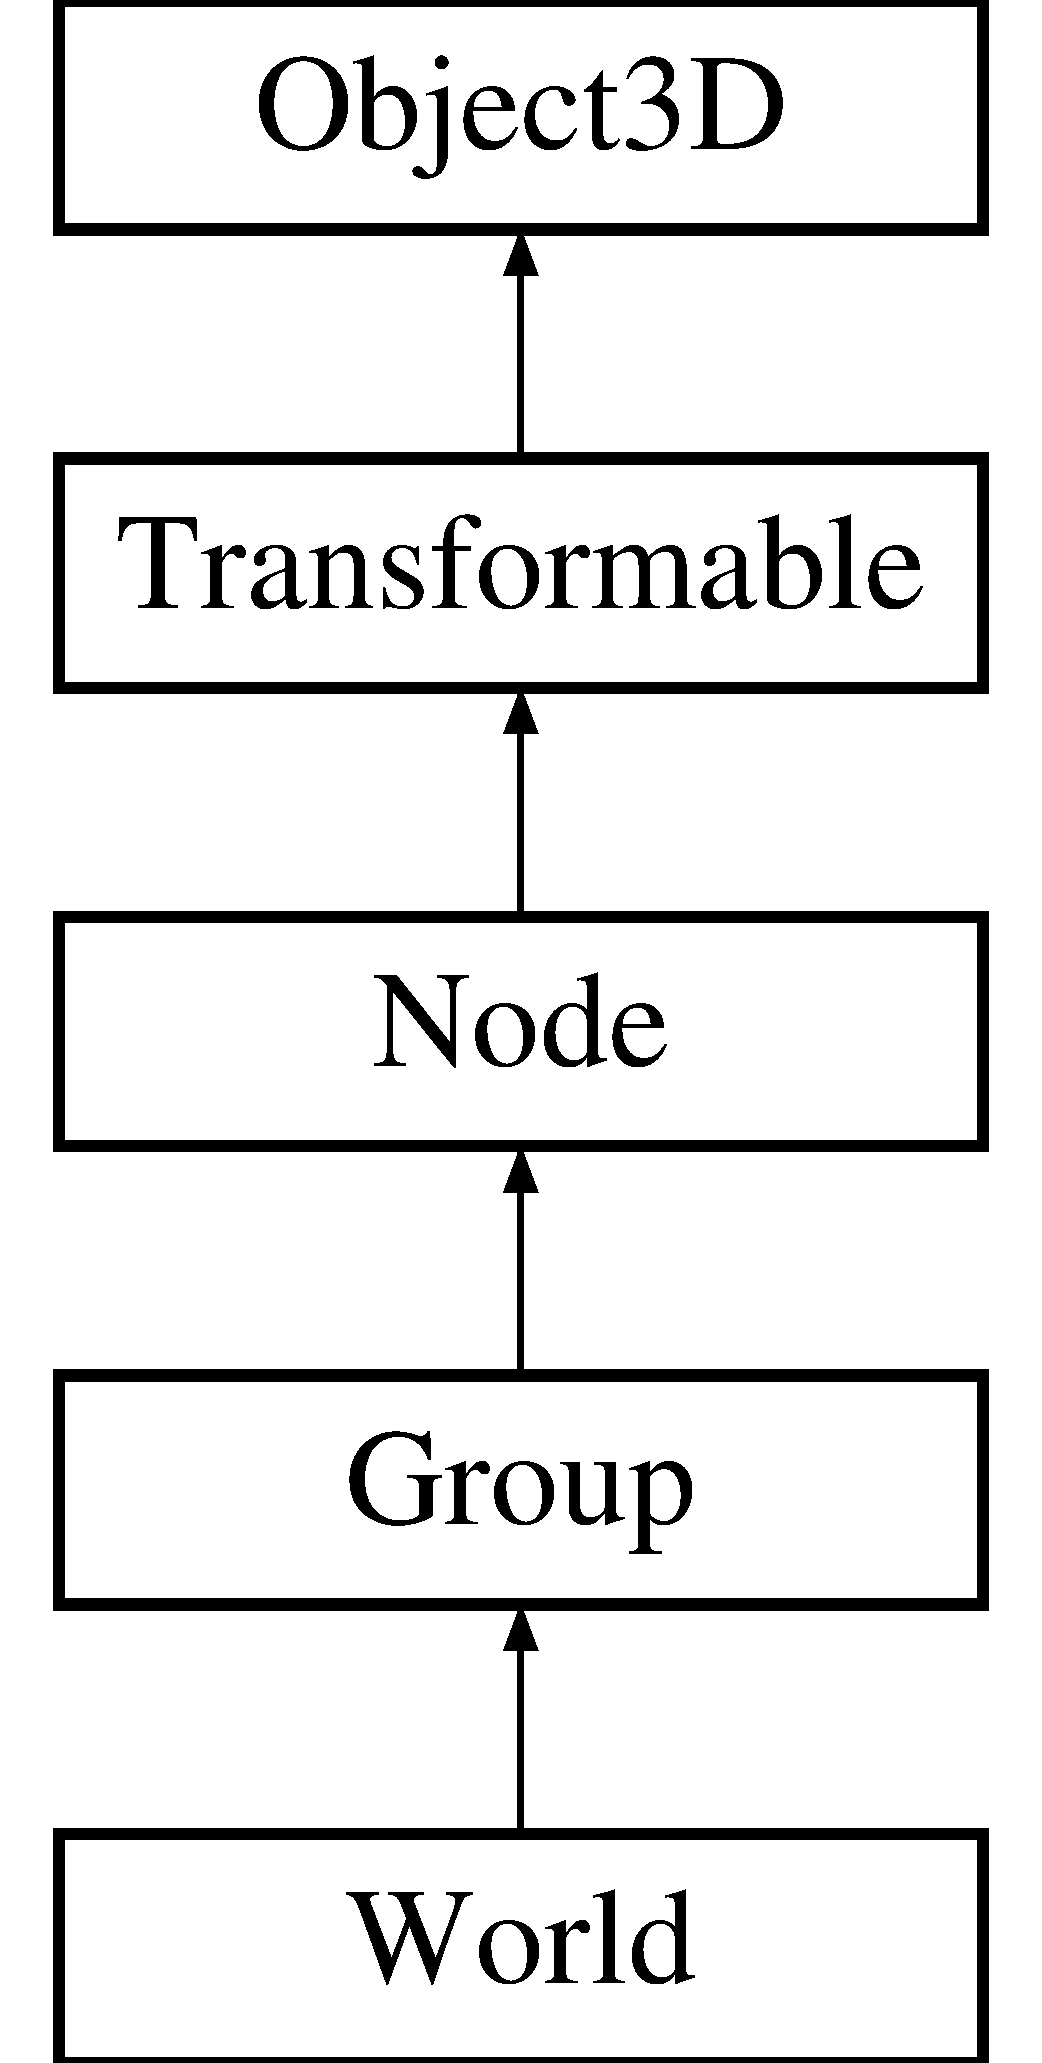
\includegraphics[height=6cm]{classm3g_1_1Group}
\end{center}
\end{figure}
\subsection*{Public メソッド}
\begin{CompactItemize}
\item 
\hyperlink{classm3g_1_1Group_0b29b9393b4b6856ac75b759f4166c13}{Group} ()
\item 
virtual \hyperlink{classm3g_1_1Group_a2a755272411c0d861f46f30970f5ca5}{$\sim$Group} ()
\item 
virtual \hyperlink{classm3g_1_1Group}{Group} $\ast$ \hyperlink{classm3g_1_1Group_1212dbd493e73180a6204874bd97df6b}{duplicate} () const 
\item 
void \hyperlink{classm3g_1_1Group_f7c798f6f7924dc14403df261f82153a}{addChild} (\hyperlink{classm3g_1_1Node}{Node} $\ast$child)
\item 
virtual int \hyperlink{classm3g_1_1Group_8aad1ceab4c2a03609c8a42324ce484d}{animate} (int world\_\-time)
\item 
\hyperlink{classm3g_1_1Node}{Node} $\ast$ \hyperlink{classm3g_1_1Group_a3af7d07fde341ef751157d274538698}{getChild} (int index) const 
\item 
int \hyperlink{classm3g_1_1Group_756d01dca16e146d69bb1881aca8fbb7}{getChildCount} () const 
\item 
bool \hyperlink{classm3g_1_1Group_10a3c77fa36fdb5d09b2bf39fe2a7c0b}{pick} (int scope, float ox, float oy, float oz, float dx, float dy, float dz, \hyperlink{classm3g_1_1RayIntersection}{RayIntersection} $\ast$ri) const 
\item 
void \hyperlink{classm3g_1_1Group_7415646c6f397f080d198176df44395c}{removeChild} (\hyperlink{classm3g_1_1Node}{Node} $\ast$child)
\item 
virtual std::ostream \& \hyperlink{classm3g_1_1Group_6fea17fa1532df3794f8cb39cb4f911f}{print} (std::ostream \&out) const 
\item 
virtual void \hyperlink{classm3g_1_1Group_8babc8a79b78615da51161e94029eea9}{render} (\hyperlink{structm3g_1_1RenderState}{RenderState} \&state) const 
\end{CompactItemize}
\subsection*{フレンド}
\begin{CompactItemize}
\item 
\hypertarget{classm3g_1_1Group_7b4bcdf992c21ae83363f25df05b1d25}{
class \textbf{World}}
\label{classm3g_1_1Group_7b4bcdf992c21ae83363f25df05b1d25}

\end{CompactItemize}


\subsection{説明}
未ソートの複数の子ノードを持つシーングラフのノード. 

\subsection{コンストラクタとデストラクタ}
\hypertarget{classm3g_1_1Group_0b29b9393b4b6856ac75b759f4166c13}{
\index{m3g::Group@{m3g::Group}!Group@{Group}}
\index{Group@{Group}!m3g::Group@{m3g::Group}}
\subsubsection[{Group}]{\setlength{\rightskip}{0pt plus 5cm}{\bf Group} ()}}
\label{classm3g_1_1Group_0b29b9393b4b6856ac75b759f4166c13}


子ノードを持たないGroupノードを作成するコンストラクタ. \hypertarget{classm3g_1_1Group_a2a755272411c0d861f46f30970f5ca5}{
\index{m3g::Group@{m3g::Group}!$\sim$Group@{$\sim$Group}}
\index{$\sim$Group@{$\sim$Group}!m3g::Group@{m3g::Group}}
\subsubsection[{$\sim$Group}]{\setlength{\rightskip}{0pt plus 5cm}$\sim${\bf Group} ()\hspace{0.3cm}{\tt  \mbox{[}virtual\mbox{]}}}}
\label{classm3g_1_1Group_a2a755272411c0d861f46f30970f5ca5}


デストラクタ. 

\subsection{関数}
\hypertarget{classm3g_1_1Group_f7c798f6f7924dc14403df261f82153a}{
\index{m3g::Group@{m3g::Group}!addChild@{addChild}}
\index{addChild@{addChild}!m3g::Group@{m3g::Group}}
\subsubsection[{addChild}]{\setlength{\rightskip}{0pt plus 5cm}void addChild ({\bf Node} $\ast$ {\em child})}}
\label{classm3g_1_1Group_f7c798f6f7924dc14403df261f82153a}


指定されたノードを追加する。以前に追加されていた子ノードの順番とインデックスは変更される可能性がある. \hypertarget{classm3g_1_1Group_8aad1ceab4c2a03609c8a42324ce484d}{
\index{m3g::Group@{m3g::Group}!animate@{animate}}
\index{animate@{animate}!m3g::Group@{m3g::Group}}
\subsubsection[{animate}]{\setlength{\rightskip}{0pt plus 5cm}int animate (int {\em world\_\-time})\hspace{0.3cm}{\tt  \mbox{[}virtual\mbox{]}}}}
\label{classm3g_1_1Group_8aad1ceab4c2a03609c8a42324ce484d}


このノードと子ノードをアニメーションする. 

\hyperlink{classm3g_1_1Node_8aad1ceab4c2a03609c8a42324ce484d}{Node}を再定義しています。

\hyperlink{classm3g_1_1World_8aad1ceab4c2a03609c8a42324ce484d}{World}で再定義されています。\hypertarget{classm3g_1_1Group_1212dbd493e73180a6204874bd97df6b}{
\index{m3g::Group@{m3g::Group}!duplicate@{duplicate}}
\index{duplicate@{duplicate}!m3g::Group@{m3g::Group}}
\subsubsection[{duplicate}]{\setlength{\rightskip}{0pt plus 5cm}{\bf Group} $\ast$ duplicate () const\hspace{0.3cm}{\tt  \mbox{[}virtual\mbox{]}}}}
\label{classm3g_1_1Group_1212dbd493e73180a6204874bd97df6b}


このオブジェクトの複製の作成. 

\hyperlink{classm3g_1_1Node_0b9f7531a4b56d34f47aeb1fff0d37e0}{Node}を再定義しています。

\hyperlink{classm3g_1_1World_efde97aaf753d48fff769d9011f187f2}{World}で再定義されています。\hypertarget{classm3g_1_1Group_a3af7d07fde341ef751157d274538698}{
\index{m3g::Group@{m3g::Group}!getChild@{getChild}}
\index{getChild@{getChild}!m3g::Group@{m3g::Group}}
\subsubsection[{getChild}]{\setlength{\rightskip}{0pt plus 5cm}{\bf Node} $\ast$ getChild (int {\em index}) const}}
\label{classm3g_1_1Group_a3af7d07fde341ef751157d274538698}


インデックスを指定して子ノードを取得する. \hypertarget{classm3g_1_1Group_756d01dca16e146d69bb1881aca8fbb7}{
\index{m3g::Group@{m3g::Group}!getChildCount@{getChildCount}}
\index{getChildCount@{getChildCount}!m3g::Group@{m3g::Group}}
\subsubsection[{getChildCount}]{\setlength{\rightskip}{0pt plus 5cm}int getChildCount () const}}
\label{classm3g_1_1Group_756d01dca16e146d69bb1881aca8fbb7}


このグループの子ノードの数を取得する. \hypertarget{classm3g_1_1Group_10a3c77fa36fdb5d09b2bf39fe2a7c0b}{
\index{m3g::Group@{m3g::Group}!pick@{pick}}
\index{pick@{pick}!m3g::Group@{m3g::Group}}
\subsubsection[{pick}]{\setlength{\rightskip}{0pt plus 5cm}bool pick (int {\em scope}, \/  float {\em ox}, \/  float {\em oy}, \/  float {\em oz}, \/  float {\em dx}, \/  float {\em dy}, \/  float {\em dz}, \/  {\bf RayIntersection} $\ast$ {\em ri}) const}}
\label{classm3g_1_1Group_10a3c77fa36fdb5d09b2bf39fe2a7c0b}


このグループのピッキング可能なMesh,scaled Sprite3Dのうち同じスコープで、指定されたピッキング光線で最初にヒットしたノードを返す. \hypertarget{classm3g_1_1Group_6fea17fa1532df3794f8cb39cb4f911f}{
\index{m3g::Group@{m3g::Group}!print@{print}}
\index{print@{print}!m3g::Group@{m3g::Group}}
\subsubsection[{print}]{\setlength{\rightskip}{0pt plus 5cm}std::ostream \& print (std::ostream \& {\em out}) const\hspace{0.3cm}{\tt  \mbox{[}virtual\mbox{]}}}}
\label{classm3g_1_1Group_6fea17fa1532df3794f8cb39cb4f911f}


このGroupクラスの情報を表示する。デバッグ用. 

\hyperlink{classm3g_1_1Node_6fea17fa1532df3794f8cb39cb4f911f}{Node}を再定義しています。

\hyperlink{classm3g_1_1World_6fea17fa1532df3794f8cb39cb4f911f}{World}で再定義されています。\hypertarget{classm3g_1_1Group_7415646c6f397f080d198176df44395c}{
\index{m3g::Group@{m3g::Group}!removeChild@{removeChild}}
\index{removeChild@{removeChild}!m3g::Group@{m3g::Group}}
\subsubsection[{removeChild}]{\setlength{\rightskip}{0pt plus 5cm}void removeChild ({\bf Node} $\ast$ {\em child})}}
\label{classm3g_1_1Group_7415646c6f397f080d198176df44395c}


このグループから指定されたノードを削除する。以前に追加されていた子ノードの順番とインデックスは変更される可能性がある. \hypertarget{classm3g_1_1Group_8babc8a79b78615da51161e94029eea9}{
\index{m3g::Group@{m3g::Group}!render@{render}}
\index{render@{render}!m3g::Group@{m3g::Group}}
\subsubsection[{render}]{\setlength{\rightskip}{0pt plus 5cm}void render ({\bf RenderState} \& {\em state}) const\hspace{0.3cm}{\tt  \mbox{[}virtual\mbox{]}}}}
\label{classm3g_1_1Group_8babc8a79b78615da51161e94029eea9}


このGroupをレンダリングする内部使用の関数.

Note: \hyperlink{classm3g_1_1Group}{Group} should be rendered via all rendering pass. 

\hyperlink{classm3g_1_1Node_8babc8a79b78615da51161e94029eea9}{Node}を再定義しています。

\hyperlink{classm3g_1_1World_8babc8a79b78615da51161e94029eea9}{World}で再定義されています。

このクラスの説明は次のファイルから生成されました:\begin{CompactItemize}
\item 
/work/workspace.desktop-m3g/src/Group.hpp\item 
/work/workspace.desktop-m3g/src/Group.cpp\end{CompactItemize}

\hypertarget{classm3g_1_1Image2D}{
\section{Image2D Class Reference}
\label{classm3g_1_1Image2D}\index{m3g::Image2D@{m3g::Image2D}}
}
{\tt \#include $<$Image2D.hpp$>$}

Inheritance diagram for Image2D::\begin{figure}[H]
\begin{center}
\leavevmode
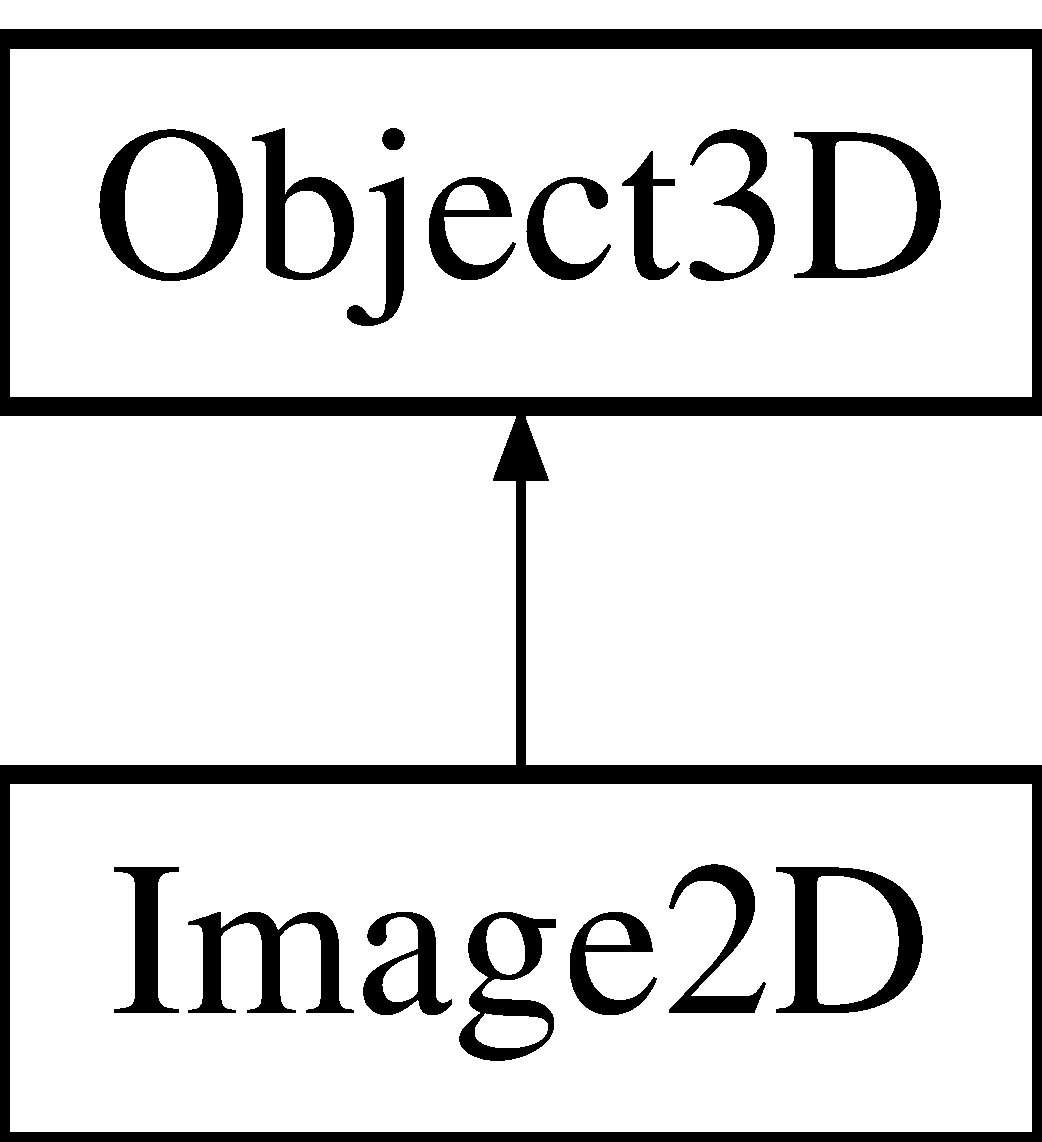
\includegraphics[height=3cm]{classm3g_1_1Image2D}
\end{center}
\end{figure}
\subsection*{Public Member Functions}
\begin{CompactItemize}
\item 
\hyperlink{classm3g_1_1Image2D_cea21be298c6584490d2b714c4b29d6b}{Image2D} (int format, int width, int height)
\item 
\hyperlink{classm3g_1_1Image2D_8cf9a47f24ed50fe66686c1117fb048c}{Image2D} (int format, int width, int height, void $\ast$image)
\item 
\hyperlink{classm3g_1_1Image2D_f498914ceac20ff9b1708c55ff1484e6}{Image2D} (int format, int width, int height, void $\ast$image, void $\ast$palette)
\item 
virtual \hyperlink{classm3g_1_1Image2D_7ac703fe7edbb053dd2246ea1bb43200}{$\sim$Image2D} ()
\item 
virtual \hyperlink{classm3g_1_1Image2D}{Image2D} $\ast$ \hyperlink{classm3g_1_1Image2D_47eefc8e0b0b3d4c5b16b3f57285fe6b}{duplicate} () const 
\item 
int \hyperlink{classm3g_1_1Image2D_c08e2752176d267cc4429d4d185975b8}{getFormat} () const 
\item 
int \hyperlink{classm3g_1_1Image2D_317329daf960a1759801c0f16d43d5a3}{getHeight} () const 
\item 
int \hyperlink{classm3g_1_1Image2D_f149cb053bc8b5fbc1364b5dbb934488}{getWidth} () const 
\item 
bool \hyperlink{classm3g_1_1Image2D_d687aabba553d1c66bfc253ec7e5bd05}{isMutable} () const 
\item 
void \hyperlink{classm3g_1_1Image2D_fe9ef1abefb9e92b38687e27c9004bdc}{set} (int x, int y, int width, int height, void $\ast$image)
\item 
void \hyperlink{classm3g_1_1Image2D_32ee5b2bcc9c7bf69b925413eeccb4bf}{write\_\-ppm} (const char $\ast$file\_\-name) const 
\item 
virtual std::ostream \& \hyperlink{classm3g_1_1Image2D_6fea17fa1532df3794f8cb39cb4f911f}{print} (std::ostream \&out) const 
\item 
GLenum \hyperlink{classm3g_1_1Image2D_7923da2fe82fee768ec9937a693e843c}{getOpenGLFormat} () const 
\item 
void $\ast$ \hyperlink{classm3g_1_1Image2D_b837b1bdda59947a6d818c448965c502}{getOpenGLData} () const 
\end{CompactItemize}
\subsection*{Static Public Attributes}
\begin{CompactItemize}
\item 
static const int \hyperlink{classm3g_1_1Image2D_417581fcde4067111f47320edb2aa378}{ALPHA} = 96
\item 
static const int \hyperlink{classm3g_1_1Image2D_3cf02f5117269e8ff112cbf5ecb790cd}{LUMINANCE} = 97
\item 
static const int \hyperlink{classm3g_1_1Image2D_1a74b878039f244c27120cacb4eb6a3e}{LUMINANCE\_\-ALPHA} = 98
\item 
static const int \hyperlink{classm3g_1_1Image2D_5f237f1b0f2ce6351e9e4a494b8dc759}{RGB} = 99
\item 
static const int \hyperlink{classm3g_1_1Image2D_0aaf9f2f4c064633c6d2888ec2c39e92}{RGBA} = 100
\end{CompactItemize}
\subsection*{Friends}
\begin{CompactItemize}
\item 
\hypertarget{classm3g_1_1Image2D_a70951a0328ba29f64176f16b3ea47d8}{
class \textbf{Texture2D}}
\label{classm3g_1_1Image2D_a70951a0328ba29f64176f16b3ea47d8}

\item 
\hypertarget{classm3g_1_1Image2D_d70dac188b152e81b4323bb274bee959}{
class \textbf{Background}}
\label{classm3g_1_1Image2D_d70dac188b152e81b4323bb274bee959}

\item 
\hypertarget{classm3g_1_1Image2D_639cf38c41878a4f0fc8d24c010c96de}{
class \textbf{Sprite3D}}
\label{classm3g_1_1Image2D_639cf38c41878a4f0fc8d24c010c96de}

\end{CompactItemize}


\subsection{Detailed Description}
A two-dimensional image that can be used as a textur, backgoround or sprite image. 

\subsection{Constructor \& Destructor Documentation}
\hypertarget{classm3g_1_1Image2D_cea21be298c6584490d2b714c4b29d6b}{
\index{m3g::Image2D@{m3g::Image2D}!Image2D@{Image2D}}
\index{Image2D@{Image2D}!m3g::Image2D@{m3g::Image2D}}
\subsubsection[{Image2D}]{\setlength{\rightskip}{0pt plus 5cm}{\bf Image2D} (int {\em format}, \/  int {\em width}, \/  int {\em height})}}
\label{classm3g_1_1Image2D_cea21be298c6584490d2b714c4b29d6b}


Construct an empty, mutable \hyperlink{classm3g_1_1Image2D}{Image2D} with the given dimensions. \hypertarget{classm3g_1_1Image2D_8cf9a47f24ed50fe66686c1117fb048c}{
\index{m3g::Image2D@{m3g::Image2D}!Image2D@{Image2D}}
\index{Image2D@{Image2D}!m3g::Image2D@{m3g::Image2D}}
\subsubsection[{Image2D}]{\setlength{\rightskip}{0pt plus 5cm}{\bf Image2D} (int {\em format}, \/  int {\em width}, \/  int {\em height}, \/  void $\ast$ {\em image})}}
\label{classm3g_1_1Image2D_8cf9a47f24ed50fe66686c1117fb048c}


Costrucsts an immutable \hyperlink{classm3g_1_1Image2D}{Image2D} by copying pixels from a byte array. \hypertarget{classm3g_1_1Image2D_f498914ceac20ff9b1708c55ff1484e6}{
\index{m3g::Image2D@{m3g::Image2D}!Image2D@{Image2D}}
\index{Image2D@{Image2D}!m3g::Image2D@{m3g::Image2D}}
\subsubsection[{Image2D}]{\setlength{\rightskip}{0pt plus 5cm}{\bf Image2D} (int {\em format}, \/  int {\em width}, \/  int {\em height}, \/  void $\ast$ {\em image}, \/  void $\ast$ {\em palette})}}
\label{classm3g_1_1Image2D_f498914ceac20ff9b1708c55ff1484e6}


Constructs an immutable \hyperlink{classm3g_1_1Image2D}{Image2D} by copying palette indices from a byte array, and the palette enttries from another byte array. \hypertarget{classm3g_1_1Image2D_7ac703fe7edbb053dd2246ea1bb43200}{
\index{m3g::Image2D@{m3g::Image2D}!$\sim$Image2D@{$\sim$Image2D}}
\index{$\sim$Image2D@{$\sim$Image2D}!m3g::Image2D@{m3g::Image2D}}
\subsubsection[{$\sim$Image2D}]{\setlength{\rightskip}{0pt plus 5cm}$\sim${\bf Image2D} ()\hspace{0.3cm}{\tt  \mbox{[}virtual\mbox{]}}}}
\label{classm3g_1_1Image2D_7ac703fe7edbb053dd2246ea1bb43200}


Destruct this object. 

\subsection{Member Function Documentation}
\hypertarget{classm3g_1_1Image2D_47eefc8e0b0b3d4c5b16b3f57285fe6b}{
\index{m3g::Image2D@{m3g::Image2D}!duplicate@{duplicate}}
\index{duplicate@{duplicate}!m3g::Image2D@{m3g::Image2D}}
\subsubsection[{duplicate}]{\setlength{\rightskip}{0pt plus 5cm}{\bf Image2D} $\ast$ duplicate () const\hspace{0.3cm}{\tt  \mbox{[}virtual\mbox{]}}}}
\label{classm3g_1_1Image2D_47eefc8e0b0b3d4c5b16b3f57285fe6b}


Creates a duplicate of this \hyperlink{classm3g_1_1Object3D}{Object3D}. 

Reimplemented from \hyperlink{classm3g_1_1Object3D_a25110dac934f867b83b73ad4741a0f4}{Object3D}.\hypertarget{classm3g_1_1Image2D_c08e2752176d267cc4429d4d185975b8}{
\index{m3g::Image2D@{m3g::Image2D}!getFormat@{getFormat}}
\index{getFormat@{getFormat}!m3g::Image2D@{m3g::Image2D}}
\subsubsection[{getFormat}]{\setlength{\rightskip}{0pt plus 5cm}int getFormat () const}}
\label{classm3g_1_1Image2D_c08e2752176d267cc4429d4d185975b8}


Gets the internal format of this \hyperlink{classm3g_1_1Image2D}{Image2D}. \hypertarget{classm3g_1_1Image2D_317329daf960a1759801c0f16d43d5a3}{
\index{m3g::Image2D@{m3g::Image2D}!getHeight@{getHeight}}
\index{getHeight@{getHeight}!m3g::Image2D@{m3g::Image2D}}
\subsubsection[{getHeight}]{\setlength{\rightskip}{0pt plus 5cm}int getHeight () const}}
\label{classm3g_1_1Image2D_317329daf960a1759801c0f16d43d5a3}


Gets the hieght of this \hyperlink{classm3g_1_1Image2D}{Image2D}. \hypertarget{classm3g_1_1Image2D_b837b1bdda59947a6d818c448965c502}{
\index{m3g::Image2D@{m3g::Image2D}!getOpenGLData@{getOpenGLData}}
\index{getOpenGLData@{getOpenGLData}!m3g::Image2D@{m3g::Image2D}}
\subsubsection[{getOpenGLData}]{\setlength{\rightskip}{0pt plus 5cm}void $\ast$ getOpenGLData () const}}
\label{classm3g_1_1Image2D_b837b1bdda59947a6d818c448965c502}


Return pointer to raw data, for inner use. \hypertarget{classm3g_1_1Image2D_7923da2fe82fee768ec9937a693e843c}{
\index{m3g::Image2D@{m3g::Image2D}!getOpenGLFormat@{getOpenGLFormat}}
\index{getOpenGLFormat@{getOpenGLFormat}!m3g::Image2D@{m3g::Image2D}}
\subsubsection[{getOpenGLFormat}]{\setlength{\rightskip}{0pt plus 5cm}GLenum getOpenGLFormat () const}}
\label{classm3g_1_1Image2D_7923da2fe82fee768ec9937a693e843c}


Return OpenGL format, for inner use. \hypertarget{classm3g_1_1Image2D_f149cb053bc8b5fbc1364b5dbb934488}{
\index{m3g::Image2D@{m3g::Image2D}!getWidth@{getWidth}}
\index{getWidth@{getWidth}!m3g::Image2D@{m3g::Image2D}}
\subsubsection[{getWidth}]{\setlength{\rightskip}{0pt plus 5cm}int getWidth () const}}
\label{classm3g_1_1Image2D_f149cb053bc8b5fbc1364b5dbb934488}


Gets the width of this \hyperlink{classm3g_1_1Image2D}{Image2D}. \hypertarget{classm3g_1_1Image2D_d687aabba553d1c66bfc253ec7e5bd05}{
\index{m3g::Image2D@{m3g::Image2D}!isMutable@{isMutable}}
\index{isMutable@{isMutable}!m3g::Image2D@{m3g::Image2D}}
\subsubsection[{isMutable}]{\setlength{\rightskip}{0pt plus 5cm}bool isMutable () const}}
\label{classm3g_1_1Image2D_d687aabba553d1c66bfc253ec7e5bd05}


Qeries wheter this \hyperlink{classm3g_1_1Image2D}{Image2D} is mutable. \hypertarget{classm3g_1_1Image2D_6fea17fa1532df3794f8cb39cb4f911f}{
\index{m3g::Image2D@{m3g::Image2D}!print@{print}}
\index{print@{print}!m3g::Image2D@{m3g::Image2D}}
\subsubsection[{print}]{\setlength{\rightskip}{0pt plus 5cm}std::ostream \& print (std::ostream \& {\em out}) const\hspace{0.3cm}{\tt  \mbox{[}virtual\mbox{]}}}}
\label{classm3g_1_1Image2D_6fea17fa1532df3794f8cb39cb4f911f}


Print out information of this class, for only debug. 

Reimplemented from \hyperlink{classm3g_1_1Object3D_6fea17fa1532df3794f8cb39cb4f911f}{Object3D}.\hypertarget{classm3g_1_1Image2D_fe9ef1abefb9e92b38687e27c9004bdc}{
\index{m3g::Image2D@{m3g::Image2D}!set@{set}}
\index{set@{set}!m3g::Image2D@{m3g::Image2D}}
\subsubsection[{set}]{\setlength{\rightskip}{0pt plus 5cm}void set (int {\em x}, \/  int {\em y}, \/  int {\em width}, \/  int {\em height}, \/  void $\ast$ {\em image})}}
\label{classm3g_1_1Image2D_fe9ef1abefb9e92b38687e27c9004bdc}


Updates a rectangular area of this \hyperlink{classm3g_1_1Image2D}{Image2D} by copying pixels from a byte array. \hypertarget{classm3g_1_1Image2D_32ee5b2bcc9c7bf69b925413eeccb4bf}{
\index{m3g::Image2D@{m3g::Image2D}!write\_\-ppm@{write\_\-ppm}}
\index{write\_\-ppm@{write\_\-ppm}!m3g::Image2D@{m3g::Image2D}}
\subsubsection[{write\_\-ppm}]{\setlength{\rightskip}{0pt plus 5cm}void write\_\-ppm (const char $\ast$ {\em name}) const}}
\label{classm3g_1_1Image2D_32ee5b2bcc9c7bf69b925413eeccb4bf}


Write image as ppm file(alpha component is ignored), for only debug .

注意:OpenGLは左下が(0,0)、ppmは左上が(0,0) 

\subsection{Member Data Documentation}
\hypertarget{classm3g_1_1Image2D_417581fcde4067111f47320edb2aa378}{
\index{m3g::Image2D@{m3g::Image2D}!ALPHA@{ALPHA}}
\index{ALPHA@{ALPHA}!m3g::Image2D@{m3g::Image2D}}
\subsubsection[{ALPHA}]{\setlength{\rightskip}{0pt plus 5cm}const int {\bf ALPHA} = 96\hspace{0.3cm}{\tt  \mbox{[}static\mbox{]}}}}
\label{classm3g_1_1Image2D_417581fcde4067111f47320edb2aa378}


A constructor parameter specifying that this \hyperlink{classm3g_1_1Image2D}{Image2D} has an alpha component only. \hypertarget{classm3g_1_1Image2D_3cf02f5117269e8ff112cbf5ecb790cd}{
\index{m3g::Image2D@{m3g::Image2D}!LUMINANCE@{LUMINANCE}}
\index{LUMINANCE@{LUMINANCE}!m3g::Image2D@{m3g::Image2D}}
\subsubsection[{LUMINANCE}]{\setlength{\rightskip}{0pt plus 5cm}const int {\bf LUMINANCE} = 97\hspace{0.3cm}{\tt  \mbox{[}static\mbox{]}}}}
\label{classm3g_1_1Image2D_3cf02f5117269e8ff112cbf5ecb790cd}


A constructor parameter specifying that this \hyperlink{classm3g_1_1Image2D}{Image2D} has a luminance component only. \hypertarget{classm3g_1_1Image2D_1a74b878039f244c27120cacb4eb6a3e}{
\index{m3g::Image2D@{m3g::Image2D}!LUMINANCE\_\-ALPHA@{LUMINANCE\_\-ALPHA}}
\index{LUMINANCE\_\-ALPHA@{LUMINANCE\_\-ALPHA}!m3g::Image2D@{m3g::Image2D}}
\subsubsection[{LUMINANCE\_\-ALPHA}]{\setlength{\rightskip}{0pt plus 5cm}const int {\bf LUMINANCE\_\-ALPHA} = 98\hspace{0.3cm}{\tt  \mbox{[}static\mbox{]}}}}
\label{classm3g_1_1Image2D_1a74b878039f244c27120cacb4eb6a3e}


A constructor parameter specifying that this \hyperlink{classm3g_1_1Image2D}{Image2D} has luminance and an alpha component only. \hypertarget{classm3g_1_1Image2D_5f237f1b0f2ce6351e9e4a494b8dc759}{
\index{m3g::Image2D@{m3g::Image2D}!RGB@{RGB}}
\index{RGB@{RGB}!m3g::Image2D@{m3g::Image2D}}
\subsubsection[{RGB}]{\setlength{\rightskip}{0pt plus 5cm}const int {\bf RGB} = 99\hspace{0.3cm}{\tt  \mbox{[}static\mbox{]}}}}
\label{classm3g_1_1Image2D_5f237f1b0f2ce6351e9e4a494b8dc759}


A constructor parameter specifying that this \hyperlink{classm3g_1_1Image2D}{Image2D} has red, green and blue color components. \hypertarget{classm3g_1_1Image2D_0aaf9f2f4c064633c6d2888ec2c39e92}{
\index{m3g::Image2D@{m3g::Image2D}!RGBA@{RGBA}}
\index{RGBA@{RGBA}!m3g::Image2D@{m3g::Image2D}}
\subsubsection[{RGBA}]{\setlength{\rightskip}{0pt plus 5cm}const int {\bf RGBA} = 100\hspace{0.3cm}{\tt  \mbox{[}static\mbox{]}}}}
\label{classm3g_1_1Image2D_0aaf9f2f4c064633c6d2888ec2c39e92}


A constructor parameter specifying that this \hyperlink{classm3g_1_1Image2D}{Image2D} has red, green, blue and alpha color components. 

The documentation for this class was generated from the following files:\begin{CompactItemize}
\item 
/work/workspace.desktop-m3g/src/Image2D.hpp\item 
/work/workspace.desktop-m3g/src/Image2D.cpp\end{CompactItemize}

\hypertarget{classm3g_1_1IndexBuffer}{
\section{クラス IndexBuffer}
\label{classm3g_1_1IndexBuffer}\index{m3g::IndexBuffer@{m3g::IndexBuffer}}
}
{\tt \#include $<$IndexBuffer.hpp$>$}

IndexBufferに対する継承グラフ:\begin{figure}[H]
\begin{center}
\leavevmode
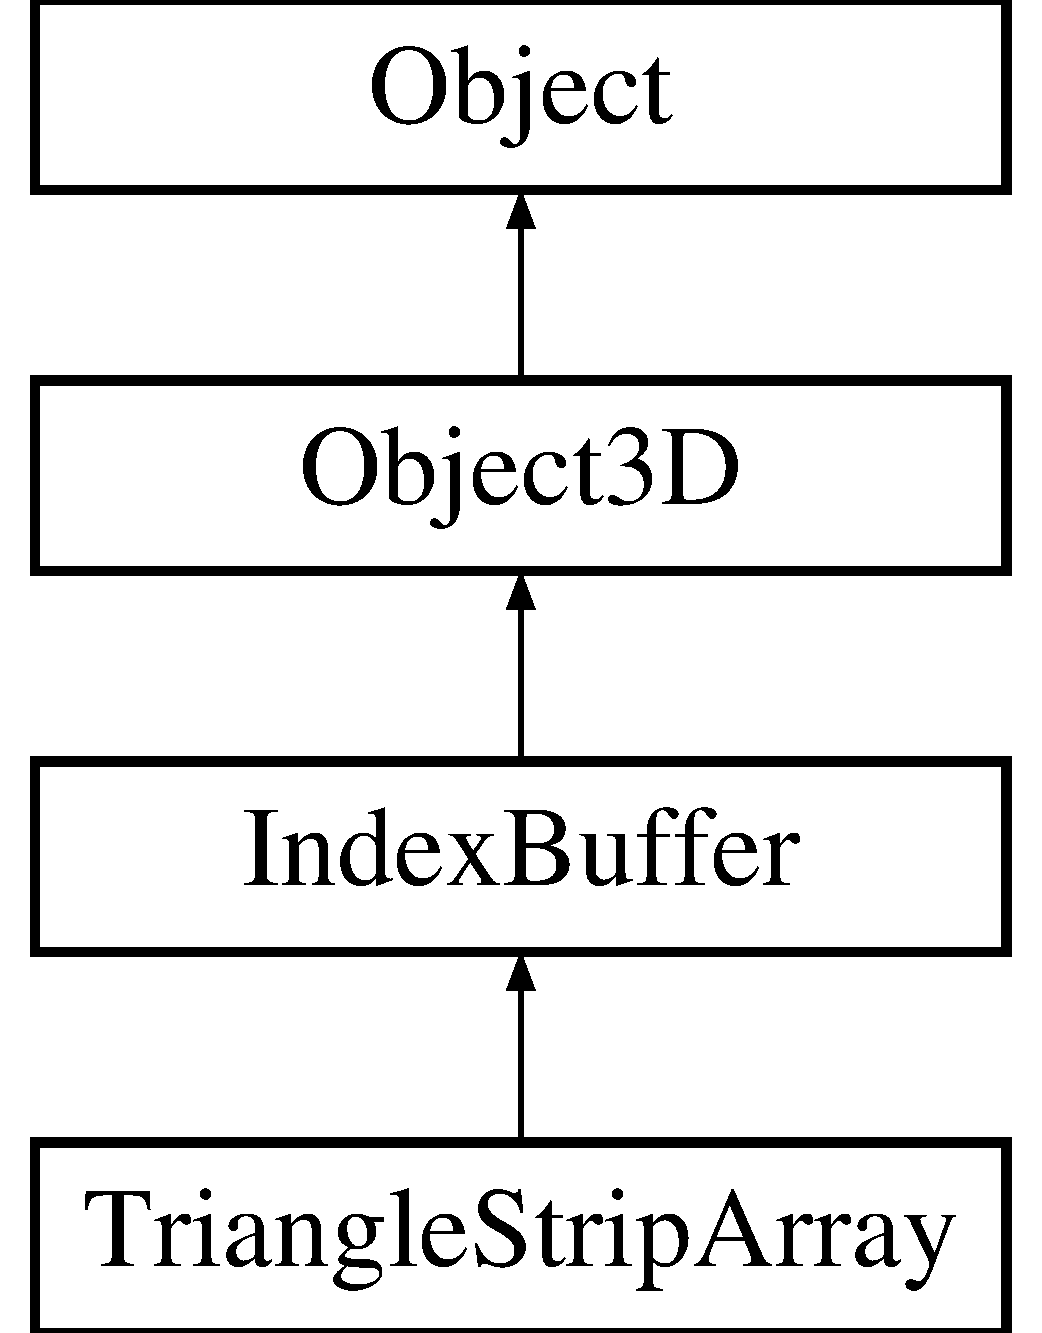
\includegraphics[height=4cm]{classm3g_1_1IndexBuffer}
\end{center}
\end{figure}
\subsection*{Public メソッド}
\begin{CompactItemize}
\item 
\hyperlink{classm3g_1_1IndexBuffer_d2e68a2d7c6c753d3abfeef42ee79427}{IndexBuffer} ()
\item 
virtual \hyperlink{classm3g_1_1IndexBuffer_ac7952364fe4d2d7b2731da5380c841c}{$\sim$IndexBuffer} ()
\item 
virtual \hyperlink{classm3g_1_1IndexBuffer}{IndexBuffer} $\ast$ \hyperlink{classm3g_1_1IndexBuffer_fab6fc0a0ec393e527f849c3af10ad76}{duplicate} () const 
\item 
virtual int \hyperlink{classm3g_1_1IndexBuffer_fe9ae2993ebcdb93d5ff26d57c81b73e}{getIndexCount} () const 
\item 
virtual void \hyperlink{classm3g_1_1IndexBuffer_650953afac45099025a524ab160b911f}{getIndices} (int $\ast$indices)
\item 
virtual std::ostream \& \hyperlink{classm3g_1_1IndexBuffer_6fea17fa1532df3794f8cb39cb4f911f}{print} (std::ostream \&out) const 
\end{CompactItemize}
\subsection*{Protected メソッド}
\begin{CompactItemize}
\item 
virtual void \hyperlink{classm3g_1_1IndexBuffer_8babc8a79b78615da51161e94029eea9}{render} (\hyperlink{structm3g_1_1RenderState}{RenderState} \&state) const 
\end{CompactItemize}
\subsection*{フレンド}
\begin{CompactItemize}
\item 
\hypertarget{classm3g_1_1IndexBuffer_a41a130f156b145bffb3f4b5172c4c93}{
class \textbf{Mesh}}
\label{classm3g_1_1IndexBuffer_a41a130f156b145bffb3f4b5172c4c93}

\end{CompactItemize}


\subsection{説明}
頂点を連結し幾何形状を定義する抽象クラス. 

\subsection{コンストラクタとデストラクタ}
\hypertarget{classm3g_1_1IndexBuffer_d2e68a2d7c6c753d3abfeef42ee79427}{
\index{m3g::IndexBuffer@{m3g::IndexBuffer}!IndexBuffer@{IndexBuffer}}
\index{IndexBuffer@{IndexBuffer}!m3g::IndexBuffer@{m3g::IndexBuffer}}
\subsubsection[{IndexBuffer}]{\setlength{\rightskip}{0pt plus 5cm}{\bf IndexBuffer} ()}}
\label{classm3g_1_1IndexBuffer_d2e68a2d7c6c753d3abfeef42ee79427}


新しいIndexBufferオブジェクトを作成するコンストラクタ. \hypertarget{classm3g_1_1IndexBuffer_ac7952364fe4d2d7b2731da5380c841c}{
\index{m3g::IndexBuffer@{m3g::IndexBuffer}!$\sim$IndexBuffer@{$\sim$IndexBuffer}}
\index{$\sim$IndexBuffer@{$\sim$IndexBuffer}!m3g::IndexBuffer@{m3g::IndexBuffer}}
\subsubsection[{$\sim$IndexBuffer}]{\setlength{\rightskip}{0pt plus 5cm}$\sim${\bf IndexBuffer} ()\hspace{0.3cm}{\tt  \mbox{[}virtual\mbox{]}}}}
\label{classm3g_1_1IndexBuffer_ac7952364fe4d2d7b2731da5380c841c}


デストラクタ. 

\subsection{関数}
\hypertarget{classm3g_1_1IndexBuffer_fab6fc0a0ec393e527f849c3af10ad76}{
\index{m3g::IndexBuffer@{m3g::IndexBuffer}!duplicate@{duplicate}}
\index{duplicate@{duplicate}!m3g::IndexBuffer@{m3g::IndexBuffer}}
\subsubsection[{duplicate}]{\setlength{\rightskip}{0pt plus 5cm}{\bf IndexBuffer} $\ast$ duplicate () const\hspace{0.3cm}{\tt  \mbox{[}virtual\mbox{]}}}}
\label{classm3g_1_1IndexBuffer_fab6fc0a0ec393e527f849c3af10ad76}


このオブジェクトの複製の作成. 

\hyperlink{classm3g_1_1Object3D_a25110dac934f867b83b73ad4741a0f4}{Object3D}を再定義しています。

\hyperlink{classm3g_1_1TriangleStripArray_1623fbdfe91eb2e9d4a67bece6a46904}{TriangleStripArray}で再定義されています。\hypertarget{classm3g_1_1IndexBuffer_fe9ae2993ebcdb93d5ff26d57c81b73e}{
\index{m3g::IndexBuffer@{m3g::IndexBuffer}!getIndexCount@{getIndexCount}}
\index{getIndexCount@{getIndexCount}!m3g::IndexBuffer@{m3g::IndexBuffer}}
\subsubsection[{getIndexCount}]{\setlength{\rightskip}{0pt plus 5cm}int getIndexCount () const\hspace{0.3cm}{\tt  \mbox{[}virtual\mbox{]}}}}
\label{classm3g_1_1IndexBuffer_fe9ae2993ebcdb93d5ff26d57c81b73e}


このバッファーのインデックスの数を取得. 

\hyperlink{classm3g_1_1TriangleStripArray_fe9ae2993ebcdb93d5ff26d57c81b73e}{TriangleStripArray}で再定義されています。\hypertarget{classm3g_1_1IndexBuffer_650953afac45099025a524ab160b911f}{
\index{m3g::IndexBuffer@{m3g::IndexBuffer}!getIndices@{getIndices}}
\index{getIndices@{getIndices}!m3g::IndexBuffer@{m3g::IndexBuffer}}
\subsubsection[{getIndices}]{\setlength{\rightskip}{0pt plus 5cm}void getIndices (int $\ast$ {\em indices})\hspace{0.3cm}{\tt  \mbox{[}virtual\mbox{]}}}}
\label{classm3g_1_1IndexBuffer_650953afac45099025a524ab160b911f}


このバッファーに収納されているインデックスを取得. 

\hyperlink{classm3g_1_1TriangleStripArray_650953afac45099025a524ab160b911f}{TriangleStripArray}で再定義されています。\hypertarget{classm3g_1_1IndexBuffer_6fea17fa1532df3794f8cb39cb4f911f}{
\index{m3g::IndexBuffer@{m3g::IndexBuffer}!print@{print}}
\index{print@{print}!m3g::IndexBuffer@{m3g::IndexBuffer}}
\subsubsection[{print}]{\setlength{\rightskip}{0pt plus 5cm}std::ostream \& print (std::ostream \& {\em out}) const\hspace{0.3cm}{\tt  \mbox{[}virtual\mbox{]}}}}
\label{classm3g_1_1IndexBuffer_6fea17fa1532df3794f8cb39cb4f911f}


このImage2Dクラスの情報を表示する。デバッグ用. 

\hyperlink{classm3g_1_1Object3D_6fea17fa1532df3794f8cb39cb4f911f}{Object3D}を再定義しています。

\hyperlink{classm3g_1_1TriangleStripArray_6fea17fa1532df3794f8cb39cb4f911f}{TriangleStripArray}で再定義されています。\hypertarget{classm3g_1_1IndexBuffer_8babc8a79b78615da51161e94029eea9}{
\index{m3g::IndexBuffer@{m3g::IndexBuffer}!render@{render}}
\index{render@{render}!m3g::IndexBuffer@{m3g::IndexBuffer}}
\subsubsection[{render}]{\setlength{\rightskip}{0pt plus 5cm}void render ({\bf RenderState} \& {\em state}) const\hspace{0.3cm}{\tt  \mbox{[}protected, virtual\mbox{]}}}}
\label{classm3g_1_1IndexBuffer_8babc8a79b78615da51161e94029eea9}


このIndexBufferをレンダリングする内部使用の関数.

Note: \hyperlink{classm3g_1_1Background}{Background} should be rendered only at second rendering pass(pass=2). In other cases, do nothing. 

\hyperlink{classm3g_1_1Object3D_8babc8a79b78615da51161e94029eea9}{Object3D}を再定義しています。

\hyperlink{classm3g_1_1TriangleStripArray_8babc8a79b78615da51161e94029eea9}{TriangleStripArray}で再定義されています。

このクラスの説明は次のファイルから生成されました:\begin{CompactItemize}
\item 
/work/workspace.desktop-m3g/src/IndexBuffer.hpp\item 
/work/workspace.desktop-m3g/src/IndexBuffer.cpp\end{CompactItemize}

\hypertarget{classm3g_1_1Keyframe}{
\section{クラス Keyframe}
\label{classm3g_1_1Keyframe}\index{m3g::Keyframe@{m3g::Keyframe}}
}
{\tt \#include $<$Keyframe.hpp$>$}

\subsection*{Public メソッド}
\begin{CompactItemize}
\item 
\hypertarget{classm3g_1_1Keyframe_8d7b239b0b22e155001b100c80a9680b}{
\textbf{Keyframe} (int t, float $\ast$v)}
\label{classm3g_1_1Keyframe_8d7b239b0b22e155001b100c80a9680b}

\item 
std::ostream \& \hyperlink{classm3g_1_1Keyframe_6fea17fa1532df3794f8cb39cb4f911f}{print} (std::ostream \&out) const 
\end{CompactItemize}
\subsection*{Public 変数}
\begin{CompactItemize}
\item 
\hypertarget{classm3g_1_1Keyframe_42715f65f02da52edc5b22021d8ae670}{
int \textbf{time}}
\label{classm3g_1_1Keyframe_42715f65f02da52edc5b22021d8ae670}

\item 
\hypertarget{classm3g_1_1Keyframe_b8d14ba2f5911cadc861b9b89ae0c605}{
float $\ast$ \textbf{value}}
\label{classm3g_1_1Keyframe_b8d14ba2f5911cadc861b9b89ae0c605}

\end{CompactItemize}


\subsection{説明}
キーフレーム情報を定義する内部使用構造体. time=-1は無効データを表す。 

\subsection{関数}
\hypertarget{classm3g_1_1Keyframe_6fea17fa1532df3794f8cb39cb4f911f}{
\index{m3g::Keyframe@{m3g::Keyframe}!print@{print}}
\index{print@{print}!m3g::Keyframe@{m3g::Keyframe}}
\subsubsection[{print}]{\setlength{\rightskip}{0pt plus 5cm}std::ostream \& print (std::ostream \& {\em out}) const}}
\label{classm3g_1_1Keyframe_6fea17fa1532df3794f8cb39cb4f911f}


このオブジェクトの情報を表示する内部使用の関数, デバッグ用. 

このクラスの説明は次のファイルから生成されました:\begin{CompactItemize}
\item 
/work/workspace.desktop-m3g/src/Keyframe.hpp\item 
/work/workspace.desktop-m3g/src/Keyframe.cpp\end{CompactItemize}

\hypertarget{classm3g_1_1KeyframeSequence}{
\section{KeyframeSequence Class Reference}
\label{classm3g_1_1KeyframeSequence}\index{m3g::KeyframeSequence@{m3g::KeyframeSequence}}
}
{\tt \#include $<$KeyframeSequence.hpp$>$}

Inheritance diagram for KeyframeSequence::\begin{figure}[H]
\begin{center}
\leavevmode
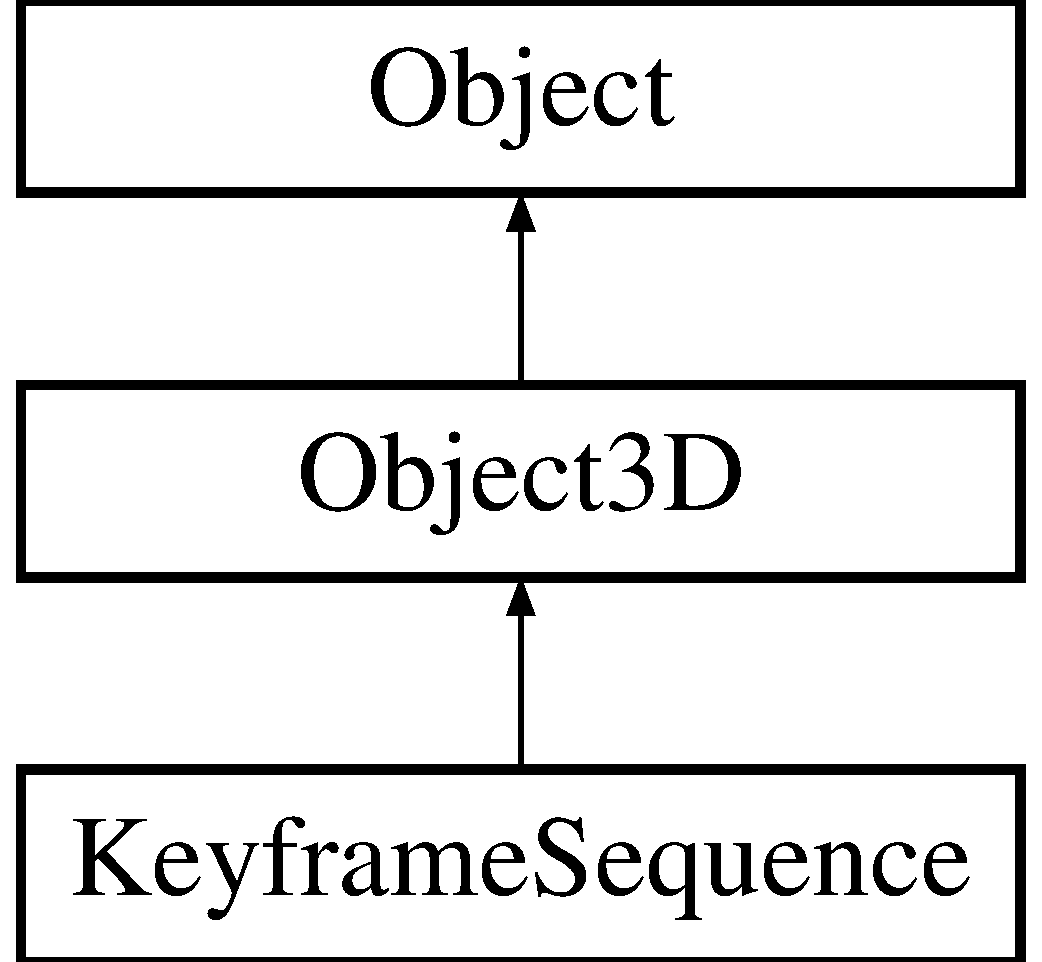
\includegraphics[height=3cm]{classm3g_1_1KeyframeSequence}
\end{center}
\end{figure}
\subsection*{Classes}
\begin{CompactItemize}
\item 
struct \hyperlink{structm3g_1_1KeyframeSequence_1_1ValidRange}{ValidRange}
\end{CompactItemize}
\subsection*{Public Member Functions}
\begin{CompactItemize}
\item 
\hyperlink{classm3g_1_1KeyframeSequence_f48cc8113ad7300d72840b18529aaf0e}{KeyframeSequence} (int num\_\-keyframes, int num\_\-components, int interpolation)
\item 
virtual \hyperlink{classm3g_1_1KeyframeSequence_464f5929e3302c788ca626c11ca8d656}{$\sim$KeyframeSequence} ()
\item 
virtual \hyperlink{classm3g_1_1KeyframeSequence}{KeyframeSequence} $\ast$ \hyperlink{classm3g_1_1KeyframeSequence_f925b7c3107b6cdba08dbb045b203b4f}{duplicate} () const 
\item 
int \hyperlink{classm3g_1_1KeyframeSequence_7016f51d2788e78fdd736efd040f5e5e}{getComponentCount} () const 
\item 
int \hyperlink{classm3g_1_1KeyframeSequence_995a5ca5c8c3c993ef167f67cbb5fabe}{getDuration} () const 
\item 
int \hyperlink{classm3g_1_1KeyframeSequence_0d46321e7f46e037508cce88cdf6a487}{getInterpolationType} () const 
\item 
int \hyperlink{classm3g_1_1KeyframeSequence_0fd27047149eedab8b10319768e1fe9a}{getKeyframe} (int index, float $\ast$value) const 
\item 
int \hyperlink{classm3g_1_1KeyframeSequence_4d500a603f25adafd8e6f8b68872dbff}{getKeyframeCount} () const 
\item 
int \hyperlink{classm3g_1_1KeyframeSequence_a356af60b9759d5d3da833773e3c7b73}{getRepeatMode} () const 
\item 
int \hyperlink{classm3g_1_1KeyframeSequence_b7e54386674cefdb8f5fa65ce5435b50}{getValidRangeFirst} () const 
\item 
int \hyperlink{classm3g_1_1KeyframeSequence_aa98cc8d698c482c33a3487c33db27d0}{getValidRangeLast} () const 
\item 
void \hyperlink{classm3g_1_1KeyframeSequence_d7406d5e0e2f398e05e3563d099dfdf1}{setDuration} (int duration)
\item 
\hypertarget{classm3g_1_1KeyframeSequence_700d02a4ac28514016721e4b1d2bcf96}{
void \textbf{setKeyframe} (int index, int time, float $\ast$value)}
\label{classm3g_1_1KeyframeSequence_700d02a4ac28514016721e4b1d2bcf96}

\item 
void \hyperlink{classm3g_1_1KeyframeSequence_e5cd1486fe0a8a61cf96816e976d7f87}{setRepeatMode} (int mode)
\item 
void \hyperlink{classm3g_1_1KeyframeSequence_b5a824131cef547816366141afe0339a}{setValidRange} (int first, int last)
\item 
virtual std::ostream \& \hyperlink{classm3g_1_1KeyframeSequence_6fea17fa1532df3794f8cb39cb4f911f}{print} (std::ostream \&out) const 
\item 
void \hyperlink{classm3g_1_1KeyframeSequence_e172563df4ce29c6fa9bca679e9bba7c}{getFrame} (int local\_\-time, float $\ast$value) const 
\end{CompactItemize}
\subsection*{Static Public Attributes}
\begin{CompactItemize}
\item 
static const int \hyperlink{classm3g_1_1KeyframeSequence_b45ff833865ae8962be27923995f91a3}{CONSTANT} = 192
\item 
static const int \hyperlink{classm3g_1_1KeyframeSequence_ecc439231d4f3639e6f6a9625615a0f7}{LOOP} = 193
\item 
static const int \hyperlink{classm3g_1_1KeyframeSequence_23ccf193c67257f1be26417041cecb31}{LINEAR} = 176
\item 
static const int \hyperlink{classm3g_1_1KeyframeSequence_77ebb943765f530d2883e1c26127d3ce}{SLERP} = 177
\item 
static const int \hyperlink{classm3g_1_1KeyframeSequence_fbb002ac924c1349dead17c16b6fa720}{SPLINE} = 178
\item 
static const int \hyperlink{classm3g_1_1KeyframeSequence_0ad85e76e101b5eabf5a5c5f48648845}{SQUAD} = 179
\item 
static const int \hyperlink{classm3g_1_1KeyframeSequence_07dc1c0bf7f480095150d1b1c34c8218}{STEP} = 180
\end{CompactItemize}


\subsection{Detailed Description}
Encapsulates animatin data as a sequence of time-stamped, vector-valued keyframes. 

\subsection{Constructor \& Destructor Documentation}
\hypertarget{classm3g_1_1KeyframeSequence_f48cc8113ad7300d72840b18529aaf0e}{
\index{m3g::KeyframeSequence@{m3g::KeyframeSequence}!KeyframeSequence@{KeyframeSequence}}
\index{KeyframeSequence@{KeyframeSequence}!m3g::KeyframeSequence@{m3g::KeyframeSequence}}
\subsubsection[{KeyframeSequence}]{\setlength{\rightskip}{0pt plus 5cm}{\bf KeyframeSequence} (int {\em num\_\-keyframes}, \/  int {\em num\_\-components}, \/  int {\em interpolation})}}
\label{classm3g_1_1KeyframeSequence_f48cc8113ad7300d72840b18529aaf0e}


Constructs a new2 keyframe sequence with specified interpolation method, number of components per keyframe, and number of keyframes. \hypertarget{classm3g_1_1KeyframeSequence_464f5929e3302c788ca626c11ca8d656}{
\index{m3g::KeyframeSequence@{m3g::KeyframeSequence}!$\sim$KeyframeSequence@{$\sim$KeyframeSequence}}
\index{$\sim$KeyframeSequence@{$\sim$KeyframeSequence}!m3g::KeyframeSequence@{m3g::KeyframeSequence}}
\subsubsection[{$\sim$KeyframeSequence}]{\setlength{\rightskip}{0pt plus 5cm}$\sim${\bf KeyframeSequence} ()\hspace{0.3cm}{\tt  \mbox{[}virtual\mbox{]}}}}
\label{classm3g_1_1KeyframeSequence_464f5929e3302c788ca626c11ca8d656}


Destruct this object. 

\subsection{Member Function Documentation}
\hypertarget{classm3g_1_1KeyframeSequence_f925b7c3107b6cdba08dbb045b203b4f}{
\index{m3g::KeyframeSequence@{m3g::KeyframeSequence}!duplicate@{duplicate}}
\index{duplicate@{duplicate}!m3g::KeyframeSequence@{m3g::KeyframeSequence}}
\subsubsection[{duplicate}]{\setlength{\rightskip}{0pt plus 5cm}{\bf KeyframeSequence} $\ast$ duplicate () const\hspace{0.3cm}{\tt  \mbox{[}virtual\mbox{]}}}}
\label{classm3g_1_1KeyframeSequence_f925b7c3107b6cdba08dbb045b203b4f}


Creates a duplicate of this \hyperlink{classm3g_1_1Object3D}{Object3D}. 

Reimplemented from \hyperlink{classm3g_1_1Object3D_a25110dac934f867b83b73ad4741a0f4}{Object3D}.\hypertarget{classm3g_1_1KeyframeSequence_7016f51d2788e78fdd736efd040f5e5e}{
\index{m3g::KeyframeSequence@{m3g::KeyframeSequence}!getComponentCount@{getComponentCount}}
\index{getComponentCount@{getComponentCount}!m3g::KeyframeSequence@{m3g::KeyframeSequence}}
\subsubsection[{getComponentCount}]{\setlength{\rightskip}{0pt plus 5cm}int getComponentCount () const}}
\label{classm3g_1_1KeyframeSequence_7016f51d2788e78fdd736efd040f5e5e}


Returns the number of components per keyframe in this ssequence. \hypertarget{classm3g_1_1KeyframeSequence_995a5ca5c8c3c993ef167f67cbb5fabe}{
\index{m3g::KeyframeSequence@{m3g::KeyframeSequence}!getDuration@{getDuration}}
\index{getDuration@{getDuration}!m3g::KeyframeSequence@{m3g::KeyframeSequence}}
\subsubsection[{getDuration}]{\setlength{\rightskip}{0pt plus 5cm}int getDuration () const}}
\label{classm3g_1_1KeyframeSequence_995a5ca5c8c3c993ef167f67cbb5fabe}


Gets the duration of this sequence. \hypertarget{classm3g_1_1KeyframeSequence_e172563df4ce29c6fa9bca679e9bba7c}{
\index{m3g::KeyframeSequence@{m3g::KeyframeSequence}!getFrame@{getFrame}}
\index{getFrame@{getFrame}!m3g::KeyframeSequence@{m3g::KeyframeSequence}}
\subsubsection[{getFrame}]{\setlength{\rightskip}{0pt plus 5cm}void getFrame (int {\em local\_\-time}, \/  float $\ast$ {\em value}) const}}
\label{classm3g_1_1KeyframeSequence_e172563df4ce29c6fa9bca679e9bba7c}


Returns interpolated values at specified time, for inner use. \hypertarget{classm3g_1_1KeyframeSequence_0d46321e7f46e037508cce88cdf6a487}{
\index{m3g::KeyframeSequence@{m3g::KeyframeSequence}!getInterpolationType@{getInterpolationType}}
\index{getInterpolationType@{getInterpolationType}!m3g::KeyframeSequence@{m3g::KeyframeSequence}}
\subsubsection[{getInterpolationType}]{\setlength{\rightskip}{0pt plus 5cm}int getInterpolationType () const}}
\label{classm3g_1_1KeyframeSequence_0d46321e7f46e037508cce88cdf6a487}


Returns the type of interpolation for this sequence. \hypertarget{classm3g_1_1KeyframeSequence_0fd27047149eedab8b10319768e1fe9a}{
\index{m3g::KeyframeSequence@{m3g::KeyframeSequence}!getKeyframe@{getKeyframe}}
\index{getKeyframe@{getKeyframe}!m3g::KeyframeSequence@{m3g::KeyframeSequence}}
\subsubsection[{getKeyframe}]{\setlength{\rightskip}{0pt plus 5cm}int getKeyframe (int {\em index}, \/  float $\ast$ {\em value}) const}}
\label{classm3g_1_1KeyframeSequence_0fd27047149eedab8b10319768e1fe9a}


Retrieves the time stamp and value of a single keyframe. \hypertarget{classm3g_1_1KeyframeSequence_4d500a603f25adafd8e6f8b68872dbff}{
\index{m3g::KeyframeSequence@{m3g::KeyframeSequence}!getKeyframeCount@{getKeyframeCount}}
\index{getKeyframeCount@{getKeyframeCount}!m3g::KeyframeSequence@{m3g::KeyframeSequence}}
\subsubsection[{getKeyframeCount}]{\setlength{\rightskip}{0pt plus 5cm}int getKeyframeCount () const}}
\label{classm3g_1_1KeyframeSequence_4d500a603f25adafd8e6f8b68872dbff}


Returns the total number of keyframes in this sequence. \hypertarget{classm3g_1_1KeyframeSequence_a356af60b9759d5d3da833773e3c7b73}{
\index{m3g::KeyframeSequence@{m3g::KeyframeSequence}!getRepeatMode@{getRepeatMode}}
\index{getRepeatMode@{getRepeatMode}!m3g::KeyframeSequence@{m3g::KeyframeSequence}}
\subsubsection[{getRepeatMode}]{\setlength{\rightskip}{0pt plus 5cm}int getRepeatMode () const}}
\label{classm3g_1_1KeyframeSequence_a356af60b9759d5d3da833773e3c7b73}


Retrieves the current repeat mode of this Keyframe Sequence. \hypertarget{classm3g_1_1KeyframeSequence_b7e54386674cefdb8f5fa65ce5435b50}{
\index{m3g::KeyframeSequence@{m3g::KeyframeSequence}!getValidRangeFirst@{getValidRangeFirst}}
\index{getValidRangeFirst@{getValidRangeFirst}!m3g::KeyframeSequence@{m3g::KeyframeSequence}}
\subsubsection[{getValidRangeFirst}]{\setlength{\rightskip}{0pt plus 5cm}int getValidRangeFirst () const}}
\label{classm3g_1_1KeyframeSequence_b7e54386674cefdb8f5fa65ce5435b50}


Return the first keyframe of the current valid rangle for this sequence. \hypertarget{classm3g_1_1KeyframeSequence_aa98cc8d698c482c33a3487c33db27d0}{
\index{m3g::KeyframeSequence@{m3g::KeyframeSequence}!getValidRangeLast@{getValidRangeLast}}
\index{getValidRangeLast@{getValidRangeLast}!m3g::KeyframeSequence@{m3g::KeyframeSequence}}
\subsubsection[{getValidRangeLast}]{\setlength{\rightskip}{0pt plus 5cm}int getValidRangeLast () const}}
\label{classm3g_1_1KeyframeSequence_aa98cc8d698c482c33a3487c33db27d0}


Return the last keyframe of the current valid rangle for this sequence. \hypertarget{classm3g_1_1KeyframeSequence_6fea17fa1532df3794f8cb39cb4f911f}{
\index{m3g::KeyframeSequence@{m3g::KeyframeSequence}!print@{print}}
\index{print@{print}!m3g::KeyframeSequence@{m3g::KeyframeSequence}}
\subsubsection[{print}]{\setlength{\rightskip}{0pt plus 5cm}std::ostream \& print (std::ostream \& {\em out}) const\hspace{0.3cm}{\tt  \mbox{[}virtual\mbox{]}}}}
\label{classm3g_1_1KeyframeSequence_6fea17fa1532df3794f8cb39cb4f911f}


Print out information of this object, for debug only. 

Reimplemented from \hyperlink{classm3g_1_1Object3D_6fea17fa1532df3794f8cb39cb4f911f}{Object3D}.\hypertarget{classm3g_1_1KeyframeSequence_d7406d5e0e2f398e05e3563d099dfdf1}{
\index{m3g::KeyframeSequence@{m3g::KeyframeSequence}!setDuration@{setDuration}}
\index{setDuration@{setDuration}!m3g::KeyframeSequence@{m3g::KeyframeSequence}}
\subsubsection[{setDuration}]{\setlength{\rightskip}{0pt plus 5cm}void setDuration (int {\em duration})}}
\label{classm3g_1_1KeyframeSequence_d7406d5e0e2f398e05e3563d099dfdf1}


Sets the duration of this sequence in sequence time units. \hypertarget{classm3g_1_1KeyframeSequence_e5cd1486fe0a8a61cf96816e976d7f87}{
\index{m3g::KeyframeSequence@{m3g::KeyframeSequence}!setRepeatMode@{setRepeatMode}}
\index{setRepeatMode@{setRepeatMode}!m3g::KeyframeSequence@{m3g::KeyframeSequence}}
\subsubsection[{setRepeatMode}]{\setlength{\rightskip}{0pt plus 5cm}void setRepeatMode (int {\em mode})}}
\label{classm3g_1_1KeyframeSequence_e5cd1486fe0a8a61cf96816e976d7f87}


Sets the repeat mode of this \hyperlink{classm3g_1_1KeyframeSequence}{KeyframeSequence}. \hypertarget{classm3g_1_1KeyframeSequence_b5a824131cef547816366141afe0339a}{
\index{m3g::KeyframeSequence@{m3g::KeyframeSequence}!setValidRange@{setValidRange}}
\index{setValidRange@{setValidRange}!m3g::KeyframeSequence@{m3g::KeyframeSequence}}
\subsubsection[{setValidRange}]{\setlength{\rightskip}{0pt plus 5cm}void setValidRange (int {\em first}, \/  int {\em last})}}
\label{classm3g_1_1KeyframeSequence_b5a824131cef547816366141afe0339a}


Selects the range of keyframes that are included in the animation. 

\subsection{Member Data Documentation}
\hypertarget{classm3g_1_1KeyframeSequence_b45ff833865ae8962be27923995f91a3}{
\index{m3g::KeyframeSequence@{m3g::KeyframeSequence}!CONSTANT@{CONSTANT}}
\index{CONSTANT@{CONSTANT}!m3g::KeyframeSequence@{m3g::KeyframeSequence}}
\subsubsection[{CONSTANT}]{\setlength{\rightskip}{0pt plus 5cm}const int {\bf CONSTANT} = 192\hspace{0.3cm}{\tt  \mbox{[}static\mbox{]}}}}
\label{classm3g_1_1KeyframeSequence_b45ff833865ae8962be27923995f91a3}


A parameter to setRepeatMode, specifying that this sequence is to be played back just once and not repeated. \hypertarget{classm3g_1_1KeyframeSequence_23ccf193c67257f1be26417041cecb31}{
\index{m3g::KeyframeSequence@{m3g::KeyframeSequence}!LINEAR@{LINEAR}}
\index{LINEAR@{LINEAR}!m3g::KeyframeSequence@{m3g::KeyframeSequence}}
\subsubsection[{LINEAR}]{\setlength{\rightskip}{0pt plus 5cm}const int {\bf LINEAR} = 176\hspace{0.3cm}{\tt  \mbox{[}static\mbox{]}}}}
\label{classm3g_1_1KeyframeSequence_23ccf193c67257f1be26417041cecb31}


A constructor parameter that specifies linear interpolation between keyframes. \hypertarget{classm3g_1_1KeyframeSequence_ecc439231d4f3639e6f6a9625615a0f7}{
\index{m3g::KeyframeSequence@{m3g::KeyframeSequence}!LOOP@{LOOP}}
\index{LOOP@{LOOP}!m3g::KeyframeSequence@{m3g::KeyframeSequence}}
\subsubsection[{LOOP}]{\setlength{\rightskip}{0pt plus 5cm}const int {\bf LOOP} = 193\hspace{0.3cm}{\tt  \mbox{[}static\mbox{]}}}}
\label{classm3g_1_1KeyframeSequence_ecc439231d4f3639e6f6a9625615a0f7}


A parameter to setRepeatMode, specifying that this sequence is to be repeated indefinitely. \hypertarget{classm3g_1_1KeyframeSequence_77ebb943765f530d2883e1c26127d3ce}{
\index{m3g::KeyframeSequence@{m3g::KeyframeSequence}!SLERP@{SLERP}}
\index{SLERP@{SLERP}!m3g::KeyframeSequence@{m3g::KeyframeSequence}}
\subsubsection[{SLERP}]{\setlength{\rightskip}{0pt plus 5cm}const int {\bf SLERP} = 177\hspace{0.3cm}{\tt  \mbox{[}static\mbox{]}}}}
\label{classm3g_1_1KeyframeSequence_77ebb943765f530d2883e1c26127d3ce}


A constructor parameter that specifies sphereical linear interpolation of quaternions. \hypertarget{classm3g_1_1KeyframeSequence_fbb002ac924c1349dead17c16b6fa720}{
\index{m3g::KeyframeSequence@{m3g::KeyframeSequence}!SPLINE@{SPLINE}}
\index{SPLINE@{SPLINE}!m3g::KeyframeSequence@{m3g::KeyframeSequence}}
\subsubsection[{SPLINE}]{\setlength{\rightskip}{0pt plus 5cm}const int {\bf SPLINE} = 178\hspace{0.3cm}{\tt  \mbox{[}static\mbox{]}}}}
\label{classm3g_1_1KeyframeSequence_fbb002ac924c1349dead17c16b6fa720}


A constructor parameter that specifies spline interpolation between keyframes. \hypertarget{classm3g_1_1KeyframeSequence_0ad85e76e101b5eabf5a5c5f48648845}{
\index{m3g::KeyframeSequence@{m3g::KeyframeSequence}!SQUAD@{SQUAD}}
\index{SQUAD@{SQUAD}!m3g::KeyframeSequence@{m3g::KeyframeSequence}}
\subsubsection[{SQUAD}]{\setlength{\rightskip}{0pt plus 5cm}const int {\bf SQUAD} = 179\hspace{0.3cm}{\tt  \mbox{[}static\mbox{]}}}}
\label{classm3g_1_1KeyframeSequence_0ad85e76e101b5eabf5a5c5f48648845}


A constructor parametr that specifies spline inteterpolation of quaternions. \hypertarget{classm3g_1_1KeyframeSequence_07dc1c0bf7f480095150d1b1c34c8218}{
\index{m3g::KeyframeSequence@{m3g::KeyframeSequence}!STEP@{STEP}}
\index{STEP@{STEP}!m3g::KeyframeSequence@{m3g::KeyframeSequence}}
\subsubsection[{STEP}]{\setlength{\rightskip}{0pt plus 5cm}const int {\bf STEP} = 180\hspace{0.3cm}{\tt  \mbox{[}static\mbox{]}}}}
\label{classm3g_1_1KeyframeSequence_07dc1c0bf7f480095150d1b1c34c8218}


A constructor parameter that specifies stepping from one keyframe value to the next. 

The documentation for this class was generated from the following files:\begin{CompactItemize}
\item 
/work/workspace.desktop-m3g/src/KeyframeSequence.hpp\item 
/work/workspace.desktop-m3g/src/KeyframeSequence.cpp\end{CompactItemize}

\hypertarget{structm3g_1_1KeyframeSequence_1_1ValidRange}{
\section{KeyframeSequence::ValidRange Struct Reference}
\label{structm3g_1_1KeyframeSequence_1_1ValidRange}\index{m3g::KeyframeSequence::ValidRange@{m3g::KeyframeSequence::ValidRange}}
}
{\tt \#include $<$KeyframeSequence.hpp$>$}

\subsection*{Public Member Functions}
\begin{CompactItemize}
\item 
\hypertarget{structm3g_1_1KeyframeSequence_1_1ValidRange_d9ada86c9bba00101977e5f3f456b9ce}{
\textbf{ValidRange} (int first\_\-, int last\_\-)}
\label{structm3g_1_1KeyframeSequence_1_1ValidRange_d9ada86c9bba00101977e5f3f456b9ce}

\end{CompactItemize}
\subsection*{Public Attributes}
\begin{CompactItemize}
\item 
\hypertarget{structm3g_1_1KeyframeSequence_1_1ValidRange_6c8ec3c3e77241328358d43697f6f840}{
int \textbf{first}}
\label{structm3g_1_1KeyframeSequence_1_1ValidRange_6c8ec3c3e77241328358d43697f6f840}

\item 
\hypertarget{structm3g_1_1KeyframeSequence_1_1ValidRange_72e27dee31b1c4c6a504fbed29542d97}{
int \textbf{last}}
\label{structm3g_1_1KeyframeSequence_1_1ValidRange_72e27dee31b1c4c6a504fbed29542d97}

\end{CompactItemize}


\subsection{Detailed Description}
Struct of valid range, for inner use. 

The documentation for this struct was generated from the following file:\begin{CompactItemize}
\item 
/work/desktop-m3g/src/KeyframeSequence.hpp\end{CompactItemize}

\hypertarget{classm3g_1_1Light}{
\section{Light Class Reference}
\label{classm3g_1_1Light}\index{m3g::Light@{m3g::Light}}
}
{\tt \#include $<$Light.hpp$>$}

Inheritance diagram for Light::\begin{figure}[H]
\begin{center}
\leavevmode
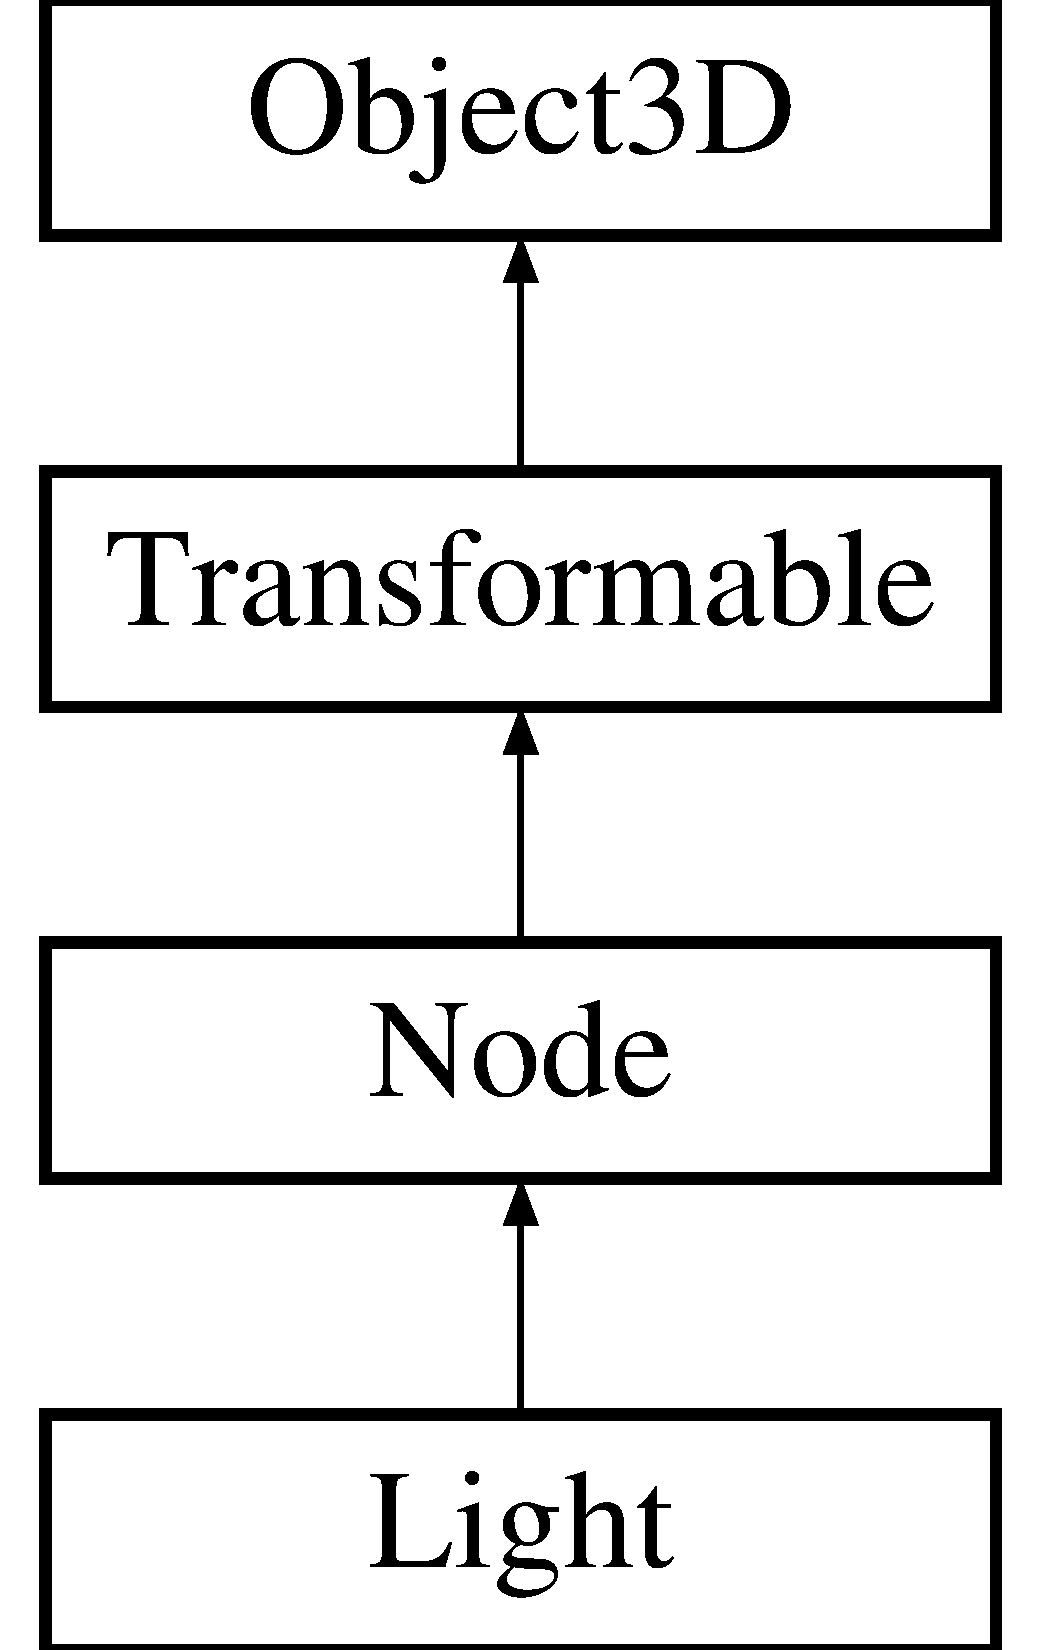
\includegraphics[height=5cm]{classm3g_1_1Light}
\end{center}
\end{figure}
\subsection*{Classes}
\begin{CompactItemize}
\item 
struct \hyperlink{structm3g_1_1Light_1_1Attenuation}{Attenuation}
\item 
struct \hyperlink{structm3g_1_1Light_1_1Spot}{Spot}
\end{CompactItemize}
\subsection*{Public Member Functions}
\begin{CompactItemize}
\item 
\hyperlink{classm3g_1_1Light_7f8a7be05225f470c200f7e4ff914a3c}{Light} ()
\item 
virtual \hyperlink{classm3g_1_1Light_f50d3d8cdb323e1a9fbd7bfac3aeba06}{$\sim$Light} ()
\item 
\hyperlink{classm3g_1_1Light}{Light} $\ast$ \hyperlink{classm3g_1_1Light_7a41af040d0c1566358d84f089cd0cd1}{duplicate} () const 
\item 
virtual void \hyperlink{classm3g_1_1Light_415c0b110f95410ded9b85e5d99a496b}{addAnimationTrack} (\hyperlink{classm3g_1_1AnimationTrack}{AnimationTrack} $\ast$animation\_\-track)
\item 
virtual int \hyperlink{classm3g_1_1Light_8aad1ceab4c2a03609c8a42324ce484d}{animate} (int world\_\-time)
\item 
int \hyperlink{classm3g_1_1Light_4cfa1931c265ec3412fe3f6408a1b4f5}{getColor} () const 
\item 
float \hyperlink{classm3g_1_1Light_9553ab96cb7639acafcebb81888af687}{getConstantAttenuation} () const 
\item 
float \hyperlink{classm3g_1_1Light_ca846da41d09a6ae01d6b362c33e938d}{getIntensity} () const 
\item 
float \hyperlink{classm3g_1_1Light_50e949b0cc2014e576987379cac07769}{getLinearAttenuation} () const 
\item 
int \hyperlink{classm3g_1_1Light_d4ce4524e4751fe5e3cfb8c270347d54}{getMode} () const 
\item 
float \hyperlink{classm3g_1_1Light_9ec7130ca1977cfeb4b2cbebc31971b4}{getQuadraticAttenuation} () const 
\item 
float \hyperlink{classm3g_1_1Light_1117f914d754fe74c090dc97bde905eb}{getSpotAngle} () const 
\item 
float \hyperlink{classm3g_1_1Light_a359fee191741efb7e576616a59a76f7}{getSpotExponent} () const 
\item 
void \hyperlink{classm3g_1_1Light_391c5cff137fc2e810f5129a5381196f}{setAttenuation} (float constant, float linear, float quadratic)
\item 
void \hyperlink{classm3g_1_1Light_b1f5cc0f5cc6bbbd716a526c61f1081d}{setColor} (int rgb)
\item 
void \hyperlink{classm3g_1_1Light_ce02325cb6289c007d569c193641c468}{setIntensity} (float intensity)
\item 
void \hyperlink{classm3g_1_1Light_9f407b18ba6235cb96fa95611c1ea3a4}{setMode} (int mode)
\item 
void \hyperlink{classm3g_1_1Light_30ce206b37f6ed5e918fbc75b3f91072}{setSpotAngle} (float angle)
\item 
void \hyperlink{classm3g_1_1Light_787eb66801e17d0412559598326ce19d}{setSpotExponent} (float exponent)
\item 
virtual std::ostream \& \hyperlink{classm3g_1_1Light_6fea17fa1532df3794f8cb39cb4f911f}{print} (std::ostream \&out) const 
\item 
virtual void \hyperlink{classm3g_1_1Light_8babc8a79b78615da51161e94029eea9}{render} (\hyperlink{structm3g_1_1RenderState}{RenderState} \&state) const 
\end{CompactItemize}
\subsection*{Public Attributes}
\begin{CompactItemize}
\item 
\hypertarget{classm3g_1_1Light_1ea5d0cb93f22f7d0fdf804bd68c3326}{
int \textbf{mode}}
\label{classm3g_1_1Light_1ea5d0cb93f22f7d0fdf804bd68c3326}

\item 
\hypertarget{classm3g_1_1Light_0fd02fb9277ffcb35a75066ffe95e8c7}{
int \textbf{color}}
\label{classm3g_1_1Light_0fd02fb9277ffcb35a75066ffe95e8c7}

\item 
\hypertarget{classm3g_1_1Light_299ec0c42ccc5a2d79d1739428ac3210}{
int \textbf{intensity}}
\label{classm3g_1_1Light_299ec0c42ccc5a2d79d1739428ac3210}

\item 
\hypertarget{classm3g_1_1Light_1569207c73e72f9b3ceeaba71b985378}{
\hyperlink{structm3g_1_1Light_1_1Attenuation}{Attenuation} \textbf{attenuation}}
\label{classm3g_1_1Light_1569207c73e72f9b3ceeaba71b985378}

\item 
\hypertarget{classm3g_1_1Light_8c48692471265603559309c9b2fd65a1}{
\hyperlink{structm3g_1_1Light_1_1Spot}{Spot} \textbf{spot}}
\label{classm3g_1_1Light_8c48692471265603559309c9b2fd65a1}

\end{CompactItemize}
\subsection*{Static Public Attributes}
\begin{CompactItemize}
\item 
static const int \hyperlink{classm3g_1_1Light_4cf648a82d9de62a1fb15f4277049594}{AMBIENT} = 128
\item 
static const int \hyperlink{classm3g_1_1Light_a2fb668ca8bbeb8323eda98fba594fda}{DIRECTIONAL} = 129
\item 
static const int \hyperlink{classm3g_1_1Light_34d360bb8395ad7fbcd3ec286ece64cb}{OMNI} = 130
\item 
static const int \hyperlink{classm3g_1_1Light_c44aef16b96dc8fd8b134416964a7de9}{SPOT} = 131
\end{CompactItemize}
\subsection*{Friends}
\begin{CompactItemize}
\item 
\hypertarget{classm3g_1_1Light_8174d4c629550c1ee279571250236ef4}{
class \textbf{Graphics3D}}
\label{classm3g_1_1Light_8174d4c629550c1ee279571250236ef4}

\item 
\hypertarget{classm3g_1_1Light_7b4bcdf992c21ae83363f25df05b1d25}{
class \textbf{World}}
\label{classm3g_1_1Light_7b4bcdf992c21ae83363f25df05b1d25}

\end{CompactItemize}


\subsection{Detailed Description}
A scene graph node that represents different kinds of light sources. 

\subsection{Constructor \& Destructor Documentation}
\hypertarget{classm3g_1_1Light_7f8a7be05225f470c200f7e4ff914a3c}{
\index{m3g::Light@{m3g::Light}!Light@{Light}}
\index{Light@{Light}!m3g::Light@{m3g::Light}}
\subsubsection[{Light}]{\setlength{\rightskip}{0pt plus 5cm}{\bf Light} ()}}
\label{classm3g_1_1Light_7f8a7be05225f470c200f7e4ff914a3c}


Consturct a new \hyperlink{classm3g_1_1Light}{Light} witdh default values. \hypertarget{classm3g_1_1Light_f50d3d8cdb323e1a9fbd7bfac3aeba06}{
\index{m3g::Light@{m3g::Light}!$\sim$Light@{$\sim$Light}}
\index{$\sim$Light@{$\sim$Light}!m3g::Light@{m3g::Light}}
\subsubsection[{$\sim$Light}]{\setlength{\rightskip}{0pt plus 5cm}$\sim${\bf Light} ()\hspace{0.3cm}{\tt  \mbox{[}virtual\mbox{]}}}}
\label{classm3g_1_1Light_f50d3d8cdb323e1a9fbd7bfac3aeba06}


Destruct this object. 

\subsection{Member Function Documentation}
\hypertarget{classm3g_1_1Light_415c0b110f95410ded9b85e5d99a496b}{
\index{m3g::Light@{m3g::Light}!addAnimationTrack@{addAnimationTrack}}
\index{addAnimationTrack@{addAnimationTrack}!m3g::Light@{m3g::Light}}
\subsubsection[{addAnimationTrack}]{\setlength{\rightskip}{0pt plus 5cm}void addAnimationTrack ({\bf AnimationTrack} $\ast$ {\em animation\_\-track})\hspace{0.3cm}{\tt  \mbox{[}virtual\mbox{]}}}}
\label{classm3g_1_1Light_415c0b110f95410ded9b85e5d99a496b}


Adds the given \hyperlink{classm3g_1_1AnimationTrack}{AnimationTrack} to this \hyperlink{classm3g_1_1Object3D}{Object3D}, 

Reimplemented from \hyperlink{classm3g_1_1Node_415c0b110f95410ded9b85e5d99a496b}{Node}.\hypertarget{classm3g_1_1Light_8aad1ceab4c2a03609c8a42324ce484d}{
\index{m3g::Light@{m3g::Light}!animate@{animate}}
\index{animate@{animate}!m3g::Light@{m3g::Light}}
\subsubsection[{animate}]{\setlength{\rightskip}{0pt plus 5cm}int animate (int {\em world\_\-time})\hspace{0.3cm}{\tt  \mbox{[}virtual\mbox{]}}}}
\label{classm3g_1_1Light_8aad1ceab4c2a03609c8a42324ce484d}


Updates all animated properties in this \hyperlink{classm3g_1_1Object3D}{Object3D} and all Object3Ds that are reachable from this \hyperlink{classm3g_1_1Object3D}{Object3D}. 

Reimplemented from \hyperlink{classm3g_1_1Node_8aad1ceab4c2a03609c8a42324ce484d}{Node}.\hypertarget{classm3g_1_1Light_7a41af040d0c1566358d84f089cd0cd1}{
\index{m3g::Light@{m3g::Light}!duplicate@{duplicate}}
\index{duplicate@{duplicate}!m3g::Light@{m3g::Light}}
\subsubsection[{duplicate}]{\setlength{\rightskip}{0pt plus 5cm}{\bf Light} $\ast$ duplicate () const\hspace{0.3cm}{\tt  \mbox{[}virtual\mbox{]}}}}
\label{classm3g_1_1Light_7a41af040d0c1566358d84f089cd0cd1}


Creates a duplicate of this \hyperlink{classm3g_1_1Object3D}{Object3D}. 

Reimplemented from \hyperlink{classm3g_1_1Node_0b9f7531a4b56d34f47aeb1fff0d37e0}{Node}.\hypertarget{classm3g_1_1Light_4cfa1931c265ec3412fe3f6408a1b4f5}{
\index{m3g::Light@{m3g::Light}!getColor@{getColor}}
\index{getColor@{getColor}!m3g::Light@{m3g::Light}}
\subsubsection[{getColor}]{\setlength{\rightskip}{0pt plus 5cm}int getColor () const}}
\label{classm3g_1_1Light_4cfa1931c265ec3412fe3f6408a1b4f5}


Retrieves the curent color fo this \hyperlink{classm3g_1_1Light}{Light}. \hypertarget{classm3g_1_1Light_9553ab96cb7639acafcebb81888af687}{
\index{m3g::Light@{m3g::Light}!getConstantAttenuation@{getConstantAttenuation}}
\index{getConstantAttenuation@{getConstantAttenuation}!m3g::Light@{m3g::Light}}
\subsubsection[{getConstantAttenuation}]{\setlength{\rightskip}{0pt plus 5cm}float getConstantAttenuation () const}}
\label{classm3g_1_1Light_9553ab96cb7639acafcebb81888af687}


Retrieves the current constant attenuation coefficient for this \hyperlink{classm3g_1_1Light}{Light}. \hypertarget{classm3g_1_1Light_ca846da41d09a6ae01d6b362c33e938d}{
\index{m3g::Light@{m3g::Light}!getIntensity@{getIntensity}}
\index{getIntensity@{getIntensity}!m3g::Light@{m3g::Light}}
\subsubsection[{getIntensity}]{\setlength{\rightskip}{0pt plus 5cm}float getIntensity () const}}
\label{classm3g_1_1Light_ca846da41d09a6ae01d6b362c33e938d}


Retrieves the current intensity of this \hyperlink{classm3g_1_1Light}{Light}. \hypertarget{classm3g_1_1Light_50e949b0cc2014e576987379cac07769}{
\index{m3g::Light@{m3g::Light}!getLinearAttenuation@{getLinearAttenuation}}
\index{getLinearAttenuation@{getLinearAttenuation}!m3g::Light@{m3g::Light}}
\subsubsection[{getLinearAttenuation}]{\setlength{\rightskip}{0pt plus 5cm}float getLinearAttenuation () const}}
\label{classm3g_1_1Light_50e949b0cc2014e576987379cac07769}


Retrieves the current linear attenuation coefficient for this \hyperlink{classm3g_1_1Light}{Light}. \hypertarget{classm3g_1_1Light_d4ce4524e4751fe5e3cfb8c270347d54}{
\index{m3g::Light@{m3g::Light}!getMode@{getMode}}
\index{getMode@{getMode}!m3g::Light@{m3g::Light}}
\subsubsection[{getMode}]{\setlength{\rightskip}{0pt plus 5cm}int getMode () const}}
\label{classm3g_1_1Light_d4ce4524e4751fe5e3cfb8c270347d54}


Retrieves the current type of this \hyperlink{classm3g_1_1Light}{Light}. \hypertarget{classm3g_1_1Light_9ec7130ca1977cfeb4b2cbebc31971b4}{
\index{m3g::Light@{m3g::Light}!getQuadraticAttenuation@{getQuadraticAttenuation}}
\index{getQuadraticAttenuation@{getQuadraticAttenuation}!m3g::Light@{m3g::Light}}
\subsubsection[{getQuadraticAttenuation}]{\setlength{\rightskip}{0pt plus 5cm}float getQuadraticAttenuation () const}}
\label{classm3g_1_1Light_9ec7130ca1977cfeb4b2cbebc31971b4}


Retrieves the current quadratic attenuation coefficient for this \hyperlink{classm3g_1_1Light}{Light}. \hypertarget{classm3g_1_1Light_1117f914d754fe74c090dc97bde905eb}{
\index{m3g::Light@{m3g::Light}!getSpotAngle@{getSpotAngle}}
\index{getSpotAngle@{getSpotAngle}!m3g::Light@{m3g::Light}}
\subsubsection[{getSpotAngle}]{\setlength{\rightskip}{0pt plus 5cm}float getSpotAngle () const}}
\label{classm3g_1_1Light_1117f914d754fe74c090dc97bde905eb}


Retrieves the current spot angle of this \hyperlink{classm3g_1_1Light}{Light}. \hypertarget{classm3g_1_1Light_a359fee191741efb7e576616a59a76f7}{
\index{m3g::Light@{m3g::Light}!getSpotExponent@{getSpotExponent}}
\index{getSpotExponent@{getSpotExponent}!m3g::Light@{m3g::Light}}
\subsubsection[{getSpotExponent}]{\setlength{\rightskip}{0pt plus 5cm}float getSpotExponent () const}}
\label{classm3g_1_1Light_a359fee191741efb7e576616a59a76f7}


Sets the spot exponent for this \hyperlink{classm3g_1_1Light}{Light}. \hypertarget{classm3g_1_1Light_6fea17fa1532df3794f8cb39cb4f911f}{
\index{m3g::Light@{m3g::Light}!print@{print}}
\index{print@{print}!m3g::Light@{m3g::Light}}
\subsubsection[{print}]{\setlength{\rightskip}{0pt plus 5cm}std::ostream \& print (std::ostream \& {\em out}) const\hspace{0.3cm}{\tt  \mbox{[}virtual\mbox{]}}}}
\label{classm3g_1_1Light_6fea17fa1532df3794f8cb39cb4f911f}


Print out information of this object, for debug only. 

Reimplemented from \hyperlink{classm3g_1_1Node_6fea17fa1532df3794f8cb39cb4f911f}{Node}.\hypertarget{classm3g_1_1Light_8babc8a79b78615da51161e94029eea9}{
\index{m3g::Light@{m3g::Light}!render@{render}}
\index{render@{render}!m3g::Light@{m3g::Light}}
\subsubsection[{render}]{\setlength{\rightskip}{0pt plus 5cm}void render ({\bf RenderState} \& {\em state}) const\hspace{0.3cm}{\tt  \mbox{[}virtual\mbox{]}}}}
\label{classm3g_1_1Light_8babc8a79b78615da51161e94029eea9}


Render this object, for inner use.

Note: \hyperlink{classm3g_1_1Light}{Light} should be rendered only at first rendering pass(pass=1). In other cases, do nothing. 

Reimplemented from \hyperlink{classm3g_1_1Node_8babc8a79b78615da51161e94029eea9}{Node}.\hypertarget{classm3g_1_1Light_391c5cff137fc2e810f5129a5381196f}{
\index{m3g::Light@{m3g::Light}!setAttenuation@{setAttenuation}}
\index{setAttenuation@{setAttenuation}!m3g::Light@{m3g::Light}}
\subsubsection[{setAttenuation}]{\setlength{\rightskip}{0pt plus 5cm}void setAttenuation (float {\em constant}, \/  float {\em linear}, \/  float {\em quadratic})}}
\label{classm3g_1_1Light_391c5cff137fc2e810f5129a5381196f}


Sets the attenuation coeffieicients for this \hyperlink{classm3g_1_1Light}{Light}. \hypertarget{classm3g_1_1Light_b1f5cc0f5cc6bbbd716a526c61f1081d}{
\index{m3g::Light@{m3g::Light}!setColor@{setColor}}
\index{setColor@{setColor}!m3g::Light@{m3g::Light}}
\subsubsection[{setColor}]{\setlength{\rightskip}{0pt plus 5cm}void setColor (int {\em rgb})}}
\label{classm3g_1_1Light_b1f5cc0f5cc6bbbd716a526c61f1081d}


Sets the color of this \hyperlink{classm3g_1_1Light}{Light}. \hypertarget{classm3g_1_1Light_ce02325cb6289c007d569c193641c468}{
\index{m3g::Light@{m3g::Light}!setIntensity@{setIntensity}}
\index{setIntensity@{setIntensity}!m3g::Light@{m3g::Light}}
\subsubsection[{setIntensity}]{\setlength{\rightskip}{0pt plus 5cm}void setIntensity (float {\em intensity})}}
\label{classm3g_1_1Light_ce02325cb6289c007d569c193641c468}


Sets the intensity of this \hyperlink{classm3g_1_1Light}{Light}. \hypertarget{classm3g_1_1Light_9f407b18ba6235cb96fa95611c1ea3a4}{
\index{m3g::Light@{m3g::Light}!setMode@{setMode}}
\index{setMode@{setMode}!m3g::Light@{m3g::Light}}
\subsubsection[{setMode}]{\setlength{\rightskip}{0pt plus 5cm}void setMode (int {\em mode})}}
\label{classm3g_1_1Light_9f407b18ba6235cb96fa95611c1ea3a4}


Sets the type of this \hyperlink{classm3g_1_1Light}{Light}. \hypertarget{classm3g_1_1Light_30ce206b37f6ed5e918fbc75b3f91072}{
\index{m3g::Light@{m3g::Light}!setSpotAngle@{setSpotAngle}}
\index{setSpotAngle@{setSpotAngle}!m3g::Light@{m3g::Light}}
\subsubsection[{setSpotAngle}]{\setlength{\rightskip}{0pt plus 5cm}void setSpotAngle (float {\em angle})}}
\label{classm3g_1_1Light_30ce206b37f6ed5e918fbc75b3f91072}


Sets the spot cone angle for this \hyperlink{classm3g_1_1Light}{Light}. \hypertarget{classm3g_1_1Light_787eb66801e17d0412559598326ce19d}{
\index{m3g::Light@{m3g::Light}!setSpotExponent@{setSpotExponent}}
\index{setSpotExponent@{setSpotExponent}!m3g::Light@{m3g::Light}}
\subsubsection[{setSpotExponent}]{\setlength{\rightskip}{0pt plus 5cm}void setSpotExponent (float {\em exponent})}}
\label{classm3g_1_1Light_787eb66801e17d0412559598326ce19d}


Sets the spot exponent for this \hyperlink{classm3g_1_1Light}{Light}. 

\subsection{Member Data Documentation}
\hypertarget{classm3g_1_1Light_4cf648a82d9de62a1fb15f4277049594}{
\index{m3g::Light@{m3g::Light}!AMBIENT@{AMBIENT}}
\index{AMBIENT@{AMBIENT}!m3g::Light@{m3g::Light}}
\subsubsection[{AMBIENT}]{\setlength{\rightskip}{0pt plus 5cm}const int {\bf AMBIENT} = 128\hspace{0.3cm}{\tt  \mbox{[}static\mbox{]}}}}
\label{classm3g_1_1Light_4cf648a82d9de62a1fb15f4277049594}


A paramter to setMode, specifying an amibent light source. \hypertarget{classm3g_1_1Light_a2fb668ca8bbeb8323eda98fba594fda}{
\index{m3g::Light@{m3g::Light}!DIRECTIONAL@{DIRECTIONAL}}
\index{DIRECTIONAL@{DIRECTIONAL}!m3g::Light@{m3g::Light}}
\subsubsection[{DIRECTIONAL}]{\setlength{\rightskip}{0pt plus 5cm}const int {\bf DIRECTIONAL} = 129\hspace{0.3cm}{\tt  \mbox{[}static\mbox{]}}}}
\label{classm3g_1_1Light_a2fb668ca8bbeb8323eda98fba594fda}


A paramter to setMode, specifying an directional light source. \hypertarget{classm3g_1_1Light_34d360bb8395ad7fbcd3ec286ece64cb}{
\index{m3g::Light@{m3g::Light}!OMNI@{OMNI}}
\index{OMNI@{OMNI}!m3g::Light@{m3g::Light}}
\subsubsection[{OMNI}]{\setlength{\rightskip}{0pt plus 5cm}const int {\bf OMNI} = 130\hspace{0.3cm}{\tt  \mbox{[}static\mbox{]}}}}
\label{classm3g_1_1Light_34d360bb8395ad7fbcd3ec286ece64cb}


A paramter to setMode, specifying an omnidirectional light source. \hypertarget{classm3g_1_1Light_c44aef16b96dc8fd8b134416964a7de9}{
\index{m3g::Light@{m3g::Light}!SPOT@{SPOT}}
\index{SPOT@{SPOT}!m3g::Light@{m3g::Light}}
\subsubsection[{SPOT}]{\setlength{\rightskip}{0pt plus 5cm}const int {\bf SPOT} = 131\hspace{0.3cm}{\tt  \mbox{[}static\mbox{]}}}}
\label{classm3g_1_1Light_c44aef16b96dc8fd8b134416964a7de9}


A paramter to setMode, specifying an spot light source. 

The documentation for this class was generated from the following files:\begin{CompactItemize}
\item 
/work/workspace.desktop-m3g/src/Light.hpp\item 
/work/workspace.desktop-m3g/src/Light.cpp\end{CompactItemize}

\hypertarget{classm3g_1_1Loader}{
\section{Loader Class Reference}
\label{classm3g_1_1Loader}\index{m3g::Loader@{m3g::Loader}}
}
{\tt \#include $<$Loader.hpp$>$}

\subsection*{Public Member Functions}
\begin{CompactItemize}
\item 
\hyperlink{classm3g_1_1Loader_c082256071478316a982894d4191a11a}{Loader} ()
\item 
\hyperlink{classm3g_1_1Loader_8bd25dd3f34914f06852c2de2f9db737}{$\sim$Loader} ()
\end{CompactItemize}
\subsection*{Static Public Member Functions}
\begin{CompactItemize}
\item 
static std::vector$<$ \hyperlink{classm3g_1_1Object3D}{Object3D} $\ast$ $>$ \hyperlink{classm3g_1_1Loader_7abddd36a9ee70e67de0e2183bba1aed}{load} (void $\ast$data, int offset)
\item 
static std::vector$<$ \hyperlink{classm3g_1_1Object3D}{Object3D} $\ast$ $>$ \hyperlink{classm3g_1_1Loader_27bd86888cdadd349223dcb303e45879}{load} (const char $\ast$name)
\end{CompactItemize}


\subsection{Detailed Description}
m3gファイルのローダー。インスタンス化不可. 

\subsection{Constructor \& Destructor Documentation}
\hypertarget{classm3g_1_1Loader_c082256071478316a982894d4191a11a}{
\index{m3g::Loader@{m3g::Loader}!Loader@{Loader}}
\index{Loader@{Loader}!m3g::Loader@{m3g::Loader}}
\subsubsection[{Loader}]{\setlength{\rightskip}{0pt plus 5cm}{\bf Loader} ()}}
\label{classm3g_1_1Loader_c082256071478316a982894d4191a11a}


コンストラクタ. \hypertarget{classm3g_1_1Loader_8bd25dd3f34914f06852c2de2f9db737}{
\index{m3g::Loader@{m3g::Loader}!$\sim$Loader@{$\sim$Loader}}
\index{$\sim$Loader@{$\sim$Loader}!m3g::Loader@{m3g::Loader}}
\subsubsection[{$\sim$Loader}]{\setlength{\rightskip}{0pt plus 5cm}$\sim${\bf Loader} ()}}
\label{classm3g_1_1Loader_8bd25dd3f34914f06852c2de2f9db737}


コンストラクタ.

デストラクタ. 

\subsection{Member Function Documentation}
\hypertarget{classm3g_1_1Loader_27bd86888cdadd349223dcb303e45879}{
\index{m3g::Loader@{m3g::Loader}!load@{load}}
\index{load@{load}!m3g::Loader@{m3g::Loader}}
\subsubsection[{load}]{\setlength{\rightskip}{0pt plus 5cm}std::vector$<$ {\bf Object3D} $\ast$ $>$ load (const char $\ast$ {\em name})\hspace{0.3cm}{\tt  \mbox{[}static\mbox{]}}}}
\label{classm3g_1_1Loader_27bd86888cdadd349223dcb303e45879}


与えられた名前のリソースからObject3Dのインスタンスを生成する. \hypertarget{classm3g_1_1Loader_7abddd36a9ee70e67de0e2183bba1aed}{
\index{m3g::Loader@{m3g::Loader}!load@{load}}
\index{load@{load}!m3g::Loader@{m3g::Loader}}
\subsubsection[{load}]{\setlength{\rightskip}{0pt plus 5cm}std::vector$<$ {\bf Object3D} $\ast$ $>$ load (void $\ast$ {\em data}, \/  int {\em offset})\hspace{0.3cm}{\tt  \mbox{[}static\mbox{]}}}}
\label{classm3g_1_1Loader_7abddd36a9ee70e67de0e2183bba1aed}


与えられたバイトストリームのオフセット位置からObject3Dのインスタンスを生成する. 

The documentation for this class was generated from the following files:\begin{CompactItemize}
\item 
/work/desktop-m3g/src/Loader.hpp\item 
/work/desktop-m3g/src/Loader.cpp\end{CompactItemize}

\hypertarget{classm3g_1_1Material}{
\section{Material Class Reference}
\label{classm3g_1_1Material}\index{m3g::Material@{m3g::Material}}
}
{\tt \#include $<$Material.hpp$>$}

Inheritance diagram for Material::\begin{figure}[H]
\begin{center}
\leavevmode
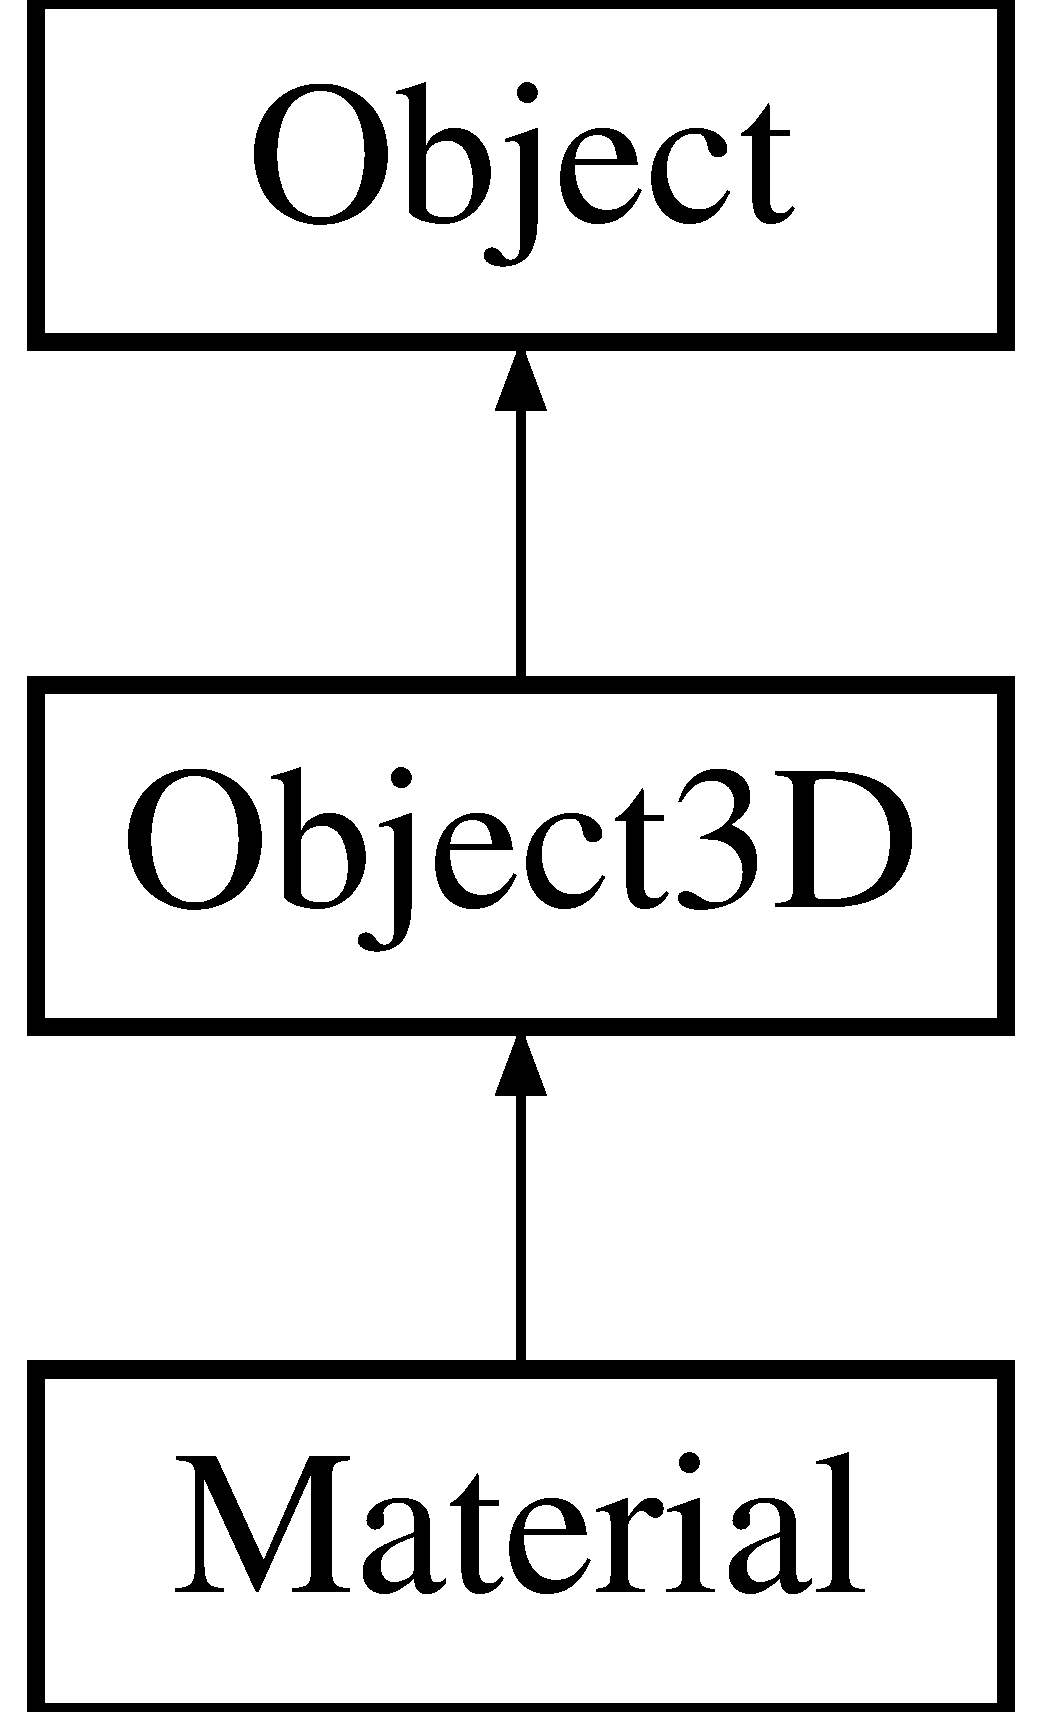
\includegraphics[height=3cm]{classm3g_1_1Material}
\end{center}
\end{figure}
\subsection*{Public Member Functions}
\begin{CompactItemize}
\item 
\hyperlink{classm3g_1_1Material_ade2019060d01e7983e9bc40ea6aa404}{Material} ()
\item 
virtual \hyperlink{classm3g_1_1Material_b15b7efa255e5cca9b02a031a783cfe8}{$\sim$Material} ()
\item 
virtual \hyperlink{classm3g_1_1Material}{Material} $\ast$ \hyperlink{classm3g_1_1Material_1bdbc2f934efac291bf7d8f49ba10dda}{duplicate} () const 
\item 
virtual void \hyperlink{classm3g_1_1Material_415c0b110f95410ded9b85e5d99a496b}{addAnimationTrack} (\hyperlink{classm3g_1_1AnimationTrack}{AnimationTrack} $\ast$animation\_\-track)
\item 
virtual int \hyperlink{classm3g_1_1Material_8aad1ceab4c2a03609c8a42324ce484d}{animate} (int world\_\-time)
\item 
int \hyperlink{classm3g_1_1Material_d5740043584c6bf87bf014402c5985be}{getColor} (int target) const 
\item 
float \hyperlink{classm3g_1_1Material_1bab082fe3510dbe7b98dd07b3976b5b}{getShininess} () const 
\item 
\hypertarget{classm3g_1_1Material_64fb5d60325fd073ab623d0eb04189d1}{
bool \textbf{isVertexColorTrackingEnabled} () const }
\label{classm3g_1_1Material_64fb5d60325fd073ab623d0eb04189d1}

\item 
void \hyperlink{classm3g_1_1Material_5947a525a18bca77aa890971df2ae48a}{setColor} (int target, int argb)
\item 
\hypertarget{classm3g_1_1Material_fb630e98bef48acb3b3c0541ed3615be}{
void \textbf{setShininess} (float shininess)}
\label{classm3g_1_1Material_fb630e98bef48acb3b3c0541ed3615be}

\item 
void \hyperlink{classm3g_1_1Material_55778ceeb6408e5db698c793dea1edd6}{setVertexColorTrackingEnable} (bool enable)
\item 
virtual std::ostream \& \hyperlink{classm3g_1_1Material_6fea17fa1532df3794f8cb39cb4f911f}{print} (std::ostream \&out) const 
\item 
virtual void \hyperlink{classm3g_1_1Material_8babc8a79b78615da51161e94029eea9}{render} (\hyperlink{structm3g_1_1RenderState}{RenderState} \&state) const 
\end{CompactItemize}
\subsection*{Static Public Member Functions}
\begin{CompactItemize}
\item 
static void \hyperlink{classm3g_1_1Material_443a7a301f77f625335ecc06d13bad06}{renderX} ()
\end{CompactItemize}
\subsection*{Static Public Attributes}
\begin{CompactItemize}
\item 
static const int \hyperlink{classm3g_1_1Material_4cf648a82d9de62a1fb15f4277049594}{AMBIENT} = 1$<$$<$10
\item 
static const int \hyperlink{classm3g_1_1Material_9798073e44254569f47464dc6bf5da89}{DIFFUSE} = 1$<$$<$11
\item 
static const int \hyperlink{classm3g_1_1Material_b92d57adf6955eae6adac15e865659cd}{EMISSIVE} = 1$<$$<$12
\item 
static const int \hyperlink{classm3g_1_1Material_cac20b25665d9a3713bec3a772a89ede}{SPECULAR} = 1$<$$<$13
\end{CompactItemize}
\subsection*{Friends}
\begin{CompactItemize}
\item 
\hypertarget{classm3g_1_1Material_afa5201a494f65c37039281d9b63a2a9}{
class \textbf{Appearance}}
\label{classm3g_1_1Material_afa5201a494f65c37039281d9b63a2a9}

\end{CompactItemize}


\subsection{Detailed Description}
An \hyperlink{classm3g_1_1Appearance}{Appearance} component encapsulating material attributes for lighting computations. 

\subsection{Constructor \& Destructor Documentation}
\hypertarget{classm3g_1_1Material_ade2019060d01e7983e9bc40ea6aa404}{
\index{m3g::Material@{m3g::Material}!Material@{Material}}
\index{Material@{Material}!m3g::Material@{m3g::Material}}
\subsubsection[{Material}]{\setlength{\rightskip}{0pt plus 5cm}{\bf Material} ()}}
\label{classm3g_1_1Material_ade2019060d01e7983e9bc40ea6aa404}


Creates a \hyperlink{classm3g_1_1Material}{Material} object with default values. \hypertarget{classm3g_1_1Material_b15b7efa255e5cca9b02a031a783cfe8}{
\index{m3g::Material@{m3g::Material}!$\sim$Material@{$\sim$Material}}
\index{$\sim$Material@{$\sim$Material}!m3g::Material@{m3g::Material}}
\subsubsection[{$\sim$Material}]{\setlength{\rightskip}{0pt plus 5cm}$\sim${\bf Material} ()\hspace{0.3cm}{\tt  \mbox{[}virtual\mbox{]}}}}
\label{classm3g_1_1Material_b15b7efa255e5cca9b02a031a783cfe8}


Destruct this object. 

\subsection{Member Function Documentation}
\hypertarget{classm3g_1_1Material_415c0b110f95410ded9b85e5d99a496b}{
\index{m3g::Material@{m3g::Material}!addAnimationTrack@{addAnimationTrack}}
\index{addAnimationTrack@{addAnimationTrack}!m3g::Material@{m3g::Material}}
\subsubsection[{addAnimationTrack}]{\setlength{\rightskip}{0pt plus 5cm}void addAnimationTrack ({\bf AnimationTrack} $\ast$ {\em animation\_\-track})\hspace{0.3cm}{\tt  \mbox{[}virtual\mbox{]}}}}
\label{classm3g_1_1Material_415c0b110f95410ded9b85e5d99a496b}


Adds the given \hyperlink{classm3g_1_1AnimationTrack}{AnimationTrack} to this \hyperlink{classm3g_1_1Object3D}{Object3D}, potentially changing the order and indices of the previously added tracks. 

Reimplemented from \hyperlink{classm3g_1_1Object3D_415c0b110f95410ded9b85e5d99a496b}{Object3D}.\hypertarget{classm3g_1_1Material_8aad1ceab4c2a03609c8a42324ce484d}{
\index{m3g::Material@{m3g::Material}!animate@{animate}}
\index{animate@{animate}!m3g::Material@{m3g::Material}}
\subsubsection[{animate}]{\setlength{\rightskip}{0pt plus 5cm}int animate (int {\em world\_\-time})\hspace{0.3cm}{\tt  \mbox{[}virtual\mbox{]}}}}
\label{classm3g_1_1Material_8aad1ceab4c2a03609c8a42324ce484d}


Update animatable property. 

Reimplemented from \hyperlink{classm3g_1_1Object3D_8aad1ceab4c2a03609c8a42324ce484d}{Object3D}.\hypertarget{classm3g_1_1Material_1bdbc2f934efac291bf7d8f49ba10dda}{
\index{m3g::Material@{m3g::Material}!duplicate@{duplicate}}
\index{duplicate@{duplicate}!m3g::Material@{m3g::Material}}
\subsubsection[{duplicate}]{\setlength{\rightskip}{0pt plus 5cm}{\bf Material} $\ast$ duplicate () const\hspace{0.3cm}{\tt  \mbox{[}virtual\mbox{]}}}}
\label{classm3g_1_1Material_1bdbc2f934efac291bf7d8f49ba10dda}


Creates a duplicate of this \hyperlink{classm3g_1_1Object3D}{Object3D}. 

Reimplemented from \hyperlink{classm3g_1_1Object3D_a25110dac934f867b83b73ad4741a0f4}{Object3D}.\hypertarget{classm3g_1_1Material_d5740043584c6bf87bf014402c5985be}{
\index{m3g::Material@{m3g::Material}!getColor@{getColor}}
\index{getColor@{getColor}!m3g::Material@{m3g::Material}}
\subsubsection[{getColor}]{\setlength{\rightskip}{0pt plus 5cm}int getColor (int {\em target}) const}}
\label{classm3g_1_1Material_d5740043584c6bf87bf014402c5985be}


Gets the value of the specified color component of this \hyperlink{classm3g_1_1Material}{Material}. \hypertarget{classm3g_1_1Material_1bab082fe3510dbe7b98dd07b3976b5b}{
\index{m3g::Material@{m3g::Material}!getShininess@{getShininess}}
\index{getShininess@{getShininess}!m3g::Material@{m3g::Material}}
\subsubsection[{getShininess}]{\setlength{\rightskip}{0pt plus 5cm}float getShininess () const}}
\label{classm3g_1_1Material_1bab082fe3510dbe7b98dd07b3976b5b}


Sets the shininess of this \hyperlink{classm3g_1_1Material}{Material}. \hypertarget{classm3g_1_1Material_6fea17fa1532df3794f8cb39cb4f911f}{
\index{m3g::Material@{m3g::Material}!print@{print}}
\index{print@{print}!m3g::Material@{m3g::Material}}
\subsubsection[{print}]{\setlength{\rightskip}{0pt plus 5cm}std::ostream \& print (std::ostream \& {\em out}) const\hspace{0.3cm}{\tt  \mbox{[}virtual\mbox{]}}}}
\label{classm3g_1_1Material_6fea17fa1532df3794f8cb39cb4f911f}


Print out information of this object, for debug only. 

Reimplemented from \hyperlink{classm3g_1_1Object3D_6fea17fa1532df3794f8cb39cb4f911f}{Object3D}.\hypertarget{classm3g_1_1Material_8babc8a79b78615da51161e94029eea9}{
\index{m3g::Material@{m3g::Material}!render@{render}}
\index{render@{render}!m3g::Material@{m3g::Material}}
\subsubsection[{render}]{\setlength{\rightskip}{0pt plus 5cm}void render ({\bf RenderState} \& {\em state}) const\hspace{0.3cm}{\tt  \mbox{[}virtual\mbox{]}}}}
\label{classm3g_1_1Material_8babc8a79b78615da51161e94029eea9}


Render this object, for inner use.

Note: \hyperlink{classm3g_1_1Material}{Material} should be rendered only at second rendering pass(pass=2). In other cases, do nothing. 

Reimplemented from \hyperlink{classm3g_1_1Object3D_8babc8a79b78615da51161e94029eea9}{Object3D}.\hypertarget{classm3g_1_1Material_443a7a301f77f625335ecc06d13bad06}{
\index{m3g::Material@{m3g::Material}!renderX@{renderX}}
\index{renderX@{renderX}!m3g::Material@{m3g::Material}}
\subsubsection[{renderX}]{\setlength{\rightskip}{0pt plus 5cm}void renderX ()\hspace{0.3cm}{\tt  \mbox{[}static\mbox{]}}}}
\label{classm3g_1_1Material_443a7a301f77f625335ecc06d13bad06}


Render this object, for inner use. \hypertarget{classm3g_1_1Material_5947a525a18bca77aa890971df2ae48a}{
\index{m3g::Material@{m3g::Material}!setColor@{setColor}}
\index{setColor@{setColor}!m3g::Material@{m3g::Material}}
\subsubsection[{setColor}]{\setlength{\rightskip}{0pt plus 5cm}void setColor (int {\em target}, \/  int {\em argb})}}
\label{classm3g_1_1Material_5947a525a18bca77aa890971df2ae48a}


Sets the given value to the specified color component(s) of this \hyperlink{classm3g_1_1Material}{Material}. \hypertarget{classm3g_1_1Material_55778ceeb6408e5db698c793dea1edd6}{
\index{m3g::Material@{m3g::Material}!setVertexColorTrackingEnable@{setVertexColorTrackingEnable}}
\index{setVertexColorTrackingEnable@{setVertexColorTrackingEnable}!m3g::Material@{m3g::Material}}
\subsubsection[{setVertexColorTrackingEnable}]{\setlength{\rightskip}{0pt plus 5cm}void setVertexColorTrackingEnable (bool {\em enable})}}
\label{classm3g_1_1Material_55778ceeb6408e5db698c793dea1edd6}


Enables or disables vertex color tracking. 

\subsection{Member Data Documentation}
\hypertarget{classm3g_1_1Material_4cf648a82d9de62a1fb15f4277049594}{
\index{m3g::Material@{m3g::Material}!AMBIENT@{AMBIENT}}
\index{AMBIENT@{AMBIENT}!m3g::Material@{m3g::Material}}
\subsubsection[{AMBIENT}]{\setlength{\rightskip}{0pt plus 5cm}const int {\bf AMBIENT} = 1$<$$<$10\hspace{0.3cm}{\tt  \mbox{[}static\mbox{]}}}}
\label{classm3g_1_1Material_4cf648a82d9de62a1fb15f4277049594}


A parameter to setColor and getColor, specifying that the ambient color component. \hypertarget{classm3g_1_1Material_9798073e44254569f47464dc6bf5da89}{
\index{m3g::Material@{m3g::Material}!DIFFUSE@{DIFFUSE}}
\index{DIFFUSE@{DIFFUSE}!m3g::Material@{m3g::Material}}
\subsubsection[{DIFFUSE}]{\setlength{\rightskip}{0pt plus 5cm}const int {\bf DIFFUSE} = 1$<$$<$11\hspace{0.3cm}{\tt  \mbox{[}static\mbox{]}}}}
\label{classm3g_1_1Material_9798073e44254569f47464dc6bf5da89}


A parameter to setColor and getColor, specifying that the diffuse color component. \hypertarget{classm3g_1_1Material_b92d57adf6955eae6adac15e865659cd}{
\index{m3g::Material@{m3g::Material}!EMISSIVE@{EMISSIVE}}
\index{EMISSIVE@{EMISSIVE}!m3g::Material@{m3g::Material}}
\subsubsection[{EMISSIVE}]{\setlength{\rightskip}{0pt plus 5cm}const int {\bf EMISSIVE} = 1$<$$<$12\hspace{0.3cm}{\tt  \mbox{[}static\mbox{]}}}}
\label{classm3g_1_1Material_b92d57adf6955eae6adac15e865659cd}


A parameter to setColor and getColor, specifying that the emissive color component. \hypertarget{classm3g_1_1Material_cac20b25665d9a3713bec3a772a89ede}{
\index{m3g::Material@{m3g::Material}!SPECULAR@{SPECULAR}}
\index{SPECULAR@{SPECULAR}!m3g::Material@{m3g::Material}}
\subsubsection[{SPECULAR}]{\setlength{\rightskip}{0pt plus 5cm}const int {\bf SPECULAR} = 1$<$$<$13\hspace{0.3cm}{\tt  \mbox{[}static\mbox{]}}}}
\label{classm3g_1_1Material_cac20b25665d9a3713bec3a772a89ede}


A parameter to setColor and getColor, specifying that the specular color component. 

The documentation for this class was generated from the following files:\begin{CompactItemize}
\item 
/work/workspace.desktop-m3g/src/Material.hpp\item 
/work/workspace.desktop-m3g/src/Material.cpp\end{CompactItemize}

\hypertarget{classm3g_1_1Matrix}{
\section{Matrix Class Reference}
\label{classm3g_1_1Matrix}\index{m3g::Matrix@{m3g::Matrix}}
}
{\tt \#include $<$Matrix.hpp$>$}

\subsection*{Public Member Functions}
\begin{CompactItemize}
\item 
\hypertarget{classm3g_1_1Matrix_04fd433badb74a2d60395217701d4009}{
\textbf{Matrix} (float $\ast$m4x4)}
\label{classm3g_1_1Matrix_04fd433badb74a2d60395217701d4009}

\item 
\hypertarget{classm3g_1_1Matrix_2c2f600f3a4c1db4a0da0b57db8aebca}{
\textbf{Matrix} (float m00, float m01, float m02, float m03, float m10, float m11, float m12, float m13, float m20, float m21, float m22, float m23, float m30, float m31, float m32, float m33)}
\label{classm3g_1_1Matrix_2c2f600f3a4c1db4a0da0b57db8aebca}

\item 
\hypertarget{classm3g_1_1Matrix_ed427d2cd38fe4a0b23f7f80803b7fd5}{
void \textbf{set} (const float $\ast$mat)}
\label{classm3g_1_1Matrix_ed427d2cd38fe4a0b23f7f80803b7fd5}

\item 
\hypertarget{classm3g_1_1Matrix_382e6ad7e6721b121e510959e1011be3}{
void \textbf{setIdentity} ()}
\label{classm3g_1_1Matrix_382e6ad7e6721b121e510959e1011be3}

\item 
\hypertarget{classm3g_1_1Matrix_c4e04770db1fedff14c37b5e4e4a68c6}{
void \textbf{setRotate} (float angle, float ax, float ay, float az)}
\label{classm3g_1_1Matrix_c4e04770db1fedff14c37b5e4e4a68c6}

\item 
\hypertarget{classm3g_1_1Matrix_937d04042c25021532ea2532fe5e3a32}{
void \textbf{setScale} (float sx, float sy, float sz)}
\label{classm3g_1_1Matrix_937d04042c25021532ea2532fe5e3a32}

\item 
\hypertarget{classm3g_1_1Matrix_550cf39dca5ec8d74d719b0dcdecdd4b}{
void \textbf{setTranslate} (float tx, float ty, float tz)}
\label{classm3g_1_1Matrix_550cf39dca5ec8d74d719b0dcdecdd4b}

\item 
\hypertarget{classm3g_1_1Matrix_7fa1616cc61c19a5efcc863c950f7f30}{
void \textbf{invert} ()}
\label{classm3g_1_1Matrix_7fa1616cc61c19a5efcc863c950f7f30}

\item 
\hypertarget{classm3g_1_1Matrix_f3a99ffb20127be48232d12260e934dc}{
void \textbf{transpose} ()}
\label{classm3g_1_1Matrix_f3a99ffb20127be48232d12260e934dc}

\item 
\hypertarget{classm3g_1_1Matrix_5d28596666a27f88d74bacceaef9b326}{
\hyperlink{classm3g_1_1Matrix}{Matrix} \& \textbf{operator$\ast$=} (const \hyperlink{classm3g_1_1Matrix}{Matrix} \&rhs)}
\label{classm3g_1_1Matrix_5d28596666a27f88d74bacceaef9b326}

\item 
std::ostream \& \hyperlink{classm3g_1_1Matrix_6fea17fa1532df3794f8cb39cb4f911f}{print} (std::ostream \&out) const 
\end{CompactItemize}
\subsection*{Public Attributes}
\begin{CompactItemize}
\item 
\hypertarget{classm3g_1_1Matrix_7cdab8754cd800b1ba4008e559aa314c}{
float \textbf{m} \mbox{[}4\mbox{]}\mbox{[}4\mbox{]}}
\label{classm3g_1_1Matrix_7cdab8754cd800b1ba4008e559aa314c}

\end{CompactItemize}


\subsection{Detailed Description}
行列クラス。内部使用専用. 

\subsection{Member Function Documentation}
\hypertarget{classm3g_1_1Matrix_6fea17fa1532df3794f8cb39cb4f911f}{
\index{m3g::Matrix@{m3g::Matrix}!print@{print}}
\index{print@{print}!m3g::Matrix@{m3g::Matrix}}
\subsubsection[{print}]{\setlength{\rightskip}{0pt plus 5cm}std::ostream \& print (std::ostream \& {\em out}) const}}
\label{classm3g_1_1Matrix_6fea17fa1532df3794f8cb39cb4f911f}


このMatrixクラスの情報を表示する。デバッグ用. 

The documentation for this class was generated from the following files:\begin{CompactItemize}
\item 
/work/desktop-m3g/src/Matrix.hpp\item 
/work/desktop-m3g/src/Matrix.cpp\end{CompactItemize}

\hypertarget{classm3g_1_1Mesh}{
\section{クラス Mesh}
\label{classm3g_1_1Mesh}\index{m3g::Mesh@{m3g::Mesh}}
}
{\tt \#include $<$Mesh.hpp$>$}

Meshに対する継承グラフ:\begin{figure}[H]
\begin{center}
\leavevmode
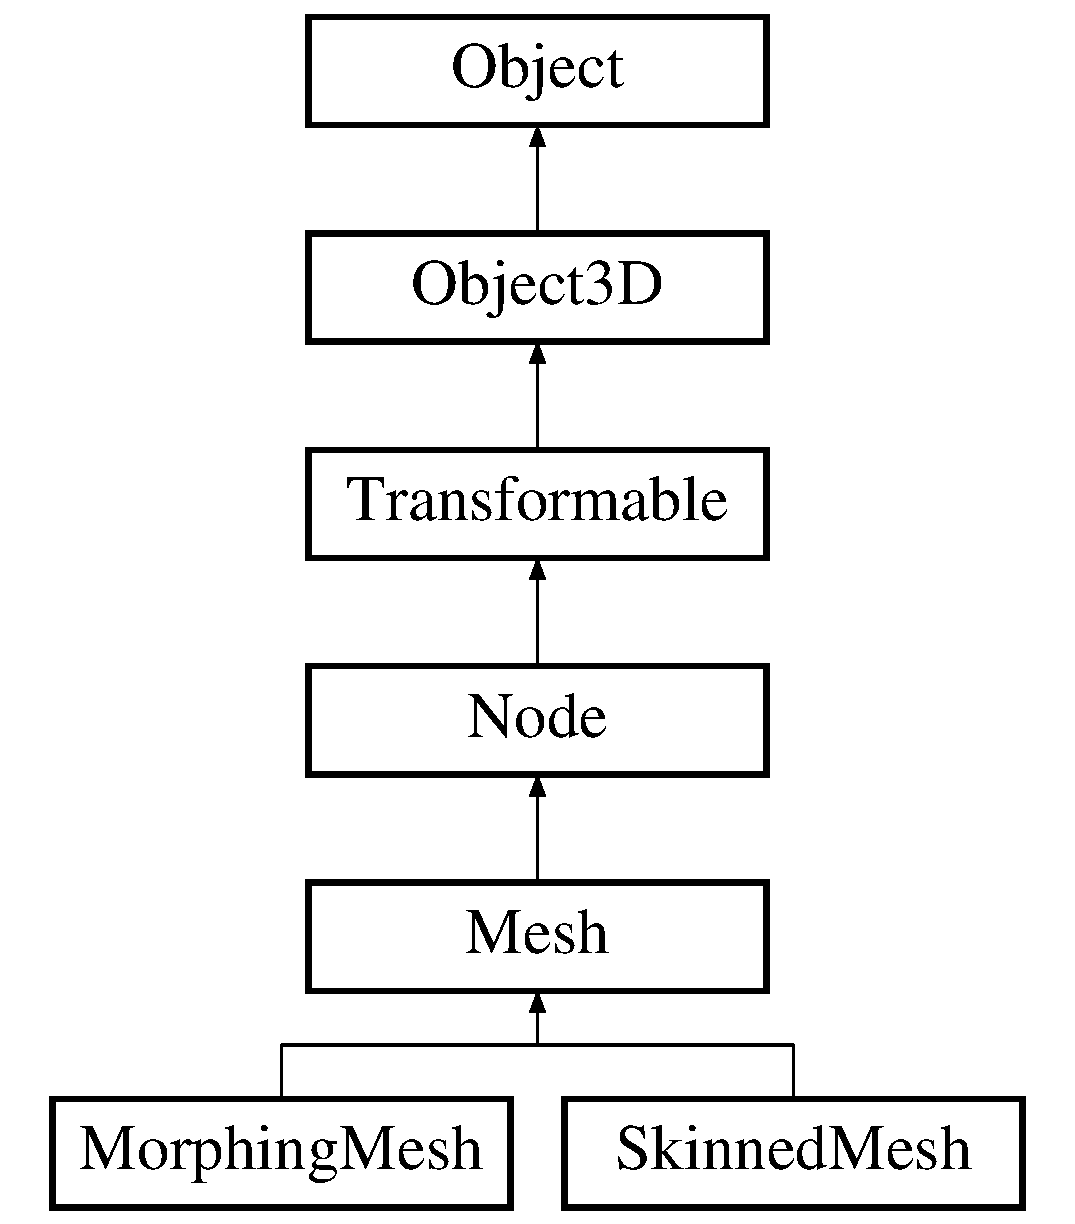
\includegraphics[height=5cm]{classm3g_1_1Mesh}
\end{center}
\end{figure}
\subsection*{Public メソッド}
\begin{CompactItemize}
\item 
\hyperlink{classm3g_1_1Mesh_2545f0abeee27d408d3129f3a5df40bb}{Mesh} (\hyperlink{classm3g_1_1VertexBuffer}{VertexBuffer} $\ast$vertices, int num\_\-submesh, \hyperlink{classm3g_1_1IndexBuffer}{IndexBuffer} $\ast$$\ast$submeshes, int num\_\-appearance, \hyperlink{classm3g_1_1Appearance}{Appearance} $\ast$$\ast$appearances)
\item 
\hyperlink{classm3g_1_1Mesh_2d7766ebbb63eccd77d0dd8b53b400a3}{Mesh} (\hyperlink{classm3g_1_1VertexBuffer}{VertexBuffer} $\ast$vertices, \hyperlink{classm3g_1_1IndexBuffer}{IndexBuffer} $\ast$submesh, \hyperlink{classm3g_1_1Appearance}{Appearance} $\ast$appearance)
\item 
virtual \hyperlink{classm3g_1_1Mesh_6e26384cfb03023e7dc2e5419baf813f}{$\sim$Mesh} ()
\item 
virtual int \hyperlink{classm3g_1_1Mesh_82cfeb67ca66b93e2ca7bda9a4f0e2aa}{animate} (int time)
\item 
\hyperlink{classm3g_1_1Appearance}{Appearance} $\ast$ \hyperlink{classm3g_1_1Mesh_4950a19e02c022dcf41a086117eb8219}{getAppearance} (int index) const 
\item 
\hyperlink{classm3g_1_1IndexBuffer}{IndexBuffer} $\ast$ \hyperlink{classm3g_1_1Mesh_ca34a663f46ce20e2b894c046714ea1d}{getIndexBuffer} (int index) const 
\item 
int \hyperlink{classm3g_1_1Mesh_5dc5a57ad549eb97504c2a1280a882dd}{getSubmeshCount} () const 
\item 
\hyperlink{classm3g_1_1VertexBuffer}{VertexBuffer} $\ast$ \hyperlink{classm3g_1_1Mesh_7602e9bf450fa8b3ec3c60e2e88cba25}{getVertexBuffer} () const 
\item 
void \hyperlink{classm3g_1_1Mesh_bb03b872c453c4f8f3fe31e8b54d1b52}{setAppearance} (int index, \hyperlink{classm3g_1_1Appearance}{Appearance} $\ast$appearance)
\item 
virtual std::ostream \& \hyperlink{classm3g_1_1Mesh_6fea17fa1532df3794f8cb39cb4f911f}{print} (std::ostream \&out) const 
\end{CompactItemize}
\subsection*{Protected メソッド}
\begin{CompactItemize}
\item 
virtual void \hyperlink{classm3g_1_1Mesh_1efcb1973989d9963d5bd6d03065d389}{render} (int pass, int index=0) const 
\end{CompactItemize}
\subsection*{Protected 変数}
\begin{CompactItemize}
\item 
\hypertarget{classm3g_1_1Mesh_1a2db0a8bc6986ba148b6b6f5dee271f}{
\hyperlink{classm3g_1_1VertexBuffer}{VertexBuffer} $\ast$ \textbf{vertices}}
\label{classm3g_1_1Mesh_1a2db0a8bc6986ba148b6b6f5dee271f}

\item 
\hypertarget{classm3g_1_1Mesh_7280e670882c2ce658bd600655fb477e}{
std::vector$<$ \hyperlink{classm3g_1_1IndexBuffer}{IndexBuffer} $\ast$ $>$ \textbf{indices}}
\label{classm3g_1_1Mesh_7280e670882c2ce658bd600655fb477e}

\item 
\hypertarget{classm3g_1_1Mesh_6dcb9adb660a04b601286a3ce4500fba}{
std::vector$<$ \hyperlink{classm3g_1_1Appearance}{Appearance} $\ast$ $>$ \textbf{appearances}}
\label{classm3g_1_1Mesh_6dcb9adb660a04b601286a3ce4500fba}

\end{CompactItemize}


\subsection{説明}
ポリゴナルサーフェスを定義するシーングラフのノード. 

\subsection{コンストラクタとデストラクタ}
\hypertarget{classm3g_1_1Mesh_2545f0abeee27d408d3129f3a5df40bb}{
\index{m3g::Mesh@{m3g::Mesh}!Mesh@{Mesh}}
\index{Mesh@{Mesh}!m3g::Mesh@{m3g::Mesh}}
\subsubsection[{Mesh}]{\setlength{\rightskip}{0pt plus 5cm}{\bf Mesh} ({\bf VertexBuffer} $\ast$ {\em vertices}, \/  int {\em num\_\-submesh}, \/  {\bf IndexBuffer} $\ast$$\ast$ {\em submeshes}, \/  int {\em num\_\-appearance}, \/  {\bf Appearance} $\ast$$\ast$ {\em appearances})}}
\label{classm3g_1_1Mesh_2545f0abeee27d408d3129f3a5df40bb}


指定された頂点バッファーとサブメッシュから新しいメッシュを作成する. \hypertarget{classm3g_1_1Mesh_2d7766ebbb63eccd77d0dd8b53b400a3}{
\index{m3g::Mesh@{m3g::Mesh}!Mesh@{Mesh}}
\index{Mesh@{Mesh}!m3g::Mesh@{m3g::Mesh}}
\subsubsection[{Mesh}]{\setlength{\rightskip}{0pt plus 5cm}{\bf Mesh} ({\bf VertexBuffer} $\ast$ {\em vertices}, \/  {\bf IndexBuffer} $\ast$ {\em submesh}, \/  {\bf Appearance} $\ast$ {\em appearance})}}
\label{classm3g_1_1Mesh_2d7766ebbb63eccd77d0dd8b53b400a3}


サブメッシュ1つからなる新しいメッシュを作成する. \hypertarget{classm3g_1_1Mesh_6e26384cfb03023e7dc2e5419baf813f}{
\index{m3g::Mesh@{m3g::Mesh}!$\sim$Mesh@{$\sim$Mesh}}
\index{$\sim$Mesh@{$\sim$Mesh}!m3g::Mesh@{m3g::Mesh}}
\subsubsection[{$\sim$Mesh}]{\setlength{\rightskip}{0pt plus 5cm}$\sim${\bf Mesh} ()\hspace{0.3cm}{\tt  \mbox{[}virtual\mbox{]}}}}
\label{classm3g_1_1Mesh_6e26384cfb03023e7dc2e5419baf813f}


このオブジェクトを削除するデストラクタ. 

\subsection{関数}
\hypertarget{classm3g_1_1Mesh_82cfeb67ca66b93e2ca7bda9a4f0e2aa}{
\index{m3g::Mesh@{m3g::Mesh}!animate@{animate}}
\index{animate@{animate}!m3g::Mesh@{m3g::Mesh}}
\subsubsection[{animate}]{\setlength{\rightskip}{0pt plus 5cm}int animate (int {\em time})\hspace{0.3cm}{\tt  \mbox{[}virtual\mbox{]}}}}
\label{classm3g_1_1Mesh_82cfeb67ca66b93e2ca7bda9a4f0e2aa}


このObject3D自身とここから到達できるObject3Dのアニメーテッドプロパティを更新する. 

\hyperlink{classm3g_1_1Node_8aad1ceab4c2a03609c8a42324ce484d}{Node}を再定義しています。

\hyperlink{classm3g_1_1MorphingMesh_8aad1ceab4c2a03609c8a42324ce484d}{MorphingMesh}で再定義されています。\hypertarget{classm3g_1_1Mesh_4950a19e02c022dcf41a086117eb8219}{
\index{m3g::Mesh@{m3g::Mesh}!getAppearance@{getAppearance}}
\index{getAppearance@{getAppearance}!m3g::Mesh@{m3g::Mesh}}
\subsubsection[{getAppearance}]{\setlength{\rightskip}{0pt plus 5cm}{\bf Appearance} $\ast$ getAppearance (int {\em index}) const}}
\label{classm3g_1_1Mesh_4950a19e02c022dcf41a086117eb8219}


指定されたサブメッシュのカレントのアピアランスを取得. \hypertarget{classm3g_1_1Mesh_ca34a663f46ce20e2b894c046714ea1d}{
\index{m3g::Mesh@{m3g::Mesh}!getIndexBuffer@{getIndexBuffer}}
\index{getIndexBuffer@{getIndexBuffer}!m3g::Mesh@{m3g::Mesh}}
\subsubsection[{getIndexBuffer}]{\setlength{\rightskip}{0pt plus 5cm}{\bf IndexBuffer} $\ast$ getIndexBuffer (int {\em index}) const}}
\label{classm3g_1_1Mesh_ca34a663f46ce20e2b894c046714ea1d}


指定されたインデックスのサブメッシュを取得. \hypertarget{classm3g_1_1Mesh_5dc5a57ad549eb97504c2a1280a882dd}{
\index{m3g::Mesh@{m3g::Mesh}!getSubmeshCount@{getSubmeshCount}}
\index{getSubmeshCount@{getSubmeshCount}!m3g::Mesh@{m3g::Mesh}}
\subsubsection[{getSubmeshCount}]{\setlength{\rightskip}{0pt plus 5cm}int getSubmeshCount () const}}
\label{classm3g_1_1Mesh_5dc5a57ad549eb97504c2a1280a882dd}


このメッシュのサブメッシュ数を取得. \hypertarget{classm3g_1_1Mesh_7602e9bf450fa8b3ec3c60e2e88cba25}{
\index{m3g::Mesh@{m3g::Mesh}!getVertexBuffer@{getVertexBuffer}}
\index{getVertexBuffer@{getVertexBuffer}!m3g::Mesh@{m3g::Mesh}}
\subsubsection[{getVertexBuffer}]{\setlength{\rightskip}{0pt plus 5cm}{\bf VertexBuffer} $\ast$ getVertexBuffer () const}}
\label{classm3g_1_1Mesh_7602e9bf450fa8b3ec3c60e2e88cba25}


このメッシュの頂点バッファーの取得. \hypertarget{classm3g_1_1Mesh_6fea17fa1532df3794f8cb39cb4f911f}{
\index{m3g::Mesh@{m3g::Mesh}!print@{print}}
\index{print@{print}!m3g::Mesh@{m3g::Mesh}}
\subsubsection[{print}]{\setlength{\rightskip}{0pt plus 5cm}std::ostream \& print (std::ostream \& {\em out}) const\hspace{0.3cm}{\tt  \mbox{[}virtual\mbox{]}}}}
\label{classm3g_1_1Mesh_6fea17fa1532df3794f8cb39cb4f911f}


このMeshクラスの情報を表示する。デバッグ用. 

\hyperlink{classm3g_1_1Node_6fea17fa1532df3794f8cb39cb4f911f}{Node}を再定義しています。

\hyperlink{classm3g_1_1MorphingMesh_6fea17fa1532df3794f8cb39cb4f911f}{MorphingMesh}, と \hyperlink{classm3g_1_1SkinnedMesh_6fea17fa1532df3794f8cb39cb4f911f}{SkinnedMesh}で再定義されています。\hypertarget{classm3g_1_1Mesh_1efcb1973989d9963d5bd6d03065d389}{
\index{m3g::Mesh@{m3g::Mesh}!render@{render}}
\index{render@{render}!m3g::Mesh@{m3g::Mesh}}
\subsubsection[{render}]{\setlength{\rightskip}{0pt plus 5cm}void render (int {\em pass}, \/  int {\em index} = {\tt 0}) const\hspace{0.3cm}{\tt  \mbox{[}protected, virtual\mbox{]}}}}
\label{classm3g_1_1Mesh_1efcb1973989d9963d5bd6d03065d389}


このノードをレンダリングする内部使用の関数.

Note: \hyperlink{classm3g_1_1Mesh}{Mesh} should be rendered only at second rendering pass(pass=2). In other cases, do nothing. 

\hyperlink{classm3g_1_1Node_1efcb1973989d9963d5bd6d03065d389}{Node}を再定義しています。

\hyperlink{classm3g_1_1MorphingMesh_1efcb1973989d9963d5bd6d03065d389}{MorphingMesh}, と \hyperlink{classm3g_1_1SkinnedMesh_1efcb1973989d9963d5bd6d03065d389}{SkinnedMesh}で再定義されています。\hypertarget{classm3g_1_1Mesh_bb03b872c453c4f8f3fe31e8b54d1b52}{
\index{m3g::Mesh@{m3g::Mesh}!setAppearance@{setAppearance}}
\index{setAppearance@{setAppearance}!m3g::Mesh@{m3g::Mesh}}
\subsubsection[{setAppearance}]{\setlength{\rightskip}{0pt plus 5cm}void setAppearance (int {\em index}, \/  {\bf Appearance} $\ast$ {\em appearance})}}
\label{classm3g_1_1Mesh_bb03b872c453c4f8f3fe31e8b54d1b52}


指定されたサブメッシュのアピアランスを設定. 

このクラスの説明は次のファイルから生成されました:\begin{CompactItemize}
\item 
/work/desktop-m3g/src/Mesh.hpp\item 
/work/desktop-m3g/src/Mesh.cpp\end{CompactItemize}

\hypertarget{classm3g_1_1MorphingMesh}{
\section{クラス MorphingMesh}
\label{classm3g_1_1MorphingMesh}\index{m3g::MorphingMesh@{m3g::MorphingMesh}}
}
{\tt \#include $<$MorphingMesh.hpp$>$}

MorphingMeshに対する継承グラフ:\begin{figure}[H]
\begin{center}
\leavevmode
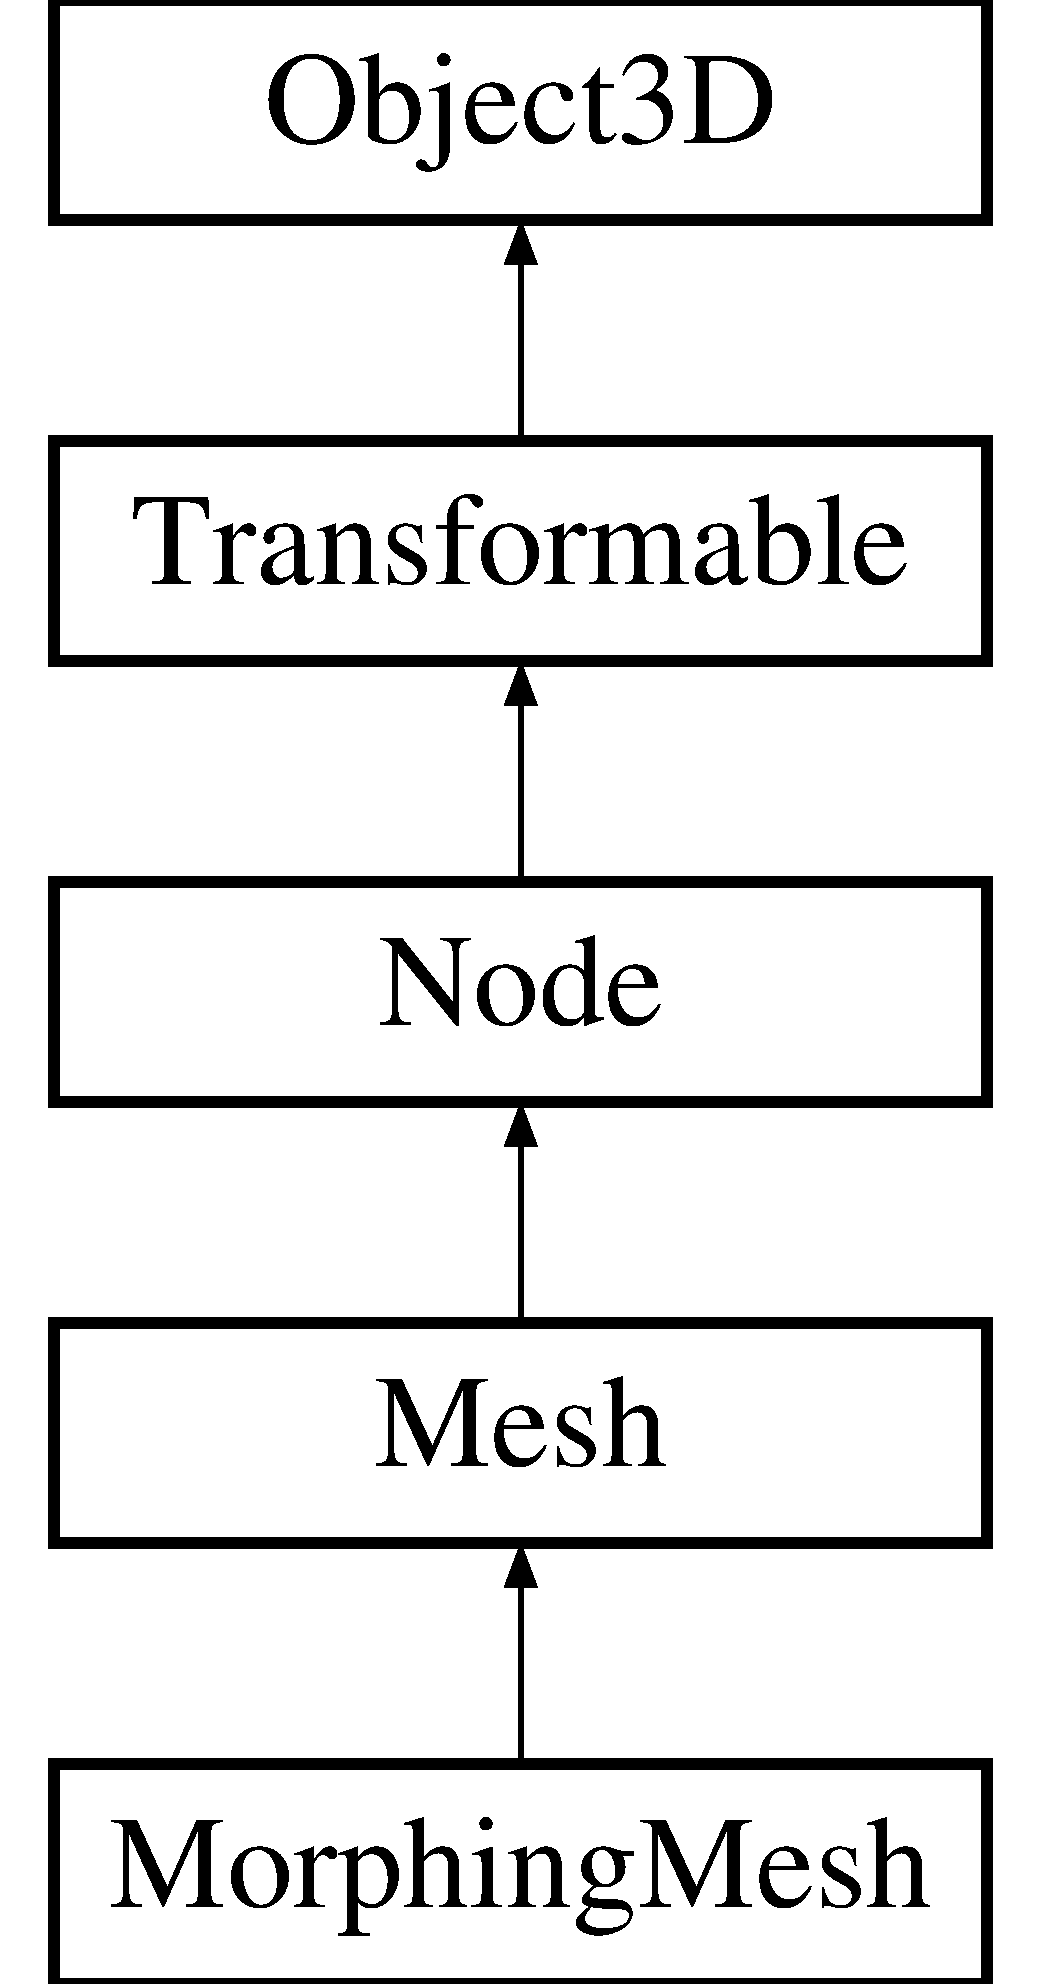
\includegraphics[height=6cm]{classm3g_1_1MorphingMesh}
\end{center}
\end{figure}
\subsection*{Public メソッド}
\begin{CompactItemize}
\item 
\hyperlink{classm3g_1_1MorphingMesh_211192cdba0b1d136977403ba4ed0d0c}{MorphingMesh} (\hyperlink{classm3g_1_1VertexBuffer}{VertexBuffer} $\ast$base, int num\_\-target, \hyperlink{classm3g_1_1VertexBuffer}{VertexBuffer} $\ast$$\ast$targets, int num\_\-submesh, \hyperlink{classm3g_1_1IndexBuffer}{IndexBuffer} $\ast$$\ast$submeshes, \hyperlink{classm3g_1_1Appearance}{Appearance} $\ast$$\ast$appearances)
\item 
\hyperlink{classm3g_1_1MorphingMesh_4a2347ee9c813fa1a6eef998f37bf6d5}{MorphingMesh} (\hyperlink{classm3g_1_1VertexBuffer}{VertexBuffer} $\ast$base, int num\_\-target, \hyperlink{classm3g_1_1VertexBuffer}{VertexBuffer} $\ast$$\ast$targets, \hyperlink{classm3g_1_1IndexBuffer}{IndexBuffer} $\ast$submesh, \hyperlink{classm3g_1_1Appearance}{Appearance} $\ast$appearance)
\item 
virtual \hyperlink{classm3g_1_1MorphingMesh_cdafafba64a0167f28f3b66ac4b9d7d6}{$\sim$MorphingMesh} ()
\item 
virtual \hyperlink{classm3g_1_1MorphingMesh}{MorphingMesh} $\ast$ \hyperlink{classm3g_1_1MorphingMesh_7e7b2c3c4c988c6341a5e249bd468f57}{duplicate} () const 
\item 
virtual int \hyperlink{classm3g_1_1MorphingMesh_8aad1ceab4c2a03609c8a42324ce484d}{animate} (int world\_\-time)
\item 
virtual void \hyperlink{classm3g_1_1MorphingMesh_415c0b110f95410ded9b85e5d99a496b}{addAnimationTrack} (\hyperlink{classm3g_1_1AnimationTrack}{AnimationTrack} $\ast$animation\_\-track)
\item 
\hyperlink{classm3g_1_1VertexBuffer}{VertexBuffer} $\ast$ \hyperlink{classm3g_1_1MorphingMesh_44766cc08b595f074d0d698c75f544b4}{getMorphTarget} (int index) const 
\item 
int \hyperlink{classm3g_1_1MorphingMesh_620d9684124201f738a28c7c39641541}{getMorphTargetCount} () const 
\item 
void \hyperlink{classm3g_1_1MorphingMesh_80cef3b2c5e4881567409829de224e46}{getWeights} (float $\ast$weights) const 
\item 
void \hyperlink{classm3g_1_1MorphingMesh_b97015e8aeed76a33582eb11d06e322b}{setWeights} (int num\_\-weights, float $\ast$weights)
\item 
virtual std::ostream \& \hyperlink{classm3g_1_1MorphingMesh_6fea17fa1532df3794f8cb39cb4f911f}{print} (std::ostream \&out) const 
\item 
virtual void \hyperlink{classm3g_1_1MorphingMesh_8babc8a79b78615da51161e94029eea9}{render} (\hyperlink{structm3g_1_1RenderState}{RenderState} \&state) const 
\end{CompactItemize}
\subsection*{Public 変数}
\begin{CompactItemize}
\item 
\hypertarget{classm3g_1_1MorphingMesh_76c5d624bf40e238c8b3a1fdeb9097ea}{
\hyperlink{classm3g_1_1VertexBuffer}{VertexBuffer} $\ast$ \textbf{morphed\_\-vertices}}
\label{classm3g_1_1MorphingMesh_76c5d624bf40e238c8b3a1fdeb9097ea}

\item 
\hypertarget{classm3g_1_1MorphingMesh_b24428696ee82ba6062934a0f21501dd}{
std::vector$<$ \hyperlink{classm3g_1_1VertexBuffer}{VertexBuffer} $\ast$ $>$ \textbf{morph\_\-targets}}
\label{classm3g_1_1MorphingMesh_b24428696ee82ba6062934a0f21501dd}

\item 
\hypertarget{classm3g_1_1MorphingMesh_712adba14558405c12e3162083164c7e}{
std::vector$<$ float $>$ \textbf{morph\_\-weights}}
\label{classm3g_1_1MorphingMesh_712adba14558405c12e3162083164c7e}

\end{CompactItemize}


\subsection{説明}
頂点モーフィングメッシュを表すシーングラフのノード. 

\subsection{コンストラクタとデストラクタ}
\hypertarget{classm3g_1_1MorphingMesh_211192cdba0b1d136977403ba4ed0d0c}{
\index{m3g::MorphingMesh@{m3g::MorphingMesh}!MorphingMesh@{MorphingMesh}}
\index{MorphingMesh@{MorphingMesh}!m3g::MorphingMesh@{m3g::MorphingMesh}}
\subsubsection[{MorphingMesh}]{\setlength{\rightskip}{0pt plus 5cm}{\bf MorphingMesh} ({\bf VertexBuffer} $\ast$ {\em base}, \/  int {\em num\_\-target}, \/  {\bf VertexBuffer} $\ast$$\ast$ {\em targets}, \/  int {\em num\_\-submesh}, \/  {\bf IndexBuffer} $\ast$$\ast$ {\em submeshes}, \/  {\bf Appearance} $\ast$$\ast$ {\em appearances})}}
\label{classm3g_1_1MorphingMesh_211192cdba0b1d136977403ba4ed0d0c}


指定されたベースメッシュとモーフターゲットを持つ新しいモーフィングメッシュを作成. \hypertarget{classm3g_1_1MorphingMesh_4a2347ee9c813fa1a6eef998f37bf6d5}{
\index{m3g::MorphingMesh@{m3g::MorphingMesh}!MorphingMesh@{MorphingMesh}}
\index{MorphingMesh@{MorphingMesh}!m3g::MorphingMesh@{m3g::MorphingMesh}}
\subsubsection[{MorphingMesh}]{\setlength{\rightskip}{0pt plus 5cm}{\bf MorphingMesh} ({\bf VertexBuffer} $\ast$ {\em base}, \/  int {\em num\_\-target}, \/  {\bf VertexBuffer} $\ast$$\ast$ {\em targets}, \/  {\bf IndexBuffer} $\ast$ {\em submesh}, \/  {\bf Appearance} $\ast$ {\em appearance})}}
\label{classm3g_1_1MorphingMesh_4a2347ee9c813fa1a6eef998f37bf6d5}


指定されたベースメッシュとモーフターゲットを持つ新しいモーフィングメッシュを作成. \hypertarget{classm3g_1_1MorphingMesh_cdafafba64a0167f28f3b66ac4b9d7d6}{
\index{m3g::MorphingMesh@{m3g::MorphingMesh}!$\sim$MorphingMesh@{$\sim$MorphingMesh}}
\index{$\sim$MorphingMesh@{$\sim$MorphingMesh}!m3g::MorphingMesh@{m3g::MorphingMesh}}
\subsubsection[{$\sim$MorphingMesh}]{\setlength{\rightskip}{0pt plus 5cm}$\sim${\bf MorphingMesh} ()\hspace{0.3cm}{\tt  \mbox{[}virtual\mbox{]}}}}
\label{classm3g_1_1MorphingMesh_cdafafba64a0167f28f3b66ac4b9d7d6}


このオブジェクトを削除するデストラクタ. 

\subsection{関数}
\hypertarget{classm3g_1_1MorphingMesh_415c0b110f95410ded9b85e5d99a496b}{
\index{m3g::MorphingMesh@{m3g::MorphingMesh}!addAnimationTrack@{addAnimationTrack}}
\index{addAnimationTrack@{addAnimationTrack}!m3g::MorphingMesh@{m3g::MorphingMesh}}
\subsubsection[{addAnimationTrack}]{\setlength{\rightskip}{0pt plus 5cm}void addAnimationTrack ({\bf AnimationTrack} $\ast$ {\em animation\_\-track})\hspace{0.3cm}{\tt  \mbox{[}virtual\mbox{]}}}}
\label{classm3g_1_1MorphingMesh_415c0b110f95410ded9b85e5d99a496b}


このObject3Dに指定されたアニメーショントラックを追加する。 既存のトラックの順番とインデックスは変更されるかもしれない. 

\hyperlink{classm3g_1_1Node_415c0b110f95410ded9b85e5d99a496b}{Node}を再定義しています。\hypertarget{classm3g_1_1MorphingMesh_8aad1ceab4c2a03609c8a42324ce484d}{
\index{m3g::MorphingMesh@{m3g::MorphingMesh}!animate@{animate}}
\index{animate@{animate}!m3g::MorphingMesh@{m3g::MorphingMesh}}
\subsubsection[{animate}]{\setlength{\rightskip}{0pt plus 5cm}int animate (int {\em world\_\-time})\hspace{0.3cm}{\tt  \mbox{[}virtual\mbox{]}}}}
\label{classm3g_1_1MorphingMesh_8aad1ceab4c2a03609c8a42324ce484d}


このObject3D自身とここから到達できるObject3Dのアニメーテッドプロパティを更新する. 

\hyperlink{classm3g_1_1Mesh_8aad1ceab4c2a03609c8a42324ce484d}{Mesh}を再定義しています。\hypertarget{classm3g_1_1MorphingMesh_7e7b2c3c4c988c6341a5e249bd468f57}{
\index{m3g::MorphingMesh@{m3g::MorphingMesh}!duplicate@{duplicate}}
\index{duplicate@{duplicate}!m3g::MorphingMesh@{m3g::MorphingMesh}}
\subsubsection[{duplicate}]{\setlength{\rightskip}{0pt plus 5cm}{\bf MorphingMesh} $\ast$ duplicate () const\hspace{0.3cm}{\tt  \mbox{[}virtual\mbox{]}}}}
\label{classm3g_1_1MorphingMesh_7e7b2c3c4c988c6341a5e249bd468f57}


このオブジェクトの複製の作成. 

\hyperlink{classm3g_1_1Mesh_52ce6d0b3eda2bd3a95bfb5b7dbb6f82}{Mesh}を再定義しています。\hypertarget{classm3g_1_1MorphingMesh_44766cc08b595f074d0d698c75f544b4}{
\index{m3g::MorphingMesh@{m3g::MorphingMesh}!getMorphTarget@{getMorphTarget}}
\index{getMorphTarget@{getMorphTarget}!m3g::MorphingMesh@{m3g::MorphingMesh}}
\subsubsection[{getMorphTarget}]{\setlength{\rightskip}{0pt plus 5cm}{\bf VertexBuffer} $\ast$ getMorphTarget (int {\em index}) const}}
\label{classm3g_1_1MorphingMesh_44766cc08b595f074d0d698c75f544b4}


指定されたインデックスのモーフターゲット頂点バッファーの取得. \hypertarget{classm3g_1_1MorphingMesh_620d9684124201f738a28c7c39641541}{
\index{m3g::MorphingMesh@{m3g::MorphingMesh}!getMorphTargetCount@{getMorphTargetCount}}
\index{getMorphTargetCount@{getMorphTargetCount}!m3g::MorphingMesh@{m3g::MorphingMesh}}
\subsubsection[{getMorphTargetCount}]{\setlength{\rightskip}{0pt plus 5cm}int getMorphTargetCount () const}}
\label{classm3g_1_1MorphingMesh_620d9684124201f738a28c7c39641541}


このモーフィングメッシュのモーフターゲット数の取得. \hypertarget{classm3g_1_1MorphingMesh_80cef3b2c5e4881567409829de224e46}{
\index{m3g::MorphingMesh@{m3g::MorphingMesh}!getWeights@{getWeights}}
\index{getWeights@{getWeights}!m3g::MorphingMesh@{m3g::MorphingMesh}}
\subsubsection[{getWeights}]{\setlength{\rightskip}{0pt plus 5cm}void getWeights (float $\ast$ {\em weights}) const}}
\label{classm3g_1_1MorphingMesh_80cef3b2c5e4881567409829de224e46}


このメッシュのカレントのモーフターゲットのウェイトの取得. \hypertarget{classm3g_1_1MorphingMesh_6fea17fa1532df3794f8cb39cb4f911f}{
\index{m3g::MorphingMesh@{m3g::MorphingMesh}!print@{print}}
\index{print@{print}!m3g::MorphingMesh@{m3g::MorphingMesh}}
\subsubsection[{print}]{\setlength{\rightskip}{0pt plus 5cm}std::ostream \& print (std::ostream \& {\em out}) const\hspace{0.3cm}{\tt  \mbox{[}virtual\mbox{]}}}}
\label{classm3g_1_1MorphingMesh_6fea17fa1532df3794f8cb39cb4f911f}


このオブジェクトの情報を表示。デバッグ用. 

\hyperlink{classm3g_1_1Mesh_6fea17fa1532df3794f8cb39cb4f911f}{Mesh}を再定義しています。\hypertarget{classm3g_1_1MorphingMesh_8babc8a79b78615da51161e94029eea9}{
\index{m3g::MorphingMesh@{m3g::MorphingMesh}!render@{render}}
\index{render@{render}!m3g::MorphingMesh@{m3g::MorphingMesh}}
\subsubsection[{render}]{\setlength{\rightskip}{0pt plus 5cm}void render ({\bf RenderState} \& {\em state}) const\hspace{0.3cm}{\tt  \mbox{[}virtual\mbox{]}}}}
\label{classm3g_1_1MorphingMesh_8babc8a79b78615da51161e94029eea9}


このMorphingMeshをレンダリングする内部使用の関数. 

\hyperlink{classm3g_1_1Mesh_8babc8a79b78615da51161e94029eea9}{Mesh}を再定義しています。\hypertarget{classm3g_1_1MorphingMesh_b97015e8aeed76a33582eb11d06e322b}{
\index{m3g::MorphingMesh@{m3g::MorphingMesh}!setWeights@{setWeights}}
\index{setWeights@{setWeights}!m3g::MorphingMesh@{m3g::MorphingMesh}}
\subsubsection[{setWeights}]{\setlength{\rightskip}{0pt plus 5cm}void setWeights (int {\em num\_\-weights}, \/  float $\ast$ {\em weights})}}
\label{classm3g_1_1MorphingMesh_b97015e8aeed76a33582eb11d06e322b}


このメッシュの全てのモーフターゲットのウエイトの設定. 

このクラスの説明は次のファイルから生成されました:\begin{CompactItemize}
\item 
/work/workspace.desktop-m3g/src/MorphingMesh.hpp\item 
/work/workspace.desktop-m3g/src/MorphingMesh.cpp\end{CompactItemize}

\hypertarget{classm3g_1_1Node}{
\section{Node Class Reference}
\label{classm3g_1_1Node}\index{m3g::Node@{m3g::Node}}
}
{\tt \#include $<$Node.hpp$>$}

Inheritance diagram for Node::\begin{figure}[H]
\begin{center}
\leavevmode
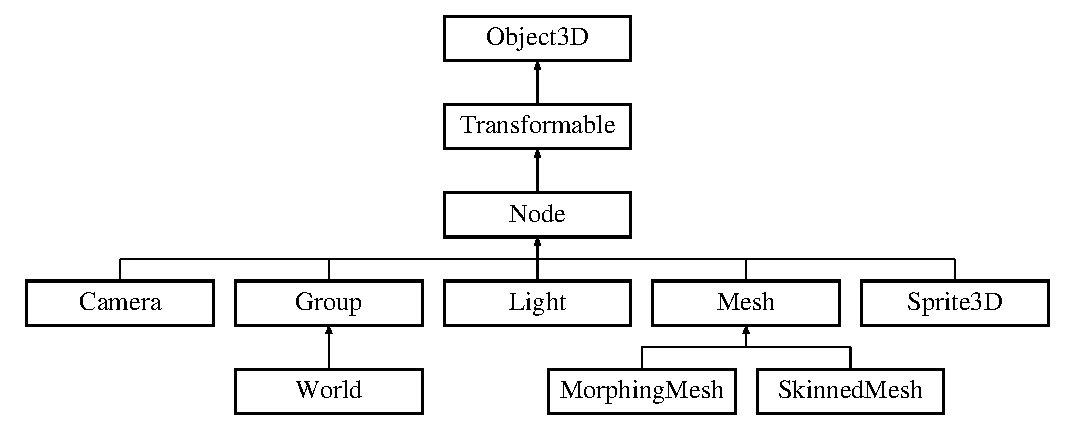
\includegraphics[height=5cm]{classm3g_1_1Node}
\end{center}
\end{figure}
\subsection*{Classes}
\begin{CompactItemize}
\item 
struct \textbf{Alignment}
\end{CompactItemize}
\subsection*{Public Member Functions}
\begin{CompactItemize}
\item 
\hyperlink{classm3g_1_1Node_0d313fac56abd7ebe58a17f1530b879e}{Node} ()
\item 
virtual \hyperlink{classm3g_1_1Node_6fa6bf60f34f1e3efb0e59333428c9c8}{$\sim$Node} ()
\item 
void \hyperlink{classm3g_1_1Node_3db1b4be060fe3d4f3dbf9720ef85234}{align} (\hyperlink{classm3g_1_1Node}{Node} $\ast$reference)
\item 
virtual void \hyperlink{classm3g_1_1Node_415c0b110f95410ded9b85e5d99a496b}{addAnimationTrack} (\hyperlink{classm3g_1_1AnimationTrack}{AnimationTrack} $\ast$animation\_\-track)
\item 
virtual int \hyperlink{classm3g_1_1Node_8aad1ceab4c2a03609c8a42324ce484d}{animate} (int world\_\-time)
\item 
\hyperlink{classm3g_1_1Node}{Node} $\ast$ \hyperlink{classm3g_1_1Node_ca338390bd2dee287fe6f5cbc4e094e1}{getAlignmentReference} (int axis) const 
\item 
int \hyperlink{classm3g_1_1Node_e5bbf42b3d88193fda0b476e1b1da009}{getAlignmentTarget} (int axis) const 
\item 
float \hyperlink{classm3g_1_1Node_bf7e8f9d9f530274aaf27e69910f8689}{getAlphaFactor} () const 
\item 
\hyperlink{classm3g_1_1Node}{Node} $\ast$ \hyperlink{classm3g_1_1Node_ce26c2757f265bc6038e6818d2eb6ad9}{getParent} () const 
\item 
int \hyperlink{classm3g_1_1Node_a3c291c19cf805338fa4ad3c3deb663a}{getScope} () const 
\item 
bool \hyperlink{classm3g_1_1Node_206a2e95eb7db42e6880414f77858113}{getTransformTo} (\hyperlink{classm3g_1_1Node}{Node} $\ast$target, \hyperlink{classm3g_1_1Transform}{Transform} $\ast$transform) const 
\item 
bool \hyperlink{classm3g_1_1Node_b3187e5056afa4a94af03e34125c86b1}{isPickingEnabled} () const 
\item 
bool \hyperlink{classm3g_1_1Node_95020b155afed9552cc55377b09b1e86}{isRenderingEnabled} () const 
\item 
void \hyperlink{classm3g_1_1Node_dd1627aba90e63c166ecd3d7463d735a}{setAlignment} (\hyperlink{classm3g_1_1Node}{Node} $\ast$z\_\-ref, int z\_\-target, \hyperlink{classm3g_1_1Node}{Node} $\ast$y\_\-ref, int y\_\-target)
\item 
void \hyperlink{classm3g_1_1Node_b33c321ce240770e5eb64d0e20ea61cc}{setAlphaFactor} (float alpha\_\-factor)
\item 
void \hyperlink{classm3g_1_1Node_4f9296202713ac56ccae72d5e0c21d96}{setPickingEnable} (bool enable)
\item 
void \hyperlink{classm3g_1_1Node_58981ef7aea1bf0e630bcc065b2987e9}{setRenderingEnable} (bool enable)
\item 
void \hyperlink{classm3g_1_1Node_55f324f307a01705b9094a73af4ecd68}{setScope} (int scope)
\item 
virtual std::ostream \& \hyperlink{classm3g_1_1Node_6fea17fa1532df3794f8cb39cb4f911f}{print} (std::ostream \&out) const 
\end{CompactItemize}
\subsection*{Static Public Attributes}
\begin{CompactItemize}
\item 
static const int \hyperlink{classm3g_1_1Node_7b20f1b443e093d5ec5e990e73b47232}{NONE} = 144
\item 
static const int \hyperlink{classm3g_1_1Node_1b0d56eb173868ff472a6fd296c5bb6c}{ORIGIN} = 145
\item 
static const int \hyperlink{classm3g_1_1Node_dd4bccb7b9c652e726d58b06bd28dab2}{X\_\-AXIS} = 146
\item 
static const int \hyperlink{classm3g_1_1Node_3248ff73b5411ab0a66a38c451c8b6fe}{Y\_\-AXIS} = 147
\item 
static const int \hyperlink{classm3g_1_1Node_a928e648c9ae9b4706937831f77f0c67}{Z\_\-AXIS} = 148
\end{CompactItemize}
\subsection*{Protected Member Functions}
\begin{CompactItemize}
\item 
void \hyperlink{classm3g_1_1Node_880ecc7c1c091f7607eeae12ed100a9a}{setParent} (\hyperlink{classm3g_1_1Node}{Node} $\ast$node)
\item 
virtual void \hyperlink{classm3g_1_1Node_1efcb1973989d9963d5bd6d03065d389}{render} (int pass, int index=0) const 
\end{CompactItemize}
\subsection*{Friends}
\begin{CompactItemize}
\item 
\hypertarget{classm3g_1_1Node_2697825715974a353728f0d4d5658112}{
class \textbf{Group}}
\label{classm3g_1_1Node_2697825715974a353728f0d4d5658112}

\item 
\hypertarget{classm3g_1_1Node_7b4bcdf992c21ae83363f25df05b1d25}{
class \textbf{World}}
\label{classm3g_1_1Node_7b4bcdf992c21ae83363f25df05b1d25}

\item 
\hypertarget{classm3g_1_1Node_8174d4c629550c1ee279571250236ef4}{
class \textbf{Graphics3D}}
\label{classm3g_1_1Node_8174d4c629550c1ee279571250236ef4}

\item 
\hypertarget{classm3g_1_1Node_a41a130f156b145bffb3f4b5172c4c93}{
class \textbf{Mesh}}
\label{classm3g_1_1Node_a41a130f156b145bffb3f4b5172c4c93}

\end{CompactItemize}


\subsection{Detailed Description}
An abstract base class for all scene graph nodes. 

\subsection{Constructor \& Destructor Documentation}
\hypertarget{classm3g_1_1Node_0d313fac56abd7ebe58a17f1530b879e}{
\index{m3g::Node@{m3g::Node}!Node@{Node}}
\index{Node@{Node}!m3g::Node@{m3g::Node}}
\subsubsection[{Node}]{\setlength{\rightskip}{0pt plus 5cm}{\bf Node} ()}}
\label{classm3g_1_1Node_0d313fac56abd7ebe58a17f1530b879e}


Construct a new \hyperlink{classm3g_1_1Node}{Node} object. \hypertarget{classm3g_1_1Node_6fa6bf60f34f1e3efb0e59333428c9c8}{
\index{m3g::Node@{m3g::Node}!$\sim$Node@{$\sim$Node}}
\index{$\sim$Node@{$\sim$Node}!m3g::Node@{m3g::Node}}
\subsubsection[{$\sim$Node}]{\setlength{\rightskip}{0pt plus 5cm}$\sim${\bf Node} ()\hspace{0.3cm}{\tt  \mbox{[}virtual\mbox{]}}}}
\label{classm3g_1_1Node_6fa6bf60f34f1e3efb0e59333428c9c8}


Destruct this object. 

\subsection{Member Function Documentation}
\hypertarget{classm3g_1_1Node_415c0b110f95410ded9b85e5d99a496b}{
\index{m3g::Node@{m3g::Node}!addAnimationTrack@{addAnimationTrack}}
\index{addAnimationTrack@{addAnimationTrack}!m3g::Node@{m3g::Node}}
\subsubsection[{addAnimationTrack}]{\setlength{\rightskip}{0pt plus 5cm}void addAnimationTrack ({\bf AnimationTrack} $\ast$ {\em animation\_\-track})\hspace{0.3cm}{\tt  \mbox{[}virtual\mbox{]}}}}
\label{classm3g_1_1Node_415c0b110f95410ded9b85e5d99a496b}


Adds the given \hyperlink{classm3g_1_1AnimationTrack}{AnimationTrack} to this \hyperlink{classm3g_1_1Object3D}{Object3D}, potentially changing the order and indices of the previously added tracks. 

Reimplemented from \hyperlink{classm3g_1_1Transformable_415c0b110f95410ded9b85e5d99a496b}{Transformable}.

Reimplemented in \hyperlink{classm3g_1_1Camera_415c0b110f95410ded9b85e5d99a496b}{Camera}, \hyperlink{classm3g_1_1Light_415c0b110f95410ded9b85e5d99a496b}{Light}, \hyperlink{classm3g_1_1MorphingMesh_415c0b110f95410ded9b85e5d99a496b}{MorphingMesh}, and \hyperlink{classm3g_1_1Sprite3D_415c0b110f95410ded9b85e5d99a496b}{Sprite3D}.\hypertarget{classm3g_1_1Node_3db1b4be060fe3d4f3dbf9720ef85234}{
\index{m3g::Node@{m3g::Node}!align@{align}}
\index{align@{align}!m3g::Node@{m3g::Node}}
\subsubsection[{align}]{\setlength{\rightskip}{0pt plus 5cm}void align ({\bf Node} $\ast$ {\em reference})}}
\label{classm3g_1_1Node_3db1b4be060fe3d4f3dbf9720ef85234}


Applies alignments to this \hyperlink{classm3g_1_1Node}{Node} and its descendants. \hypertarget{classm3g_1_1Node_8aad1ceab4c2a03609c8a42324ce484d}{
\index{m3g::Node@{m3g::Node}!animate@{animate}}
\index{animate@{animate}!m3g::Node@{m3g::Node}}
\subsubsection[{animate}]{\setlength{\rightskip}{0pt plus 5cm}int animate (int {\em world\_\-time})\hspace{0.3cm}{\tt  \mbox{[}virtual\mbox{]}}}}
\label{classm3g_1_1Node_8aad1ceab4c2a03609c8a42324ce484d}


Updates all animated properties in this \hyperlink{classm3g_1_1Object3D}{Object3D} and all Object3Ds that are reachable from this \hyperlink{classm3g_1_1Object3D}{Object3D}. 

Reimplemented from \hyperlink{classm3g_1_1Transformable_8aad1ceab4c2a03609c8a42324ce484d}{Transformable}.

Reimplemented in \hyperlink{classm3g_1_1Camera_8aad1ceab4c2a03609c8a42324ce484d}{Camera}, \hyperlink{classm3g_1_1Light_8aad1ceab4c2a03609c8a42324ce484d}{Light}, \hyperlink{classm3g_1_1Mesh_82cfeb67ca66b93e2ca7bda9a4f0e2aa}{Mesh}, \hyperlink{classm3g_1_1MorphingMesh_8aad1ceab4c2a03609c8a42324ce484d}{MorphingMesh}, \hyperlink{classm3g_1_1Sprite3D_8aad1ceab4c2a03609c8a42324ce484d}{Sprite3D}, and \hyperlink{classm3g_1_1World_8aad1ceab4c2a03609c8a42324ce484d}{World}.\hypertarget{classm3g_1_1Node_ca338390bd2dee287fe6f5cbc4e094e1}{
\index{m3g::Node@{m3g::Node}!getAlignmentReference@{getAlignmentReference}}
\index{getAlignmentReference@{getAlignmentReference}!m3g::Node@{m3g::Node}}
\subsubsection[{getAlignmentReference}]{\setlength{\rightskip}{0pt plus 5cm}{\bf Node} $\ast$ getAlignmentReference (int {\em axis}) const}}
\label{classm3g_1_1Node_ca338390bd2dee287fe6f5cbc4e094e1}


Returns the alignment reference node for the given axis. \hypertarget{classm3g_1_1Node_e5bbf42b3d88193fda0b476e1b1da009}{
\index{m3g::Node@{m3g::Node}!getAlignmentTarget@{getAlignmentTarget}}
\index{getAlignmentTarget@{getAlignmentTarget}!m3g::Node@{m3g::Node}}
\subsubsection[{getAlignmentTarget}]{\setlength{\rightskip}{0pt plus 5cm}int getAlignmentTarget (int {\em axis}) const}}
\label{classm3g_1_1Node_e5bbf42b3d88193fda0b476e1b1da009}


Returns tthe alignment target for the given axis. \hypertarget{classm3g_1_1Node_bf7e8f9d9f530274aaf27e69910f8689}{
\index{m3g::Node@{m3g::Node}!getAlphaFactor@{getAlphaFactor}}
\index{getAlphaFactor@{getAlphaFactor}!m3g::Node@{m3g::Node}}
\subsubsection[{getAlphaFactor}]{\setlength{\rightskip}{0pt plus 5cm}float getAlphaFactor () const}}
\label{classm3g_1_1Node_bf7e8f9d9f530274aaf27e69910f8689}


Retrieves the alpha factor of this \hyperlink{classm3g_1_1Node}{Node}. \hypertarget{classm3g_1_1Node_ce26c2757f265bc6038e6818d2eb6ad9}{
\index{m3g::Node@{m3g::Node}!getParent@{getParent}}
\index{getParent@{getParent}!m3g::Node@{m3g::Node}}
\subsubsection[{getParent}]{\setlength{\rightskip}{0pt plus 5cm}{\bf Node} $\ast$ getParent () const}}
\label{classm3g_1_1Node_ce26c2757f265bc6038e6818d2eb6ad9}


Returns the scene graph parent of this node. \hypertarget{classm3g_1_1Node_a3c291c19cf805338fa4ad3c3deb663a}{
\index{m3g::Node@{m3g::Node}!getScope@{getScope}}
\index{getScope@{getScope}!m3g::Node@{m3g::Node}}
\subsubsection[{getScope}]{\setlength{\rightskip}{0pt plus 5cm}int getScope () const}}
\label{classm3g_1_1Node_a3c291c19cf805338fa4ad3c3deb663a}


Retrieves the scope of this \hyperlink{classm3g_1_1Node}{Node}. \hypertarget{classm3g_1_1Node_206a2e95eb7db42e6880414f77858113}{
\index{m3g::Node@{m3g::Node}!getTransformTo@{getTransformTo}}
\index{getTransformTo@{getTransformTo}!m3g::Node@{m3g::Node}}
\subsubsection[{getTransformTo}]{\setlength{\rightskip}{0pt plus 5cm}bool getTransformTo ({\bf Node} $\ast$ {\em target}, \/  {\bf Transform} $\ast$ {\em transform}) const}}
\label{classm3g_1_1Node_206a2e95eb7db42e6880414f77858113}


Gets the composite transfformation from this node to the given node. \hypertarget{classm3g_1_1Node_b3187e5056afa4a94af03e34125c86b1}{
\index{m3g::Node@{m3g::Node}!isPickingEnabled@{isPickingEnabled}}
\index{isPickingEnabled@{isPickingEnabled}!m3g::Node@{m3g::Node}}
\subsubsection[{isPickingEnabled}]{\setlength{\rightskip}{0pt plus 5cm}bool isPickingEnabled () const}}
\label{classm3g_1_1Node_b3187e5056afa4a94af03e34125c86b1}


Retrieves the picking enable flag of this \hyperlink{classm3g_1_1Node}{Node}. \hypertarget{classm3g_1_1Node_95020b155afed9552cc55377b09b1e86}{
\index{m3g::Node@{m3g::Node}!isRenderingEnabled@{isRenderingEnabled}}
\index{isRenderingEnabled@{isRenderingEnabled}!m3g::Node@{m3g::Node}}
\subsubsection[{isRenderingEnabled}]{\setlength{\rightskip}{0pt plus 5cm}bool isRenderingEnabled () const}}
\label{classm3g_1_1Node_95020b155afed9552cc55377b09b1e86}


Retrieves the rendering neble flag of this \hyperlink{classm3g_1_1Node}{Node}. \hypertarget{classm3g_1_1Node_6fea17fa1532df3794f8cb39cb4f911f}{
\index{m3g::Node@{m3g::Node}!print@{print}}
\index{print@{print}!m3g::Node@{m3g::Node}}
\subsubsection[{print}]{\setlength{\rightskip}{0pt plus 5cm}std::ostream \& print (std::ostream \& {\em out}) const\hspace{0.3cm}{\tt  \mbox{[}virtual\mbox{]}}}}
\label{classm3g_1_1Node_6fea17fa1532df3794f8cb39cb4f911f}


Print out information of this object. 

Reimplemented from \hyperlink{classm3g_1_1Transformable_6fea17fa1532df3794f8cb39cb4f911f}{Transformable}.

Reimplemented in \hyperlink{classm3g_1_1Camera_6fea17fa1532df3794f8cb39cb4f911f}{Camera}, \hyperlink{classm3g_1_1Light_6fea17fa1532df3794f8cb39cb4f911f}{Light}, \hyperlink{classm3g_1_1Mesh_6fea17fa1532df3794f8cb39cb4f911f}{Mesh}, \hyperlink{classm3g_1_1MorphingMesh_6fea17fa1532df3794f8cb39cb4f911f}{MorphingMesh}, \hyperlink{classm3g_1_1SkinnedMesh_6fea17fa1532df3794f8cb39cb4f911f}{SkinnedMesh}, \hyperlink{classm3g_1_1Sprite3D_6fea17fa1532df3794f8cb39cb4f911f}{Sprite3D}, and \hyperlink{classm3g_1_1World_6fea17fa1532df3794f8cb39cb4f911f}{World}.\hypertarget{classm3g_1_1Node_1efcb1973989d9963d5bd6d03065d389}{
\index{m3g::Node@{m3g::Node}!render@{render}}
\index{render@{render}!m3g::Node@{m3g::Node}}
\subsubsection[{render}]{\setlength{\rightskip}{0pt plus 5cm}void render (int {\em pass}, \/  int {\em index} = {\tt 0}) const\hspace{0.3cm}{\tt  \mbox{[}protected, virtual\mbox{]}}}}
\label{classm3g_1_1Node_1efcb1973989d9963d5bd6d03065d389}


Note: \hyperlink{classm3g_1_1Node}{Node} should be rendered via all rendering pass. 

Reimplemented from \hyperlink{classm3g_1_1Transformable_1efcb1973989d9963d5bd6d03065d389}{Transformable}.

Reimplemented in \hyperlink{classm3g_1_1Camera_1efcb1973989d9963d5bd6d03065d389}{Camera}, \hyperlink{classm3g_1_1Mesh_1efcb1973989d9963d5bd6d03065d389}{Mesh}, \hyperlink{classm3g_1_1MorphingMesh_1efcb1973989d9963d5bd6d03065d389}{MorphingMesh}, \hyperlink{classm3g_1_1SkinnedMesh_1efcb1973989d9963d5bd6d03065d389}{SkinnedMesh}, \hyperlink{classm3g_1_1Sprite3D_1efcb1973989d9963d5bd6d03065d389}{Sprite3D}, and \hyperlink{classm3g_1_1World_1efcb1973989d9963d5bd6d03065d389}{World}.\hypertarget{classm3g_1_1Node_dd1627aba90e63c166ecd3d7463d735a}{
\index{m3g::Node@{m3g::Node}!setAlignment@{setAlignment}}
\index{setAlignment@{setAlignment}!m3g::Node@{m3g::Node}}
\subsubsection[{setAlignment}]{\setlength{\rightskip}{0pt plus 5cm}void setAlignment ({\bf Node} $\ast$ {\em z\_\-ref}, \/  int {\em z\_\-target}, \/  {\bf Node} $\ast$ {\em y\_\-ref}, \/  int {\em y\_\-target})}}
\label{classm3g_1_1Node_dd1627aba90e63c166ecd3d7463d735a}


Sts this node to align with the given other nodes(s), or disables alignment. \hypertarget{classm3g_1_1Node_b33c321ce240770e5eb64d0e20ea61cc}{
\index{m3g::Node@{m3g::Node}!setAlphaFactor@{setAlphaFactor}}
\index{setAlphaFactor@{setAlphaFactor}!m3g::Node@{m3g::Node}}
\subsubsection[{setAlphaFactor}]{\setlength{\rightskip}{0pt plus 5cm}void setAlphaFactor (float {\em alpha\_\-factor})}}
\label{classm3g_1_1Node_b33c321ce240770e5eb64d0e20ea61cc}


Sets the alpha factor for this \hyperlink{classm3g_1_1Node}{Node}. \hypertarget{classm3g_1_1Node_880ecc7c1c091f7607eeae12ed100a9a}{
\index{m3g::Node@{m3g::Node}!setParent@{setParent}}
\index{setParent@{setParent}!m3g::Node@{m3g::Node}}
\subsubsection[{setParent}]{\setlength{\rightskip}{0pt plus 5cm}void setParent ({\bf Node} $\ast$ {\em node})\hspace{0.3cm}{\tt  \mbox{[}protected\mbox{]}}}}
\label{classm3g_1_1Node_880ecc7c1c091f7607eeae12ed100a9a}


Sets parent of this node. \hypertarget{classm3g_1_1Node_4f9296202713ac56ccae72d5e0c21d96}{
\index{m3g::Node@{m3g::Node}!setPickingEnable@{setPickingEnable}}
\index{setPickingEnable@{setPickingEnable}!m3g::Node@{m3g::Node}}
\subsubsection[{setPickingEnable}]{\setlength{\rightskip}{0pt plus 5cm}void setPickingEnable (bool {\em enable})}}
\label{classm3g_1_1Node_4f9296202713ac56ccae72d5e0c21d96}


Sets the picking enable flag of this \hyperlink{classm3g_1_1Node}{Node}. \hypertarget{classm3g_1_1Node_58981ef7aea1bf0e630bcc065b2987e9}{
\index{m3g::Node@{m3g::Node}!setRenderingEnable@{setRenderingEnable}}
\index{setRenderingEnable@{setRenderingEnable}!m3g::Node@{m3g::Node}}
\subsubsection[{setRenderingEnable}]{\setlength{\rightskip}{0pt plus 5cm}void setRenderingEnable (bool {\em enable})}}
\label{classm3g_1_1Node_58981ef7aea1bf0e630bcc065b2987e9}


Sets the rendering enable flag of this \hyperlink{classm3g_1_1Node}{Node}. \hypertarget{classm3g_1_1Node_55f324f307a01705b9094a73af4ecd68}{
\index{m3g::Node@{m3g::Node}!setScope@{setScope}}
\index{setScope@{setScope}!m3g::Node@{m3g::Node}}
\subsubsection[{setScope}]{\setlength{\rightskip}{0pt plus 5cm}void setScope (int {\em scope})}}
\label{classm3g_1_1Node_55f324f307a01705b9094a73af4ecd68}


Sets the scope of this node. 

\subsection{Member Data Documentation}
\hypertarget{classm3g_1_1Node_7b20f1b443e093d5ec5e990e73b47232}{
\index{m3g::Node@{m3g::Node}!NONE@{NONE}}
\index{NONE@{NONE}!m3g::Node@{m3g::Node}}
\subsubsection[{NONE}]{\setlength{\rightskip}{0pt plus 5cm}const int {\bf NONE} = 144\hspace{0.3cm}{\tt  \mbox{[}static\mbox{]}}}}
\label{classm3g_1_1Node_7b20f1b443e093d5ec5e990e73b47232}


Specifies for the setAlignment method that no alignment should be done for the specified axis. \hypertarget{classm3g_1_1Node_1b0d56eb173868ff472a6fd296c5bb6c}{
\index{m3g::Node@{m3g::Node}!ORIGIN@{ORIGIN}}
\index{ORIGIN@{ORIGIN}!m3g::Node@{m3g::Node}}
\subsubsection[{ORIGIN}]{\setlength{\rightskip}{0pt plus 5cm}const int {\bf ORIGIN} = 145\hspace{0.3cm}{\tt  \mbox{[}static\mbox{]}}}}
\label{classm3g_1_1Node_1b0d56eb173868ff472a6fd296c5bb6c}


Specifies the origin of the reference node as an orientation reference for the setAlighnment method. \hypertarget{classm3g_1_1Node_dd4bccb7b9c652e726d58b06bd28dab2}{
\index{m3g::Node@{m3g::Node}!X\_\-AXIS@{X\_\-AXIS}}
\index{X\_\-AXIS@{X\_\-AXIS}!m3g::Node@{m3g::Node}}
\subsubsection[{X\_\-AXIS}]{\setlength{\rightskip}{0pt plus 5cm}const int {\bf X\_\-AXIS} = 146\hspace{0.3cm}{\tt  \mbox{[}static\mbox{]}}}}
\label{classm3g_1_1Node_dd4bccb7b9c652e726d58b06bd28dab2}


Specifies the X axis of the reference node as an orientation reference for the setAlignement method. \hypertarget{classm3g_1_1Node_3248ff73b5411ab0a66a38c451c8b6fe}{
\index{m3g::Node@{m3g::Node}!Y\_\-AXIS@{Y\_\-AXIS}}
\index{Y\_\-AXIS@{Y\_\-AXIS}!m3g::Node@{m3g::Node}}
\subsubsection[{Y\_\-AXIS}]{\setlength{\rightskip}{0pt plus 5cm}const int {\bf Y\_\-AXIS} = 147\hspace{0.3cm}{\tt  \mbox{[}static\mbox{]}}}}
\label{classm3g_1_1Node_3248ff73b5411ab0a66a38c451c8b6fe}


Specifieds the Y axis of the reference node as an orientation reference for the setAlignment mehotd. \hypertarget{classm3g_1_1Node_a928e648c9ae9b4706937831f77f0c67}{
\index{m3g::Node@{m3g::Node}!Z\_\-AXIS@{Z\_\-AXIS}}
\index{Z\_\-AXIS@{Z\_\-AXIS}!m3g::Node@{m3g::Node}}
\subsubsection[{Z\_\-AXIS}]{\setlength{\rightskip}{0pt plus 5cm}const int {\bf Z\_\-AXIS} = 148\hspace{0.3cm}{\tt  \mbox{[}static\mbox{]}}}}
\label{classm3g_1_1Node_a928e648c9ae9b4706937831f77f0c67}


Specifieds the Z axis of the reference node as an orientation reference for the setAlignment mehotd. 

The documentation for this class was generated from the following files:\begin{CompactItemize}
\item 
/work/desktop-m3g/src/Node.hpp\item 
/work/desktop-m3g/src/Node.cpp\end{CompactItemize}

\hypertarget{classm3g_1_1Object3D}{
\section{Object3D Class Reference}
\label{classm3g_1_1Object3D}\index{m3g::Object3D@{m3g::Object3D}}
}
{\tt \#include $<$Object3D.hpp$>$}

Inheritance diagram for Object3D::\begin{figure}[H]
\begin{center}
\leavevmode
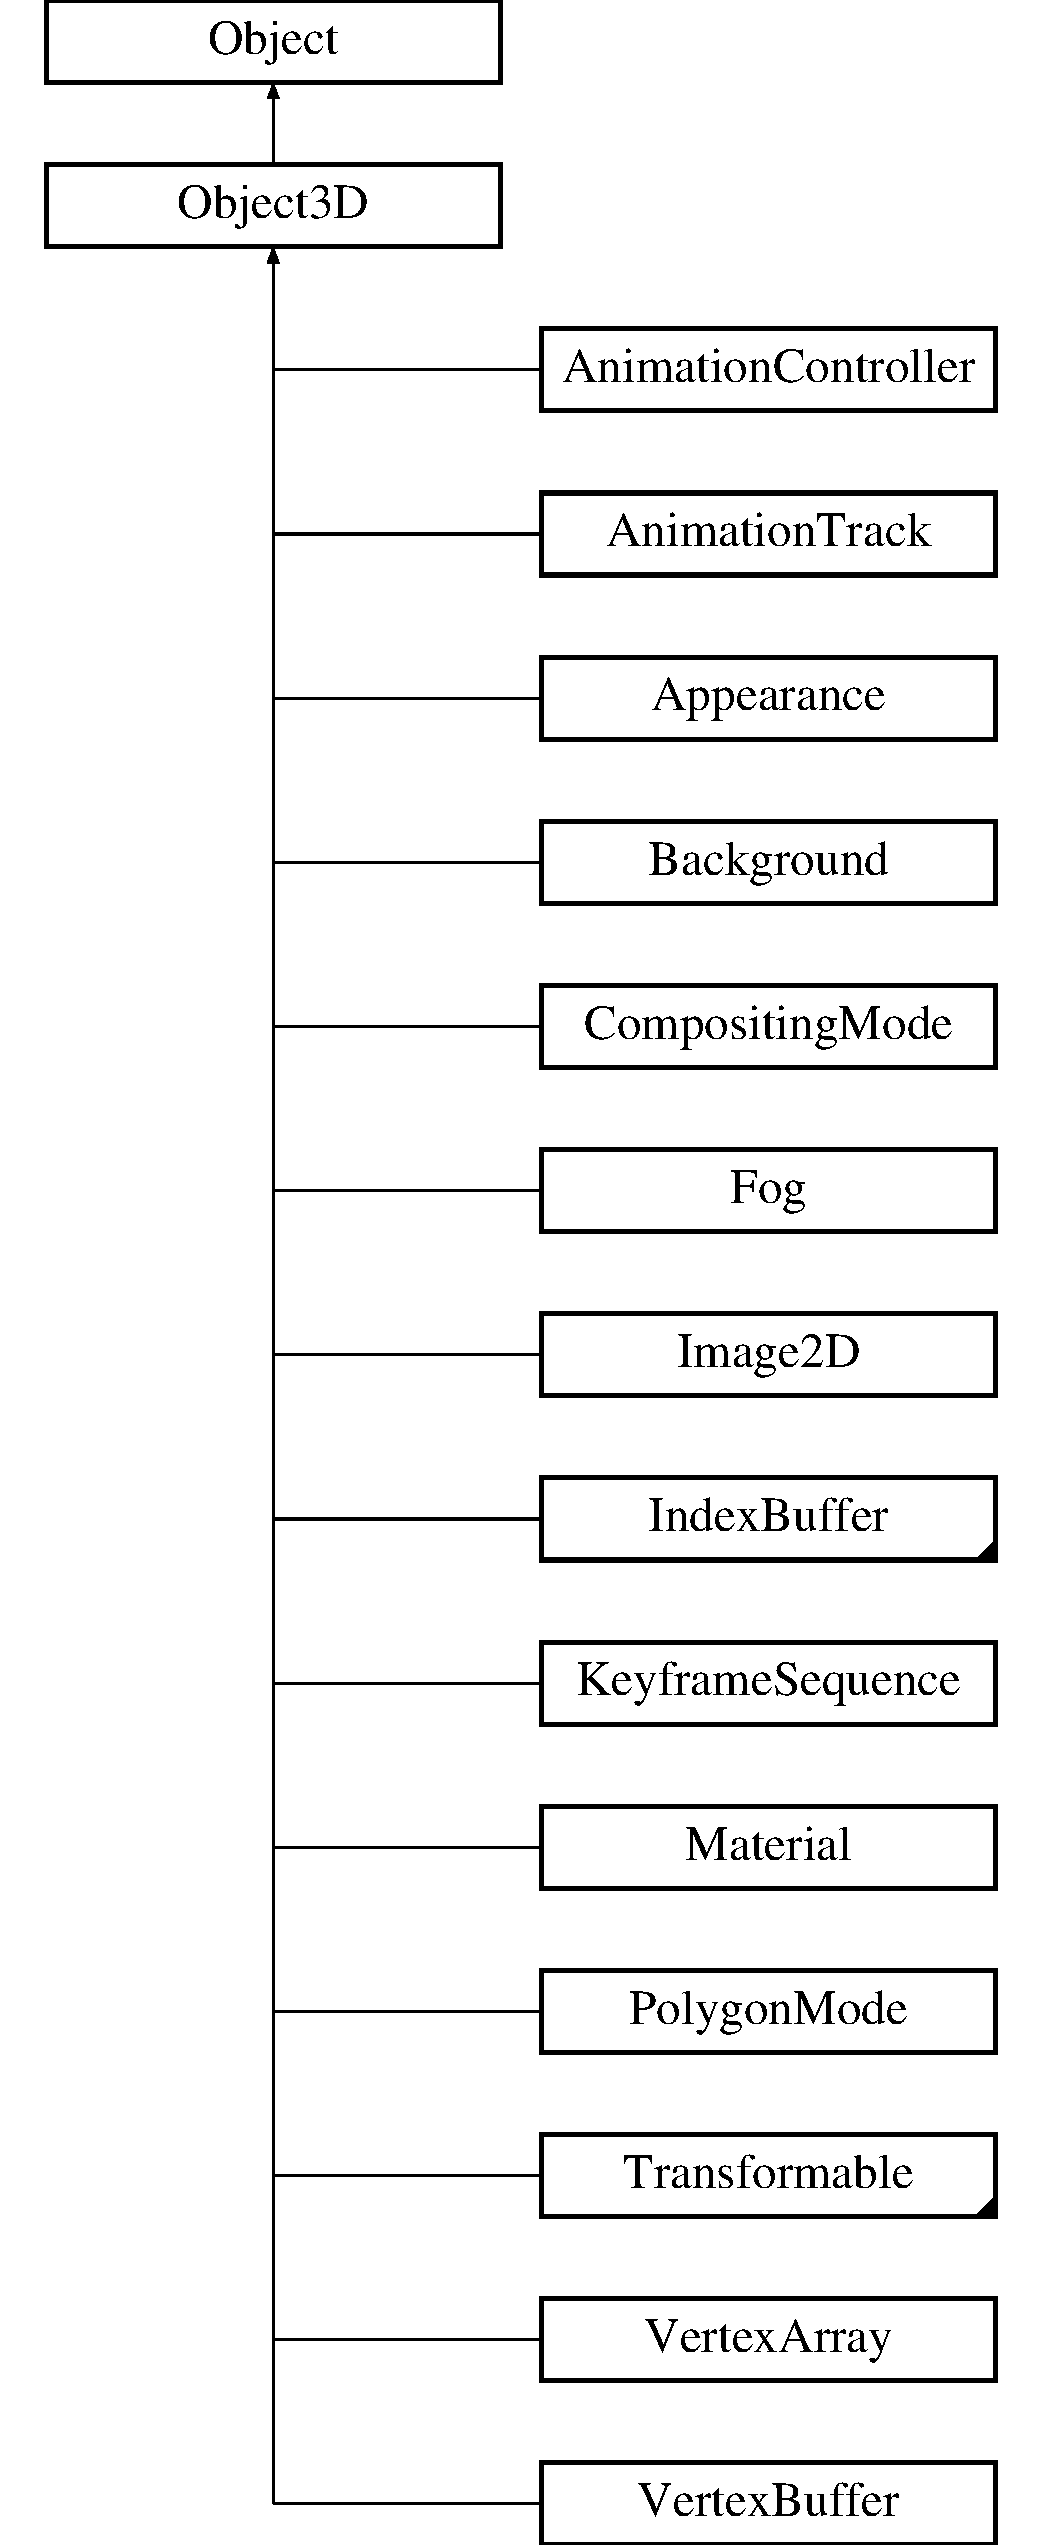
\includegraphics[height=12cm]{classm3g_1_1Object3D}
\end{center}
\end{figure}
\subsection*{Public Member Functions}
\begin{CompactItemize}
\item 
\hyperlink{classm3g_1_1Object3D_f4b10c33b9014a3f0a675ef4b699b773}{Object3D} ()
\item 
virtual \hyperlink{classm3g_1_1Object3D_8ece10725587e63a2c75283c16cc4df5}{$\sim$Object3D} ()
\item 
virtual int \hyperlink{classm3g_1_1Object3D_8aad1ceab4c2a03609c8a42324ce484d}{animate} (int world\_\-time)
\item 
virtual \hyperlink{classm3g_1_1Object3D}{Object3D} $\ast$ \hyperlink{classm3g_1_1Object3D_a25110dac934f867b83b73ad4741a0f4}{duplicate} () const 
\item 
virtual \hyperlink{classm3g_1_1Object3D}{Object3D} $\ast$ \hyperlink{classm3g_1_1Object3D_aa62f6aaac2e9359875f027ca05788ac}{find} (int userID) const 
\item 
\hyperlink{classm3g_1_1AnimationTrack}{AnimationTrack} $\ast$ \hyperlink{classm3g_1_1Object3D_f0978f3f2efe3227ca613da3361424dd}{getAnimationTrack} (int index) const 
\item 
int \hyperlink{classm3g_1_1Object3D_0926843b66090795972850376b8e4e6c}{getAnimationTrackCount} () const 
\item 
virtual int \hyperlink{classm3g_1_1Object3D_ddf91fbaaa866aa7aad5d530a69feba8}{getReferences} (\hyperlink{classm3g_1_1Object3D}{Object3D} $\ast$$\ast$references, int size) const 
\item 
int \hyperlink{classm3g_1_1Object3D_b8d9067364251d0208fcdc502d394e2c}{getUserID} () const 
\item 
void $\ast$ \hyperlink{classm3g_1_1Object3D_a9b8541216c1fa7792617218a5fb6672}{getUserObject} () const 
\item 
void \hyperlink{classm3g_1_1Object3D_e36d8f8544daee6bd4e2ccd6755ed03d}{removeAnimationTrack} (\hyperlink{classm3g_1_1AnimationTrack}{AnimationTrack} $\ast$animation\_\-track)
\item 
void \hyperlink{classm3g_1_1Object3D_5e4753e91dca5aa56abacb7fde69f332}{setUserID} (int userID)
\item 
void \hyperlink{classm3g_1_1Object3D_052563fbd888204955f1a56628882f14}{setUserObject} (void $\ast$user\_\-object\_\-value)
\item 
virtual std::ostream \& \hyperlink{classm3g_1_1Object3D_6fea17fa1532df3794f8cb39cb4f911f}{print} (std::ostream \&out) const 
\end{CompactItemize}
\subsection*{Public Attributes}
\begin{CompactItemize}
\item 
\hypertarget{classm3g_1_1Object3D_11d260eb623ff241a55524ad8bc9beb4}{
PROTECTED \textbf{\_\-\_\-pad0\_\-\_\-}: virtual void addAnimationTrack (\hyperlink{classm3g_1_1AnimationTrack}{AnimationTrack}$\ast$ animation\_\-track)}
\label{classm3g_1_1Object3D_11d260eb623ff241a55524ad8bc9beb4}

\end{CompactItemize}
\subsection*{Protected Member Functions}
\begin{CompactItemize}
\item 
virtual void \hyperlink{classm3g_1_1Object3D_1efcb1973989d9963d5bd6d03065d389}{render} (int pass, int index=0) const 
\item 
int \hyperlink{classm3g_1_1Object3D_06be1b37b707b5f227cba2308043f3df}{getObjectType} () const 
\item 
virtual void \hyperlink{classm3g_1_1Object3D_4dadb21b568b0230fac106f15040138c}{findByObjectType} (int obj\_\-type, std::vector$<$ \hyperlink{classm3g_1_1Object3D}{Object3D} $\ast$ $>$ \&objs) const 
\end{CompactItemize}
\subsection*{Protected Attributes}
\begin{CompactItemize}
\item 
\hypertarget{classm3g_1_1Object3D_1868c0b310409e4b2258f29504e43760}{
PROTECTED \textbf{\_\-\_\-pad1\_\-\_\-}: void setObjectType (int type)}
\label{classm3g_1_1Object3D_1868c0b310409e4b2258f29504e43760}

\end{CompactItemize}


\subsection{Detailed Description}
An abstract base class for all objects that can be part of a 3D world. 

\subsection{Constructor \& Destructor Documentation}
\hypertarget{classm3g_1_1Object3D_f4b10c33b9014a3f0a675ef4b699b773}{
\index{m3g::Object3D@{m3g::Object3D}!Object3D@{Object3D}}
\index{Object3D@{Object3D}!m3g::Object3D@{m3g::Object3D}}
\subsubsection[{Object3D}]{\setlength{\rightskip}{0pt plus 5cm}{\bf Object3D} ()}}
\label{classm3g_1_1Object3D_f4b10c33b9014a3f0a675ef4b699b773}


Construct a new Objec3D object. \hypertarget{classm3g_1_1Object3D_8ece10725587e63a2c75283c16cc4df5}{
\index{m3g::Object3D@{m3g::Object3D}!$\sim$Object3D@{$\sim$Object3D}}
\index{$\sim$Object3D@{$\sim$Object3D}!m3g::Object3D@{m3g::Object3D}}
\subsubsection[{$\sim$Object3D}]{\setlength{\rightskip}{0pt plus 5cm}$\sim${\bf Object3D} ()\hspace{0.3cm}{\tt  \mbox{[}virtual\mbox{]}}}}
\label{classm3g_1_1Object3D_8ece10725587e63a2c75283c16cc4df5}


Destruct this object. 

\subsection{Member Function Documentation}
\hypertarget{classm3g_1_1Object3D_8aad1ceab4c2a03609c8a42324ce484d}{
\index{m3g::Object3D@{m3g::Object3D}!animate@{animate}}
\index{animate@{animate}!m3g::Object3D@{m3g::Object3D}}
\subsubsection[{animate}]{\setlength{\rightskip}{0pt plus 5cm}int animate (int {\em world\_\-time})\hspace{0.3cm}{\tt  \mbox{[}virtual\mbox{]}}}}
\label{classm3g_1_1Object3D_8aad1ceab4c2a03609c8a42324ce484d}


Updates all animated properties in this \hyperlink{classm3g_1_1Object3D}{Object3D} and all Object3Ds that are reachable from this \hyperlink{classm3g_1_1Object3D}{Object3D}. 

Reimplemented in \hyperlink{classm3g_1_1Appearance_8aad1ceab4c2a03609c8a42324ce484d}{Appearance}, \hyperlink{classm3g_1_1Background_8aad1ceab4c2a03609c8a42324ce484d}{Background}, \hyperlink{classm3g_1_1Camera_8aad1ceab4c2a03609c8a42324ce484d}{Camera}, \hyperlink{classm3g_1_1Fog_8aad1ceab4c2a03609c8a42324ce484d}{Fog}, \hyperlink{classm3g_1_1Material_8aad1ceab4c2a03609c8a42324ce484d}{Material}, \hyperlink{classm3g_1_1Mesh_82cfeb67ca66b93e2ca7bda9a4f0e2aa}{Mesh}, \hyperlink{classm3g_1_1MorphingMesh_8aad1ceab4c2a03609c8a42324ce484d}{MorphingMesh}, \hyperlink{classm3g_1_1Node_8aad1ceab4c2a03609c8a42324ce484d}{Node}, \hyperlink{classm3g_1_1Texture2D_82cfeb67ca66b93e2ca7bda9a4f0e2aa}{Texture2D}, \hyperlink{classm3g_1_1Transformable_8aad1ceab4c2a03609c8a42324ce484d}{Transformable}, \hyperlink{classm3g_1_1VertexBuffer_82cfeb67ca66b93e2ca7bda9a4f0e2aa}{VertexBuffer}, and \hyperlink{classm3g_1_1World_8aad1ceab4c2a03609c8a42324ce484d}{World}.\hypertarget{classm3g_1_1Object3D_a25110dac934f867b83b73ad4741a0f4}{
\index{m3g::Object3D@{m3g::Object3D}!duplicate@{duplicate}}
\index{duplicate@{duplicate}!m3g::Object3D@{m3g::Object3D}}
\subsubsection[{duplicate}]{\setlength{\rightskip}{0pt plus 5cm}{\bf Object3D} $\ast$ duplicate () const\hspace{0.3cm}{\tt  \mbox{[}virtual\mbox{]}}}}
\label{classm3g_1_1Object3D_a25110dac934f867b83b73ad4741a0f4}


Creates a duplicate of this \hyperlink{classm3g_1_1Object3D}{Object3D}. \hypertarget{classm3g_1_1Object3D_aa62f6aaac2e9359875f027ca05788ac}{
\index{m3g::Object3D@{m3g::Object3D}!find@{find}}
\index{find@{find}!m3g::Object3D@{m3g::Object3D}}
\subsubsection[{find}]{\setlength{\rightskip}{0pt plus 5cm}{\bf Object3D} $\ast$ find (int {\em userID}) const\hspace{0.3cm}{\tt  \mbox{[}virtual\mbox{]}}}}
\label{classm3g_1_1Object3D_aa62f6aaac2e9359875f027ca05788ac}


Retrieves an object that has the given uer ID and is reachable from this object. \hypertarget{classm3g_1_1Object3D_4dadb21b568b0230fac106f15040138c}{
\index{m3g::Object3D@{m3g::Object3D}!findByObjectType@{findByObjectType}}
\index{findByObjectType@{findByObjectType}!m3g::Object3D@{m3g::Object3D}}
\subsubsection[{findByObjectType}]{\setlength{\rightskip}{0pt plus 5cm}void findByObjectType (int {\em obj\_\-type}, \/  std::vector$<$ {\bf Object3D} $\ast$ $>$ \& {\em objs}) const\hspace{0.3cm}{\tt  \mbox{[}protected, virtual\mbox{]}}}}
\label{classm3g_1_1Object3D_4dadb21b568b0230fac106f15040138c}


Find all objects by object type. 

Reimplemented in \hyperlink{classm3g_1_1Appearance_4dadb21b568b0230fac106f15040138c}{Appearance}, \hyperlink{classm3g_1_1Texture2D_4dadb21b568b0230fac106f15040138c}{Texture2D}, and \hyperlink{classm3g_1_1VertexBuffer_4dadb21b568b0230fac106f15040138c}{VertexBuffer}.\hypertarget{classm3g_1_1Object3D_f0978f3f2efe3227ca613da3361424dd}{
\index{m3g::Object3D@{m3g::Object3D}!getAnimationTrack@{getAnimationTrack}}
\index{getAnimationTrack@{getAnimationTrack}!m3g::Object3D@{m3g::Object3D}}
\subsubsection[{getAnimationTrack}]{\setlength{\rightskip}{0pt plus 5cm}{\bf AnimationTrack} $\ast$ getAnimationTrack (int {\em index}) const}}
\label{classm3g_1_1Object3D_f0978f3f2efe3227ca613da3361424dd}


Gets an \hyperlink{classm3g_1_1AnimationTrack}{AnimationTrack} by index. \hypertarget{classm3g_1_1Object3D_0926843b66090795972850376b8e4e6c}{
\index{m3g::Object3D@{m3g::Object3D}!getAnimationTrackCount@{getAnimationTrackCount}}
\index{getAnimationTrackCount@{getAnimationTrackCount}!m3g::Object3D@{m3g::Object3D}}
\subsubsection[{getAnimationTrackCount}]{\setlength{\rightskip}{0pt plus 5cm}int getAnimationTrackCount () const}}
\label{classm3g_1_1Object3D_0926843b66090795972850376b8e4e6c}


Gets the number of AnimationTracks currently associated with this \hyperlink{classm3g_1_1Object3D}{Object3D}. \hypertarget{classm3g_1_1Object3D_06be1b37b707b5f227cba2308043f3df}{
\index{m3g::Object3D@{m3g::Object3D}!getObjectType@{getObjectType}}
\index{getObjectType@{getObjectType}!m3g::Object3D@{m3g::Object3D}}
\subsubsection[{getObjectType}]{\setlength{\rightskip}{0pt plus 5cm}int getObjectType () const\hspace{0.3cm}{\tt  \mbox{[}protected\mbox{]}}}}
\label{classm3g_1_1Object3D_06be1b37b707b5f227cba2308043f3df}


Retrievs object type. \hypertarget{classm3g_1_1Object3D_ddf91fbaaa866aa7aad5d530a69feba8}{
\index{m3g::Object3D@{m3g::Object3D}!getReferences@{getReferences}}
\index{getReferences@{getReferences}!m3g::Object3D@{m3g::Object3D}}
\subsubsection[{getReferences}]{\setlength{\rightskip}{0pt plus 5cm}int getReferences ({\bf Object3D} $\ast$$\ast$ {\em references}, \/  int {\em size}) const\hspace{0.3cm}{\tt  \mbox{[}virtual\mbox{]}}}}
\label{classm3g_1_1Object3D_ddf91fbaaa866aa7aad5d530a69feba8}


Returns the number of direct \hyperlink{classm3g_1_1Object3D}{Object3D} references in this object, and fills in the objects to the given array. \hypertarget{classm3g_1_1Object3D_b8d9067364251d0208fcdc502d394e2c}{
\index{m3g::Object3D@{m3g::Object3D}!getUserID@{getUserID}}
\index{getUserID@{getUserID}!m3g::Object3D@{m3g::Object3D}}
\subsubsection[{getUserID}]{\setlength{\rightskip}{0pt plus 5cm}int getUserID () const}}
\label{classm3g_1_1Object3D_b8d9067364251d0208fcdc502d394e2c}


Gets the user ID of this object. \hypertarget{classm3g_1_1Object3D_a9b8541216c1fa7792617218a5fb6672}{
\index{m3g::Object3D@{m3g::Object3D}!getUserObject@{getUserObject}}
\index{getUserObject@{getUserObject}!m3g::Object3D@{m3g::Object3D}}
\subsubsection[{getUserObject}]{\setlength{\rightskip}{0pt plus 5cm}void $\ast$ getUserObject () const}}
\label{classm3g_1_1Object3D_a9b8541216c1fa7792617218a5fb6672}


Rerieves the user object that is currently associated with this \hyperlink{classm3g_1_1Object3D}{Object3D}. \hypertarget{classm3g_1_1Object3D_6fea17fa1532df3794f8cb39cb4f911f}{
\index{m3g::Object3D@{m3g::Object3D}!print@{print}}
\index{print@{print}!m3g::Object3D@{m3g::Object3D}}
\subsubsection[{print}]{\setlength{\rightskip}{0pt plus 5cm}std::ostream \& print (std::ostream \& {\em out}) const\hspace{0.3cm}{\tt  \mbox{[}virtual\mbox{]}}}}
\label{classm3g_1_1Object3D_6fea17fa1532df3794f8cb39cb4f911f}


Print out information of this object, for debug only. 

Reimplemented in \hyperlink{classm3g_1_1AnimationController_6fea17fa1532df3794f8cb39cb4f911f}{AnimationController}, \hyperlink{classm3g_1_1AnimationTrack_6fea17fa1532df3794f8cb39cb4f911f}{AnimationTrack}, \hyperlink{classm3g_1_1Appearance_6fea17fa1532df3794f8cb39cb4f911f}{Appearance}, \hyperlink{classm3g_1_1Background_6fea17fa1532df3794f8cb39cb4f911f}{Background}, \hyperlink{classm3g_1_1Camera_6fea17fa1532df3794f8cb39cb4f911f}{Camera}, \hyperlink{classm3g_1_1CompositingMode_6fea17fa1532df3794f8cb39cb4f911f}{CompositingMode}, \hyperlink{classm3g_1_1Fog_6fea17fa1532df3794f8cb39cb4f911f}{Fog}, \hyperlink{classm3g_1_1Image2D_6fea17fa1532df3794f8cb39cb4f911f}{Image2D}, \hyperlink{classm3g_1_1IndexBuffer_6fea17fa1532df3794f8cb39cb4f911f}{IndexBuffer}, \hyperlink{classm3g_1_1KeyframeSequence_6fea17fa1532df3794f8cb39cb4f911f}{KeyframeSequence}, \hyperlink{classm3g_1_1Material_6fea17fa1532df3794f8cb39cb4f911f}{Material}, \hyperlink{classm3g_1_1Mesh_6fea17fa1532df3794f8cb39cb4f911f}{Mesh}, \hyperlink{classm3g_1_1MorphingMesh_6fea17fa1532df3794f8cb39cb4f911f}{MorphingMesh}, \hyperlink{classm3g_1_1Node_6fea17fa1532df3794f8cb39cb4f911f}{Node}, \hyperlink{classm3g_1_1SkinnedMesh_6fea17fa1532df3794f8cb39cb4f911f}{SkinnedMesh}, \hyperlink{classm3g_1_1Texture2D_6fea17fa1532df3794f8cb39cb4f911f}{Texture2D}, \hyperlink{classm3g_1_1Transformable_6fea17fa1532df3794f8cb39cb4f911f}{Transformable}, \hyperlink{classm3g_1_1TriangleStripArray_6fea17fa1532df3794f8cb39cb4f911f}{TriangleStripArray}, \hyperlink{classm3g_1_1VertexArray_6fea17fa1532df3794f8cb39cb4f911f}{VertexArray}, \hyperlink{classm3g_1_1VertexBuffer_6fea17fa1532df3794f8cb39cb4f911f}{VertexBuffer}, and \hyperlink{classm3g_1_1World_6fea17fa1532df3794f8cb39cb4f911f}{World}.\hypertarget{classm3g_1_1Object3D_e36d8f8544daee6bd4e2ccd6755ed03d}{
\index{m3g::Object3D@{m3g::Object3D}!removeAnimationTrack@{removeAnimationTrack}}
\index{removeAnimationTrack@{removeAnimationTrack}!m3g::Object3D@{m3g::Object3D}}
\subsubsection[{removeAnimationTrack}]{\setlength{\rightskip}{0pt plus 5cm}void removeAnimationTrack ({\bf AnimationTrack} $\ast$ {\em animation\_\-track})}}
\label{classm3g_1_1Object3D_e36d8f8544daee6bd4e2ccd6755ed03d}


Removves the given \hyperlink{classm3g_1_1AnimationTrack}{AnimationTrack} from this Objet3D, potentially changing the order and indices.of the remaining tracks. \hypertarget{classm3g_1_1Object3D_1efcb1973989d9963d5bd6d03065d389}{
\index{m3g::Object3D@{m3g::Object3D}!render@{render}}
\index{render@{render}!m3g::Object3D@{m3g::Object3D}}
\subsubsection[{render}]{\setlength{\rightskip}{0pt plus 5cm}void render (int {\em pass}, \/  int {\em index} = {\tt 0}) const\hspace{0.3cm}{\tt  \mbox{[}protected, virtual\mbox{]}}}}
\label{classm3g_1_1Object3D_1efcb1973989d9963d5bd6d03065d389}


Render this object, for inner use. 

Reimplemented in \hyperlink{classm3g_1_1Camera_1efcb1973989d9963d5bd6d03065d389}{Camera}, \hyperlink{classm3g_1_1CompositingMode_1efcb1973989d9963d5bd6d03065d389}{CompositingMode}, \hyperlink{classm3g_1_1Fog_1efcb1973989d9963d5bd6d03065d389}{Fog}, \hyperlink{classm3g_1_1IndexBuffer_1efcb1973989d9963d5bd6d03065d389}{IndexBuffer}, \hyperlink{classm3g_1_1Mesh_1efcb1973989d9963d5bd6d03065d389}{Mesh}, \hyperlink{classm3g_1_1MorphingMesh_1efcb1973989d9963d5bd6d03065d389}{MorphingMesh}, \hyperlink{classm3g_1_1Node_1efcb1973989d9963d5bd6d03065d389}{Node}, \hyperlink{classm3g_1_1SkinnedMesh_1efcb1973989d9963d5bd6d03065d389}{SkinnedMesh}, \hyperlink{classm3g_1_1Transformable_1efcb1973989d9963d5bd6d03065d389}{Transformable}, \hyperlink{classm3g_1_1TriangleStripArray_1efcb1973989d9963d5bd6d03065d389}{TriangleStripArray}, and \hyperlink{classm3g_1_1World_1efcb1973989d9963d5bd6d03065d389}{World}.\hypertarget{classm3g_1_1Object3D_5e4753e91dca5aa56abacb7fde69f332}{
\index{m3g::Object3D@{m3g::Object3D}!setUserID@{setUserID}}
\index{setUserID@{setUserID}!m3g::Object3D@{m3g::Object3D}}
\subsubsection[{setUserID}]{\setlength{\rightskip}{0pt plus 5cm}void setUserID (int {\em userID})}}
\label{classm3g_1_1Object3D_5e4753e91dca5aa56abacb7fde69f332}


Sets the user ID for this object. \hypertarget{classm3g_1_1Object3D_052563fbd888204955f1a56628882f14}{
\index{m3g::Object3D@{m3g::Object3D}!setUserObject@{setUserObject}}
\index{setUserObject@{setUserObject}!m3g::Object3D@{m3g::Object3D}}
\subsubsection[{setUserObject}]{\setlength{\rightskip}{0pt plus 5cm}void setUserObject (void $\ast$ {\em user\_\-object\_\-value})}}
\label{classm3g_1_1Object3D_052563fbd888204955f1a56628882f14}


Associates an arbitrary, application specific Object wth this \hyperlink{classm3g_1_1Object3D}{Object3D}. 

The documentation for this class was generated from the following files:\begin{CompactItemize}
\item 
/work/desktop-m3g/src/Object3D.hpp\item 
/work/desktop-m3g/src/Object3D.cpp\end{CompactItemize}

\hypertarget{classm3g_1_1PolygonMode}{
\section{クラス PolygonMode}
\label{classm3g_1_1PolygonMode}\index{m3g::PolygonMode@{m3g::PolygonMode}}
}
{\tt \#include $<$PolygonMode.hpp$>$}

PolygonModeに対する継承グラフ:\begin{figure}[H]
\begin{center}
\leavevmode
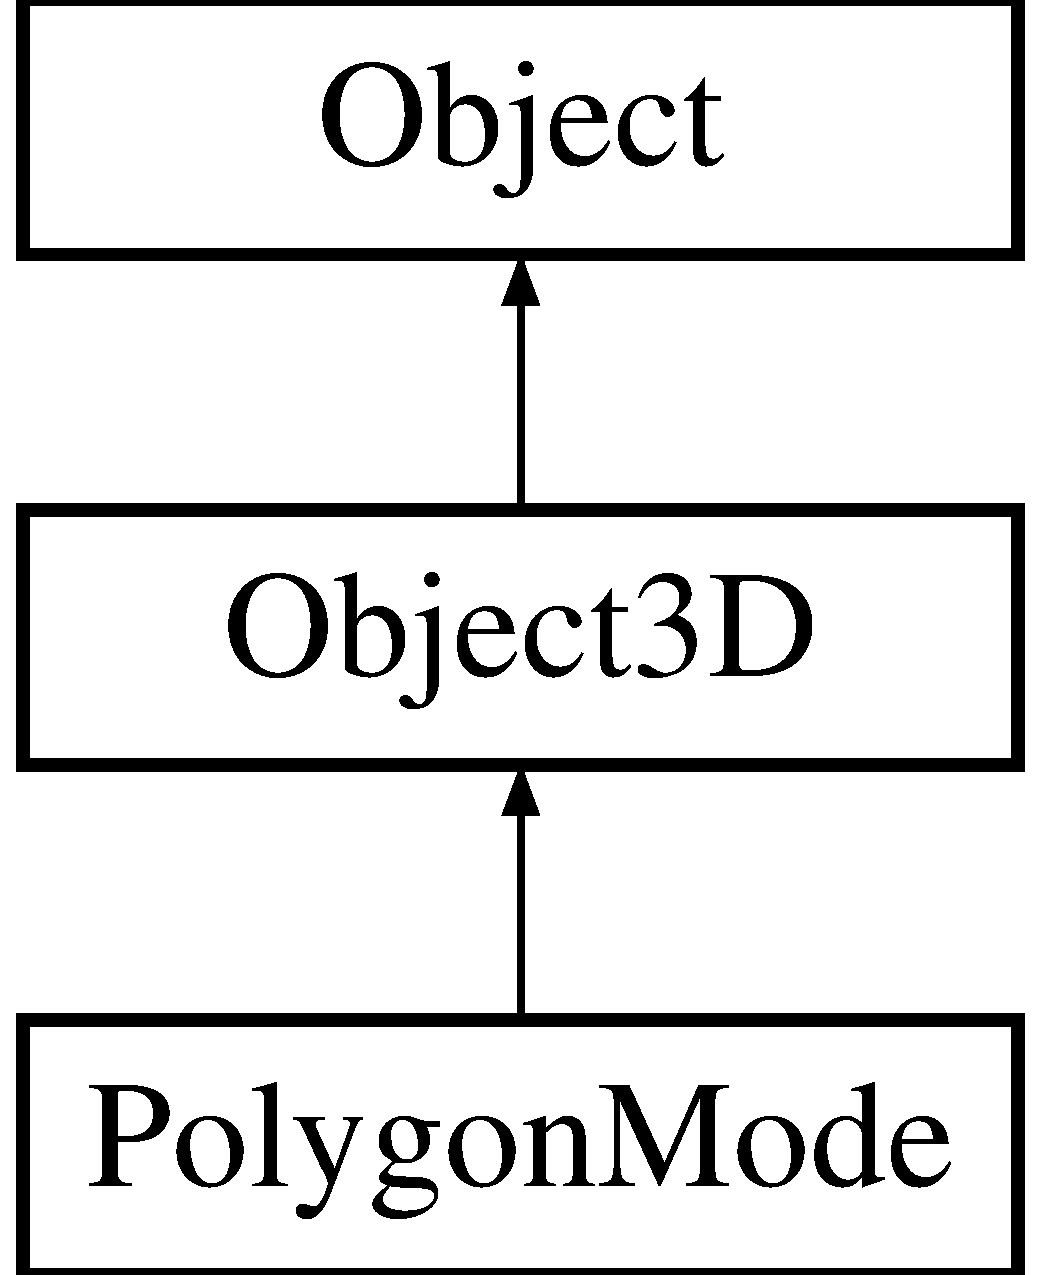
\includegraphics[height=3cm]{classm3g_1_1PolygonMode}
\end{center}
\end{figure}
\subsection*{Public メソッド}
\begin{CompactItemize}
\item 
\hyperlink{classm3g_1_1PolygonMode_b089ee808cbc4799bb2e92dd4ca554c3}{PolygonMode} ()
\item 
virtual \hyperlink{classm3g_1_1PolygonMode_64ea3958d7ec67fc648707782b2221fe}{$\sim$PolygonMode} ()
\item 
virtual \hyperlink{classm3g_1_1PolygonMode}{PolygonMode} $\ast$ \hyperlink{classm3g_1_1PolygonMode_a302cb097523e044bc03198ec8448c32}{duplicate} () const 
\item 
int \hyperlink{classm3g_1_1PolygonMode_3b0c0325e93774222d828f2612d59b1b}{getCulling} () const 
\item 
int \hyperlink{classm3g_1_1PolygonMode_c09a62f099e07df16a8c21f997b9f6a6}{getShading} () const 
\item 
int \hyperlink{classm3g_1_1PolygonMode_6000aac10def51a7c7f12e1381bce19d}{getWinding} () const 
\item 
bool \hyperlink{classm3g_1_1PolygonMode_b8db417fcee613ac80e84087046930cd}{isLocalCameraLightingEnabled} () const 
\item 
bool \hyperlink{classm3g_1_1PolygonMode_76ec871d6ed45e6e6a8822f5c45c828b}{isPerspectiveCorrectionEnabled} () const 
\item 
bool \hyperlink{classm3g_1_1PolygonMode_e7b9f0464063485b025f11a310bb0b80}{isTwoSidedLightingEnabled} () const 
\item 
void \hyperlink{classm3g_1_1PolygonMode_55b3fc23392376c00748d68bdf44ca60}{setCulling} (int mode)
\item 
void \hyperlink{classm3g_1_1PolygonMode_232d4cff53e6fc4863e144dc61e9465c}{setLocalCameraLightingEnable} (bool enable)
\item 
void \hyperlink{classm3g_1_1PolygonMode_81003e409298c3247ab2fed98a7270e9}{setPerspectiveCorrectionEnable} (bool enable)
\item 
void \hyperlink{classm3g_1_1PolygonMode_ebd2bc289af0e5cbee5ea29cbc55ba5a}{setShading} (int mode)
\item 
void \hyperlink{classm3g_1_1PolygonMode_8687b0d3016a777d32e7ebfa1ffd45aa}{setTwoSidedLightingEnable} (bool enable)
\item 
void \hyperlink{classm3g_1_1PolygonMode_5535581a651835a0da246b5936c2f0b5}{setWinding} (int mode)
\item 
virtual std::ostream \& \hyperlink{classm3g_1_1PolygonMode_6fea17fa1532df3794f8cb39cb4f911f}{print} (std::ostream \&out) const 
\item 
virtual void \hyperlink{classm3g_1_1PolygonMode_8babc8a79b78615da51161e94029eea9}{render} (\hyperlink{structm3g_1_1RenderState}{RenderState} \&state) const 
\end{CompactItemize}
\subsection*{Static Public メソッド}
\begin{CompactItemize}
\item 
static void \hyperlink{classm3g_1_1PolygonMode_443a7a301f77f625335ecc06d13bad06}{renderX} ()
\end{CompactItemize}
\subsection*{Static Public 変数}
\begin{CompactItemize}
\item 
static const int \hyperlink{classm3g_1_1PolygonMode_34ae9162b765ddbc1d2476edf3195361}{CULL\_\-BACK} = 160
\item 
static const int \hyperlink{classm3g_1_1PolygonMode_efa180528b010979c6f7732c3c3114ae}{CULL\_\-FRONT} = 161
\item 
static const int \hyperlink{classm3g_1_1PolygonMode_48717ad405f481d0f2ab8e948bf86822}{CULL\_\-NONE} = 162
\item 
static const int \hyperlink{classm3g_1_1PolygonMode_5da32249eba3f6eb4366f016c424099e}{SHADE\_\-FLAT} = 164
\item 
static const int \hyperlink{classm3g_1_1PolygonMode_2da5e6696c8e910d9fca74b583a081df}{SHADE\_\-SMOOTH} = 165
\item 
static const int \hyperlink{classm3g_1_1PolygonMode_98d881cf813edf483860268535014210}{WINDING\_\-CCW} = 168
\item 
static const int \hyperlink{classm3g_1_1PolygonMode_86975b3dec0d6cc20f54fd82eb13ef9e}{WINDING\_\-CW} = 169
\end{CompactItemize}


\subsection{説明}
ポリゴンレベルの属性値をカプセル化したアピアランスの構成要素. 

\subsection{コンストラクタとデストラクタ}
\hypertarget{classm3g_1_1PolygonMode_b089ee808cbc4799bb2e92dd4ca554c3}{
\index{m3g::PolygonMode@{m3g::PolygonMode}!PolygonMode@{PolygonMode}}
\index{PolygonMode@{PolygonMode}!m3g::PolygonMode@{m3g::PolygonMode}}
\subsubsection[{PolygonMode}]{\setlength{\rightskip}{0pt plus 5cm}{\bf PolygonMode} ()}}
\label{classm3g_1_1PolygonMode_b089ee808cbc4799bb2e92dd4ca554c3}


デフォルト値でPolygonModeオブジェクトの作成. \hypertarget{classm3g_1_1PolygonMode_64ea3958d7ec67fc648707782b2221fe}{
\index{m3g::PolygonMode@{m3g::PolygonMode}!$\sim$PolygonMode@{$\sim$PolygonMode}}
\index{$\sim$PolygonMode@{$\sim$PolygonMode}!m3g::PolygonMode@{m3g::PolygonMode}}
\subsubsection[{$\sim$PolygonMode}]{\setlength{\rightskip}{0pt plus 5cm}$\sim${\bf PolygonMode} ()\hspace{0.3cm}{\tt  \mbox{[}virtual\mbox{]}}}}
\label{classm3g_1_1PolygonMode_64ea3958d7ec67fc648707782b2221fe}


このオブジェクトを削除するデストラクタ. 

\subsection{関数}
\hypertarget{classm3g_1_1PolygonMode_a302cb097523e044bc03198ec8448c32}{
\index{m3g::PolygonMode@{m3g::PolygonMode}!duplicate@{duplicate}}
\index{duplicate@{duplicate}!m3g::PolygonMode@{m3g::PolygonMode}}
\subsubsection[{duplicate}]{\setlength{\rightskip}{0pt plus 5cm}{\bf PolygonMode} $\ast$ duplicate () const\hspace{0.3cm}{\tt  \mbox{[}virtual\mbox{]}}}}
\label{classm3g_1_1PolygonMode_a302cb097523e044bc03198ec8448c32}


このオブジェクトの複製の作成. 

\hyperlink{classm3g_1_1Object3D_a25110dac934f867b83b73ad4741a0f4}{Object3D}を再定義しています。\hypertarget{classm3g_1_1PolygonMode_3b0c0325e93774222d828f2612d59b1b}{
\index{m3g::PolygonMode@{m3g::PolygonMode}!getCulling@{getCulling}}
\index{getCulling@{getCulling}!m3g::PolygonMode@{m3g::PolygonMode}}
\subsubsection[{getCulling}]{\setlength{\rightskip}{0pt plus 5cm}int getCulling () const}}
\label{classm3g_1_1PolygonMode_3b0c0325e93774222d828f2612d59b1b}


カレントのポリゴンのカリングモードの取得. \hypertarget{classm3g_1_1PolygonMode_c09a62f099e07df16a8c21f997b9f6a6}{
\index{m3g::PolygonMode@{m3g::PolygonMode}!getShading@{getShading}}
\index{getShading@{getShading}!m3g::PolygonMode@{m3g::PolygonMode}}
\subsubsection[{getShading}]{\setlength{\rightskip}{0pt plus 5cm}int getShading () const}}
\label{classm3g_1_1PolygonMode_c09a62f099e07df16a8c21f997b9f6a6}


ポリゴンのシェーディングモードの取得. \hypertarget{classm3g_1_1PolygonMode_6000aac10def51a7c7f12e1381bce19d}{
\index{m3g::PolygonMode@{m3g::PolygonMode}!getWinding@{getWinding}}
\index{getWinding@{getWinding}!m3g::PolygonMode@{m3g::PolygonMode}}
\subsubsection[{getWinding}]{\setlength{\rightskip}{0pt plus 5cm}int getWinding () const}}
\label{classm3g_1_1PolygonMode_6000aac10def51a7c7f12e1381bce19d}


ポリゴンのワインでぃんぐもーどの取得. \hypertarget{classm3g_1_1PolygonMode_b8db417fcee613ac80e84087046930cd}{
\index{m3g::PolygonMode@{m3g::PolygonMode}!isLocalCameraLightingEnabled@{isLocalCameraLightingEnabled}}
\index{isLocalCameraLightingEnabled@{isLocalCameraLightingEnabled}!m3g::PolygonMode@{m3g::PolygonMode}}
\subsubsection[{isLocalCameraLightingEnabled}]{\setlength{\rightskip}{0pt plus 5cm}bool isLocalCameraLightingEnabled () const}}
\label{classm3g_1_1PolygonMode_b8db417fcee613ac80e84087046930cd}


ローカルカメラライティングの有効、無効の取得. \hypertarget{classm3g_1_1PolygonMode_76ec871d6ed45e6e6a8822f5c45c828b}{
\index{m3g::PolygonMode@{m3g::PolygonMode}!isPerspectiveCorrectionEnabled@{isPerspectiveCorrectionEnabled}}
\index{isPerspectiveCorrectionEnabled@{isPerspectiveCorrectionEnabled}!m3g::PolygonMode@{m3g::PolygonMode}}
\subsubsection[{isPerspectiveCorrectionEnabled}]{\setlength{\rightskip}{0pt plus 5cm}bool isPerspectiveCorrectionEnabled () const}}
\label{classm3g_1_1PolygonMode_76ec871d6ed45e6e6a8822f5c45c828b}


透視変換補正の有効、無効の問い合わせ. \hypertarget{classm3g_1_1PolygonMode_e7b9f0464063485b025f11a310bb0b80}{
\index{m3g::PolygonMode@{m3g::PolygonMode}!isTwoSidedLightingEnabled@{isTwoSidedLightingEnabled}}
\index{isTwoSidedLightingEnabled@{isTwoSidedLightingEnabled}!m3g::PolygonMode@{m3g::PolygonMode}}
\subsubsection[{isTwoSidedLightingEnabled}]{\setlength{\rightskip}{0pt plus 5cm}bool isTwoSidedLightingEnabled () const}}
\label{classm3g_1_1PolygonMode_e7b9f0464063485b025f11a310bb0b80}


両面ライティングの有効、無効の問い合わせ. \hypertarget{classm3g_1_1PolygonMode_6fea17fa1532df3794f8cb39cb4f911f}{
\index{m3g::PolygonMode@{m3g::PolygonMode}!print@{print}}
\index{print@{print}!m3g::PolygonMode@{m3g::PolygonMode}}
\subsubsection[{print}]{\setlength{\rightskip}{0pt plus 5cm}std::ostream \& print (std::ostream \& {\em out}) const\hspace{0.3cm}{\tt  \mbox{[}virtual\mbox{]}}}}
\label{classm3g_1_1PolygonMode_6fea17fa1532df3794f8cb39cb4f911f}


このPolygoModeの情報を表示する。デバッグ用. 

\hyperlink{classm3g_1_1Object3D_6fea17fa1532df3794f8cb39cb4f911f}{Object3D}を再定義しています。\hypertarget{classm3g_1_1PolygonMode_8babc8a79b78615da51161e94029eea9}{
\index{m3g::PolygonMode@{m3g::PolygonMode}!render@{render}}
\index{render@{render}!m3g::PolygonMode@{m3g::PolygonMode}}
\subsubsection[{render}]{\setlength{\rightskip}{0pt plus 5cm}void render ({\bf RenderState} \& {\em state}) const\hspace{0.3cm}{\tt  \mbox{[}virtual\mbox{]}}}}
\label{classm3g_1_1PolygonMode_8babc8a79b78615da51161e94029eea9}


このオブジェクトをレンダリングする内部使用の関数. 

\hyperlink{classm3g_1_1Object3D_8babc8a79b78615da51161e94029eea9}{Object3D}を再定義しています。\hypertarget{classm3g_1_1PolygonMode_443a7a301f77f625335ecc06d13bad06}{
\index{m3g::PolygonMode@{m3g::PolygonMode}!renderX@{renderX}}
\index{renderX@{renderX}!m3g::PolygonMode@{m3g::PolygonMode}}
\subsubsection[{renderX}]{\setlength{\rightskip}{0pt plus 5cm}void renderX ()\hspace{0.3cm}{\tt  \mbox{[}static\mbox{]}}}}
\label{classm3g_1_1PolygonMode_443a7a301f77f625335ecc06d13bad06}


デフォルトでレンダリングする内部使用の関数. \hypertarget{classm3g_1_1PolygonMode_55b3fc23392376c00748d68bdf44ca60}{
\index{m3g::PolygonMode@{m3g::PolygonMode}!setCulling@{setCulling}}
\index{setCulling@{setCulling}!m3g::PolygonMode@{m3g::PolygonMode}}
\subsubsection[{setCulling}]{\setlength{\rightskip}{0pt plus 5cm}void setCulling (int {\em mode})}}
\label{classm3g_1_1PolygonMode_55b3fc23392376c00748d68bdf44ca60}


ポリゴンのカリングモードの設定. \hypertarget{classm3g_1_1PolygonMode_232d4cff53e6fc4863e144dc61e9465c}{
\index{m3g::PolygonMode@{m3g::PolygonMode}!setLocalCameraLightingEnable@{setLocalCameraLightingEnable}}
\index{setLocalCameraLightingEnable@{setLocalCameraLightingEnable}!m3g::PolygonMode@{m3g::PolygonMode}}
\subsubsection[{setLocalCameraLightingEnable}]{\setlength{\rightskip}{0pt plus 5cm}void setLocalCameraLightingEnable (bool {\em enable})}}
\label{classm3g_1_1PolygonMode_232d4cff53e6fc4863e144dc61e9465c}


ローカルカメラライティングの有効化、無効化. \hypertarget{classm3g_1_1PolygonMode_81003e409298c3247ab2fed98a7270e9}{
\index{m3g::PolygonMode@{m3g::PolygonMode}!setPerspectiveCorrectionEnable@{setPerspectiveCorrectionEnable}}
\index{setPerspectiveCorrectionEnable@{setPerspectiveCorrectionEnable}!m3g::PolygonMode@{m3g::PolygonMode}}
\subsubsection[{setPerspectiveCorrectionEnable}]{\setlength{\rightskip}{0pt plus 5cm}void setPerspectiveCorrectionEnable (bool {\em enable})}}
\label{classm3g_1_1PolygonMode_81003e409298c3247ab2fed98a7270e9}


透視変換補正の有効化、無効化. \hypertarget{classm3g_1_1PolygonMode_ebd2bc289af0e5cbee5ea29cbc55ba5a}{
\index{m3g::PolygonMode@{m3g::PolygonMode}!setShading@{setShading}}
\index{setShading@{setShading}!m3g::PolygonMode@{m3g::PolygonMode}}
\subsubsection[{setShading}]{\setlength{\rightskip}{0pt plus 5cm}void setShading (int {\em mode})}}
\label{classm3g_1_1PolygonMode_ebd2bc289af0e5cbee5ea29cbc55ba5a}


ポリゴンのシェーディングモードの設定. \hypertarget{classm3g_1_1PolygonMode_8687b0d3016a777d32e7ebfa1ffd45aa}{
\index{m3g::PolygonMode@{m3g::PolygonMode}!setTwoSidedLightingEnable@{setTwoSidedLightingEnable}}
\index{setTwoSidedLightingEnable@{setTwoSidedLightingEnable}!m3g::PolygonMode@{m3g::PolygonMode}}
\subsubsection[{setTwoSidedLightingEnable}]{\setlength{\rightskip}{0pt plus 5cm}void setTwoSidedLightingEnable (bool {\em enable})}}
\label{classm3g_1_1PolygonMode_8687b0d3016a777d32e7ebfa1ffd45aa}


両面ライティングの有効化、無効化. \hypertarget{classm3g_1_1PolygonMode_5535581a651835a0da246b5936c2f0b5}{
\index{m3g::PolygonMode@{m3g::PolygonMode}!setWinding@{setWinding}}
\index{setWinding@{setWinding}!m3g::PolygonMode@{m3g::PolygonMode}}
\subsubsection[{setWinding}]{\setlength{\rightskip}{0pt plus 5cm}void setWinding (int {\em mode})}}
\label{classm3g_1_1PolygonMode_5535581a651835a0da246b5936c2f0b5}


ポリゴンのワインディングモードを時計回りか、反時計回りに設定する. 

\subsection{変数}
\hypertarget{classm3g_1_1PolygonMode_34ae9162b765ddbc1d2476edf3195361}{
\index{m3g::PolygonMode@{m3g::PolygonMode}!CULL\_\-BACK@{CULL\_\-BACK}}
\index{CULL\_\-BACK@{CULL\_\-BACK}!m3g::PolygonMode@{m3g::PolygonMode}}
\subsubsection[{CULL\_\-BACK}]{\setlength{\rightskip}{0pt plus 5cm}const int {\bf CULL\_\-BACK} = 160\hspace{0.3cm}{\tt  \mbox{[}static\mbox{]}}}}
\label{classm3g_1_1PolygonMode_34ae9162b765ddbc1d2476edf3195361}


背面のカリングを表す定数. \hypertarget{classm3g_1_1PolygonMode_efa180528b010979c6f7732c3c3114ae}{
\index{m3g::PolygonMode@{m3g::PolygonMode}!CULL\_\-FRONT@{CULL\_\-FRONT}}
\index{CULL\_\-FRONT@{CULL\_\-FRONT}!m3g::PolygonMode@{m3g::PolygonMode}}
\subsubsection[{CULL\_\-FRONT}]{\setlength{\rightskip}{0pt plus 5cm}const int {\bf CULL\_\-FRONT} = 161\hspace{0.3cm}{\tt  \mbox{[}static\mbox{]}}}}
\label{classm3g_1_1PolygonMode_efa180528b010979c6f7732c3c3114ae}


前面のカリングを表す定数. \hypertarget{classm3g_1_1PolygonMode_48717ad405f481d0f2ab8e948bf86822}{
\index{m3g::PolygonMode@{m3g::PolygonMode}!CULL\_\-NONE@{CULL\_\-NONE}}
\index{CULL\_\-NONE@{CULL\_\-NONE}!m3g::PolygonMode@{m3g::PolygonMode}}
\subsubsection[{CULL\_\-NONE}]{\setlength{\rightskip}{0pt plus 5cm}const int {\bf CULL\_\-NONE} = 162\hspace{0.3cm}{\tt  \mbox{[}static\mbox{]}}}}
\label{classm3g_1_1PolygonMode_48717ad405f481d0f2ab8e948bf86822}


カリングなしを表す定数. \hypertarget{classm3g_1_1PolygonMode_5da32249eba3f6eb4366f016c424099e}{
\index{m3g::PolygonMode@{m3g::PolygonMode}!SHADE\_\-FLAT@{SHADE\_\-FLAT}}
\index{SHADE\_\-FLAT@{SHADE\_\-FLAT}!m3g::PolygonMode@{m3g::PolygonMode}}
\subsubsection[{SHADE\_\-FLAT}]{\setlength{\rightskip}{0pt plus 5cm}const int {\bf SHADE\_\-FLAT} = 164\hspace{0.3cm}{\tt  \mbox{[}static\mbox{]}}}}
\label{classm3g_1_1PolygonMode_5da32249eba3f6eb4366f016c424099e}


フラットシェーディングを表す定数. \hypertarget{classm3g_1_1PolygonMode_2da5e6696c8e910d9fca74b583a081df}{
\index{m3g::PolygonMode@{m3g::PolygonMode}!SHADE\_\-SMOOTH@{SHADE\_\-SMOOTH}}
\index{SHADE\_\-SMOOTH@{SHADE\_\-SMOOTH}!m3g::PolygonMode@{m3g::PolygonMode}}
\subsubsection[{SHADE\_\-SMOOTH}]{\setlength{\rightskip}{0pt plus 5cm}const int {\bf SHADE\_\-SMOOTH} = 165\hspace{0.3cm}{\tt  \mbox{[}static\mbox{]}}}}
\label{classm3g_1_1PolygonMode_2da5e6696c8e910d9fca74b583a081df}


スムースシェーディングを表す定数. \hypertarget{classm3g_1_1PolygonMode_98d881cf813edf483860268535014210}{
\index{m3g::PolygonMode@{m3g::PolygonMode}!WINDING\_\-CCW@{WINDING\_\-CCW}}
\index{WINDING\_\-CCW@{WINDING\_\-CCW}!m3g::PolygonMode@{m3g::PolygonMode}}
\subsubsection[{WINDING\_\-CCW}]{\setlength{\rightskip}{0pt plus 5cm}const int {\bf WINDING\_\-CCW} = 168\hspace{0.3cm}{\tt  \mbox{[}static\mbox{]}}}}
\label{classm3g_1_1PolygonMode_98d881cf813edf483860268535014210}


反時計回りの頂点の並び順を前面と規定する定数. \hypertarget{classm3g_1_1PolygonMode_86975b3dec0d6cc20f54fd82eb13ef9e}{
\index{m3g::PolygonMode@{m3g::PolygonMode}!WINDING\_\-CW@{WINDING\_\-CW}}
\index{WINDING\_\-CW@{WINDING\_\-CW}!m3g::PolygonMode@{m3g::PolygonMode}}
\subsubsection[{WINDING\_\-CW}]{\setlength{\rightskip}{0pt plus 5cm}const int {\bf WINDING\_\-CW} = 169\hspace{0.3cm}{\tt  \mbox{[}static\mbox{]}}}}
\label{classm3g_1_1PolygonMode_86975b3dec0d6cc20f54fd82eb13ef9e}


時計回りの頂点の並び順を前面と規定する定数. 

このクラスの説明は次のファイルから生成されました:\begin{CompactItemize}
\item 
/work/workspace.desktop-m3g/src/PolygonMode.hpp\item 
/work/workspace.desktop-m3g/src/PolygonMode.cpp\end{CompactItemize}

\hypertarget{classm3g_1_1Quaternion}{
\section{クラス Quaternion}
\label{classm3g_1_1Quaternion}\index{m3g::Quaternion@{m3g::Quaternion}}
}
{\tt \#include $<$Quaternion.hpp$>$}

\subsection*{Public メソッド}
\begin{CompactItemize}
\item 
\hyperlink{classm3g_1_1Quaternion_65ed15cc19af958b5933b5c522f10e66}{Quaternion} ()
\item 
\hyperlink{classm3g_1_1Quaternion_7a06a28b864e525f73a1bb0eb3e9274e}{Quaternion} (float angle, float ax, float ay, float az)
\item 
\hyperlink{classm3g_1_1Quaternion_6e9a147677b9ffd583c59e9d06c3d938}{$\sim$Quaternion} ()
\item 
void \hyperlink{classm3g_1_1Quaternion_382e6ad7e6721b121e510959e1011be3}{setIdentity} ()
\item 
void \hyperlink{classm3g_1_1Quaternion_47affd1a10b589811fc4828c1a2e0c6d}{setZero} ()
\item 
\hyperlink{classm3g_1_1Quaternion}{Quaternion} \& \hyperlink{classm3g_1_1Quaternion_c9cc178bcc449e08499113c35feb2a2b}{normalize} ()
\item 
void \hyperlink{classm3g_1_1Quaternion_0712dc357557a30ac0da0a9d4cdd278c}{set} (float qx, float qy, float qz, float qw)
\item 
void \hyperlink{classm3g_1_1Quaternion_3049675269aef6bb333d8f83fdf6eed7}{getAngleAxis} (float $\ast$angle\_\-axis) const 
\item 
float \hyperlink{classm3g_1_1Quaternion_b4393f1928cea2a3baadbf9acdd99de2}{getLength} () const 
\item 
std::ostream \& \hyperlink{classm3g_1_1Quaternion_6fea17fa1532df3794f8cb39cb4f911f}{print} (std::ostream \&out) const 
\end{CompactItemize}
\subsection*{Public 変数}
\begin{CompactItemize}
\item 
\hypertarget{classm3g_1_1Quaternion_d0da36b2558901e21e7a30f6c227a45e}{
float \textbf{x}}
\label{classm3g_1_1Quaternion_d0da36b2558901e21e7a30f6c227a45e}

\item 
\hypertarget{classm3g_1_1Quaternion_a4f0d3eebc3c443f9be81bf48561a217}{
float \textbf{y}}
\label{classm3g_1_1Quaternion_a4f0d3eebc3c443f9be81bf48561a217}

\item 
\hypertarget{classm3g_1_1Quaternion_f73583b1e980b0aa03f9884812e9fd4d}{
float \textbf{z}}
\label{classm3g_1_1Quaternion_f73583b1e980b0aa03f9884812e9fd4d}

\item 
\hypertarget{classm3g_1_1Quaternion_56eca241e2896b9f57a79589e76fd24b}{
float \textbf{w}}
\label{classm3g_1_1Quaternion_56eca241e2896b9f57a79589e76fd24b}

\end{CompactItemize}


\subsection{説明}
回転を表すクォータニオンクラス。内部使用専用. 

\subsection{コンストラクタとデストラクタ}
\hypertarget{classm3g_1_1Quaternion_65ed15cc19af958b5933b5c522f10e66}{
\index{m3g::Quaternion@{m3g::Quaternion}!Quaternion@{Quaternion}}
\index{Quaternion@{Quaternion}!m3g::Quaternion@{m3g::Quaternion}}
\subsubsection[{Quaternion}]{\setlength{\rightskip}{0pt plus 5cm}{\bf Quaternion} ()}}
\label{classm3g_1_1Quaternion_65ed15cc19af958b5933b5c522f10e66}


単位クォータニオンを作成するコンストラクタ. \hypertarget{classm3g_1_1Quaternion_7a06a28b864e525f73a1bb0eb3e9274e}{
\index{m3g::Quaternion@{m3g::Quaternion}!Quaternion@{Quaternion}}
\index{Quaternion@{Quaternion}!m3g::Quaternion@{m3g::Quaternion}}
\subsubsection[{Quaternion}]{\setlength{\rightskip}{0pt plus 5cm}{\bf Quaternion} (float {\em angle}, \/  float {\em ax}, \/  float {\em ay}, \/  float {\em az})}}
\label{classm3g_1_1Quaternion_7a06a28b864e525f73a1bb0eb3e9274e}


回転角度、回転軸の形式でクォータニオンを作成するコンストラクタ。 回転軸は正規化されている必要はない. \hypertarget{classm3g_1_1Quaternion_6e9a147677b9ffd583c59e9d06c3d938}{
\index{m3g::Quaternion@{m3g::Quaternion}!$\sim$Quaternion@{$\sim$Quaternion}}
\index{$\sim$Quaternion@{$\sim$Quaternion}!m3g::Quaternion@{m3g::Quaternion}}
\subsubsection[{$\sim$Quaternion}]{\setlength{\rightskip}{0pt plus 5cm}$\sim${\bf Quaternion} ()}}
\label{classm3g_1_1Quaternion_6e9a147677b9ffd583c59e9d06c3d938}


このオブジェクトを削除するデストラクタ. 

\subsection{関数}
\hypertarget{classm3g_1_1Quaternion_3049675269aef6bb333d8f83fdf6eed7}{
\index{m3g::Quaternion@{m3g::Quaternion}!getAngleAxis@{getAngleAxis}}
\index{getAngleAxis@{getAngleAxis}!m3g::Quaternion@{m3g::Quaternion}}
\subsubsection[{getAngleAxis}]{\setlength{\rightskip}{0pt plus 5cm}void getAngleAxis (float $\ast$ {\em angle\_\-axis}) const}}
\label{classm3g_1_1Quaternion_3049675269aef6bb333d8f83fdf6eed7}


このクォータニオンを角度-回転軸の形式で取得.

(補足) 回転角度が0の場合はangle=0,axis=(x,y,z)が返る. \hypertarget{classm3g_1_1Quaternion_b4393f1928cea2a3baadbf9acdd99de2}{
\index{m3g::Quaternion@{m3g::Quaternion}!getLength@{getLength}}
\index{getLength@{getLength}!m3g::Quaternion@{m3g::Quaternion}}
\subsubsection[{getLength}]{\setlength{\rightskip}{0pt plus 5cm}float getLength () const}}
\label{classm3g_1_1Quaternion_b4393f1928cea2a3baadbf9acdd99de2}


このクォータニオンを長さを取得. \hypertarget{classm3g_1_1Quaternion_c9cc178bcc449e08499113c35feb2a2b}{
\index{m3g::Quaternion@{m3g::Quaternion}!normalize@{normalize}}
\index{normalize@{normalize}!m3g::Quaternion@{m3g::Quaternion}}
\subsubsection[{normalize}]{\setlength{\rightskip}{0pt plus 5cm}{\bf Quaternion} \& normalize ()}}
\label{classm3g_1_1Quaternion_c9cc178bcc449e08499113c35feb2a2b}


クォータニオンを正規化化する. \hypertarget{classm3g_1_1Quaternion_6fea17fa1532df3794f8cb39cb4f911f}{
\index{m3g::Quaternion@{m3g::Quaternion}!print@{print}}
\index{print@{print}!m3g::Quaternion@{m3g::Quaternion}}
\subsubsection[{print}]{\setlength{\rightskip}{0pt plus 5cm}std::ostream \& print (std::ostream \& {\em out}) const}}
\label{classm3g_1_1Quaternion_6fea17fa1532df3794f8cb39cb4f911f}


このオブジェクトの情報を表示する。デバッグ用. \hypertarget{classm3g_1_1Quaternion_0712dc357557a30ac0da0a9d4cdd278c}{
\index{m3g::Quaternion@{m3g::Quaternion}!set@{set}}
\index{set@{set}!m3g::Quaternion@{m3g::Quaternion}}
\subsubsection[{set}]{\setlength{\rightskip}{0pt plus 5cm}void set (float {\em qx}, \/  float {\em qy}, \/  float {\em qz}, \/  float {\em qw})}}
\label{classm3g_1_1Quaternion_0712dc357557a30ac0da0a9d4cdd278c}


クォータニオンを設定する。関数内部で正規化される. \hypertarget{classm3g_1_1Quaternion_382e6ad7e6721b121e510959e1011be3}{
\index{m3g::Quaternion@{m3g::Quaternion}!setIdentity@{setIdentity}}
\index{setIdentity@{setIdentity}!m3g::Quaternion@{m3g::Quaternion}}
\subsubsection[{setIdentity}]{\setlength{\rightskip}{0pt plus 5cm}void setIdentity ()}}
\label{classm3g_1_1Quaternion_382e6ad7e6721b121e510959e1011be3}


単位クォータニオン化する. \hypertarget{classm3g_1_1Quaternion_47affd1a10b589811fc4828c1a2e0c6d}{
\index{m3g::Quaternion@{m3g::Quaternion}!setZero@{setZero}}
\index{setZero@{setZero}!m3g::Quaternion@{m3g::Quaternion}}
\subsubsection[{setZero}]{\setlength{\rightskip}{0pt plus 5cm}void setZero ()}}
\label{classm3g_1_1Quaternion_47affd1a10b589811fc4828c1a2e0c6d}


クォータニオンをゼロ化する. 

このクラスの説明は次のファイルから生成されました:\begin{CompactItemize}
\item 
/work/workspace.desktop-m3g/src/Quaternion.hpp\item 
/work/workspace.desktop-m3g/src/Quaternion.cpp\end{CompactItemize}

\hypertarget{classm3g_1_1RayIntersection}{
\section{クラス RayIntersection}
\label{classm3g_1_1RayIntersection}\index{m3g::RayIntersection@{m3g::RayIntersection}}
}
{\tt \#include $<$RayIntersection.hpp$>$}

RayIntersectionに対する継承グラフ:\begin{figure}[H]
\begin{center}
\leavevmode
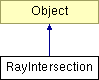
\includegraphics[height=2cm]{classm3g_1_1RayIntersection}
\end{center}
\end{figure}
\subsection*{構成}
\begin{CompactItemize}
\item 
struct \textbf{Ray}
\end{CompactItemize}
\subsection*{Public メソッド}
\begin{CompactItemize}
\item 
\hyperlink{classm3g_1_1RayIntersection_242b33a79f98ed90ad5a36912d2a46d5}{RayIntersection} ()
\item 
\hyperlink{classm3g_1_1RayIntersection_c7d946885706d0cefed30d9ee257a771}{RayIntersection} (\hyperlink{classm3g_1_1Node}{Node} $\ast$node, const \hyperlink{classm3g_1_1Vector}{Vector} \&org, const \hyperlink{classm3g_1_1Vector}{Vector} \&dir, float t, float u, float v, int vertex\_\-num, int $\ast$vertices, int submesh\_\-index)
\item 
\hyperlink{classm3g_1_1RayIntersection_bf9eb45cc9ff31acd542bb0da1b46fe1}{$\sim$RayIntersection} ()
\item 
float \hyperlink{classm3g_1_1RayIntersection_f024301f51d2ef67cac50e3255a49612}{getDistance} () const 
\item 
\hyperlink{classm3g_1_1Node}{Node} $\ast$ \hyperlink{classm3g_1_1RayIntersection_cbf90cea6001c33cc03b5a737b312f62}{getIntersected} () const 
\item 
float \hyperlink{classm3g_1_1RayIntersection_0ee7a8fab5e001b131bd3109da8af7fa}{getNormalX} () const 
\item 
float \hyperlink{classm3g_1_1RayIntersection_1e05e3b3e8d6b46462812e4713a63d18}{getNormalY} () const 
\item 
float \hyperlink{classm3g_1_1RayIntersection_5d0569741397401f53b776f16d08f5c3}{getNormalZ} () const 
\item 
void \hyperlink{classm3g_1_1RayIntersection_3f4d1f2f24c0dadab914014836e1b138}{getRay} (float $\ast$ray) const 
\item 
int \hyperlink{classm3g_1_1RayIntersection_6a11c61d1a1fecc01f2f83463404a6b8}{getSubmeshIndex} () const 
\item 
float \hyperlink{classm3g_1_1RayIntersection_bc14e1d5a83d5fca608b1fbf772614d4}{getTextureS} (int index) const 
\item 
float \hyperlink{classm3g_1_1RayIntersection_843d5b907bb54a6f28571f0a0f14c932}{getTextureT} (int index) const 
\item 
void \hyperlink{classm3g_1_1RayIntersection_ee558b3e4c2a54d66f2bb47e3dea6188}{transformRay} (const \hyperlink{classm3g_1_1Transform}{Transform} \&trans)
\item 
std::ostream \& \hyperlink{classm3g_1_1RayIntersection_6fea17fa1532df3794f8cb39cb4f911f}{print} (std::ostream \&out) const 
\end{CompactItemize}


\subsection{説明}
Groupのpick関数によって生成され、交差点の情報を収納するクラス. 

\subsection{コンストラクタとデストラクタ}
\hypertarget{classm3g_1_1RayIntersection_242b33a79f98ed90ad5a36912d2a46d5}{
\index{m3g::RayIntersection@{m3g::RayIntersection}!RayIntersection@{RayIntersection}}
\index{RayIntersection@{RayIntersection}!m3g::RayIntersection@{m3g::RayIntersection}}
\subsubsection[{RayIntersection}]{\setlength{\rightskip}{0pt plus 5cm}{\bf RayIntersection} ()}}
\label{classm3g_1_1RayIntersection_242b33a79f98ed90ad5a36912d2a46d5}


デフォルト値のコンストラクタ. \hypertarget{classm3g_1_1RayIntersection_c7d946885706d0cefed30d9ee257a771}{
\index{m3g::RayIntersection@{m3g::RayIntersection}!RayIntersection@{RayIntersection}}
\index{RayIntersection@{RayIntersection}!m3g::RayIntersection@{m3g::RayIntersection}}
\subsubsection[{RayIntersection}]{\setlength{\rightskip}{0pt plus 5cm}{\bf RayIntersection} ({\bf Node} $\ast$ {\em node}, \/  const {\bf Vector} \& {\em org}, \/  const {\bf Vector} \& {\em dir}, \/  float {\em t}, \/  float {\em u}, \/  float {\em v}, \/  int {\em vertex\_\-num}, \/  int $\ast$ {\em vertices}, \/  int {\em submesh\_\-index})}}
\label{classm3g_1_1RayIntersection_c7d946885706d0cefed30d9ee257a771}


M3G未定義. 第1引数はNodeではなくMeshの方が良いか? \hypertarget{classm3g_1_1RayIntersection_bf9eb45cc9ff31acd542bb0da1b46fe1}{
\index{m3g::RayIntersection@{m3g::RayIntersection}!$\sim$RayIntersection@{$\sim$RayIntersection}}
\index{$\sim$RayIntersection@{$\sim$RayIntersection}!m3g::RayIntersection@{m3g::RayIntersection}}
\subsubsection[{$\sim$RayIntersection}]{\setlength{\rightskip}{0pt plus 5cm}$\sim${\bf RayIntersection} ()}}
\label{classm3g_1_1RayIntersection_bf9eb45cc9ff31acd542bb0da1b46fe1}


このオブジェクトを削除するデストラクタ. 

\subsection{関数}
\hypertarget{classm3g_1_1RayIntersection_f024301f51d2ef67cac50e3255a49612}{
\index{m3g::RayIntersection@{m3g::RayIntersection}!getDistance@{getDistance}}
\index{getDistance@{getDistance}!m3g::RayIntersection@{m3g::RayIntersection}}
\subsubsection[{getDistance}]{\setlength{\rightskip}{0pt plus 5cm}float getDistance () const}}
\label{classm3g_1_1RayIntersection_f024301f51d2ef67cac50e3255a49612}


ピック光線の交差地点までの距離を取得する. \hypertarget{classm3g_1_1RayIntersection_cbf90cea6001c33cc03b5a737b312f62}{
\index{m3g::RayIntersection@{m3g::RayIntersection}!getIntersected@{getIntersected}}
\index{getIntersected@{getIntersected}!m3g::RayIntersection@{m3g::RayIntersection}}
\subsubsection[{getIntersected}]{\setlength{\rightskip}{0pt plus 5cm}{\bf Node} $\ast$ getIntersected () const}}
\label{classm3g_1_1RayIntersection_cbf90cea6001c33cc03b5a737b312f62}


ピックされたMeshまたはSprite3Dクラスを取得する. \hypertarget{classm3g_1_1RayIntersection_0ee7a8fab5e001b131bd3109da8af7fa}{
\index{m3g::RayIntersection@{m3g::RayIntersection}!getNormalX@{getNormalX}}
\index{getNormalX@{getNormalX}!m3g::RayIntersection@{m3g::RayIntersection}}
\subsubsection[{getNormalX}]{\setlength{\rightskip}{0pt plus 5cm}float getNormalX () const}}
\label{classm3g_1_1RayIntersection_0ee7a8fab5e001b131bd3109da8af7fa}


交差地点のサーフェス法線のXコンポーネントの取得. \hypertarget{classm3g_1_1RayIntersection_1e05e3b3e8d6b46462812e4713a63d18}{
\index{m3g::RayIntersection@{m3g::RayIntersection}!getNormalY@{getNormalY}}
\index{getNormalY@{getNormalY}!m3g::RayIntersection@{m3g::RayIntersection}}
\subsubsection[{getNormalY}]{\setlength{\rightskip}{0pt plus 5cm}float getNormalY () const}}
\label{classm3g_1_1RayIntersection_1e05e3b3e8d6b46462812e4713a63d18}


交差地点のサーフェス法線のYコンポーネントの取得. \hypertarget{classm3g_1_1RayIntersection_5d0569741397401f53b776f16d08f5c3}{
\index{m3g::RayIntersection@{m3g::RayIntersection}!getNormalZ@{getNormalZ}}
\index{getNormalZ@{getNormalZ}!m3g::RayIntersection@{m3g::RayIntersection}}
\subsubsection[{getNormalZ}]{\setlength{\rightskip}{0pt plus 5cm}float getNormalZ () const}}
\label{classm3g_1_1RayIntersection_5d0569741397401f53b776f16d08f5c3}


交差地点のサーフェス法線のZコンポーネントの取得. \hypertarget{classm3g_1_1RayIntersection_3f4d1f2f24c0dadab914014836e1b138}{
\index{m3g::RayIntersection@{m3g::RayIntersection}!getRay@{getRay}}
\index{getRay@{getRay}!m3g::RayIntersection@{m3g::RayIntersection}}
\subsubsection[{getRay}]{\setlength{\rightskip}{0pt plus 5cm}void getRay (float $\ast$ {\em ray}) const}}
\label{classm3g_1_1RayIntersection_3f4d1f2f24c0dadab914014836e1b138}


ピック光線の原点(ox,oy,oz)、方向(dx,dy,dz)を取得する。順番はこの順. \hypertarget{classm3g_1_1RayIntersection_6a11c61d1a1fecc01f2f83463404a6b8}{
\index{m3g::RayIntersection@{m3g::RayIntersection}!getSubmeshIndex@{getSubmeshIndex}}
\index{getSubmeshIndex@{getSubmeshIndex}!m3g::RayIntersection@{m3g::RayIntersection}}
\subsubsection[{getSubmeshIndex}]{\setlength{\rightskip}{0pt plus 5cm}int getSubmeshIndex () const}}
\label{classm3g_1_1RayIntersection_6a11c61d1a1fecc01f2f83463404a6b8}


メッシュの交差した地点のサブメッシュのインデックスを返す. \hypertarget{classm3g_1_1RayIntersection_bc14e1d5a83d5fca608b1fbf772614d4}{
\index{m3g::RayIntersection@{m3g::RayIntersection}!getTextureS@{getTextureS}}
\index{getTextureS@{getTextureS}!m3g::RayIntersection@{m3g::RayIntersection}}
\subsubsection[{getTextureS}]{\setlength{\rightskip}{0pt plus 5cm}float getTextureS (int {\em index}) const}}
\label{classm3g_1_1RayIntersection_bc14e1d5a83d5fca608b1fbf772614d4}


ピックしたMesh,Sprite3Dの交差地点のテクスチャー座標Sを返す. \hypertarget{classm3g_1_1RayIntersection_843d5b907bb54a6f28571f0a0f14c932}{
\index{m3g::RayIntersection@{m3g::RayIntersection}!getTextureT@{getTextureT}}
\index{getTextureT@{getTextureT}!m3g::RayIntersection@{m3g::RayIntersection}}
\subsubsection[{getTextureT}]{\setlength{\rightskip}{0pt plus 5cm}float getTextureT (int {\em index}) const}}
\label{classm3g_1_1RayIntersection_843d5b907bb54a6f28571f0a0f14c932}


ピックしたMesh,Sprite3Dの交差地点のテクスチャー座標Tを返す. \hypertarget{classm3g_1_1RayIntersection_6fea17fa1532df3794f8cb39cb4f911f}{
\index{m3g::RayIntersection@{m3g::RayIntersection}!print@{print}}
\index{print@{print}!m3g::RayIntersection@{m3g::RayIntersection}}
\subsubsection[{print}]{\setlength{\rightskip}{0pt plus 5cm}std::ostream \& print (std::ostream \& {\em out}) const}}
\label{classm3g_1_1RayIntersection_6fea17fa1532df3794f8cb39cb4f911f}


このオブジェクトの情報を表示する。デバッグ用. 

\hyperlink{classm3g_1_1Object_6fea17fa1532df3794f8cb39cb4f911f}{Object}を再定義しています。\hypertarget{classm3g_1_1RayIntersection_ee558b3e4c2a54d66f2bb47e3dea6188}{
\index{m3g::RayIntersection@{m3g::RayIntersection}!transformRay@{transformRay}}
\index{transformRay@{transformRay}!m3g::RayIntersection@{m3g::RayIntersection}}
\subsubsection[{transformRay}]{\setlength{\rightskip}{0pt plus 5cm}void transformRay (const {\bf Transform} \& {\em trans})}}
\label{classm3g_1_1RayIntersection_ee558b3e4c2a54d66f2bb47e3dea6188}


レイの座標変換を行うM3G未定義 

このクラスの説明は次のファイルから生成されました:\begin{CompactItemize}
\item 
/work/workspace.desktop-m3g/src/RayIntersection.hpp\item 
/work/workspace.desktop-m3g/src/RayIntersection.cpp\end{CompactItemize}

\hypertarget{classm3g_1_1SkinnedMesh}{
\section{SkinnedMesh Class Reference}
\label{classm3g_1_1SkinnedMesh}\index{m3g::SkinnedMesh@{m3g::SkinnedMesh}}
}
{\tt \#include $<$SkinnedMesh.hpp$>$}

Inheritance diagram for SkinnedMesh::\begin{figure}[H]
\begin{center}
\leavevmode
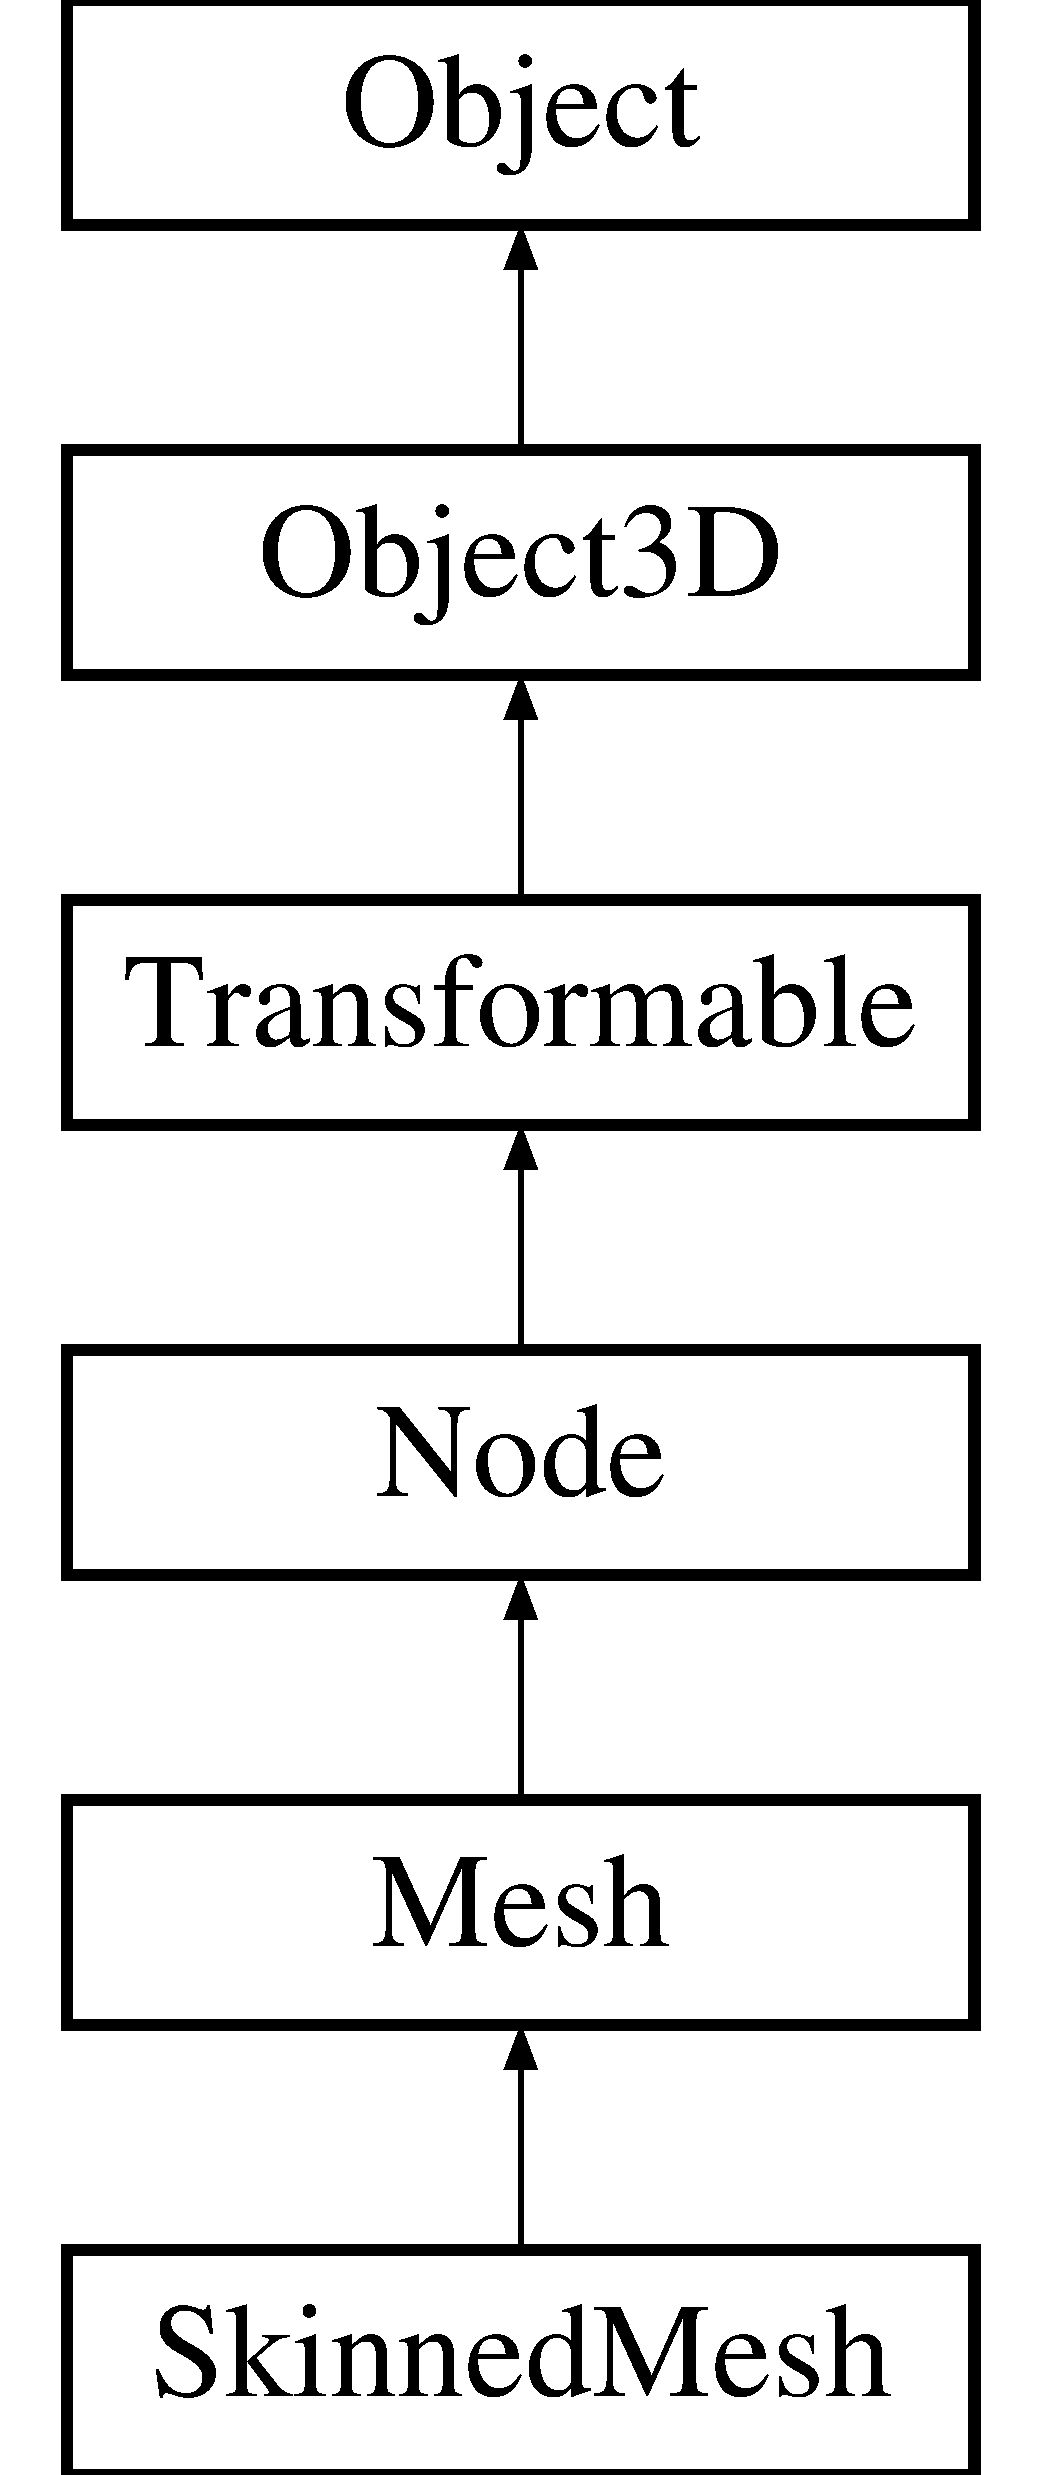
\includegraphics[height=6cm]{classm3g_1_1SkinnedMesh}
\end{center}
\end{figure}
\subsection*{Public Member Functions}
\begin{CompactItemize}
\item 
\hyperlink{classm3g_1_1SkinnedMesh_277419d6851b0e305f66a46095269915}{SkinnedMesh} (\hyperlink{classm3g_1_1VertexBuffer}{VertexBuffer} $\ast$vertices, int num\_\-submesh, \hyperlink{classm3g_1_1IndexBuffer}{IndexBuffer} $\ast$$\ast$submeshes, \hyperlink{classm3g_1_1Appearance}{Appearance} $\ast$$\ast$apperarances, Group $\ast$skeleton)
\item 
\hyperlink{classm3g_1_1SkinnedMesh_094bf88089897beeb8b8776e3bbb299d}{SkinnedMesh} (\hyperlink{classm3g_1_1VertexBuffer}{VertexBuffer} $\ast$vertices, \hyperlink{classm3g_1_1IndexBuffer}{IndexBuffer} $\ast$submeshes, \hyperlink{classm3g_1_1Appearance}{Appearance} $\ast$apperarances, Group $\ast$skeleton)
\item 
virtual \hyperlink{classm3g_1_1SkinnedMesh_c73da5b5c5f8f14fc241328b4b78928c}{$\sim$SkinnedMesh} ()
\item 
virtual \hyperlink{classm3g_1_1SkinnedMesh}{SkinnedMesh} $\ast$ \hyperlink{classm3g_1_1SkinnedMesh_d3f422cf7656b73687d789094c7eae42}{duplicate} () const 
\item 
virtual int \hyperlink{classm3g_1_1SkinnedMesh_8aad1ceab4c2a03609c8a42324ce484d}{animate} (int world\_\-time)
\item 
void \hyperlink{classm3g_1_1SkinnedMesh_05077c4ee16f87ed4163f4d7a5f4f735}{addTransform} (\hyperlink{classm3g_1_1Node}{Node} $\ast$bone, int weight, int first\_\-vertex, int num\_\-vertices)
\item 
void \hyperlink{classm3g_1_1SkinnedMesh_e6c2fed8109053ded845e49f5c3b0c73}{getBoneTransform} (\hyperlink{classm3g_1_1Node}{Node} $\ast$bone, \hyperlink{classm3g_1_1Transform}{Transform} $\ast$transform) const 
\item 
int \hyperlink{classm3g_1_1SkinnedMesh_84ec0935b92b7ccc0aed7e66c4eac78f}{getBoneVertices} (\hyperlink{classm3g_1_1Node}{Node} $\ast$bone, int $\ast$vertex\_\-indices, float $\ast$weights) const 
\item 
Group $\ast$ \hyperlink{classm3g_1_1SkinnedMesh_ce7d69c2b600f6f01a46214db28e6f92}{getSkeleton} () const 
\item 
virtual bool \hyperlink{classm3g_1_1SkinnedMesh_dc812d8230f94f0b6b8e4fecdb802a16}{intersect} (const \hyperlink{classm3g_1_1Vector}{Vector} \&org, const \hyperlink{classm3g_1_1Vector}{Vector} \&dir, \hyperlink{classm3g_1_1RayIntersection}{RayIntersection} $\ast$ri) const 
\item 
virtual std::ostream \& \hyperlink{classm3g_1_1SkinnedMesh_6fea17fa1532df3794f8cb39cb4f911f}{print} (std::ostream \&out) const 
\item 
virtual void \hyperlink{classm3g_1_1SkinnedMesh_8babc8a79b78615da51161e94029eea9}{render} (\hyperlink{structm3g_1_1RenderState}{RenderState} \&state) const 
\end{CompactItemize}


\subsection{Detailed Description}
A scene graph node that represents a skeletally animated polygon mesh. 

\subsection{Constructor \& Destructor Documentation}
\hypertarget{classm3g_1_1SkinnedMesh_277419d6851b0e305f66a46095269915}{
\index{m3g::SkinnedMesh@{m3g::SkinnedMesh}!SkinnedMesh@{SkinnedMesh}}
\index{SkinnedMesh@{SkinnedMesh}!m3g::SkinnedMesh@{m3g::SkinnedMesh}}
\subsubsection[{SkinnedMesh}]{\setlength{\rightskip}{0pt plus 5cm}{\bf SkinnedMesh} ({\bf VertexBuffer} $\ast$ {\em vertices}, \/  int {\em num\_\-submesh}, \/  {\bf IndexBuffer} $\ast$$\ast$ {\em submeshes}, \/  {\bf Appearance} $\ast$$\ast$ {\em appearances\_\-}, \/  Group $\ast$ {\em skeleton\_\-})}}
\label{classm3g_1_1SkinnedMesh_277419d6851b0e305f66a46095269915}


Constructs a new \hyperlink{classm3g_1_1SkinnedMesh}{SkinnedMesh} witdh the given vertices, submeshes and skeleton.

メモ:skeletonのparentをthisにするべき? それをすると現状では動かない。 \hypertarget{classm3g_1_1SkinnedMesh_094bf88089897beeb8b8776e3bbb299d}{
\index{m3g::SkinnedMesh@{m3g::SkinnedMesh}!SkinnedMesh@{SkinnedMesh}}
\index{SkinnedMesh@{SkinnedMesh}!m3g::SkinnedMesh@{m3g::SkinnedMesh}}
\subsubsection[{SkinnedMesh}]{\setlength{\rightskip}{0pt plus 5cm}{\bf SkinnedMesh} ({\bf VertexBuffer} $\ast$ {\em vertices}, \/  {\bf IndexBuffer} $\ast$ {\em submeshes}, \/  {\bf Appearance} $\ast$ {\em apperarances}, \/  Group $\ast$ {\em skeleton})}}
\label{classm3g_1_1SkinnedMesh_094bf88089897beeb8b8776e3bbb299d}


Constructs a new \hyperlink{classm3g_1_1SkinnedMesh}{SkinnedMesh} witdh the given vertices, submeshes and skeleton. \hypertarget{classm3g_1_1SkinnedMesh_c73da5b5c5f8f14fc241328b4b78928c}{
\index{m3g::SkinnedMesh@{m3g::SkinnedMesh}!$\sim$SkinnedMesh@{$\sim$SkinnedMesh}}
\index{$\sim$SkinnedMesh@{$\sim$SkinnedMesh}!m3g::SkinnedMesh@{m3g::SkinnedMesh}}
\subsubsection[{$\sim$SkinnedMesh}]{\setlength{\rightskip}{0pt plus 5cm}$\sim${\bf SkinnedMesh} ()\hspace{0.3cm}{\tt  \mbox{[}virtual\mbox{]}}}}
\label{classm3g_1_1SkinnedMesh_c73da5b5c5f8f14fc241328b4b78928c}


Destructs this object. 

\subsection{Member Function Documentation}
\hypertarget{classm3g_1_1SkinnedMesh_05077c4ee16f87ed4163f4d7a5f4f735}{
\index{m3g::SkinnedMesh@{m3g::SkinnedMesh}!addTransform@{addTransform}}
\index{addTransform@{addTransform}!m3g::SkinnedMesh@{m3g::SkinnedMesh}}
\subsubsection[{addTransform}]{\setlength{\rightskip}{0pt plus 5cm}void addTransform ({\bf Node} $\ast$ {\em bone}, \/  int {\em weight}, \/  int {\em first\_\-vertex}, \/  int {\em num\_\-vertices})}}
\label{classm3g_1_1SkinnedMesh_05077c4ee16f87ed4163f4d7a5f4f735}


Associates a weighted transformation, or \char`\"{}bone\char`\"{}, with a range of vertices int this \hyperlink{classm3g_1_1SkinnedMesh}{SkinnedMesh}. \hypertarget{classm3g_1_1SkinnedMesh_8aad1ceab4c2a03609c8a42324ce484d}{
\index{m3g::SkinnedMesh@{m3g::SkinnedMesh}!animate@{animate}}
\index{animate@{animate}!m3g::SkinnedMesh@{m3g::SkinnedMesh}}
\subsubsection[{animate}]{\setlength{\rightskip}{0pt plus 5cm}int animate (int {\em world\_\-time})\hspace{0.3cm}{\tt  \mbox{[}virtual\mbox{]}}}}
\label{classm3g_1_1SkinnedMesh_8aad1ceab4c2a03609c8a42324ce484d}


Updates all animated properties in this \hyperlink{classm3g_1_1Object3D}{Object3D} and all Object3Ds that are reachable from this \hyperlink{classm3g_1_1Object3D}{Object3D}. 

Reimplemented from \hyperlink{classm3g_1_1Mesh_8aad1ceab4c2a03609c8a42324ce484d}{Mesh}.\hypertarget{classm3g_1_1SkinnedMesh_d3f422cf7656b73687d789094c7eae42}{
\index{m3g::SkinnedMesh@{m3g::SkinnedMesh}!duplicate@{duplicate}}
\index{duplicate@{duplicate}!m3g::SkinnedMesh@{m3g::SkinnedMesh}}
\subsubsection[{duplicate}]{\setlength{\rightskip}{0pt plus 5cm}{\bf SkinnedMesh} $\ast$ duplicate () const\hspace{0.3cm}{\tt  \mbox{[}virtual\mbox{]}}}}
\label{classm3g_1_1SkinnedMesh_d3f422cf7656b73687d789094c7eae42}


Creates a duplicate of this \hyperlink{classm3g_1_1Object3D}{Object3D}. 

Reimplemented from \hyperlink{classm3g_1_1Mesh_52ce6d0b3eda2bd3a95bfb5b7dbb6f82}{Mesh}.\hypertarget{classm3g_1_1SkinnedMesh_e6c2fed8109053ded845e49f5c3b0c73}{
\index{m3g::SkinnedMesh@{m3g::SkinnedMesh}!getBoneTransform@{getBoneTransform}}
\index{getBoneTransform@{getBoneTransform}!m3g::SkinnedMesh@{m3g::SkinnedMesh}}
\subsubsection[{getBoneTransform}]{\setlength{\rightskip}{0pt plus 5cm}void getBoneTransform ({\bf Node} $\ast$ {\em bone}, \/  {\bf Transform} $\ast$ {\em transform}) const}}
\label{classm3g_1_1SkinnedMesh_e6c2fed8109053ded845e49f5c3b0c73}


Returns the at-rest tarnsformation (from local coordinate to bone coordinate) for a bone node. \hypertarget{classm3g_1_1SkinnedMesh_84ec0935b92b7ccc0aed7e66c4eac78f}{
\index{m3g::SkinnedMesh@{m3g::SkinnedMesh}!getBoneVertices@{getBoneVertices}}
\index{getBoneVertices@{getBoneVertices}!m3g::SkinnedMesh@{m3g::SkinnedMesh}}
\subsubsection[{getBoneVertices}]{\setlength{\rightskip}{0pt plus 5cm}int getBoneVertices ({\bf Node} $\ast$ {\em bone}, \/  int $\ast$ {\em vertex\_\-indices}, \/  float $\ast$ {\em weights}) const}}
\label{classm3g_1_1SkinnedMesh_84ec0935b92b7ccc0aed7e66c4eac78f}


Returns the number of vertices influenced by the given bone, filling in the vertices and their weights to given arrays. \hypertarget{classm3g_1_1SkinnedMesh_ce7d69c2b600f6f01a46214db28e6f92}{
\index{m3g::SkinnedMesh@{m3g::SkinnedMesh}!getSkeleton@{getSkeleton}}
\index{getSkeleton@{getSkeleton}!m3g::SkinnedMesh@{m3g::SkinnedMesh}}
\subsubsection[{getSkeleton}]{\setlength{\rightskip}{0pt plus 5cm}Group $\ast$ getSkeleton () const}}
\label{classm3g_1_1SkinnedMesh_ce7d69c2b600f6f01a46214db28e6f92}


Returns the skeleton Group of this \hyperlink{classm3g_1_1SkinnedMesh}{SkinnedMesh}. \hypertarget{classm3g_1_1SkinnedMesh_dc812d8230f94f0b6b8e4fecdb802a16}{
\index{m3g::SkinnedMesh@{m3g::SkinnedMesh}!intersect@{intersect}}
\index{intersect@{intersect}!m3g::SkinnedMesh@{m3g::SkinnedMesh}}
\subsubsection[{intersect}]{\setlength{\rightskip}{0pt plus 5cm}bool intersect (const {\bf Vector} \& {\em org}, \/  const {\bf Vector} \& {\em dir}, \/  {\bf RayIntersection} $\ast$ {\em ri}) const\hspace{0.3cm}{\tt  \mbox{[}virtual\mbox{]}}}}
\label{classm3g_1_1SkinnedMesh_dc812d8230f94f0b6b8e4fecdb802a16}


座標は全てこのメッシュのローカル座標系で指定する. 

Reimplemented from \hyperlink{classm3g_1_1Mesh_dc812d8230f94f0b6b8e4fecdb802a16}{Mesh}.\hypertarget{classm3g_1_1SkinnedMesh_6fea17fa1532df3794f8cb39cb4f911f}{
\index{m3g::SkinnedMesh@{m3g::SkinnedMesh}!print@{print}}
\index{print@{print}!m3g::SkinnedMesh@{m3g::SkinnedMesh}}
\subsubsection[{print}]{\setlength{\rightskip}{0pt plus 5cm}std::ostream \& print (std::ostream \& {\em out}) const\hspace{0.3cm}{\tt  \mbox{[}virtual\mbox{]}}}}
\label{classm3g_1_1SkinnedMesh_6fea17fa1532df3794f8cb39cb4f911f}


Print out information of this class, for debug only. 

Reimplemented from \hyperlink{classm3g_1_1Mesh_6fea17fa1532df3794f8cb39cb4f911f}{Mesh}.\hypertarget{classm3g_1_1SkinnedMesh_8babc8a79b78615da51161e94029eea9}{
\index{m3g::SkinnedMesh@{m3g::SkinnedMesh}!render@{render}}
\index{render@{render}!m3g::SkinnedMesh@{m3g::SkinnedMesh}}
\subsubsection[{render}]{\setlength{\rightskip}{0pt plus 5cm}void render ({\bf RenderState} \& {\em state}) const\hspace{0.3cm}{\tt  \mbox{[}virtual\mbox{]}}}}
\label{classm3g_1_1SkinnedMesh_8babc8a79b78615da51161e94029eea9}


Render this object.

Note: \hyperlink{classm3g_1_1Mesh}{Mesh} should be rendered only at second rendering pass(pass=2). In other cases, do nothing. 

Reimplemented from \hyperlink{classm3g_1_1Mesh_8babc8a79b78615da51161e94029eea9}{Mesh}.

The documentation for this class was generated from the following files:\begin{CompactItemize}
\item 
/work/workspace.desktop-m3g/src/SkinnedMesh.hpp\item 
/work/workspace.desktop-m3g/src/SkinnedMesh.cpp\end{CompactItemize}

\hypertarget{classm3g_1_1Sprite3D}{
\section{クラス Sprite3D}
\label{classm3g_1_1Sprite3D}\index{m3g::Sprite3D@{m3g::Sprite3D}}
}
{\tt \#include $<$Sprite3D.hpp$>$}

Sprite3Dに対する継承グラフ:\begin{figure}[H]
\begin{center}
\leavevmode
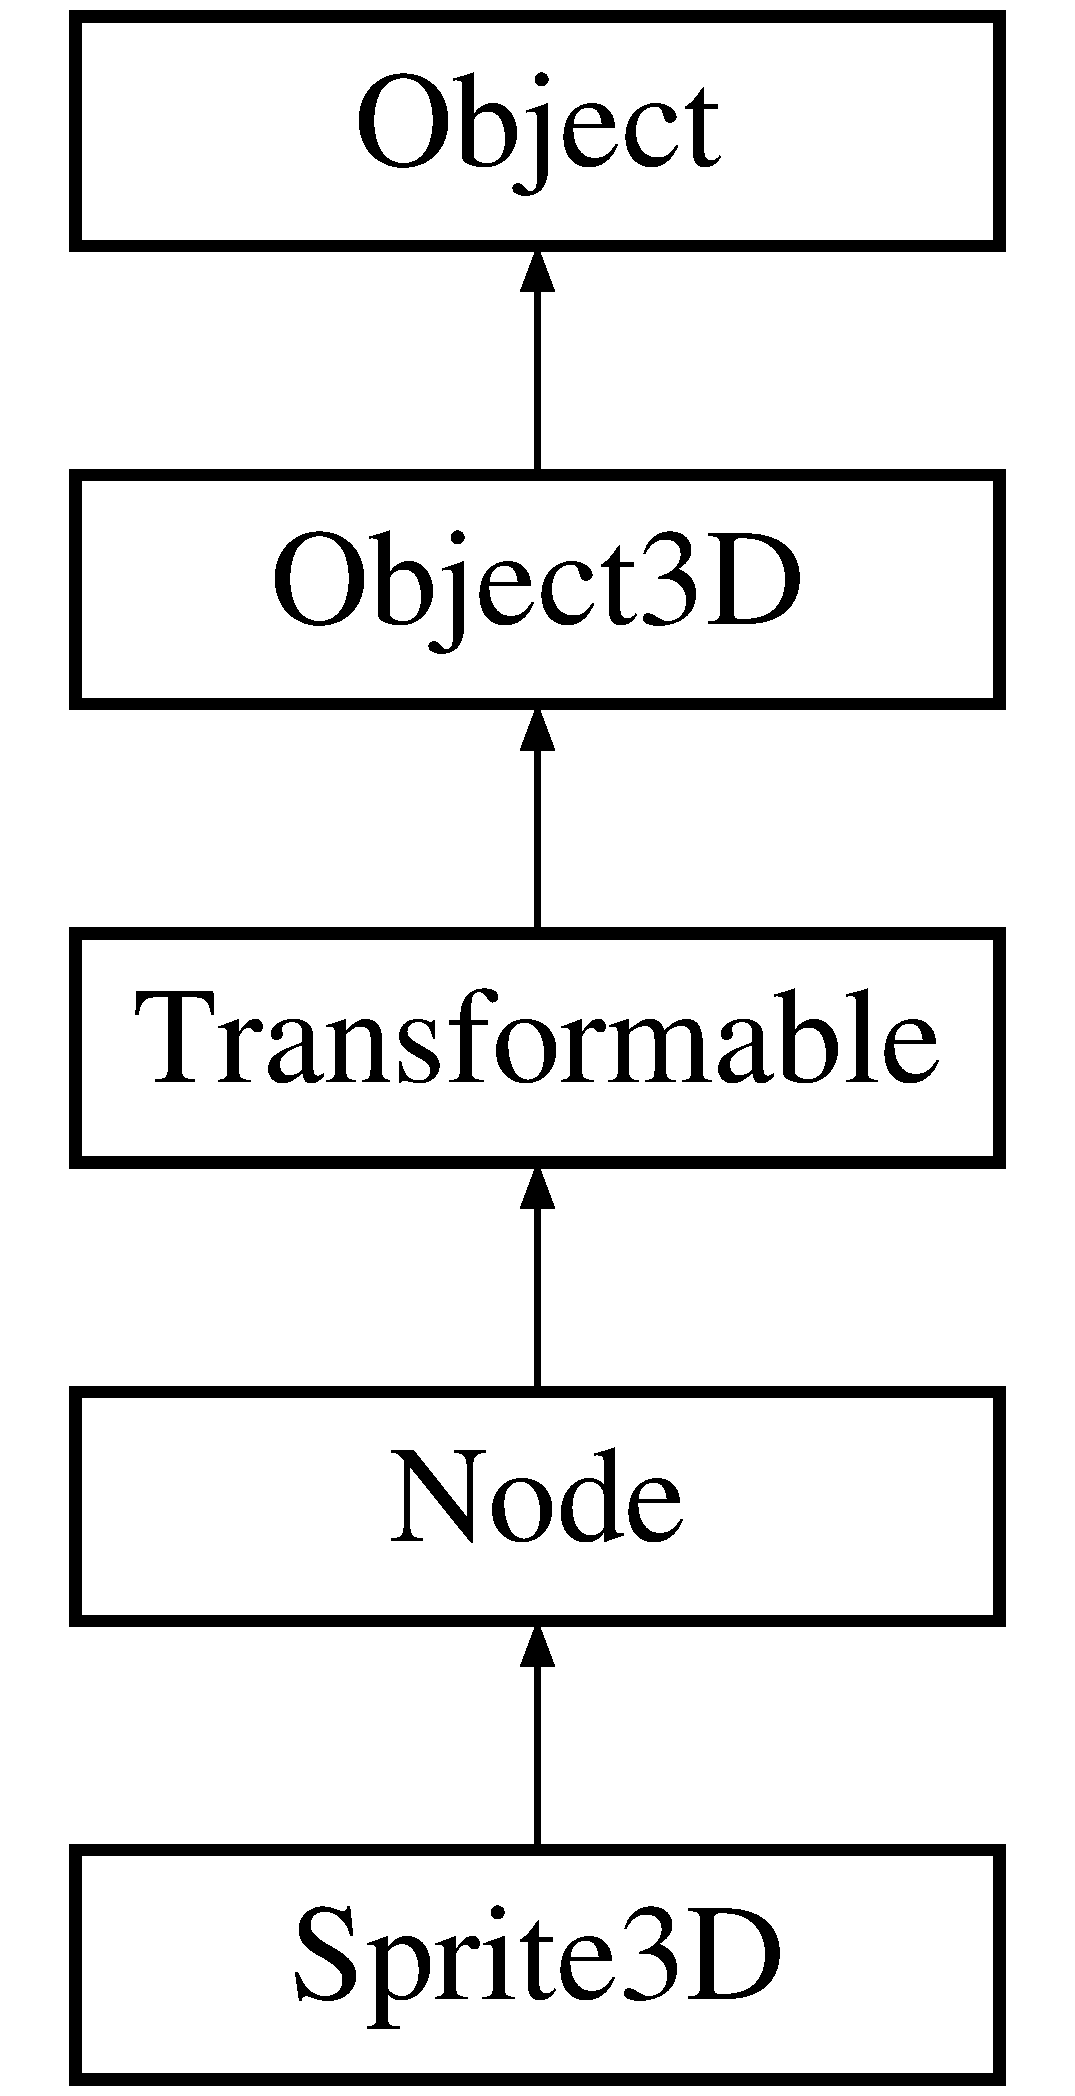
\includegraphics[height=5cm]{classm3g_1_1Sprite3D}
\end{center}
\end{figure}
\subsection*{構成}
\begin{CompactItemize}
\item 
struct \hyperlink{structm3g_1_1Sprite3D_1_1CropRect}{CropRect}
\end{CompactItemize}
\subsection*{Public メソッド}
\begin{CompactItemize}
\item 
\hyperlink{classm3g_1_1Sprite3D_9cb33fd453d441ed8e99b95f5e29df0c}{Sprite3D} (bool scaled, \hyperlink{classm3g_1_1Image2D}{Image2D} $\ast$image, \hyperlink{classm3g_1_1Appearance}{Appearance} $\ast$appearance)
\item 
virtual \hyperlink{classm3g_1_1Sprite3D_a57bd1e3141ba11c88ddec1e46c188d6}{$\sim$Sprite3D} ()
\item 
\hyperlink{classm3g_1_1Sprite3D}{Sprite3D} $\ast$ \hyperlink{classm3g_1_1Sprite3D_0af34e87be803eb476f9e118d2363246}{duplicate} () const 
\item 
virtual void \hyperlink{classm3g_1_1Sprite3D_415c0b110f95410ded9b85e5d99a496b}{addAnimationTrack} (\hyperlink{classm3g_1_1AnimationTrack}{AnimationTrack} $\ast$animation\_\-track)
\item 
virtual int \hyperlink{classm3g_1_1Sprite3D_8aad1ceab4c2a03609c8a42324ce484d}{animate} (int world\_\-time)
\item 
\hyperlink{classm3g_1_1Appearance}{Appearance} $\ast$ \hyperlink{classm3g_1_1Sprite3D_0219cb20ddea978a5796b5b414d012d2}{getAppearance} () const 
\item 
int \hyperlink{classm3g_1_1Sprite3D_d6d9d6f23b7bb004c93642bcd081f4a3}{getCropHeight} () const 
\item 
int \hyperlink{classm3g_1_1Sprite3D_5c6515f6706675ef31ca5dfa0a03b953}{getCropWidth} () const 
\item 
int \hyperlink{classm3g_1_1Sprite3D_d0ba0211183decc8f0459ca598b12912}{getCropX} () const 
\item 
int \hyperlink{classm3g_1_1Sprite3D_9ef03b219415a1f08aef6745ad5d87d0}{getCropY} () const 
\item 
\hyperlink{classm3g_1_1Image2D}{Image2D} $\ast$ \hyperlink{classm3g_1_1Sprite3D_a8c0193b0e7d47d4b5c9f60df24c44f5}{getImage} () const 
\item 
bool \hyperlink{classm3g_1_1Sprite3D_8e3e7fa70e1d3f2342580991105779f5}{isScaled} () const 
\item 
void \hyperlink{classm3g_1_1Sprite3D_b9b44bad4241635062ed66437c9bae48}{setAppearance} (\hyperlink{classm3g_1_1Appearance}{Appearance} $\ast$appearance)
\item 
void \hyperlink{classm3g_1_1Sprite3D_35ca6d3ff64f2232a0f3a11bf4ab483e}{setCrop} (int crop\_\-x, int crop\_\-y, int width, int height)
\item 
void \hyperlink{classm3g_1_1Sprite3D_705b89b41cd1b38f664ed912be44baaa}{setImage} (\hyperlink{classm3g_1_1Image2D}{Image2D} $\ast$image)
\item 
virtual std::ostream \& \hyperlink{classm3g_1_1Sprite3D_6fea17fa1532df3794f8cb39cb4f911f}{print} (std::ostream \&out) const 
\end{CompactItemize}
\subsection*{Protected メソッド}
\begin{CompactItemize}
\item 
virtual void \hyperlink{classm3g_1_1Sprite3D_8babc8a79b78615da51161e94029eea9}{render} (\hyperlink{structm3g_1_1RenderState}{RenderState} \&state) const 
\end{CompactItemize}
\subsection*{フレンド}
\begin{CompactItemize}
\item 
\hypertarget{classm3g_1_1Sprite3D_2697825715974a353728f0d4d5658112}{
class \textbf{Group}}
\label{classm3g_1_1Sprite3D_2697825715974a353728f0d4d5658112}

\end{CompactItemize}


\subsection{説明}
3Dの位置情報を持った2D画像を表すシーングラフノード. 

\subsection{コンストラクタとデストラクタ}
\hypertarget{classm3g_1_1Sprite3D_9cb33fd453d441ed8e99b95f5e29df0c}{
\index{m3g::Sprite3D@{m3g::Sprite3D}!Sprite3D@{Sprite3D}}
\index{Sprite3D@{Sprite3D}!m3g::Sprite3D@{m3g::Sprite3D}}
\subsubsection[{Sprite3D}]{\setlength{\rightskip}{0pt plus 5cm}{\bf Sprite3D} (bool {\em scaled}, \/  {\bf Image2D} $\ast$ {\em image}, \/  {\bf Appearance} $\ast$ {\em appearance})}}
\label{classm3g_1_1Sprite3D_9cb33fd453d441ed8e99b95f5e29df0c}


指定されたスケーリングモード、画像、アピアランスを持ったSprite3Dの作成. \hypertarget{classm3g_1_1Sprite3D_a57bd1e3141ba11c88ddec1e46c188d6}{
\index{m3g::Sprite3D@{m3g::Sprite3D}!$\sim$Sprite3D@{$\sim$Sprite3D}}
\index{$\sim$Sprite3D@{$\sim$Sprite3D}!m3g::Sprite3D@{m3g::Sprite3D}}
\subsubsection[{$\sim$Sprite3D}]{\setlength{\rightskip}{0pt plus 5cm}$\sim${\bf Sprite3D} ()\hspace{0.3cm}{\tt  \mbox{[}virtual\mbox{]}}}}
\label{classm3g_1_1Sprite3D_a57bd1e3141ba11c88ddec1e46c188d6}


このオブジェクトを削除するデストラクタ. 

\subsection{関数}
\hypertarget{classm3g_1_1Sprite3D_415c0b110f95410ded9b85e5d99a496b}{
\index{m3g::Sprite3D@{m3g::Sprite3D}!addAnimationTrack@{addAnimationTrack}}
\index{addAnimationTrack@{addAnimationTrack}!m3g::Sprite3D@{m3g::Sprite3D}}
\subsubsection[{addAnimationTrack}]{\setlength{\rightskip}{0pt plus 5cm}void addAnimationTrack ({\bf AnimationTrack} $\ast$ {\em animation\_\-track})\hspace{0.3cm}{\tt  \mbox{[}virtual\mbox{]}}}}
\label{classm3g_1_1Sprite3D_415c0b110f95410ded9b85e5d99a496b}


このObject3Dに指定されたアニメーショントラックを追加する。 既存のトラックの順番とインデックスは変更されるかもしれない. 

\hyperlink{classm3g_1_1Node_415c0b110f95410ded9b85e5d99a496b}{Node}を再定義しています。\hypertarget{classm3g_1_1Sprite3D_8aad1ceab4c2a03609c8a42324ce484d}{
\index{m3g::Sprite3D@{m3g::Sprite3D}!animate@{animate}}
\index{animate@{animate}!m3g::Sprite3D@{m3g::Sprite3D}}
\subsubsection[{animate}]{\setlength{\rightskip}{0pt plus 5cm}int animate (int {\em world\_\-time})\hspace{0.3cm}{\tt  \mbox{[}virtual\mbox{]}}}}
\label{classm3g_1_1Sprite3D_8aad1ceab4c2a03609c8a42324ce484d}


このObject3D自身とここから到達できるObject3Dのアニメーテッドプロパティを更新する. 

\hyperlink{classm3g_1_1Node_8aad1ceab4c2a03609c8a42324ce484d}{Node}を再定義しています。\hypertarget{classm3g_1_1Sprite3D_0af34e87be803eb476f9e118d2363246}{
\index{m3g::Sprite3D@{m3g::Sprite3D}!duplicate@{duplicate}}
\index{duplicate@{duplicate}!m3g::Sprite3D@{m3g::Sprite3D}}
\subsubsection[{duplicate}]{\setlength{\rightskip}{0pt plus 5cm}{\bf Sprite3D} $\ast$ duplicate () const\hspace{0.3cm}{\tt  \mbox{[}virtual\mbox{]}}}}
\label{classm3g_1_1Sprite3D_0af34e87be803eb476f9e118d2363246}


このオブジェクトの複製の作成. 

\hyperlink{classm3g_1_1Node_0b9f7531a4b56d34f47aeb1fff0d37e0}{Node}を再定義しています。\hypertarget{classm3g_1_1Sprite3D_0219cb20ddea978a5796b5b414d012d2}{
\index{m3g::Sprite3D@{m3g::Sprite3D}!getAppearance@{getAppearance}}
\index{getAppearance@{getAppearance}!m3g::Sprite3D@{m3g::Sprite3D}}
\subsubsection[{getAppearance}]{\setlength{\rightskip}{0pt plus 5cm}{\bf Appearance} $\ast$ getAppearance () const}}
\label{classm3g_1_1Sprite3D_0219cb20ddea978a5796b5b414d012d2}


このSprite3Dのカレントのアピアランスを取得. \hypertarget{classm3g_1_1Sprite3D_d6d9d6f23b7bb004c93642bcd081f4a3}{
\index{m3g::Sprite3D@{m3g::Sprite3D}!getCropHeight@{getCropHeight}}
\index{getCropHeight@{getCropHeight}!m3g::Sprite3D@{m3g::Sprite3D}}
\subsubsection[{getCropHeight}]{\setlength{\rightskip}{0pt plus 5cm}int getCropHeight () const}}
\label{classm3g_1_1Sprite3D_d6d9d6f23b7bb004c93642bcd081f4a3}


ソース画像のカレントのクロップ領域の高さの取得. \hypertarget{classm3g_1_1Sprite3D_5c6515f6706675ef31ca5dfa0a03b953}{
\index{m3g::Sprite3D@{m3g::Sprite3D}!getCropWidth@{getCropWidth}}
\index{getCropWidth@{getCropWidth}!m3g::Sprite3D@{m3g::Sprite3D}}
\subsubsection[{getCropWidth}]{\setlength{\rightskip}{0pt plus 5cm}int getCropWidth () const}}
\label{classm3g_1_1Sprite3D_5c6515f6706675ef31ca5dfa0a03b953}


ソース画像のカレントのクロップ領域の高さの取得. \hypertarget{classm3g_1_1Sprite3D_d0ba0211183decc8f0459ca598b12912}{
\index{m3g::Sprite3D@{m3g::Sprite3D}!getCropX@{getCropX}}
\index{getCropX@{getCropX}!m3g::Sprite3D@{m3g::Sprite3D}}
\subsubsection[{getCropX}]{\setlength{\rightskip}{0pt plus 5cm}int getCropX () const}}
\label{classm3g_1_1Sprite3D_d0ba0211183decc8f0459ca598b12912}


クロップ矩形のソース画像の左上からのX方向の相対オフセット. \hypertarget{classm3g_1_1Sprite3D_9ef03b219415a1f08aef6745ad5d87d0}{
\index{m3g::Sprite3D@{m3g::Sprite3D}!getCropY@{getCropY}}
\index{getCropY@{getCropY}!m3g::Sprite3D@{m3g::Sprite3D}}
\subsubsection[{getCropY}]{\setlength{\rightskip}{0pt plus 5cm}int getCropY () const}}
\label{classm3g_1_1Sprite3D_9ef03b219415a1f08aef6745ad5d87d0}


クロップ矩形のソース画像の左上からのY方向の相対オフセット. \hypertarget{classm3g_1_1Sprite3D_a8c0193b0e7d47d4b5c9f60df24c44f5}{
\index{m3g::Sprite3D@{m3g::Sprite3D}!getImage@{getImage}}
\index{getImage@{getImage}!m3g::Sprite3D@{m3g::Sprite3D}}
\subsubsection[{getImage}]{\setlength{\rightskip}{0pt plus 5cm}{\bf Image2D} $\ast$ getImage () const}}
\label{classm3g_1_1Sprite3D_a8c0193b0e7d47d4b5c9f60df24c44f5}


カレントのSprite3D画像の取得. \hypertarget{classm3g_1_1Sprite3D_8e3e7fa70e1d3f2342580991105779f5}{
\index{m3g::Sprite3D@{m3g::Sprite3D}!isScaled@{isScaled}}
\index{isScaled@{isScaled}!m3g::Sprite3D@{m3g::Sprite3D}}
\subsubsection[{isScaled}]{\setlength{\rightskip}{0pt plus 5cm}bool isScaled () const}}
\label{classm3g_1_1Sprite3D_8e3e7fa70e1d3f2342580991105779f5}


このSprite3Dの自動スケーリングの状態を返す. \hypertarget{classm3g_1_1Sprite3D_6fea17fa1532df3794f8cb39cb4f911f}{
\index{m3g::Sprite3D@{m3g::Sprite3D}!print@{print}}
\index{print@{print}!m3g::Sprite3D@{m3g::Sprite3D}}
\subsubsection[{print}]{\setlength{\rightskip}{0pt plus 5cm}std::ostream \& print (std::ostream \& {\em out}) const\hspace{0.3cm}{\tt  \mbox{[}virtual\mbox{]}}}}
\label{classm3g_1_1Sprite3D_6fea17fa1532df3794f8cb39cb4f911f}


このSprite3Dクラスの情報を表示する。デバッグ用. 

\hyperlink{classm3g_1_1Node_6fea17fa1532df3794f8cb39cb4f911f}{Node}を再定義しています。\hypertarget{classm3g_1_1Sprite3D_8babc8a79b78615da51161e94029eea9}{
\index{m3g::Sprite3D@{m3g::Sprite3D}!render@{render}}
\index{render@{render}!m3g::Sprite3D@{m3g::Sprite3D}}
\subsubsection[{render}]{\setlength{\rightskip}{0pt plus 5cm}void render ({\bf RenderState} \& {\em state}) const\hspace{0.3cm}{\tt  \mbox{[}protected, virtual\mbox{]}}}}
\label{classm3g_1_1Sprite3D_8babc8a79b78615da51161e94029eea9}


このノードをレンダリングする内部使用の関数.

Note: \hyperlink{classm3g_1_1Sprite3D}{Sprite3D} should be rendered only at second rendering pass(pass=2). In other cases, do nothing. メモ: 改良の余地があるな……。あとappearanceがNULLの時は”何もしない”ではなく ”デフォルトでレンダー”にすべき。 

\hyperlink{classm3g_1_1Node_8babc8a79b78615da51161e94029eea9}{Node}を再定義しています。\hypertarget{classm3g_1_1Sprite3D_b9b44bad4241635062ed66437c9bae48}{
\index{m3g::Sprite3D@{m3g::Sprite3D}!setAppearance@{setAppearance}}
\index{setAppearance@{setAppearance}!m3g::Sprite3D@{m3g::Sprite3D}}
\subsubsection[{setAppearance}]{\setlength{\rightskip}{0pt plus 5cm}void setAppearance ({\bf Appearance} $\ast$ {\em appearance})}}
\label{classm3g_1_1Sprite3D_b9b44bad4241635062ed66437c9bae48}


このSprite3Dのアピアランスの設定. \hypertarget{classm3g_1_1Sprite3D_35ca6d3ff64f2232a0f3a11bf4ab483e}{
\index{m3g::Sprite3D@{m3g::Sprite3D}!setCrop@{setCrop}}
\index{setCrop@{setCrop}!m3g::Sprite3D@{m3g::Sprite3D}}
\subsubsection[{setCrop}]{\setlength{\rightskip}{0pt plus 5cm}void setCrop (int {\em crop\_\-x}, \/  int {\em crop\_\-y}, \/  int {\em width}, \/  int {\em height})}}
\label{classm3g_1_1Sprite3D_35ca6d3ff64f2232a0f3a11bf4ab483e}


ソース画像のクロッピング矩形の設定. \hypertarget{classm3g_1_1Sprite3D_705b89b41cd1b38f664ed912be44baaa}{
\index{m3g::Sprite3D@{m3g::Sprite3D}!setImage@{setImage}}
\index{setImage@{setImage}!m3g::Sprite3D@{m3g::Sprite3D}}
\subsubsection[{setImage}]{\setlength{\rightskip}{0pt plus 5cm}void setImage ({\bf Image2D} $\ast$ {\em image})}}
\label{classm3g_1_1Sprite3D_705b89b41cd1b38f664ed912be44baaa}


表示するスプライト画像の設定. 

このクラスの説明は次のファイルから生成されました:\begin{CompactItemize}
\item 
/work/workspace.desktop-m3g/src/Sprite3D.hpp\item 
/work/workspace.desktop-m3g/src/Sprite3D.cpp\end{CompactItemize}

\hypertarget{classm3g_1_1Texture2D}{
\section{クラス Texture2D}
\label{classm3g_1_1Texture2D}\index{m3g::Texture2D@{m3g::Texture2D}}
}
{\tt \#include $<$Texture2D.hpp$>$}

Texture2Dに対する継承グラフ:\begin{figure}[H]
\begin{center}
\leavevmode
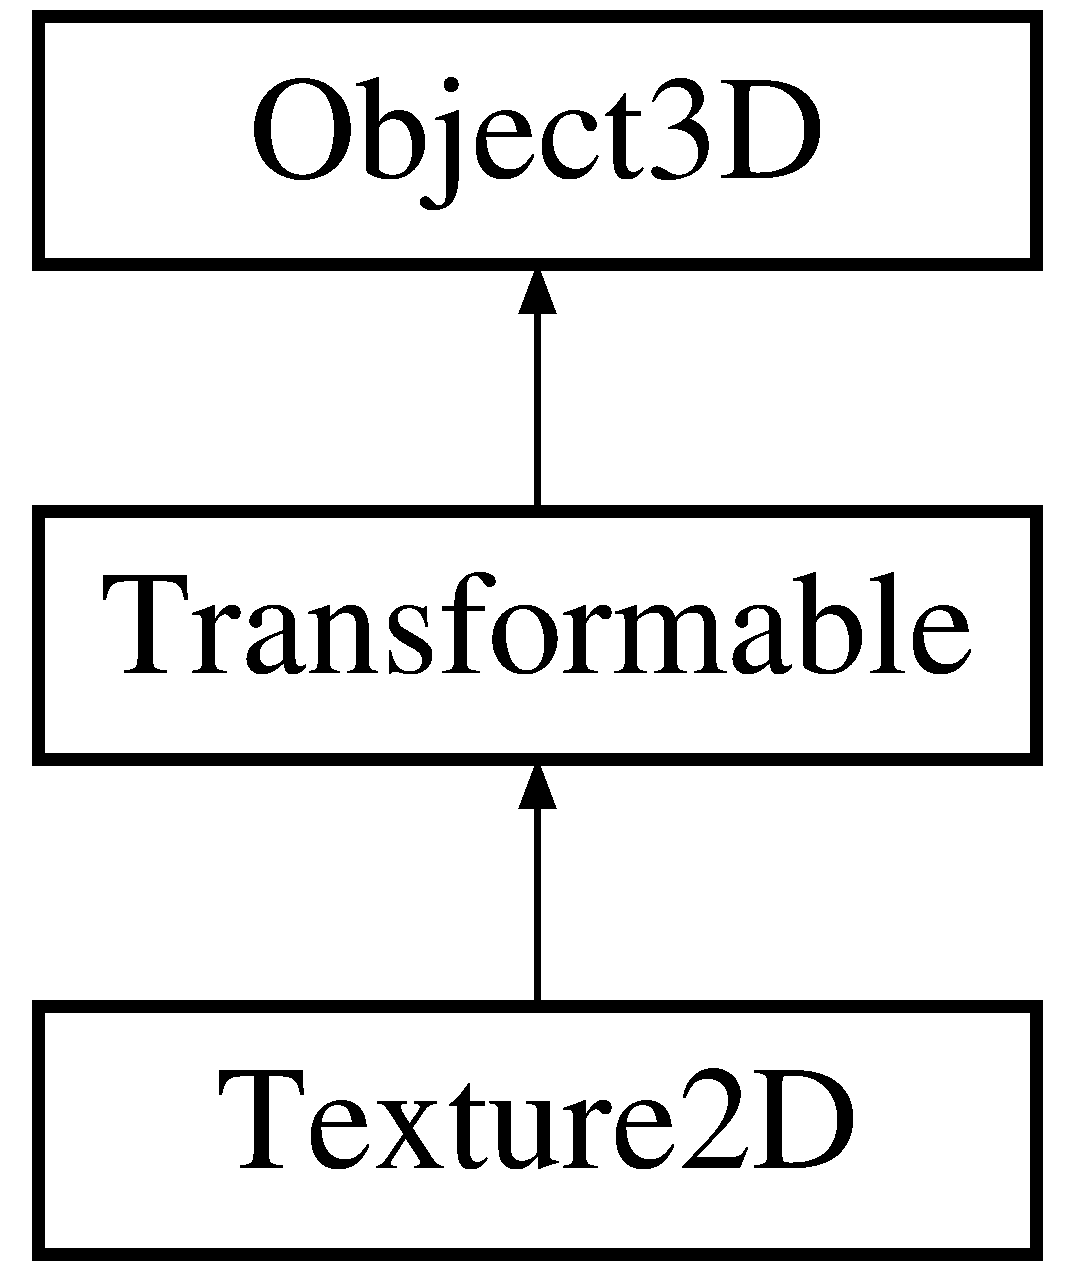
\includegraphics[height=4cm]{classm3g_1_1Texture2D}
\end{center}
\end{figure}
\subsection*{構成}
\begin{CompactItemize}
\item 
struct \textbf{Filter}
\item 
struct \textbf{Wrapping}
\end{CompactItemize}
\subsection*{Public メソッド}
\begin{CompactItemize}
\item 
\hyperlink{classm3g_1_1Texture2D_7a8d6431e41022e29ac936afc5e97b8e}{Texture2D} (\hyperlink{classm3g_1_1Image2D}{Image2D} $\ast$image)
\item 
virtual \hyperlink{classm3g_1_1Texture2D_060332aea614a81a914cd2e55f1794df}{$\sim$Texture2D} ()
\item 
\hyperlink{classm3g_1_1Texture2D}{Texture2D} $\ast$ \hyperlink{classm3g_1_1Texture2D_f4b50abcea8e4a6d6981c779d5009c05}{duplicate} () const 
\item 
virtual int \hyperlink{classm3g_1_1Texture2D_8aad1ceab4c2a03609c8a42324ce484d}{animate} (int world\_\-time)
\item 
virtual void \hyperlink{classm3g_1_1Texture2D_415c0b110f95410ded9b85e5d99a496b}{addAnimationTrack} (\hyperlink{classm3g_1_1AnimationTrack}{AnimationTrack} $\ast$animation\_\-track)
\item 
int \hyperlink{classm3g_1_1Texture2D_b7dc7b7bf2934448281894f2c1ef3638}{getBlendColor} () const 
\item 
int \hyperlink{classm3g_1_1Texture2D_078954de3d786bd11dc98b06f237bbbb}{getBlending} () const 
\item 
\hyperlink{classm3g_1_1Image2D}{Image2D} $\ast$ \hyperlink{classm3g_1_1Texture2D_a8c0193b0e7d47d4b5c9f60df24c44f5}{getImage} () const 
\item 
int \hyperlink{classm3g_1_1Texture2D_7b1e1ea0acc3d2096d346afdecc2ea5f}{getImageFilter} () const 
\item 
int \hyperlink{classm3g_1_1Texture2D_039f7813e846bedec1aaf4c413c15924}{getLevelFilter} () const 
\item 
int \hyperlink{classm3g_1_1Texture2D_6bdb583791178dc5002f4d0ae88293a9}{getWrappingS} () const 
\item 
int \hyperlink{classm3g_1_1Texture2D_58375e5e8ddde63dcf74f882d053ae3f}{getWrappingT} () const 
\item 
void \hyperlink{classm3g_1_1Texture2D_b5a6333203f443fb1f66ea2e39d4de1b}{setBlendColor} (int rgb)
\item 
void \hyperlink{classm3g_1_1Texture2D_189d98ce3e8ac7590be771944b3186d4}{setBlending} (int func)
\item 
void \hyperlink{classm3g_1_1Texture2D_857574b5c0f3e0ca9239bafb4008cae1}{setFiltering} (int level\_\-filter, int image\_\-filter)
\item 
void \hyperlink{classm3g_1_1Texture2D_705b89b41cd1b38f664ed912be44baaa}{setImage} (\hyperlink{classm3g_1_1Image2D}{Image2D} $\ast$image)
\item 
void \hyperlink{classm3g_1_1Texture2D_e676f34bd2f5ee1508ad1cb771702d8f}{setWrapping} (int wrap\_\-s, int wrap\_\-t)
\item 
virtual std::ostream \& \hyperlink{classm3g_1_1Texture2D_6fea17fa1532df3794f8cb39cb4f911f}{print} (std::ostream \&out) const 
\item 
virtual void \hyperlink{classm3g_1_1Texture2D_8babc8a79b78615da51161e94029eea9}{render} (\hyperlink{structm3g_1_1RenderState}{RenderState} \&state) const 
\end{CompactItemize}
\subsection*{Static Public 変数}
\begin{CompactItemize}
\item 
static const int \hyperlink{classm3g_1_1Texture2D_d1924d32385b5353ad11ecd8b1ec0ad5}{FILTER\_\-BASE\_\-LEVEL} = 208
\item 
static const int \hyperlink{classm3g_1_1Texture2D_5f06003f50141919a3665d22f55602a8}{FILTER\_\-LINEAR} = 209
\item 
static const int \hyperlink{classm3g_1_1Texture2D_1ee2e06d6462fdafd5f17e63eddfb8fe}{FILTER\_\-NEAREST} = 210
\item 
static const int \hyperlink{classm3g_1_1Texture2D_825ea3aff59f79958257ac557c802760}{FUNC\_\-ADD} = 224
\item 
static const int \hyperlink{classm3g_1_1Texture2D_57e3e01014bbfd62b8665586fdd2ecb3}{FUNC\_\-BLEND} = 225
\item 
static const int \hyperlink{classm3g_1_1Texture2D_235b942b18219513ca4a5a8c1a3171ac}{FUNC\_\-DECAL} = 226
\item 
static const int \hyperlink{classm3g_1_1Texture2D_4482b0d4d6d1f64aaf33c3c5862de30e}{FUNC\_\-MODULATE} = 227
\item 
static const int \hyperlink{classm3g_1_1Texture2D_14f24332e168c5e210ddad47fb5cdd17}{FUNC\_\-REPLACE} = 228
\item 
static const int \hyperlink{classm3g_1_1Texture2D_e36d8facf5b60eb6c59888121731c438}{WRAP\_\-CLAMP} = 240
\item 
static const int \hyperlink{classm3g_1_1Texture2D_b37ff061b9fb272284c4c389deec9266}{WRAP\_\-REPEAT} = 241
\end{CompactItemize}
\subsection*{フレンド}
\begin{CompactItemize}
\item 
\hypertarget{classm3g_1_1Texture2D_afa5201a494f65c37039281d9b63a2a9}{
class \textbf{Appearance}}
\label{classm3g_1_1Texture2D_afa5201a494f65c37039281d9b63a2a9}

\end{CompactItemize}


\subsection{説明}
2Dテクスチャー画像とサブメッシュへの適応方法を指定する属性値をカプセル化したシーングラフノード. 

\subsection{コンストラクタとデストラクタ}
\hypertarget{classm3g_1_1Texture2D_7a8d6431e41022e29ac936afc5e97b8e}{
\index{m3g::Texture2D@{m3g::Texture2D}!Texture2D@{Texture2D}}
\index{Texture2D@{Texture2D}!m3g::Texture2D@{m3g::Texture2D}}
\subsubsection[{Texture2D}]{\setlength{\rightskip}{0pt plus 5cm}{\bf Texture2D} ({\bf Image2D} $\ast$ {\em image})}}
\label{classm3g_1_1Texture2D_7a8d6431e41022e29ac936afc5e97b8e}


デフォルトの値で指定された画像のテクスチャーオブジェクトを作成する. \hypertarget{classm3g_1_1Texture2D_060332aea614a81a914cd2e55f1794df}{
\index{m3g::Texture2D@{m3g::Texture2D}!$\sim$Texture2D@{$\sim$Texture2D}}
\index{$\sim$Texture2D@{$\sim$Texture2D}!m3g::Texture2D@{m3g::Texture2D}}
\subsubsection[{$\sim$Texture2D}]{\setlength{\rightskip}{0pt plus 5cm}$\sim${\bf Texture2D} ()\hspace{0.3cm}{\tt  \mbox{[}virtual\mbox{]}}}}
\label{classm3g_1_1Texture2D_060332aea614a81a914cd2e55f1794df}


このオブジェクトを削除するデストラクタ. 

\subsection{関数}
\hypertarget{classm3g_1_1Texture2D_415c0b110f95410ded9b85e5d99a496b}{
\index{m3g::Texture2D@{m3g::Texture2D}!addAnimationTrack@{addAnimationTrack}}
\index{addAnimationTrack@{addAnimationTrack}!m3g::Texture2D@{m3g::Texture2D}}
\subsubsection[{addAnimationTrack}]{\setlength{\rightskip}{0pt plus 5cm}void addAnimationTrack ({\bf AnimationTrack} $\ast$ {\em animation\_\-track})\hspace{0.3cm}{\tt  \mbox{[}virtual\mbox{]}}}}
\label{classm3g_1_1Texture2D_415c0b110f95410ded9b85e5d99a496b}


このObject3Dに指定されたアニメーショントラックを追加する。 既存のトラックの順番とインデックスは変更されるかもしれない. 

\hyperlink{classm3g_1_1Transformable_415c0b110f95410ded9b85e5d99a496b}{Transformable}を再定義しています。\hypertarget{classm3g_1_1Texture2D_8aad1ceab4c2a03609c8a42324ce484d}{
\index{m3g::Texture2D@{m3g::Texture2D}!animate@{animate}}
\index{animate@{animate}!m3g::Texture2D@{m3g::Texture2D}}
\subsubsection[{animate}]{\setlength{\rightskip}{0pt plus 5cm}int animate (int {\em world\_\-time})\hspace{0.3cm}{\tt  \mbox{[}virtual\mbox{]}}}}
\label{classm3g_1_1Texture2D_8aad1ceab4c2a03609c8a42324ce484d}


このObject3D自身とここから到達できるObject3Dのアニメーテッドプロパティを更新する. 

\hyperlink{classm3g_1_1Transformable_8aad1ceab4c2a03609c8a42324ce484d}{Transformable}を再定義しています。\hypertarget{classm3g_1_1Texture2D_f4b50abcea8e4a6d6981c779d5009c05}{
\index{m3g::Texture2D@{m3g::Texture2D}!duplicate@{duplicate}}
\index{duplicate@{duplicate}!m3g::Texture2D@{m3g::Texture2D}}
\subsubsection[{duplicate}]{\setlength{\rightskip}{0pt plus 5cm}{\bf Texture2D} $\ast$ duplicate () const\hspace{0.3cm}{\tt  \mbox{[}virtual\mbox{]}}}}
\label{classm3g_1_1Texture2D_f4b50abcea8e4a6d6981c779d5009c05}


このオブジェクトの複製の作成. 

\hyperlink{classm3g_1_1Transformable_4f64f95a34c56cb1553dc6de660dff6f}{Transformable}を再定義しています。\hypertarget{classm3g_1_1Texture2D_b7dc7b7bf2934448281894f2c1ef3638}{
\index{m3g::Texture2D@{m3g::Texture2D}!getBlendColor@{getBlendColor}}
\index{getBlendColor@{getBlendColor}!m3g::Texture2D@{m3g::Texture2D}}
\subsubsection[{getBlendColor}]{\setlength{\rightskip}{0pt plus 5cm}int getBlendColor () const}}
\label{classm3g_1_1Texture2D_b7dc7b7bf2934448281894f2c1ef3638}


カレントのテクスチャーブレンドカラーの取得. \hypertarget{classm3g_1_1Texture2D_078954de3d786bd11dc98b06f237bbbb}{
\index{m3g::Texture2D@{m3g::Texture2D}!getBlending@{getBlending}}
\index{getBlending@{getBlending}!m3g::Texture2D@{m3g::Texture2D}}
\subsubsection[{getBlending}]{\setlength{\rightskip}{0pt plus 5cm}int getBlending () const}}
\label{classm3g_1_1Texture2D_078954de3d786bd11dc98b06f237bbbb}


このTexture2Dのブレンドモードの取得. \hypertarget{classm3g_1_1Texture2D_a8c0193b0e7d47d4b5c9f60df24c44f5}{
\index{m3g::Texture2D@{m3g::Texture2D}!getImage@{getImage}}
\index{getImage@{getImage}!m3g::Texture2D@{m3g::Texture2D}}
\subsubsection[{getImage}]{\setlength{\rightskip}{0pt plus 5cm}{\bf Image2D} $\ast$ getImage () const}}
\label{classm3g_1_1Texture2D_a8c0193b0e7d47d4b5c9f60df24c44f5}


カレントのベースレベル(最大サイズ)のテクスチャー画像の取得. \hypertarget{classm3g_1_1Texture2D_7b1e1ea0acc3d2096d346afdecc2ea5f}{
\index{m3g::Texture2D@{m3g::Texture2D}!getImageFilter@{getImageFilter}}
\index{getImageFilter@{getImageFilter}!m3g::Texture2D@{m3g::Texture2D}}
\subsubsection[{getImageFilter}]{\setlength{\rightskip}{0pt plus 5cm}int getImageFilter () const}}
\label{classm3g_1_1Texture2D_7b1e1ea0acc3d2096d346afdecc2ea5f}


カレントの画像フィルターの取得. \hypertarget{classm3g_1_1Texture2D_039f7813e846bedec1aaf4c413c15924}{
\index{m3g::Texture2D@{m3g::Texture2D}!getLevelFilter@{getLevelFilter}}
\index{getLevelFilter@{getLevelFilter}!m3g::Texture2D@{m3g::Texture2D}}
\subsubsection[{getLevelFilter}]{\setlength{\rightskip}{0pt plus 5cm}int getLevelFilter () const}}
\label{classm3g_1_1Texture2D_039f7813e846bedec1aaf4c413c15924}


カレントのレベルフィルターの取得. \hypertarget{classm3g_1_1Texture2D_6bdb583791178dc5002f4d0ae88293a9}{
\index{m3g::Texture2D@{m3g::Texture2D}!getWrappingS@{getWrappingS}}
\index{getWrappingS@{getWrappingS}!m3g::Texture2D@{m3g::Texture2D}}
\subsubsection[{getWrappingS}]{\setlength{\rightskip}{0pt plus 5cm}int getWrappingS () const}}
\label{classm3g_1_1Texture2D_6bdb583791178dc5002f4d0ae88293a9}


S方向のテクスチャー座標系のカレントのラッピングモードの取得. \hypertarget{classm3g_1_1Texture2D_58375e5e8ddde63dcf74f882d053ae3f}{
\index{m3g::Texture2D@{m3g::Texture2D}!getWrappingT@{getWrappingT}}
\index{getWrappingT@{getWrappingT}!m3g::Texture2D@{m3g::Texture2D}}
\subsubsection[{getWrappingT}]{\setlength{\rightskip}{0pt plus 5cm}int getWrappingT () const}}
\label{classm3g_1_1Texture2D_58375e5e8ddde63dcf74f882d053ae3f}


T方向のテクスチャー座標系のカレントのラッピングモードの取得. \hypertarget{classm3g_1_1Texture2D_6fea17fa1532df3794f8cb39cb4f911f}{
\index{m3g::Texture2D@{m3g::Texture2D}!print@{print}}
\index{print@{print}!m3g::Texture2D@{m3g::Texture2D}}
\subsubsection[{print}]{\setlength{\rightskip}{0pt plus 5cm}std::ostream \& print (std::ostream \& {\em out}) const\hspace{0.3cm}{\tt  \mbox{[}virtual\mbox{]}}}}
\label{classm3g_1_1Texture2D_6fea17fa1532df3794f8cb39cb4f911f}


このTexture2Dクラスの情報を表示するデバッグ用の関数. 

\hyperlink{classm3g_1_1Transformable_6fea17fa1532df3794f8cb39cb4f911f}{Transformable}を再定義しています。\hypertarget{classm3g_1_1Texture2D_8babc8a79b78615da51161e94029eea9}{
\index{m3g::Texture2D@{m3g::Texture2D}!render@{render}}
\index{render@{render}!m3g::Texture2D@{m3g::Texture2D}}
\subsubsection[{render}]{\setlength{\rightskip}{0pt plus 5cm}void render ({\bf RenderState} \& {\em state}) const\hspace{0.3cm}{\tt  \mbox{[}virtual\mbox{]}}}}
\label{classm3g_1_1Texture2D_8babc8a79b78615da51161e94029eea9}


このオブジェクトをレンダリングする内部使用の関数.

Note: \hyperlink{classm3g_1_1Texture2D}{Texture2D} should be rendered only at second rendering pass(pass=2). In other cases, do nothing. 

\hyperlink{classm3g_1_1Transformable_8babc8a79b78615da51161e94029eea9}{Transformable}を再定義しています。\hypertarget{classm3g_1_1Texture2D_b5a6333203f443fb1f66ea2e39d4de1b}{
\index{m3g::Texture2D@{m3g::Texture2D}!setBlendColor@{setBlendColor}}
\index{setBlendColor@{setBlendColor}!m3g::Texture2D@{m3g::Texture2D}}
\subsubsection[{setBlendColor}]{\setlength{\rightskip}{0pt plus 5cm}void setBlendColor (int {\em rgb})}}
\label{classm3g_1_1Texture2D_b5a6333203f443fb1f66ea2e39d4de1b}


このTexture2Dのブレンドカラーの取得. \hypertarget{classm3g_1_1Texture2D_189d98ce3e8ac7590be771944b3186d4}{
\index{m3g::Texture2D@{m3g::Texture2D}!setBlending@{setBlending}}
\index{setBlending@{setBlending}!m3g::Texture2D@{m3g::Texture2D}}
\subsubsection[{setBlending}]{\setlength{\rightskip}{0pt plus 5cm}void setBlending (int {\em func})}}
\label{classm3g_1_1Texture2D_189d98ce3e8ac7590be771944b3186d4}


このTexute2Dで使用するテクスチャーブレンドモードやブレンド関数の選択. \hypertarget{classm3g_1_1Texture2D_857574b5c0f3e0ca9239bafb4008cae1}{
\index{m3g::Texture2D@{m3g::Texture2D}!setFiltering@{setFiltering}}
\index{setFiltering@{setFiltering}!m3g::Texture2D@{m3g::Texture2D}}
\subsubsection[{setFiltering}]{\setlength{\rightskip}{0pt plus 5cm}void setFiltering (int {\em level\_\-filter}, \/  int {\em image\_\-filter})}}
\label{classm3g_1_1Texture2D_857574b5c0f3e0ca9239bafb4008cae1}


このTexture2Dのフィルタリングモードの選択. \hypertarget{classm3g_1_1Texture2D_705b89b41cd1b38f664ed912be44baaa}{
\index{m3g::Texture2D@{m3g::Texture2D}!setImage@{setImage}}
\index{setImage@{setImage}!m3g::Texture2D@{m3g::Texture2D}}
\subsubsection[{setImage}]{\setlength{\rightskip}{0pt plus 5cm}void setImage ({\bf Image2D} $\ast$ {\em image})}}
\label{classm3g_1_1Texture2D_705b89b41cd1b38f664ed912be44baaa}


指定された2次元画像をこのTexute2Dのテクスチャー画像として設定する. \hypertarget{classm3g_1_1Texture2D_e676f34bd2f5ee1508ad1cb771702d8f}{
\index{m3g::Texture2D@{m3g::Texture2D}!setWrapping@{setWrapping}}
\index{setWrapping@{setWrapping}!m3g::Texture2D@{m3g::Texture2D}}
\subsubsection[{setWrapping}]{\setlength{\rightskip}{0pt plus 5cm}void setWrapping (int {\em wrap\_\-s}, \/  int {\em wrap\_\-t})}}
\label{classm3g_1_1Texture2D_e676f34bd2f5ee1508ad1cb771702d8f}


S,Tテクスチャー座標のラッピングモードの設定. 

\subsection{変数}
\hypertarget{classm3g_1_1Texture2D_d1924d32385b5353ad11ecd8b1ec0ad5}{
\index{m3g::Texture2D@{m3g::Texture2D}!FILTER\_\-BASE\_\-LEVEL@{FILTER\_\-BASE\_\-LEVEL}}
\index{FILTER\_\-BASE\_\-LEVEL@{FILTER\_\-BASE\_\-LEVEL}!m3g::Texture2D@{m3g::Texture2D}}
\subsubsection[{FILTER\_\-BASE\_\-LEVEL}]{\setlength{\rightskip}{0pt plus 5cm}const int {\bf FILTER\_\-BASE\_\-LEVEL} = 208\hspace{0.3cm}{\tt  \mbox{[}static\mbox{]}}}}
\label{classm3g_1_1Texture2D_d1924d32385b5353ad11ecd8b1ec0ad5}


フィルタリングの基本レベルを表す定数値. \hypertarget{classm3g_1_1Texture2D_5f06003f50141919a3665d22f55602a8}{
\index{m3g::Texture2D@{m3g::Texture2D}!FILTER\_\-LINEAR@{FILTER\_\-LINEAR}}
\index{FILTER\_\-LINEAR@{FILTER\_\-LINEAR}!m3g::Texture2D@{m3g::Texture2D}}
\subsubsection[{FILTER\_\-LINEAR}]{\setlength{\rightskip}{0pt plus 5cm}const int {\bf FILTER\_\-LINEAR} = 209\hspace{0.3cm}{\tt  \mbox{[}static\mbox{]}}}}
\label{classm3g_1_1Texture2D_5f06003f50141919a3665d22f55602a8}


線形補間を表す定数値. \hypertarget{classm3g_1_1Texture2D_1ee2e06d6462fdafd5f17e63eddfb8fe}{
\index{m3g::Texture2D@{m3g::Texture2D}!FILTER\_\-NEAREST@{FILTER\_\-NEAREST}}
\index{FILTER\_\-NEAREST@{FILTER\_\-NEAREST}!m3g::Texture2D@{m3g::Texture2D}}
\subsubsection[{FILTER\_\-NEAREST}]{\setlength{\rightskip}{0pt plus 5cm}const int {\bf FILTER\_\-NEAREST} = 210\hspace{0.3cm}{\tt  \mbox{[}static\mbox{]}}}}
\label{classm3g_1_1Texture2D_1ee2e06d6462fdafd5f17e63eddfb8fe}


最近傍補間を表す定数値. \hypertarget{classm3g_1_1Texture2D_825ea3aff59f79958257ac557c802760}{
\index{m3g::Texture2D@{m3g::Texture2D}!FUNC\_\-ADD@{FUNC\_\-ADD}}
\index{FUNC\_\-ADD@{FUNC\_\-ADD}!m3g::Texture2D@{m3g::Texture2D}}
\subsubsection[{FUNC\_\-ADD}]{\setlength{\rightskip}{0pt plus 5cm}const int {\bf FUNC\_\-ADD} = 224\hspace{0.3cm}{\tt  \mbox{[}static\mbox{]}}}}
\label{classm3g_1_1Texture2D_825ea3aff59f79958257ac557c802760}


テクスチャー関数を加算(add)に設定する定数値. \hypertarget{classm3g_1_1Texture2D_57e3e01014bbfd62b8665586fdd2ecb3}{
\index{m3g::Texture2D@{m3g::Texture2D}!FUNC\_\-BLEND@{FUNC\_\-BLEND}}
\index{FUNC\_\-BLEND@{FUNC\_\-BLEND}!m3g::Texture2D@{m3g::Texture2D}}
\subsubsection[{FUNC\_\-BLEND}]{\setlength{\rightskip}{0pt plus 5cm}const int {\bf FUNC\_\-BLEND} = 225\hspace{0.3cm}{\tt  \mbox{[}static\mbox{]}}}}
\label{classm3g_1_1Texture2D_57e3e01014bbfd62b8665586fdd2ecb3}


テクスチャー関数をブレンド(blend)に設定する定数値. \hypertarget{classm3g_1_1Texture2D_235b942b18219513ca4a5a8c1a3171ac}{
\index{m3g::Texture2D@{m3g::Texture2D}!FUNC\_\-DECAL@{FUNC\_\-DECAL}}
\index{FUNC\_\-DECAL@{FUNC\_\-DECAL}!m3g::Texture2D@{m3g::Texture2D}}
\subsubsection[{FUNC\_\-DECAL}]{\setlength{\rightskip}{0pt plus 5cm}const int {\bf FUNC\_\-DECAL} = 226\hspace{0.3cm}{\tt  \mbox{[}static\mbox{]}}}}
\label{classm3g_1_1Texture2D_235b942b18219513ca4a5a8c1a3171ac}


テクスチャー関数をデカール(decal)に設定する定数値. \hypertarget{classm3g_1_1Texture2D_4482b0d4d6d1f64aaf33c3c5862de30e}{
\index{m3g::Texture2D@{m3g::Texture2D}!FUNC\_\-MODULATE@{FUNC\_\-MODULATE}}
\index{FUNC\_\-MODULATE@{FUNC\_\-MODULATE}!m3g::Texture2D@{m3g::Texture2D}}
\subsubsection[{FUNC\_\-MODULATE}]{\setlength{\rightskip}{0pt plus 5cm}const int {\bf FUNC\_\-MODULATE} = 227\hspace{0.3cm}{\tt  \mbox{[}static\mbox{]}}}}
\label{classm3g_1_1Texture2D_4482b0d4d6d1f64aaf33c3c5862de30e}


テクスチャー関数をモジュレート(modulate)に設定する定数値. \hypertarget{classm3g_1_1Texture2D_14f24332e168c5e210ddad47fb5cdd17}{
\index{m3g::Texture2D@{m3g::Texture2D}!FUNC\_\-REPLACE@{FUNC\_\-REPLACE}}
\index{FUNC\_\-REPLACE@{FUNC\_\-REPLACE}!m3g::Texture2D@{m3g::Texture2D}}
\subsubsection[{FUNC\_\-REPLACE}]{\setlength{\rightskip}{0pt plus 5cm}const int {\bf FUNC\_\-REPLACE} = 228\hspace{0.3cm}{\tt  \mbox{[}static\mbox{]}}}}
\label{classm3g_1_1Texture2D_14f24332e168c5e210ddad47fb5cdd17}


テクスチャー関数を置換(replace)に設定する定数値. \hypertarget{classm3g_1_1Texture2D_e36d8facf5b60eb6c59888121731c438}{
\index{m3g::Texture2D@{m3g::Texture2D}!WRAP\_\-CLAMP@{WRAP\_\-CLAMP}}
\index{WRAP\_\-CLAMP@{WRAP\_\-CLAMP}!m3g::Texture2D@{m3g::Texture2D}}
\subsubsection[{WRAP\_\-CLAMP}]{\setlength{\rightskip}{0pt plus 5cm}const int {\bf WRAP\_\-CLAMP} = 240\hspace{0.3cm}{\tt  \mbox{[}static\mbox{]}}}}
\label{classm3g_1_1Texture2D_e36d8facf5b60eb6c59888121731c438}


ラップモードをクランプ(clamp)に設定する定数値. \hypertarget{classm3g_1_1Texture2D_b37ff061b9fb272284c4c389deec9266}{
\index{m3g::Texture2D@{m3g::Texture2D}!WRAP\_\-REPEAT@{WRAP\_\-REPEAT}}
\index{WRAP\_\-REPEAT@{WRAP\_\-REPEAT}!m3g::Texture2D@{m3g::Texture2D}}
\subsubsection[{WRAP\_\-REPEAT}]{\setlength{\rightskip}{0pt plus 5cm}const int {\bf WRAP\_\-REPEAT} = 241\hspace{0.3cm}{\tt  \mbox{[}static\mbox{]}}}}
\label{classm3g_1_1Texture2D_b37ff061b9fb272284c4c389deec9266}


ラップモードを繰り返し(repeat)に設定する定数値. 

このクラスの説明は次のファイルから生成されました:\begin{CompactItemize}
\item 
/work/workspace.desktop-m3g/src/Texture2D.hpp\item 
/work/workspace.desktop-m3g/src/Texture2D.cpp\end{CompactItemize}

\hypertarget{classm3g_1_1Transform}{
\section{クラス Transform}
\label{classm3g_1_1Transform}\index{m3g::Transform@{m3g::Transform}}
}
{\tt \#include $<$Transform.hpp$>$}

Transformに対する継承グラフ:\begin{figure}[H]
\begin{center}
\leavevmode
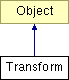
\includegraphics[height=2cm]{classm3g_1_1Transform}
\end{center}
\end{figure}
\subsection*{Public メソッド}
\begin{CompactItemize}
\item 
\hyperlink{classm3g_1_1Transform_9de68ec1c9b7809129814a3233ae4655}{Transform} ()
\item 
\hyperlink{classm3g_1_1Transform_6f8c18ec2bd6b5c0d7f3472752ec79d1}{Transform} (const \hyperlink{classm3g_1_1Transform}{Transform} \&t)
\item 
\hyperlink{classm3g_1_1Transform_8e627263611a76aad02c9e0b89287c68}{$\sim$Transform} ()
\item 
void \hyperlink{classm3g_1_1Transform_f78faf7dcc06f53604ad08965babb7b3}{get} (float $\ast$matrix) const 
\item 
\hyperlink{classm3g_1_1Matrix}{Matrix} \hyperlink{classm3g_1_1Transform_3ab68d9aa9eafd77e47631467de93f6f}{getMatrix} () const 
\item 
void \hyperlink{classm3g_1_1Transform_7fa1616cc61c19a5efcc863c950f7f30}{invert} ()
\item 
void \hyperlink{classm3g_1_1Transform_ad6083d90dbecc7e5bb39d5062723a0d}{postMultiply} (const \hyperlink{classm3g_1_1Transform}{Transform} \&transform)
\item 
void \hyperlink{classm3g_1_1Transform_4abf135257f132cdf9580f3a3e11ea6c}{postRotate} (float angle, float ax, float ay, float az)
\item 
void \hyperlink{classm3g_1_1Transform_7ce6ca00ac17bc4bb5f271c48da5e2dc}{postRotateQuat} (float qx, float qy, float qz, float qw)
\item 
void \hyperlink{classm3g_1_1Transform_4cbb4aa3878b658da54a144896f71446}{postScale} (float sx, float sy, float sz)
\item 
void \hyperlink{classm3g_1_1Transform_638498b811d6ccdf60b7f1f3de157ed6}{postTranslate} (float tx, float ty, float tz)
\item 
void \hyperlink{classm3g_1_1Transform_d1a2203142a848286c80d66c8c7fa37d}{set} (const float $\ast$matrix)
\item 
void \hyperlink{classm3g_1_1Transform_8926ff19517a76de8f938025e9d3163d}{set} (const \hyperlink{classm3g_1_1Transform}{Transform} \&transform)
\item 
void \hyperlink{classm3g_1_1Transform_18ea3e0bff5da78a203fa770a5cfee97}{set} (const \hyperlink{classm3g_1_1Matrix}{Matrix} \&matrix)
\item 
void \hyperlink{classm3g_1_1Transform_382e6ad7e6721b121e510959e1011be3}{setIdentity} ()
\item 
void \hyperlink{classm3g_1_1Transform_441599a6e846a344be78571668406619}{transform} (int vector\_\-num, float $\ast$vectors) const 
\item 
void \hyperlink{classm3g_1_1Transform_930167bb932a1c26c160fa1eece500d3}{transform} (const \hyperlink{classm3g_1_1VertexArray}{VertexArray} $\ast$in, float $\ast$out, bool w) const 
\item 
\hypertarget{classm3g_1_1Transform_46832c09c309a900fdab65b15bb5e8a7}{
\hyperlink{classm3g_1_1Vector}{Vector} \textbf{transform} (const \hyperlink{classm3g_1_1Vector}{Vector} \&vector) const }
\label{classm3g_1_1Transform_46832c09c309a900fdab65b15bb5e8a7}

\item 
\hypertarget{classm3g_1_1Transform_a8e4316680257437453501e30518a418}{
\hyperlink{classm3g_1_1Vector}{Vector} \textbf{transform3x3} (const \hyperlink{classm3g_1_1Vector}{Vector} \&vector) const }
\label{classm3g_1_1Transform_a8e4316680257437453501e30518a418}

\item 
void \hyperlink{classm3g_1_1Transform_f3a99ffb20127be48232d12260e934dc}{transpose} ()
\item 
virtual std::ostream \& \hyperlink{classm3g_1_1Transform_6fea17fa1532df3794f8cb39cb4f911f}{print} (std::ostream \&out) const 
\end{CompactItemize}


\subsection{説明}
座標変換を表す汎用の4x4行列. 

\subsection{コンストラクタとデストラクタ}
\hypertarget{classm3g_1_1Transform_9de68ec1c9b7809129814a3233ae4655}{
\index{m3g::Transform@{m3g::Transform}!Transform@{Transform}}
\index{Transform@{Transform}!m3g::Transform@{m3g::Transform}}
\subsubsection[{Transform}]{\setlength{\rightskip}{0pt plus 5cm}{\bf Transform} ()}}
\label{classm3g_1_1Transform_9de68ec1c9b7809129814a3233ae4655}


デフォルトの値のTransformオブジェクトの生成. \hypertarget{classm3g_1_1Transform_6f8c18ec2bd6b5c0d7f3472752ec79d1}{
\index{m3g::Transform@{m3g::Transform}!Transform@{Transform}}
\index{Transform@{Transform}!m3g::Transform@{m3g::Transform}}
\subsubsection[{Transform}]{\setlength{\rightskip}{0pt plus 5cm}{\bf Transform} (const {\bf Transform} \& {\em t})}}
\label{classm3g_1_1Transform_6f8c18ec2bd6b5c0d7f3472752ec79d1}


指定されたTransformをコピーしてTransformオブジェクトを生成. \hypertarget{classm3g_1_1Transform_8e627263611a76aad02c9e0b89287c68}{
\index{m3g::Transform@{m3g::Transform}!$\sim$Transform@{$\sim$Transform}}
\index{$\sim$Transform@{$\sim$Transform}!m3g::Transform@{m3g::Transform}}
\subsubsection[{$\sim$Transform}]{\setlength{\rightskip}{0pt plus 5cm}$\sim${\bf Transform} ()}}
\label{classm3g_1_1Transform_8e627263611a76aad02c9e0b89287c68}


このオブジェクトを削除するデストラクタ. 

\subsection{関数}
\hypertarget{classm3g_1_1Transform_f78faf7dcc06f53604ad08965babb7b3}{
\index{m3g::Transform@{m3g::Transform}!get@{get}}
\index{get@{get}!m3g::Transform@{m3g::Transform}}
\subsubsection[{get}]{\setlength{\rightskip}{0pt plus 5cm}void get (float $\ast$ {\em matrix}) const}}
\label{classm3g_1_1Transform_f78faf7dcc06f53604ad08965babb7b3}


この変換を16個のfloatの配列として取り出す. \hypertarget{classm3g_1_1Transform_3ab68d9aa9eafd77e47631467de93f6f}{
\index{m3g::Transform@{m3g::Transform}!getMatrix@{getMatrix}}
\index{getMatrix@{getMatrix}!m3g::Transform@{m3g::Transform}}
\subsubsection[{getMatrix}]{\setlength{\rightskip}{0pt plus 5cm}{\bf Matrix} getMatrix () const}}
\label{classm3g_1_1Transform_3ab68d9aa9eafd77e47631467de93f6f}


M3G非標準. \hypertarget{classm3g_1_1Transform_7fa1616cc61c19a5efcc863c950f7f30}{
\index{m3g::Transform@{m3g::Transform}!invert@{invert}}
\index{invert@{invert}!m3g::Transform@{m3g::Transform}}
\subsubsection[{invert}]{\setlength{\rightskip}{0pt plus 5cm}void invert ()}}
\label{classm3g_1_1Transform_7fa1616cc61c19a5efcc863c950f7f30}


(可能なら)この行列の逆行列を計算し置き換える. \hypertarget{classm3g_1_1Transform_ad6083d90dbecc7e5bb39d5062723a0d}{
\index{m3g::Transform@{m3g::Transform}!postMultiply@{postMultiply}}
\index{postMultiply@{postMultiply}!m3g::Transform@{m3g::Transform}}
\subsubsection[{postMultiply}]{\setlength{\rightskip}{0pt plus 5cm}void postMultiply (const {\bf Transform} \& {\em transform})}}
\label{classm3g_1_1Transform_ad6083d90dbecc7e5bb39d5062723a0d}


指定された変換行列を右から乗算する. \hypertarget{classm3g_1_1Transform_4abf135257f132cdf9580f3a3e11ea6c}{
\index{m3g::Transform@{m3g::Transform}!postRotate@{postRotate}}
\index{postRotate@{postRotate}!m3g::Transform@{m3g::Transform}}
\subsubsection[{postRotate}]{\setlength{\rightskip}{0pt plus 5cm}void postRotate (float {\em angle}, \/  float {\em ax}, \/  float {\em ay}, \/  float {\em az})}}
\label{classm3g_1_1Transform_4abf135257f132cdf9580f3a3e11ea6c}


指定された回転軸と角度で回転する回転行列を右から乗算する。角度の単位はdegree. \hypertarget{classm3g_1_1Transform_7ce6ca00ac17bc4bb5f271c48da5e2dc}{
\index{m3g::Transform@{m3g::Transform}!postRotateQuat@{postRotateQuat}}
\index{postRotateQuat@{postRotateQuat}!m3g::Transform@{m3g::Transform}}
\subsubsection[{postRotateQuat}]{\setlength{\rightskip}{0pt plus 5cm}void postRotateQuat (float {\em qx}, \/  float {\em qy}, \/  float {\em qz}, \/  float {\em qw})}}
\label{classm3g_1_1Transform_7ce6ca00ac17bc4bb5f271c48da5e2dc}


クォータニオン形式で指定された回転を行う回転行列を右から乗算する. \hypertarget{classm3g_1_1Transform_4cbb4aa3878b658da54a144896f71446}{
\index{m3g::Transform@{m3g::Transform}!postScale@{postScale}}
\index{postScale@{postScale}!m3g::Transform@{m3g::Transform}}
\subsubsection[{postScale}]{\setlength{\rightskip}{0pt plus 5cm}void postScale (float {\em sx}, \/  float {\em sy}, \/  float {\em sz})}}
\label{classm3g_1_1Transform_4cbb4aa3878b658da54a144896f71446}


指定されたスケーリング行列を右から乗算する. \hypertarget{classm3g_1_1Transform_638498b811d6ccdf60b7f1f3de157ed6}{
\index{m3g::Transform@{m3g::Transform}!postTranslate@{postTranslate}}
\index{postTranslate@{postTranslate}!m3g::Transform@{m3g::Transform}}
\subsubsection[{postTranslate}]{\setlength{\rightskip}{0pt plus 5cm}void postTranslate (float {\em tx}, \/  float {\em ty}, \/  float {\em tz})}}
\label{classm3g_1_1Transform_638498b811d6ccdf60b7f1f3de157ed6}


指定された移動行列を右から乗算する. \hypertarget{classm3g_1_1Transform_6fea17fa1532df3794f8cb39cb4f911f}{
\index{m3g::Transform@{m3g::Transform}!print@{print}}
\index{print@{print}!m3g::Transform@{m3g::Transform}}
\subsubsection[{print}]{\setlength{\rightskip}{0pt plus 5cm}std::ostream \& print (std::ostream \& {\em out}) const\hspace{0.3cm}{\tt  \mbox{[}virtual\mbox{]}}}}
\label{classm3g_1_1Transform_6fea17fa1532df3794f8cb39cb4f911f}


このTransformクラスの情報を表示する。デバッグ用. 

\hyperlink{classm3g_1_1Object_6fea17fa1532df3794f8cb39cb4f911f}{Object}を再定義しています。\hypertarget{classm3g_1_1Transform_18ea3e0bff5da78a203fa770a5cfee97}{
\index{m3g::Transform@{m3g::Transform}!set@{set}}
\index{set@{set}!m3g::Transform@{m3g::Transform}}
\subsubsection[{set}]{\setlength{\rightskip}{0pt plus 5cm}void set (const {\bf Matrix} \& {\em matrix})}}
\label{classm3g_1_1Transform_18ea3e0bff5da78a203fa770a5cfee97}


M3G非標準. \hypertarget{classm3g_1_1Transform_8926ff19517a76de8f938025e9d3163d}{
\index{m3g::Transform@{m3g::Transform}!set@{set}}
\index{set@{set}!m3g::Transform@{m3g::Transform}}
\subsubsection[{set}]{\setlength{\rightskip}{0pt plus 5cm}void set (const {\bf Transform} \& {\em transform})}}
\label{classm3g_1_1Transform_8926ff19517a76de8f938025e9d3163d}


指定されたTransformをコピーして変換を設定する. \hypertarget{classm3g_1_1Transform_d1a2203142a848286c80d66c8c7fa37d}{
\index{m3g::Transform@{m3g::Transform}!set@{set}}
\index{set@{set}!m3g::Transform@{m3g::Transform}}
\subsubsection[{set}]{\setlength{\rightskip}{0pt plus 5cm}void set (const float $\ast$ {\em matrix})}}
\label{classm3g_1_1Transform_d1a2203142a848286c80d66c8c7fa37d}


指定された16個のfloatの配列をコピーして変換を設定する. \hypertarget{classm3g_1_1Transform_382e6ad7e6721b121e510959e1011be3}{
\index{m3g::Transform@{m3g::Transform}!setIdentity@{setIdentity}}
\index{setIdentity@{setIdentity}!m3g::Transform@{m3g::Transform}}
\subsubsection[{setIdentity}]{\setlength{\rightskip}{0pt plus 5cm}void setIdentity ()}}
\label{classm3g_1_1Transform_382e6ad7e6721b121e510959e1011be3}


この変換を4x4の単位行列に設定する. \hypertarget{classm3g_1_1Transform_930167bb932a1c26c160fa1eece500d3}{
\index{m3g::Transform@{m3g::Transform}!transform@{transform}}
\index{transform@{transform}!m3g::Transform@{m3g::Transform}}
\subsubsection[{transform}]{\setlength{\rightskip}{0pt plus 5cm}void transform (const {\bf VertexArray} $\ast$ {\em in}, \/  float $\ast$ {\em out}, \/  bool {\em w}) const}}
\label{classm3g_1_1Transform_930167bb932a1c26c160fa1eece500d3}


指定されたVertexArrayの要素にこの変換行列を乗算する。 結果はfloatの配列として収納する. \hypertarget{classm3g_1_1Transform_441599a6e846a344be78571668406619}{
\index{m3g::Transform@{m3g::Transform}!transform@{transform}}
\index{transform@{transform}!m3g::Transform@{m3g::Transform}}
\subsubsection[{transform}]{\setlength{\rightskip}{0pt plus 5cm}void transform (int {\em vector\_\-num}, \/  float $\ast$ {\em vectors}) const}}
\label{classm3g_1_1Transform_441599a6e846a344be78571668406619}


指定された4要素のfloatのベクトルにこの変換行列を乗算する. \hypertarget{classm3g_1_1Transform_f3a99ffb20127be48232d12260e934dc}{
\index{m3g::Transform@{m3g::Transform}!transpose@{transpose}}
\index{transpose@{transpose}!m3g::Transform@{m3g::Transform}}
\subsubsection[{transpose}]{\setlength{\rightskip}{0pt plus 5cm}void transpose ()}}
\label{classm3g_1_1Transform_f3a99ffb20127be48232d12260e934dc}


転置を取りこの行列と入れ替える. 

このクラスの説明は次のファイルから生成されました:\begin{CompactItemize}
\item 
/work/workspace.desktop-m3g/src/Transform.hpp\item 
/work/workspace.desktop-m3g/src/Transform.cpp\end{CompactItemize}

\hypertarget{classm3g_1_1Transformable}{
\section{Transformable Class Reference}
\label{classm3g_1_1Transformable}\index{m3g::Transformable@{m3g::Transformable}}
}
{\tt \#include $<$Transformable.hpp$>$}

Inheritance diagram for Transformable::\begin{figure}[H]
\begin{center}
\leavevmode
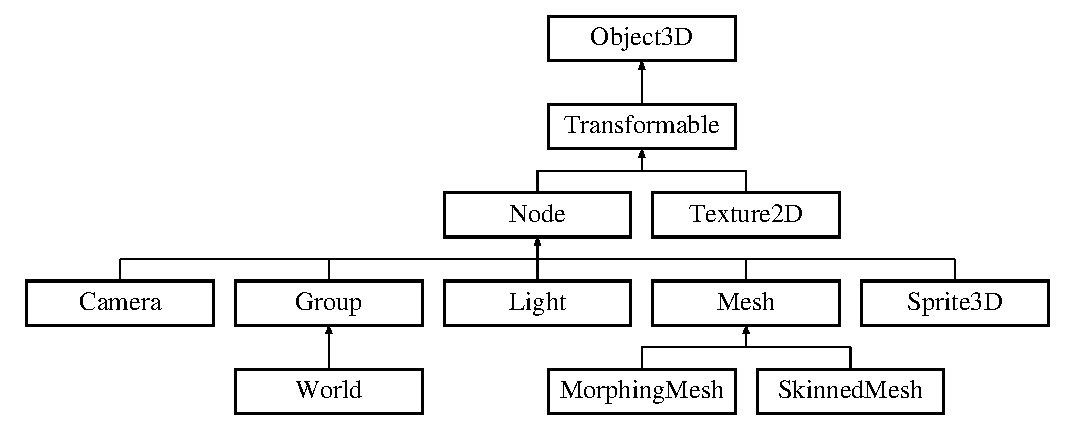
\includegraphics[height=5cm]{classm3g_1_1Transformable}
\end{center}
\end{figure}
\subsection*{Classes}
\begin{CompactItemize}
\item 
struct \textbf{Scale}
\item 
struct \textbf{Translation}
\end{CompactItemize}
\subsection*{Public Member Functions}
\begin{CompactItemize}
\item 
\hyperlink{classm3g_1_1Transformable_ca6563203e3e883391c9d0927028aa04}{Transformable} ()
\item 
virtual \hyperlink{classm3g_1_1Transformable_89d9c7912ed11a30a312fd8f72b9ab22}{$\sim$Transformable} ()
\item 
virtual void \hyperlink{classm3g_1_1Transformable_415c0b110f95410ded9b85e5d99a496b}{addAnimationTrack} (\hyperlink{classm3g_1_1AnimationTrack}{AnimationTrack} $\ast$animation\_\-track)
\item 
virtual int \hyperlink{classm3g_1_1Transformable_8aad1ceab4c2a03609c8a42324ce484d}{animate} (int world\_\-time)
\item 
void \hyperlink{classm3g_1_1Transformable_263ef66efed11b7f9678e2e4bbec4c55}{getCompositeTransform} (\hyperlink{classm3g_1_1Transform}{Transform} $\ast$transform) const 
\item 
void \hyperlink{classm3g_1_1Transformable_06125ab0d85ef8c5c7ace9ced04993f3}{getOrientation} (float $\ast$angle\_\-aixs) const 
\item 
void \hyperlink{classm3g_1_1Transformable_b8a2dd11d0ba90e138625eb86a6a6083}{getScale} (float $\ast$xyz) const 
\item 
void \hyperlink{classm3g_1_1Transformable_73f387f99c527b382c8aaa54b8af6ed6}{getTransform} (\hyperlink{classm3g_1_1Transform}{Transform} $\ast$transform) const 
\item 
void \hyperlink{classm3g_1_1Transformable_d8aec42959fecc3d76f9539d3afa3c8d}{getTranslation} (float $\ast$xyz) const 
\item 
void \hyperlink{classm3g_1_1Transformable_4abf135257f132cdf9580f3a3e11ea6c}{postRotate} (float angle, float ax, float ay, float az)
\item 
void \hyperlink{classm3g_1_1Transformable_718b606184672eec83263ad44d5c7431}{preRotate} (float angle, float ax, float ay, float az)
\item 
void \hyperlink{classm3g_1_1Transformable_d94deaf828db5e2dfd5e40db42b64cd9}{scale} (float sx, float sy, float sz)
\item 
void \hyperlink{classm3g_1_1Transformable_980a9a2b5f6102763042e616d3aa4606}{setOrientation} (float angle, float ax, float ay, float az)
\item 
void \hyperlink{classm3g_1_1Transformable_937d04042c25021532ea2532fe5e3a32}{setScale} (float sx, float sy, float sz)
\item 
void \hyperlink{classm3g_1_1Transformable_05052269aaf19775f3ff1a10d042777e}{setTransform} (const \hyperlink{classm3g_1_1Transform}{Transform} \&transform)
\item 
void \hyperlink{classm3g_1_1Transformable_afd728a7db85b8e12bdafc2b3c08a515}{setTranslation} (float tx, float ty, float tz)
\item 
void \hyperlink{classm3g_1_1Transformable_66d493b8307a85e615c4eb89116f2e09}{translate} (float tx, float ty, float tz)
\item 
virtual std::ostream \& \hyperlink{classm3g_1_1Transformable_6fea17fa1532df3794f8cb39cb4f911f}{print} (std::ostream \&out) const 
\end{CompactItemize}
\subsection*{Protected Member Functions}
\begin{CompactItemize}
\item 
virtual void \hyperlink{classm3g_1_1Transformable_1efcb1973989d9963d5bd6d03065d389}{render} (int pass, int index=0) const 
\end{CompactItemize}


\subsection{Detailed Description}
An abstract base class for \hyperlink{classm3g_1_1Node}{Node} and \hyperlink{classm3g_1_1Texture2D}{Texture2D}, defining common methods for manipulating node and texture. 

\subsection{Constructor \& Destructor Documentation}
\hypertarget{classm3g_1_1Transformable_ca6563203e3e883391c9d0927028aa04}{
\index{m3g::Transformable@{m3g::Transformable}!Transformable@{Transformable}}
\index{Transformable@{Transformable}!m3g::Transformable@{m3g::Transformable}}
\subsubsection[{Transformable}]{\setlength{\rightskip}{0pt plus 5cm}{\bf Transformable} ()}}
\label{classm3g_1_1Transformable_ca6563203e3e883391c9d0927028aa04}


Construct a new Tranformable object. \hypertarget{classm3g_1_1Transformable_89d9c7912ed11a30a312fd8f72b9ab22}{
\index{m3g::Transformable@{m3g::Transformable}!$\sim$Transformable@{$\sim$Transformable}}
\index{$\sim$Transformable@{$\sim$Transformable}!m3g::Transformable@{m3g::Transformable}}
\subsubsection[{$\sim$Transformable}]{\setlength{\rightskip}{0pt plus 5cm}$\sim${\bf Transformable} ()\hspace{0.3cm}{\tt  \mbox{[}virtual\mbox{]}}}}
\label{classm3g_1_1Transformable_89d9c7912ed11a30a312fd8f72b9ab22}


Destruct this object. 

\subsection{Member Function Documentation}
\hypertarget{classm3g_1_1Transformable_415c0b110f95410ded9b85e5d99a496b}{
\index{m3g::Transformable@{m3g::Transformable}!addAnimationTrack@{addAnimationTrack}}
\index{addAnimationTrack@{addAnimationTrack}!m3g::Transformable@{m3g::Transformable}}
\subsubsection[{addAnimationTrack}]{\setlength{\rightskip}{0pt plus 5cm}void addAnimationTrack ({\bf AnimationTrack} $\ast$ {\em animation\_\-track})\hspace{0.3cm}{\tt  \mbox{[}virtual\mbox{]}}}}
\label{classm3g_1_1Transformable_415c0b110f95410ded9b85e5d99a496b}


Adds the given \hyperlink{classm3g_1_1AnimationTrack}{AnimationTrack} to this \hyperlink{classm3g_1_1Object3D}{Object3D}, potentially changing the order and indices of the previously added tracks. 

Reimplemented from \hyperlink{classm3g_1_1Object3D_415c0b110f95410ded9b85e5d99a496b}{Object3D}.

Reimplemented in \hyperlink{classm3g_1_1Camera_415c0b110f95410ded9b85e5d99a496b}{Camera}, \hyperlink{classm3g_1_1Light_415c0b110f95410ded9b85e5d99a496b}{Light}, \hyperlink{classm3g_1_1MorphingMesh_415c0b110f95410ded9b85e5d99a496b}{MorphingMesh}, \hyperlink{classm3g_1_1Node_415c0b110f95410ded9b85e5d99a496b}{Node}, \hyperlink{classm3g_1_1Sprite3D_415c0b110f95410ded9b85e5d99a496b}{Sprite3D}, and \hyperlink{classm3g_1_1Texture2D_415c0b110f95410ded9b85e5d99a496b}{Texture2D}.\hypertarget{classm3g_1_1Transformable_8aad1ceab4c2a03609c8a42324ce484d}{
\index{m3g::Transformable@{m3g::Transformable}!animate@{animate}}
\index{animate@{animate}!m3g::Transformable@{m3g::Transformable}}
\subsubsection[{animate}]{\setlength{\rightskip}{0pt plus 5cm}int animate (int {\em world\_\-time})\hspace{0.3cm}{\tt  \mbox{[}virtual\mbox{]}}}}
\label{classm3g_1_1Transformable_8aad1ceab4c2a03609c8a42324ce484d}


Updates all animated properties in this \hyperlink{classm3g_1_1Object3D}{Object3D} and all Object3Ds that are reachable from this \hyperlink{classm3g_1_1Object3D}{Object3D}. 

Reimplemented from \hyperlink{classm3g_1_1Object3D_8aad1ceab4c2a03609c8a42324ce484d}{Object3D}.

Reimplemented in \hyperlink{classm3g_1_1Camera_8aad1ceab4c2a03609c8a42324ce484d}{Camera}, \hyperlink{classm3g_1_1Light_8aad1ceab4c2a03609c8a42324ce484d}{Light}, \hyperlink{classm3g_1_1Mesh_82cfeb67ca66b93e2ca7bda9a4f0e2aa}{Mesh}, \hyperlink{classm3g_1_1MorphingMesh_8aad1ceab4c2a03609c8a42324ce484d}{MorphingMesh}, \hyperlink{classm3g_1_1Node_8aad1ceab4c2a03609c8a42324ce484d}{Node}, \hyperlink{classm3g_1_1Sprite3D_8aad1ceab4c2a03609c8a42324ce484d}{Sprite3D}, \hyperlink{classm3g_1_1Texture2D_82cfeb67ca66b93e2ca7bda9a4f0e2aa}{Texture2D}, and \hyperlink{classm3g_1_1World_8aad1ceab4c2a03609c8a42324ce484d}{World}.\hypertarget{classm3g_1_1Transformable_263ef66efed11b7f9678e2e4bbec4c55}{
\index{m3g::Transformable@{m3g::Transformable}!getCompositeTransform@{getCompositeTransform}}
\index{getCompositeTransform@{getCompositeTransform}!m3g::Transformable@{m3g::Transformable}}
\subsubsection[{getCompositeTransform}]{\setlength{\rightskip}{0pt plus 5cm}void getCompositeTransform ({\bf Transform} $\ast$ {\em transform}) const}}
\label{classm3g_1_1Transformable_263ef66efed11b7f9678e2e4bbec4c55}


Retrieves the composite transformation matrix of this Transformabls. \hypertarget{classm3g_1_1Transformable_06125ab0d85ef8c5c7ace9ced04993f3}{
\index{m3g::Transformable@{m3g::Transformable}!getOrientation@{getOrientation}}
\index{getOrientation@{getOrientation}!m3g::Transformable@{m3g::Transformable}}
\subsubsection[{getOrientation}]{\setlength{\rightskip}{0pt plus 5cm}void getOrientation (float $\ast$ {\em angle\_\-aixs}) const}}
\label{classm3g_1_1Transformable_06125ab0d85ef8c5c7ace9ced04993f3}


Retriees the orientation component of htis \hyperlink{classm3g_1_1Transformable}{Transformable}. \hypertarget{classm3g_1_1Transformable_b8a2dd11d0ba90e138625eb86a6a6083}{
\index{m3g::Transformable@{m3g::Transformable}!getScale@{getScale}}
\index{getScale@{getScale}!m3g::Transformable@{m3g::Transformable}}
\subsubsection[{getScale}]{\setlength{\rightskip}{0pt plus 5cm}void getScale (float $\ast$ {\em xyz}) const}}
\label{classm3g_1_1Transformable_b8a2dd11d0ba90e138625eb86a6a6083}


Retrieves the matrix component of this \hyperlink{classm3g_1_1Transformable}{Transformable}. \hypertarget{classm3g_1_1Transformable_73f387f99c527b382c8aaa54b8af6ed6}{
\index{m3g::Transformable@{m3g::Transformable}!getTransform@{getTransform}}
\index{getTransform@{getTransform}!m3g::Transformable@{m3g::Transformable}}
\subsubsection[{getTransform}]{\setlength{\rightskip}{0pt plus 5cm}void getTransform ({\bf Transform} $\ast$ {\em transform}) const}}
\label{classm3g_1_1Transformable_73f387f99c527b382c8aaa54b8af6ed6}


Retrieves the matrix component of this Transofrmable. \hypertarget{classm3g_1_1Transformable_d8aec42959fecc3d76f9539d3afa3c8d}{
\index{m3g::Transformable@{m3g::Transformable}!getTranslation@{getTranslation}}
\index{getTranslation@{getTranslation}!m3g::Transformable@{m3g::Transformable}}
\subsubsection[{getTranslation}]{\setlength{\rightskip}{0pt plus 5cm}void getTranslation (float $\ast$ {\em xyz}) const}}
\label{classm3g_1_1Transformable_d8aec42959fecc3d76f9539d3afa3c8d}


Retrieves the translation component of this \hyperlink{classm3g_1_1Transformable}{Transformable}. \hypertarget{classm3g_1_1Transformable_4abf135257f132cdf9580f3a3e11ea6c}{
\index{m3g::Transformable@{m3g::Transformable}!postRotate@{postRotate}}
\index{postRotate@{postRotate}!m3g::Transformable@{m3g::Transformable}}
\subsubsection[{postRotate}]{\setlength{\rightskip}{0pt plus 5cm}void postRotate (float {\em angle}, \/  float {\em ax}, \/  float {\em ay}, \/  float {\em az})}}
\label{classm3g_1_1Transformable_4abf135257f132cdf9580f3a3e11ea6c}


Multiplies the current orientation component from the right by the given orientation. \hypertarget{classm3g_1_1Transformable_718b606184672eec83263ad44d5c7431}{
\index{m3g::Transformable@{m3g::Transformable}!preRotate@{preRotate}}
\index{preRotate@{preRotate}!m3g::Transformable@{m3g::Transformable}}
\subsubsection[{preRotate}]{\setlength{\rightskip}{0pt plus 5cm}void preRotate (float {\em angle}, \/  float {\em ax}, \/  float {\em ay}, \/  float {\em az})}}
\label{classm3g_1_1Transformable_718b606184672eec83263ad44d5c7431}


Multiplies the current orientation component from the left by the given orientation. \hypertarget{classm3g_1_1Transformable_6fea17fa1532df3794f8cb39cb4f911f}{
\index{m3g::Transformable@{m3g::Transformable}!print@{print}}
\index{print@{print}!m3g::Transformable@{m3g::Transformable}}
\subsubsection[{print}]{\setlength{\rightskip}{0pt plus 5cm}std::ostream \& print (std::ostream \& {\em out}) const\hspace{0.3cm}{\tt  \mbox{[}virtual\mbox{]}}}}
\label{classm3g_1_1Transformable_6fea17fa1532df3794f8cb39cb4f911f}


Print out information this object, for debug only. 

Reimplemented from \hyperlink{classm3g_1_1Object3D_6fea17fa1532df3794f8cb39cb4f911f}{Object3D}.

Reimplemented in \hyperlink{classm3g_1_1Camera_6fea17fa1532df3794f8cb39cb4f911f}{Camera}, \hyperlink{classm3g_1_1Light_6fea17fa1532df3794f8cb39cb4f911f}{Light}, \hyperlink{classm3g_1_1Mesh_6fea17fa1532df3794f8cb39cb4f911f}{Mesh}, \hyperlink{classm3g_1_1MorphingMesh_6fea17fa1532df3794f8cb39cb4f911f}{MorphingMesh}, \hyperlink{classm3g_1_1Node_6fea17fa1532df3794f8cb39cb4f911f}{Node}, \hyperlink{classm3g_1_1SkinnedMesh_6fea17fa1532df3794f8cb39cb4f911f}{SkinnedMesh}, \hyperlink{classm3g_1_1Sprite3D_6fea17fa1532df3794f8cb39cb4f911f}{Sprite3D}, \hyperlink{classm3g_1_1Texture2D_6fea17fa1532df3794f8cb39cb4f911f}{Texture2D}, and \hyperlink{classm3g_1_1World_6fea17fa1532df3794f8cb39cb4f911f}{World}.\hypertarget{classm3g_1_1Transformable_1efcb1973989d9963d5bd6d03065d389}{
\index{m3g::Transformable@{m3g::Transformable}!render@{render}}
\index{render@{render}!m3g::Transformable@{m3g::Transformable}}
\subsubsection[{render}]{\setlength{\rightskip}{0pt plus 5cm}void render (int {\em pass}, \/  int {\em index} = {\tt 0}) const\hspace{0.3cm}{\tt  \mbox{[}protected, virtual\mbox{]}}}}
\label{classm3g_1_1Transformable_1efcb1973989d9963d5bd6d03065d389}


Render this object, for inner use. 

Reimplemented from \hyperlink{classm3g_1_1Object3D_1efcb1973989d9963d5bd6d03065d389}{Object3D}.

Reimplemented in \hyperlink{classm3g_1_1Camera_1efcb1973989d9963d5bd6d03065d389}{Camera}, \hyperlink{classm3g_1_1Mesh_1efcb1973989d9963d5bd6d03065d389}{Mesh}, \hyperlink{classm3g_1_1MorphingMesh_1efcb1973989d9963d5bd6d03065d389}{MorphingMesh}, \hyperlink{classm3g_1_1Node_1efcb1973989d9963d5bd6d03065d389}{Node}, \hyperlink{classm3g_1_1SkinnedMesh_1efcb1973989d9963d5bd6d03065d389}{SkinnedMesh}, \hyperlink{classm3g_1_1Sprite3D_1efcb1973989d9963d5bd6d03065d389}{Sprite3D}, and \hyperlink{classm3g_1_1World_1efcb1973989d9963d5bd6d03065d389}{World}.\hypertarget{classm3g_1_1Transformable_d94deaf828db5e2dfd5e40db42b64cd9}{
\index{m3g::Transformable@{m3g::Transformable}!scale@{scale}}
\index{scale@{scale}!m3g::Transformable@{m3g::Transformable}}
\subsubsection[{scale}]{\setlength{\rightskip}{0pt plus 5cm}void scale (float {\em sx}, \/  float {\em sy}, \/  float {\em sz})}}
\label{classm3g_1_1Transformable_d94deaf828db5e2dfd5e40db42b64cd9}


Multiplies the current scale component by the given scale factors. \hypertarget{classm3g_1_1Transformable_980a9a2b5f6102763042e616d3aa4606}{
\index{m3g::Transformable@{m3g::Transformable}!setOrientation@{setOrientation}}
\index{setOrientation@{setOrientation}!m3g::Transformable@{m3g::Transformable}}
\subsubsection[{setOrientation}]{\setlength{\rightskip}{0pt plus 5cm}void setOrientation (float {\em angle}, \/  float {\em ax}, \/  float {\em ay}, \/  float {\em az})}}
\label{classm3g_1_1Transformable_980a9a2b5f6102763042e616d3aa4606}


Sets the orientation component of this \hyperlink{classm3g_1_1Transformable}{Transformable}. \hypertarget{classm3g_1_1Transformable_937d04042c25021532ea2532fe5e3a32}{
\index{m3g::Transformable@{m3g::Transformable}!setScale@{setScale}}
\index{setScale@{setScale}!m3g::Transformable@{m3g::Transformable}}
\subsubsection[{setScale}]{\setlength{\rightskip}{0pt plus 5cm}void setScale (float {\em sx}, \/  float {\em sy}, \/  float {\em sz})}}
\label{classm3g_1_1Transformable_937d04042c25021532ea2532fe5e3a32}


Sets the scale component of this \hyperlink{classm3g_1_1Transformable}{Transformable}. \hypertarget{classm3g_1_1Transformable_05052269aaf19775f3ff1a10d042777e}{
\index{m3g::Transformable@{m3g::Transformable}!setTransform@{setTransform}}
\index{setTransform@{setTransform}!m3g::Transformable@{m3g::Transformable}}
\subsubsection[{setTransform}]{\setlength{\rightskip}{0pt plus 5cm}void setTransform (const {\bf Transform} \& {\em transform})}}
\label{classm3g_1_1Transformable_05052269aaf19775f3ff1a10d042777e}


Sets the matrix component of this \hyperlink{classm3g_1_1Transformable}{Transformable} by copying in the given \hyperlink{classm3g_1_1Transform}{Transform}. \hypertarget{classm3g_1_1Transformable_afd728a7db85b8e12bdafc2b3c08a515}{
\index{m3g::Transformable@{m3g::Transformable}!setTranslation@{setTranslation}}
\index{setTranslation@{setTranslation}!m3g::Transformable@{m3g::Transformable}}
\subsubsection[{setTranslation}]{\setlength{\rightskip}{0pt plus 5cm}void setTranslation (float {\em tx}, \/  float {\em ty}, \/  float {\em tz})}}
\label{classm3g_1_1Transformable_afd728a7db85b8e12bdafc2b3c08a515}


Sets the translation component of this \hyperlink{classm3g_1_1Transformable}{Transformable}. \hypertarget{classm3g_1_1Transformable_66d493b8307a85e615c4eb89116f2e09}{
\index{m3g::Transformable@{m3g::Transformable}!translate@{translate}}
\index{translate@{translate}!m3g::Transformable@{m3g::Transformable}}
\subsubsection[{translate}]{\setlength{\rightskip}{0pt plus 5cm}void translate (float {\em tx}, \/  float {\em ty}, \/  float {\em tz})}}
\label{classm3g_1_1Transformable_66d493b8307a85e615c4eb89116f2e09}


Adds the given offset to the current translation component. 

The documentation for this class was generated from the following files:\begin{CompactItemize}
\item 
/work/desktop-m3g/src/Transformable.hpp\item 
/work/desktop-m3g/src/Transformable.cpp\end{CompactItemize}

\hypertarget{classm3g_1_1TriangleStripArray}{
\section{TriangleStripArray Class Reference}
\label{classm3g_1_1TriangleStripArray}\index{m3g::TriangleStripArray@{m3g::TriangleStripArray}}
}
{\tt \#include $<$TriangleStripArray.hpp$>$}

Inheritance diagram for TriangleStripArray::\begin{figure}[H]
\begin{center}
\leavevmode
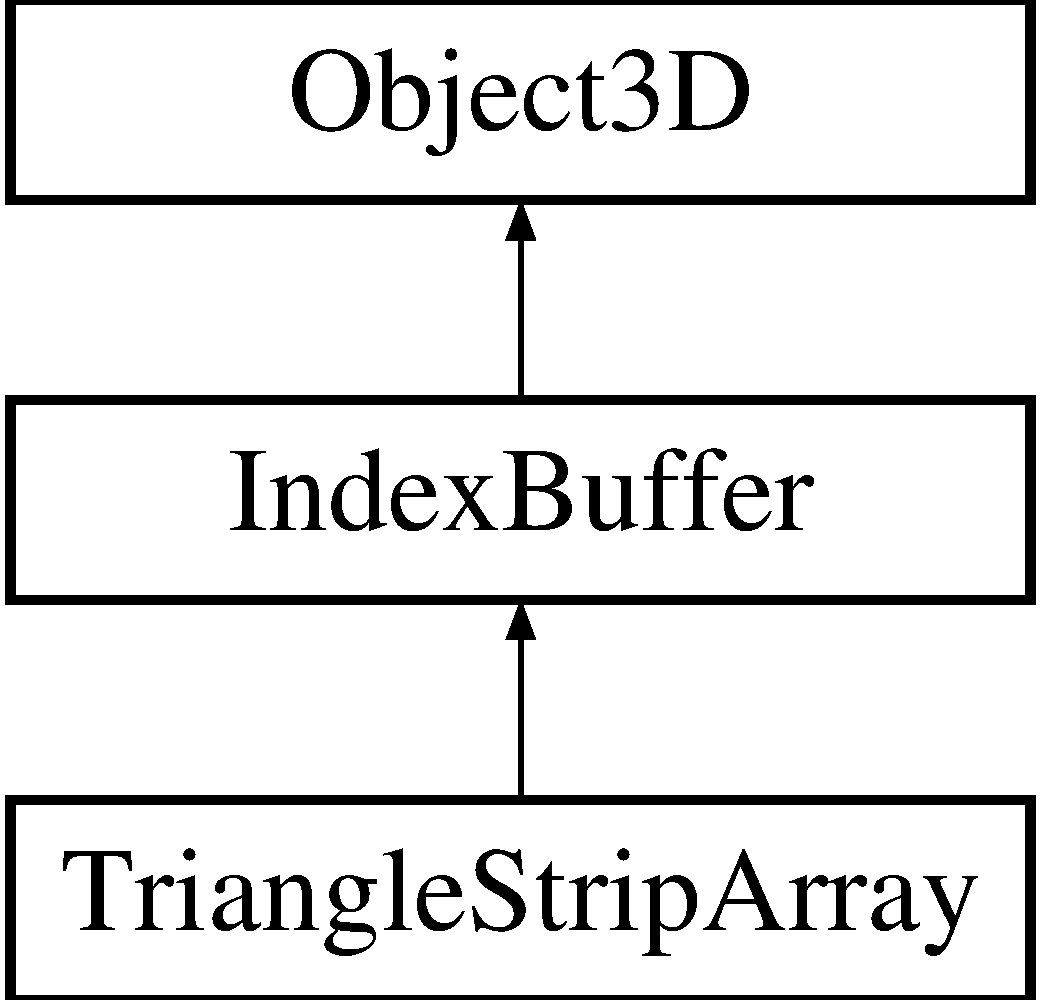
\includegraphics[height=3cm]{classm3g_1_1TriangleStripArray}
\end{center}
\end{figure}
\subsection*{Public Member Functions}
\begin{CompactItemize}
\item 
\hyperlink{classm3g_1_1TriangleStripArray_57d4e874819367084aeadb11593c4436}{TriangleStripArray} (int $\ast$indices, int num\_\-strips, int $\ast$strips)
\item 
\hyperlink{classm3g_1_1TriangleStripArray_d2ca9884a6ccf32da3cee977549b5ee0}{TriangleStripArray} (int first\_\-index, int num\_\-strips, int $\ast$strips)
\item 
virtual \hyperlink{classm3g_1_1TriangleStripArray_1cb3853bf79b7710d57044da818d2cde}{$\sim$TriangleStripArray} ()
\item 
virtual int \hyperlink{classm3g_1_1TriangleStripArray_fe9ae2993ebcdb93d5ff26d57c81b73e}{getIndexCount} () const 
\item 
virtual void \hyperlink{classm3g_1_1TriangleStripArray_650953afac45099025a524ab160b911f}{getIndices} (int $\ast$indices)
\item 
virtual std::ostream \& \hyperlink{classm3g_1_1TriangleStripArray_6fea17fa1532df3794f8cb39cb4f911f}{print} (std::ostream \&out) const 
\end{CompactItemize}
\subsection*{Protected Member Functions}
\begin{CompactItemize}
\item 
virtual void \hyperlink{classm3g_1_1TriangleStripArray_1efcb1973989d9963d5bd6d03065d389}{render} (int pass, int index=0) const 
\end{CompactItemize}
\subsection*{Friends}
\begin{CompactItemize}
\item 
\hypertarget{classm3g_1_1TriangleStripArray_1f61169bea98d63b51332345ccaea9d5}{
class \textbf{UnitTest::Test}}
\label{classm3g_1_1TriangleStripArray_1f61169bea98d63b51332345ccaea9d5}

\end{CompactItemize}


\subsection{Detailed Description}
\hyperlink{classm3g_1_1TriangleStripArray}{TriangleStripArray} defines an array of triangle strips. 

\subsection{Constructor \& Destructor Documentation}
\hypertarget{classm3g_1_1TriangleStripArray_57d4e874819367084aeadb11593c4436}{
\index{m3g::TriangleStripArray@{m3g::TriangleStripArray}!TriangleStripArray@{TriangleStripArray}}
\index{TriangleStripArray@{TriangleStripArray}!m3g::TriangleStripArray@{m3g::TriangleStripArray}}
\subsubsection[{TriangleStripArray}]{\setlength{\rightskip}{0pt plus 5cm}{\bf TriangleStripArray} (int $\ast$ {\em indices}, \/  int {\em num\_\-strips}, \/  int $\ast$ {\em strips})}}
\label{classm3g_1_1TriangleStripArray_57d4e874819367084aeadb11593c4436}


Constructs a triangle strip array with explicit indices. \hypertarget{classm3g_1_1TriangleStripArray_d2ca9884a6ccf32da3cee977549b5ee0}{
\index{m3g::TriangleStripArray@{m3g::TriangleStripArray}!TriangleStripArray@{TriangleStripArray}}
\index{TriangleStripArray@{TriangleStripArray}!m3g::TriangleStripArray@{m3g::TriangleStripArray}}
\subsubsection[{TriangleStripArray}]{\setlength{\rightskip}{0pt plus 5cm}{\bf TriangleStripArray} (int {\em first\_\-index}, \/  int {\em num\_\-strips}, \/  int $\ast$ {\em strips})}}
\label{classm3g_1_1TriangleStripArray_d2ca9884a6ccf32da3cee977549b5ee0}


Constructs a triangle strip array with implicit indices. \hypertarget{classm3g_1_1TriangleStripArray_1cb3853bf79b7710d57044da818d2cde}{
\index{m3g::TriangleStripArray@{m3g::TriangleStripArray}!$\sim$TriangleStripArray@{$\sim$TriangleStripArray}}
\index{$\sim$TriangleStripArray@{$\sim$TriangleStripArray}!m3g::TriangleStripArray@{m3g::TriangleStripArray}}
\subsubsection[{$\sim$TriangleStripArray}]{\setlength{\rightskip}{0pt plus 5cm}$\sim${\bf TriangleStripArray} ()\hspace{0.3cm}{\tt  \mbox{[}virtual\mbox{]}}}}
\label{classm3g_1_1TriangleStripArray_1cb3853bf79b7710d57044da818d2cde}


Destruct this object. 

\subsection{Member Function Documentation}
\hypertarget{classm3g_1_1TriangleStripArray_fe9ae2993ebcdb93d5ff26d57c81b73e}{
\index{m3g::TriangleStripArray@{m3g::TriangleStripArray}!getIndexCount@{getIndexCount}}
\index{getIndexCount@{getIndexCount}!m3g::TriangleStripArray@{m3g::TriangleStripArray}}
\subsubsection[{getIndexCount}]{\setlength{\rightskip}{0pt plus 5cm}int getIndexCount () const\hspace{0.3cm}{\tt  \mbox{[}virtual\mbox{]}}}}
\label{classm3g_1_1TriangleStripArray_fe9ae2993ebcdb93d5ff26d57c81b73e}


Returns the number of indices in this buffer. 

Implements \hyperlink{classm3g_1_1IndexBuffer_ac7d2c37f177b21195a81f00061ef94e}{IndexBuffer}.\hypertarget{classm3g_1_1TriangleStripArray_650953afac45099025a524ab160b911f}{
\index{m3g::TriangleStripArray@{m3g::TriangleStripArray}!getIndices@{getIndices}}
\index{getIndices@{getIndices}!m3g::TriangleStripArray@{m3g::TriangleStripArray}}
\subsubsection[{getIndices}]{\setlength{\rightskip}{0pt plus 5cm}void getIndices (int $\ast$ {\em indices})\hspace{0.3cm}{\tt  \mbox{[}virtual\mbox{]}}}}
\label{classm3g_1_1TriangleStripArray_650953afac45099025a524ab160b911f}


Retrieves vertex indices for the rendering primitives stored in this buffer. 

Implements \hyperlink{classm3g_1_1IndexBuffer_59fb1eca8810ea3b028735c5dce53fca}{IndexBuffer}.\hypertarget{classm3g_1_1TriangleStripArray_6fea17fa1532df3794f8cb39cb4f911f}{
\index{m3g::TriangleStripArray@{m3g::TriangleStripArray}!print@{print}}
\index{print@{print}!m3g::TriangleStripArray@{m3g::TriangleStripArray}}
\subsubsection[{print}]{\setlength{\rightskip}{0pt plus 5cm}std::ostream \& print (std::ostream \& {\em out}) const\hspace{0.3cm}{\tt  \mbox{[}virtual\mbox{]}}}}
\label{classm3g_1_1TriangleStripArray_6fea17fa1532df3794f8cb39cb4f911f}


Print out information of this object, for debug only. 

Reimplemented from \hyperlink{classm3g_1_1IndexBuffer_6fea17fa1532df3794f8cb39cb4f911f}{IndexBuffer}.\hypertarget{classm3g_1_1TriangleStripArray_1efcb1973989d9963d5bd6d03065d389}{
\index{m3g::TriangleStripArray@{m3g::TriangleStripArray}!render@{render}}
\index{render@{render}!m3g::TriangleStripArray@{m3g::TriangleStripArray}}
\subsubsection[{render}]{\setlength{\rightskip}{0pt plus 5cm}void render (int {\em pass}, \/  int {\em index} = {\tt 0}) const\hspace{0.3cm}{\tt  \mbox{[}protected, virtual\mbox{]}}}}
\label{classm3g_1_1TriangleStripArray_1efcb1973989d9963d5bd6d03065d389}


Render this object, for inner use.

Note: \hyperlink{classm3g_1_1TriangleStripArray}{TriangleStripArray} should be rendered only at second rendering pass(pass=2). In other cases, do nothing. 

Reimplemented from \hyperlink{classm3g_1_1IndexBuffer_1efcb1973989d9963d5bd6d03065d389}{IndexBuffer}.

The documentation for this class was generated from the following files:\begin{CompactItemize}
\item 
/work/desktop-m3g/src/TriangleStripArray.hpp\item 
/work/desktop-m3g/src/TriangleStripArray.cpp\end{CompactItemize}

\hypertarget{classm3g_1_1VertexArray}{
\section{クラス VertexArray}
\label{classm3g_1_1VertexArray}\index{m3g::VertexArray@{m3g::VertexArray}}
}
{\tt \#include $<$VertexArray.hpp$>$}

VertexArrayに対する継承グラフ:\begin{figure}[H]
\begin{center}
\leavevmode
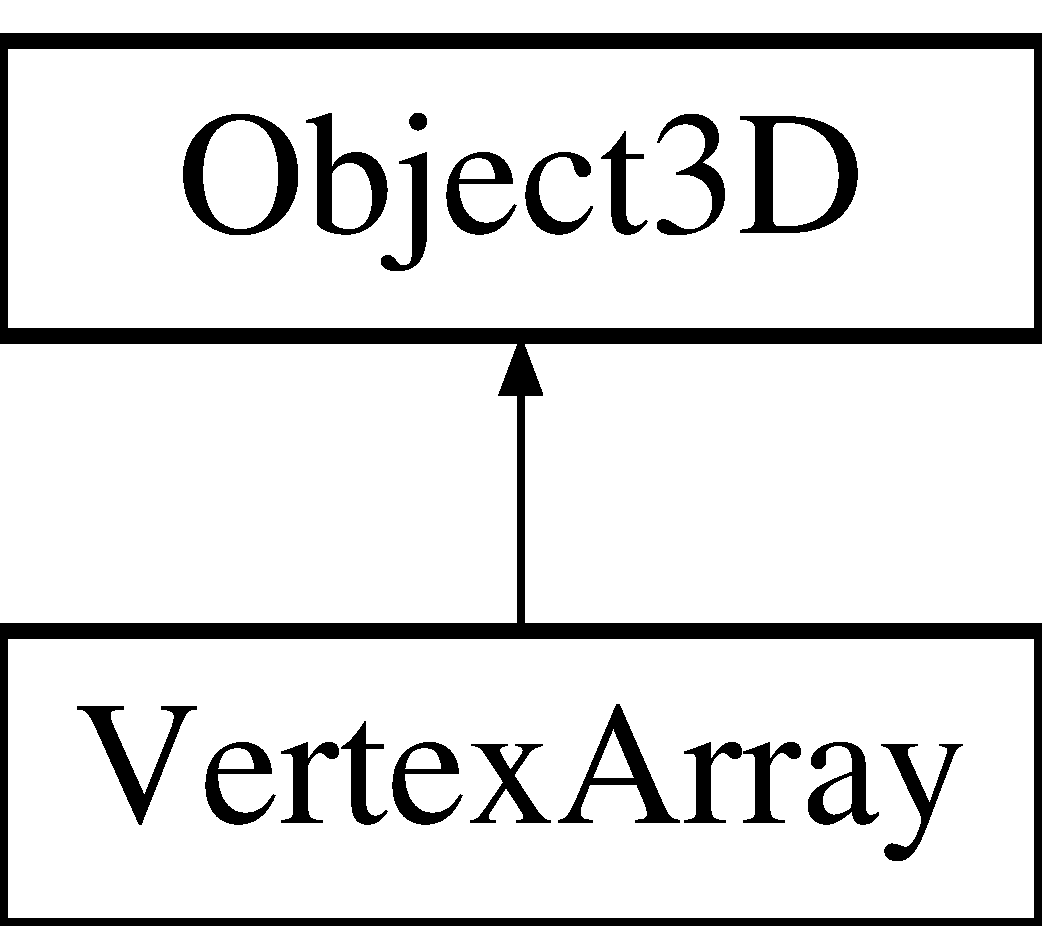
\includegraphics[height=2cm]{classm3g_1_1VertexArray}
\end{center}
\end{figure}
\subsection*{Public メソッド}
\begin{CompactItemize}
\item 
\hyperlink{classm3g_1_1VertexArray_5f38e30d23b5dc34b223e749e8afd0d0}{VertexArray} (int num\_\-vertices, int num\_\-components, int component\_\-size)
\item 
virtual \hyperlink{classm3g_1_1VertexArray_267fa63cb2f4216729437dc826415911}{$\sim$VertexArray} ()
\item 
void \hyperlink{classm3g_1_1VertexArray_9d1b801a7c196a07553a5ef4a5473573}{get} (int first\_\-vertex, int num\_\-vertices, char $\ast$values) const 
\item 
void \hyperlink{classm3g_1_1VertexArray_575822f60d7b5e74ed51e94851123038}{get} (int first\_\-vertex, int num\_\-vertices, short $\ast$values) const 
\item 
int \hyperlink{classm3g_1_1VertexArray_7016f51d2788e78fdd736efd040f5e5e}{getComponentCount} () const 
\item 
int \hyperlink{classm3g_1_1VertexArray_9b7b78fbff0603779ec6bdd2a323c939}{getComponentType} () const 
\item 
int \hyperlink{classm3g_1_1VertexArray_c1c9b7f5b0dcd9c0310d7e77e10081ba}{getVertexCount} () const 
\item 
void \hyperlink{classm3g_1_1VertexArray_501a9e6d9b5190b0a9dbfe58a6fd9d2e}{set} (int first\_\-vertex, int num\_\-vertices, char $\ast$values)
\item 
void \hyperlink{classm3g_1_1VertexArray_ac10afe01263d9ac5e7f972a7263de4a}{set} (int first\_\-vertex, int num\_\-vertices, short $\ast$values)
\item 
virtual std::ostream \& \hyperlink{classm3g_1_1VertexArray_6fea17fa1532df3794f8cb39cb4f911f}{print} (std::ostream \&out) const 
\item 
void \hyperlink{classm3g_1_1VertexArray_1adedf59e0c6a047242a3914ca52b929}{get} (int first\_\-vertex, int num\_\-vertices, float scale, float $\ast$bias, float $\ast$values) const 
\end{CompactItemize}
\subsection*{フレンド}
\begin{CompactItemize}
\item 
\hypertarget{classm3g_1_1VertexArray_9ef9a3db41cb54690169922706e1d3c5}{
class \textbf{VertexBuffer}}
\label{classm3g_1_1VertexArray_9ef9a3db41cb54690169922706e1d3c5}

\end{CompactItemize}


\subsection{説明}
頂点座標、頂点法線、頂点カラー、テクスチャー座標を表す整数ベクトルの配列. 

\subsection{コンストラクタとデストラクタ}
\hypertarget{classm3g_1_1VertexArray_5f38e30d23b5dc34b223e749e8afd0d0}{
\index{m3g::VertexArray@{m3g::VertexArray}!VertexArray@{VertexArray}}
\index{VertexArray@{VertexArray}!m3g::VertexArray@{m3g::VertexArray}}
\subsubsection[{VertexArray}]{\setlength{\rightskip}{0pt plus 5cm}{\bf VertexArray} (int {\em num\_\-vertices}, \/  int {\em num\_\-components}, \/  int {\em component\_\-size})}}
\label{classm3g_1_1VertexArray_5f38e30d23b5dc34b223e749e8afd0d0}


指定されたサイズで新しいVertxArrayを作成する. \hypertarget{classm3g_1_1VertexArray_267fa63cb2f4216729437dc826415911}{
\index{m3g::VertexArray@{m3g::VertexArray}!$\sim$VertexArray@{$\sim$VertexArray}}
\index{$\sim$VertexArray@{$\sim$VertexArray}!m3g::VertexArray@{m3g::VertexArray}}
\subsubsection[{$\sim$VertexArray}]{\setlength{\rightskip}{0pt plus 5cm}$\sim${\bf VertexArray} ()\hspace{0.3cm}{\tt  \mbox{[}virtual\mbox{]}}}}
\label{classm3g_1_1VertexArray_267fa63cb2f4216729437dc826415911}


このオブジェクトを削除するデストラクタ. 

\subsection{関数}
\hypertarget{classm3g_1_1VertexArray_1adedf59e0c6a047242a3914ca52b929}{
\index{m3g::VertexArray@{m3g::VertexArray}!get@{get}}
\index{get@{get}!m3g::VertexArray@{m3g::VertexArray}}
\subsubsection[{get}]{\setlength{\rightskip}{0pt plus 5cm}void get (int {\em first\_\-vertex}, \/  int {\em num\_\-vertices}, \/  float {\em scale}, \/  float $\ast$ {\em bias}, \/  float $\ast$ {\em values}) const}}
\label{classm3g_1_1VertexArray_1adedf59e0c6a047242a3914ca52b929}


値にscale,biasをかけてfloatで取り出すM3G非標準の関数. \hypertarget{classm3g_1_1VertexArray_575822f60d7b5e74ed51e94851123038}{
\index{m3g::VertexArray@{m3g::VertexArray}!get@{get}}
\index{get@{get}!m3g::VertexArray@{m3g::VertexArray}}
\subsubsection[{get}]{\setlength{\rightskip}{0pt plus 5cm}void get (int {\em first\_\-vertex}, \/  int {\em num\_\-vertices}, \/  short $\ast$ {\em values}) const}}
\label{classm3g_1_1VertexArray_575822f60d7b5e74ed51e94851123038}


16bit頂点属性値のレンジの取得. \hypertarget{classm3g_1_1VertexArray_9d1b801a7c196a07553a5ef4a5473573}{
\index{m3g::VertexArray@{m3g::VertexArray}!get@{get}}
\index{get@{get}!m3g::VertexArray@{m3g::VertexArray}}
\subsubsection[{get}]{\setlength{\rightskip}{0pt plus 5cm}void get (int {\em first\_\-vertex}, \/  int {\em num\_\-vertices}, \/  char $\ast$ {\em values}) const}}
\label{classm3g_1_1VertexArray_9d1b801a7c196a07553a5ef4a5473573}


8bit頂点属性値のレンジの取得. \hypertarget{classm3g_1_1VertexArray_7016f51d2788e78fdd736efd040f5e5e}{
\index{m3g::VertexArray@{m3g::VertexArray}!getComponentCount@{getComponentCount}}
\index{getComponentCount@{getComponentCount}!m3g::VertexArray@{m3g::VertexArray}}
\subsubsection[{getComponentCount}]{\setlength{\rightskip}{0pt plus 5cm}int getComponentCount () const}}
\label{classm3g_1_1VertexArray_7016f51d2788e78fdd736efd040f5e5e}


1頂点当たりの要素数の取得. \hypertarget{classm3g_1_1VertexArray_9b7b78fbff0603779ec6bdd2a323c939}{
\index{m3g::VertexArray@{m3g::VertexArray}!getComponentType@{getComponentType}}
\index{getComponentType@{getComponentType}!m3g::VertexArray@{m3g::VertexArray}}
\subsubsection[{getComponentType}]{\setlength{\rightskip}{0pt plus 5cm}int getComponentType () const}}
\label{classm3g_1_1VertexArray_9b7b78fbff0603779ec6bdd2a323c939}


頂点要素のデータタイプ(サイズ)の取得. \hypertarget{classm3g_1_1VertexArray_c1c9b7f5b0dcd9c0310d7e77e10081ba}{
\index{m3g::VertexArray@{m3g::VertexArray}!getVertexCount@{getVertexCount}}
\index{getVertexCount@{getVertexCount}!m3g::VertexArray@{m3g::VertexArray}}
\subsubsection[{getVertexCount}]{\setlength{\rightskip}{0pt plus 5cm}int getVertexCount () const}}
\label{classm3g_1_1VertexArray_c1c9b7f5b0dcd9c0310d7e77e10081ba}


この配列の超点数の取得. \hypertarget{classm3g_1_1VertexArray_6fea17fa1532df3794f8cb39cb4f911f}{
\index{m3g::VertexArray@{m3g::VertexArray}!print@{print}}
\index{print@{print}!m3g::VertexArray@{m3g::VertexArray}}
\subsubsection[{print}]{\setlength{\rightskip}{0pt plus 5cm}std::ostream \& print (std::ostream \& {\em out}) const\hspace{0.3cm}{\tt  \mbox{[}virtual\mbox{]}}}}
\label{classm3g_1_1VertexArray_6fea17fa1532df3794f8cb39cb4f911f}


このVertexArrayクラスの情報を表示する。デバッグ用. 

\hyperlink{classm3g_1_1Object3D_6fea17fa1532df3794f8cb39cb4f911f}{Object3D}を再定義しています。\hypertarget{classm3g_1_1VertexArray_ac10afe01263d9ac5e7f972a7263de4a}{
\index{m3g::VertexArray@{m3g::VertexArray}!set@{set}}
\index{set@{set}!m3g::VertexArray@{m3g::VertexArray}}
\subsubsection[{set}]{\setlength{\rightskip}{0pt plus 5cm}void set (int {\em first\_\-vertex}, \/  int {\em num\_\-vertices}, \/  short $\ast$ {\em values})}}
\label{classm3g_1_1VertexArray_ac10afe01263d9ac5e7f972a7263de4a}


16bit頂点属性値のコピー. \hypertarget{classm3g_1_1VertexArray_501a9e6d9b5190b0a9dbfe58a6fd9d2e}{
\index{m3g::VertexArray@{m3g::VertexArray}!set@{set}}
\index{set@{set}!m3g::VertexArray@{m3g::VertexArray}}
\subsubsection[{set}]{\setlength{\rightskip}{0pt plus 5cm}void set (int {\em first\_\-vertex}, \/  int {\em num\_\-vertices}, \/  char $\ast$ {\em values})}}
\label{classm3g_1_1VertexArray_501a9e6d9b5190b0a9dbfe58a6fd9d2e}


8bit頂点属性値のコピー. 

このクラスの説明は次のファイルから生成されました:\begin{CompactItemize}
\item 
/work/desktop-m3g/src/VertexArray.hpp\item 
/work/desktop-m3g/src/VertexArray.cpp\end{CompactItemize}

\hypertarget{classm3g_1_1VertexBuffer}{
\section{VertexBuffer Class Reference}
\label{classm3g_1_1VertexBuffer}\index{m3g::VertexBuffer@{m3g::VertexBuffer}}
}
{\tt \#include $<$VertexBuffer.hpp$>$}

Inheritance diagram for VertexBuffer::\begin{figure}[H]
\begin{center}
\leavevmode
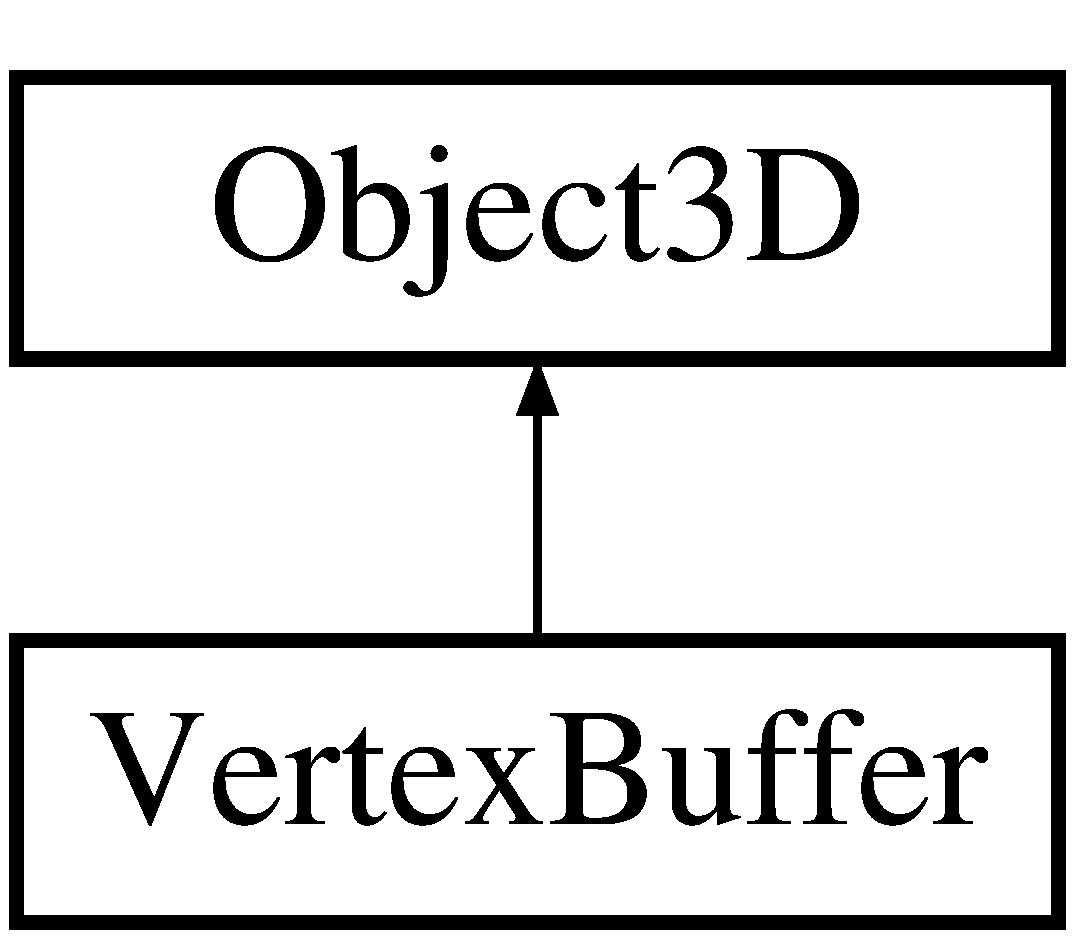
\includegraphics[height=2cm]{classm3g_1_1VertexBuffer}
\end{center}
\end{figure}
\subsection*{Public Member Functions}
\begin{CompactItemize}
\item 
\hyperlink{classm3g_1_1VertexBuffer_fd7b13840c99c57d27316c8f8434dc49}{VertexBuffer} ()
\item 
virtual \hyperlink{classm3g_1_1VertexBuffer_0e5e1dbdc4295ff9aa1e15e0ce3624af}{$\sim$VertexBuffer} ()
\item 
virtual void \hyperlink{classm3g_1_1VertexBuffer_415c0b110f95410ded9b85e5d99a496b}{addAnimationTrack} (\hyperlink{classm3g_1_1AnimationTrack}{AnimationTrack} $\ast$animation\_\-track)
\item 
virtual int \hyperlink{classm3g_1_1VertexBuffer_82cfeb67ca66b93e2ca7bda9a4f0e2aa}{animate} (int time)
\item 
\hyperlink{classm3g_1_1VertexArray}{VertexArray} $\ast$ \hyperlink{classm3g_1_1VertexBuffer_e3bdc8503242a6d278230352d03e5893}{getColors} () const 
\item 
int \hyperlink{classm3g_1_1VertexBuffer_4e33b93a98ce0632d51e7ae775ae5b1e}{getDefaultColor} () const 
\item 
\hyperlink{classm3g_1_1VertexArray}{VertexArray} $\ast$ \hyperlink{classm3g_1_1VertexBuffer_0f4341d1215ff8f4efeaa40a21327c0c}{getNormals} () const 
\item 
\hyperlink{classm3g_1_1VertexArray}{VertexArray} $\ast$ \hyperlink{classm3g_1_1VertexBuffer_5ca059361f9f834dd00b5d595bf3df0b}{getPositions} (float $\ast$scale\_\-bias) const 
\item 
\hyperlink{classm3g_1_1VertexArray}{VertexArray} $\ast$ \hyperlink{classm3g_1_1VertexBuffer_9015840c09da0691c31a8aab5e09404a}{getTexCoords} (int index, float $\ast$scale\_\-bias) const 
\item 
void \hyperlink{classm3g_1_1VertexBuffer_e5a5933252e3ec3afa0a83698b5b3521}{setColors} (\hyperlink{classm3g_1_1VertexArray}{VertexArray} $\ast$colors)
\item 
void \hyperlink{classm3g_1_1VertexBuffer_ba88996ea63221b09b9f841aef0270ee}{setDefaultColor} (int rgb)
\item 
void \hyperlink{classm3g_1_1VertexBuffer_4aabe6277538d5aa8285759dab85002a}{setNormals} (\hyperlink{classm3g_1_1VertexArray}{VertexArray} $\ast$normals)
\item 
void \hyperlink{classm3g_1_1VertexBuffer_527460407f488d5128bae7d0adb6da43}{setPositions} (\hyperlink{classm3g_1_1VertexArray}{VertexArray} $\ast$positios, float scale, float $\ast$bias)
\item 
void \hyperlink{classm3g_1_1VertexBuffer_9fd3dd3f78138d654d18863e4f1329f4}{setTexCoords} (int index, \hyperlink{classm3g_1_1VertexArray}{VertexArray} $\ast$tex\_\-coords, float scale, float $\ast$bias)
\item 
virtual std::ostream \& \hyperlink{classm3g_1_1VertexBuffer_6fea17fa1532df3794f8cb39cb4f911f}{print} (std::ostream \&out) const 
\end{CompactItemize}
\subsection*{Protected Member Functions}
\begin{CompactItemize}
\item 
virtual void \hyperlink{classm3g_1_1VertexBuffer_4dadb21b568b0230fac106f15040138c}{findByObjectType} (int obj\_\-type, std::vector$<$ \hyperlink{classm3g_1_1Object3D}{Object3D} $\ast$ $>$ \&objs) const 
\end{CompactItemize}
\subsection*{Friends}
\begin{CompactItemize}
\item 
\hypertarget{classm3g_1_1VertexBuffer_a41a130f156b145bffb3f4b5172c4c93}{
class \textbf{Mesh}}
\label{classm3g_1_1VertexBuffer_a41a130f156b145bffb3f4b5172c4c93}

\end{CompactItemize}


\subsection{Detailed Description}
\hyperlink{classm3g_1_1VertexBuffer}{VertexBuffer} holds references to VertexArrays that contain the positions, colors, normals, and texture coordinates for a set of vertices. 

\subsection{Constructor \& Destructor Documentation}
\hypertarget{classm3g_1_1VertexBuffer_fd7b13840c99c57d27316c8f8434dc49}{
\index{m3g::VertexBuffer@{m3g::VertexBuffer}!VertexBuffer@{VertexBuffer}}
\index{VertexBuffer@{VertexBuffer}!m3g::VertexBuffer@{m3g::VertexBuffer}}
\subsubsection[{VertexBuffer}]{\setlength{\rightskip}{0pt plus 5cm}{\bf VertexBuffer} ()}}
\label{classm3g_1_1VertexBuffer_fd7b13840c99c57d27316c8f8434dc49}


Creates an empty \hyperlink{classm3g_1_1VertexBuffer}{VertexBuffer} with default values. \hypertarget{classm3g_1_1VertexBuffer_0e5e1dbdc4295ff9aa1e15e0ce3624af}{
\index{m3g::VertexBuffer@{m3g::VertexBuffer}!$\sim$VertexBuffer@{$\sim$VertexBuffer}}
\index{$\sim$VertexBuffer@{$\sim$VertexBuffer}!m3g::VertexBuffer@{m3g::VertexBuffer}}
\subsubsection[{$\sim$VertexBuffer}]{\setlength{\rightskip}{0pt plus 5cm}$\sim${\bf VertexBuffer} ()\hspace{0.3cm}{\tt  \mbox{[}virtual\mbox{]}}}}
\label{classm3g_1_1VertexBuffer_0e5e1dbdc4295ff9aa1e15e0ce3624af}


Destructs this object. 

\subsection{Member Function Documentation}
\hypertarget{classm3g_1_1VertexBuffer_415c0b110f95410ded9b85e5d99a496b}{
\index{m3g::VertexBuffer@{m3g::VertexBuffer}!addAnimationTrack@{addAnimationTrack}}
\index{addAnimationTrack@{addAnimationTrack}!m3g::VertexBuffer@{m3g::VertexBuffer}}
\subsubsection[{addAnimationTrack}]{\setlength{\rightskip}{0pt plus 5cm}void addAnimationTrack ({\bf AnimationTrack} $\ast$ {\em animation\_\-track})\hspace{0.3cm}{\tt  \mbox{[}virtual\mbox{]}}}}
\label{classm3g_1_1VertexBuffer_415c0b110f95410ded9b85e5d99a496b}


Adds the given \hyperlink{classm3g_1_1AnimationTrack}{AnimationTrack} to this \hyperlink{classm3g_1_1Object3D}{Object3D}, potentially changing the order and indices of the previously added tracks. 

Reimplemented from \hyperlink{classm3g_1_1Object3D_415c0b110f95410ded9b85e5d99a496b}{Object3D}.\hypertarget{classm3g_1_1VertexBuffer_82cfeb67ca66b93e2ca7bda9a4f0e2aa}{
\index{m3g::VertexBuffer@{m3g::VertexBuffer}!animate@{animate}}
\index{animate@{animate}!m3g::VertexBuffer@{m3g::VertexBuffer}}
\subsubsection[{animate}]{\setlength{\rightskip}{0pt plus 5cm}int animate (int {\em world\_\-time})\hspace{0.3cm}{\tt  \mbox{[}virtual\mbox{]}}}}
\label{classm3g_1_1VertexBuffer_82cfeb67ca66b93e2ca7bda9a4f0e2aa}


Updates all animated properties in this \hyperlink{classm3g_1_1Object3D}{Object3D} and all Object3Ds that are reachable from this \hyperlink{classm3g_1_1Object3D}{Object3D}. 

Reimplemented from \hyperlink{classm3g_1_1Object3D_8aad1ceab4c2a03609c8a42324ce484d}{Object3D}.\hypertarget{classm3g_1_1VertexBuffer_4dadb21b568b0230fac106f15040138c}{
\index{m3g::VertexBuffer@{m3g::VertexBuffer}!findByObjectType@{findByObjectType}}
\index{findByObjectType@{findByObjectType}!m3g::VertexBuffer@{m3g::VertexBuffer}}
\subsubsection[{findByObjectType}]{\setlength{\rightskip}{0pt plus 5cm}void findByObjectType (int {\em obj\_\-type}, \/  std::vector$<$ {\bf Object3D} $\ast$ $>$ \& {\em objs}) const\hspace{0.3cm}{\tt  \mbox{[}protected, virtual\mbox{]}}}}
\label{classm3g_1_1VertexBuffer_4dadb21b568b0230fac106f15040138c}


Find all objects by object type. 

Reimplemented from \hyperlink{classm3g_1_1Object3D_4dadb21b568b0230fac106f15040138c}{Object3D}.\hypertarget{classm3g_1_1VertexBuffer_e3bdc8503242a6d278230352d03e5893}{
\index{m3g::VertexBuffer@{m3g::VertexBuffer}!getColors@{getColors}}
\index{getColors@{getColors}!m3g::VertexBuffer@{m3g::VertexBuffer}}
\subsubsection[{getColors}]{\setlength{\rightskip}{0pt plus 5cm}{\bf VertexArray} $\ast$ getColors () const}}
\label{classm3g_1_1VertexBuffer_e3bdc8503242a6d278230352d03e5893}


Gets the current color array. \hypertarget{classm3g_1_1VertexBuffer_4e33b93a98ce0632d51e7ae775ae5b1e}{
\index{m3g::VertexBuffer@{m3g::VertexBuffer}!getDefaultColor@{getDefaultColor}}
\index{getDefaultColor@{getDefaultColor}!m3g::VertexBuffer@{m3g::VertexBuffer}}
\subsubsection[{getDefaultColor}]{\setlength{\rightskip}{0pt plus 5cm}int getDefaultColor () const}}
\label{classm3g_1_1VertexBuffer_4e33b93a98ce0632d51e7ae775ae5b1e}


Retrieves the default color of this \hyperlink{classm3g_1_1VertexBuffer}{VertexBuffer}. \hypertarget{classm3g_1_1VertexBuffer_0f4341d1215ff8f4efeaa40a21327c0c}{
\index{m3g::VertexBuffer@{m3g::VertexBuffer}!getNormals@{getNormals}}
\index{getNormals@{getNormals}!m3g::VertexBuffer@{m3g::VertexBuffer}}
\subsubsection[{getNormals}]{\setlength{\rightskip}{0pt plus 5cm}{\bf VertexArray} $\ast$ getNormals () const}}
\label{classm3g_1_1VertexBuffer_0f4341d1215ff8f4efeaa40a21327c0c}


Gets the current normal vector array. \hypertarget{classm3g_1_1VertexBuffer_5ca059361f9f834dd00b5d595bf3df0b}{
\index{m3g::VertexBuffer@{m3g::VertexBuffer}!getPositions@{getPositions}}
\index{getPositions@{getPositions}!m3g::VertexBuffer@{m3g::VertexBuffer}}
\subsubsection[{getPositions}]{\setlength{\rightskip}{0pt plus 5cm}{\bf VertexArray} $\ast$ getPositions (float $\ast$ {\em scale\_\-bias}) const}}
\label{classm3g_1_1VertexBuffer_5ca059361f9f834dd00b5d595bf3df0b}


Returns the current vertex position array. \hypertarget{classm3g_1_1VertexBuffer_9015840c09da0691c31a8aab5e09404a}{
\index{m3g::VertexBuffer@{m3g::VertexBuffer}!getTexCoords@{getTexCoords}}
\index{getTexCoords@{getTexCoords}!m3g::VertexBuffer@{m3g::VertexBuffer}}
\subsubsection[{getTexCoords}]{\setlength{\rightskip}{0pt plus 5cm}{\bf VertexArray} $\ast$ getTexCoords (int {\em index}, \/  float $\ast$ {\em scale\_\-bias}) const}}
\label{classm3g_1_1VertexBuffer_9015840c09da0691c31a8aab5e09404a}


Gets the current texture coordinate array for the specified texture unit. \hypertarget{classm3g_1_1VertexBuffer_6fea17fa1532df3794f8cb39cb4f911f}{
\index{m3g::VertexBuffer@{m3g::VertexBuffer}!print@{print}}
\index{print@{print}!m3g::VertexBuffer@{m3g::VertexBuffer}}
\subsubsection[{print}]{\setlength{\rightskip}{0pt plus 5cm}std::ostream \& print (std::ostream \& {\em out}) const\hspace{0.3cm}{\tt  \mbox{[}virtual\mbox{]}}}}
\label{classm3g_1_1VertexBuffer_6fea17fa1532df3794f8cb39cb4f911f}


Print out information of this object, for debug only. 

Reimplemented from \hyperlink{classm3g_1_1Object3D_6fea17fa1532df3794f8cb39cb4f911f}{Object3D}.\hypertarget{classm3g_1_1VertexBuffer_e5a5933252e3ec3afa0a83698b5b3521}{
\index{m3g::VertexBuffer@{m3g::VertexBuffer}!setColors@{setColors}}
\index{setColors@{setColors}!m3g::VertexBuffer@{m3g::VertexBuffer}}
\subsubsection[{setColors}]{\setlength{\rightskip}{0pt plus 5cm}void setColors ({\bf VertexArray} $\ast$ {\em colors})}}
\label{classm3g_1_1VertexBuffer_e5a5933252e3ec3afa0a83698b5b3521}


Sets the per-vertex color for this \hyperlink{classm3g_1_1VertexBuffer}{VertexBuffer}.

x:\mbox{[}-128,127\mbox{]} --$>$ y:\mbox{[}0,1\mbox{]} y = (x+128)/255 \hypertarget{classm3g_1_1VertexBuffer_ba88996ea63221b09b9f841aef0270ee}{
\index{m3g::VertexBuffer@{m3g::VertexBuffer}!setDefaultColor@{setDefaultColor}}
\index{setDefaultColor@{setDefaultColor}!m3g::VertexBuffer@{m3g::VertexBuffer}}
\subsubsection[{setDefaultColor}]{\setlength{\rightskip}{0pt plus 5cm}void setDefaultColor (int {\em rgb})}}
\label{classm3g_1_1VertexBuffer_ba88996ea63221b09b9f841aef0270ee}


Sets the color to use in absence of per-vetex colors. \hypertarget{classm3g_1_1VertexBuffer_4aabe6277538d5aa8285759dab85002a}{
\index{m3g::VertexBuffer@{m3g::VertexBuffer}!setNormals@{setNormals}}
\index{setNormals@{setNormals}!m3g::VertexBuffer@{m3g::VertexBuffer}}
\subsubsection[{setNormals}]{\setlength{\rightskip}{0pt plus 5cm}void setNormals ({\bf VertexArray} $\ast$ {\em normals})}}
\label{classm3g_1_1VertexBuffer_4aabe6277538d5aa8285759dab85002a}


Sets the normal vectors for this \hyperlink{classm3g_1_1VertexBuffer}{VertexBuffer}.

x:\mbox{[}-128,127\mbox{]} --$>$ y:\mbox{[}-1,1\mbox{]}, or x:\mbox{[}-32768,32767\mbox{]} --$>$ y:\mbox{[}-1,1\mbox{]} y = (2x+1)/255, or y = (2x+1)/65535 \hypertarget{classm3g_1_1VertexBuffer_527460407f488d5128bae7d0adb6da43}{
\index{m3g::VertexBuffer@{m3g::VertexBuffer}!setPositions@{setPositions}}
\index{setPositions@{setPositions}!m3g::VertexBuffer@{m3g::VertexBuffer}}
\subsubsection[{setPositions}]{\setlength{\rightskip}{0pt plus 5cm}void setPositions ({\bf VertexArray} $\ast$ {\em positios}, \/  float {\em scale}, \/  float $\ast$ {\em bias})}}
\label{classm3g_1_1VertexBuffer_527460407f488d5128bae7d0adb6da43}


Sets the vertex positions for this \hyperlink{classm3g_1_1VertexBuffer}{VertexBuffer}. \hypertarget{classm3g_1_1VertexBuffer_9fd3dd3f78138d654d18863e4f1329f4}{
\index{m3g::VertexBuffer@{m3g::VertexBuffer}!setTexCoords@{setTexCoords}}
\index{setTexCoords@{setTexCoords}!m3g::VertexBuffer@{m3g::VertexBuffer}}
\subsubsection[{setTexCoords}]{\setlength{\rightskip}{0pt plus 5cm}void setTexCoords (int {\em index}, \/  {\bf VertexArray} $\ast$ {\em tex\_\-coords}, \/  float {\em scale}, \/  float $\ast$ {\em bias})}}
\label{classm3g_1_1VertexBuffer_9fd3dd3f78138d654d18863e4f1329f4}


Sets the texture coordinates for the specified textureing unit. 

The documentation for this class was generated from the following files:\begin{CompactItemize}
\item 
/work/desktop-m3g/src/VertexBuffer.hpp\item 
/work/desktop-m3g/src/VertexBuffer.cpp\end{CompactItemize}

\hypertarget{classm3g_1_1World}{
\section{クラス World}
\label{classm3g_1_1World}\index{m3g::World@{m3g::World}}
}
{\tt \#include $<$World.hpp$>$}

Worldに対する継承グラフ:\begin{figure}[H]
\begin{center}
\leavevmode
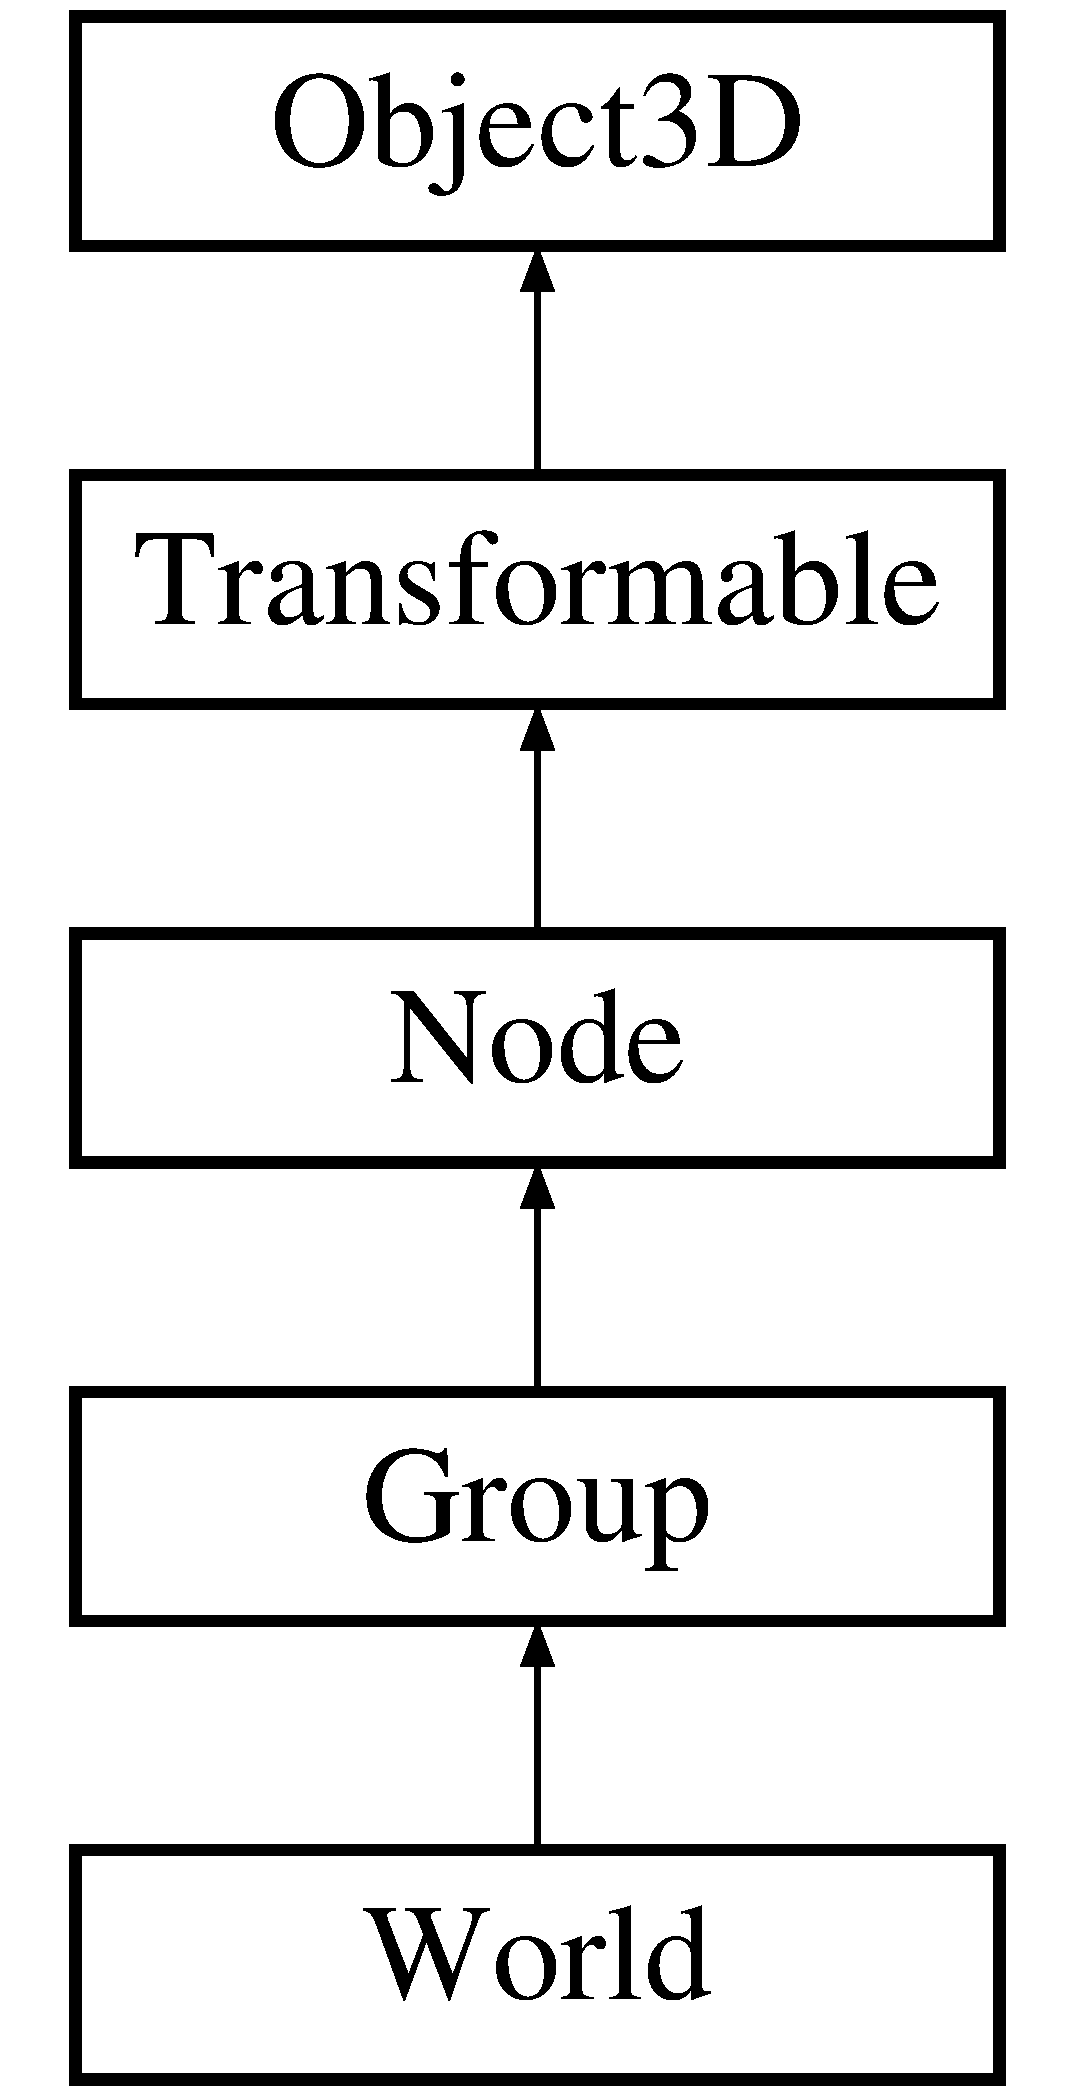
\includegraphics[height=5cm]{classm3g_1_1World}
\end{center}
\end{figure}
\subsection*{Public メソッド}
\begin{CompactItemize}
\item 
\hyperlink{classm3g_1_1World_75e827b8787e735882f60c266d58e02e}{World} ()
\item 
virtual \hyperlink{classm3g_1_1World_bd170ded455f0b2273c1fe06da6ea0cb}{$\sim$World} ()
\item 
virtual int \hyperlink{classm3g_1_1World_8aad1ceab4c2a03609c8a42324ce484d}{animate} (int world\_\-time)
\item 
\hyperlink{classm3g_1_1Camera}{Camera} $\ast$ \hyperlink{classm3g_1_1World_812e01ec4fd0fd872b0ca5ea6a30b2f6}{getActiveCamera} () const 
\item 
\hyperlink{classm3g_1_1Background}{Background} $\ast$ \hyperlink{classm3g_1_1World_fb10ab7fd2ad14b7b1d49caf129670e0}{getBackground} () const 
\item 
void \hyperlink{classm3g_1_1World_dd9a82b335e8521592ad410c662a5cfd}{setActiveCamera} (\hyperlink{classm3g_1_1Camera}{Camera} $\ast$camera)
\item 
void \hyperlink{classm3g_1_1World_6193765c76d6dc0450f264918ebe7e1c}{setBackground} (\hyperlink{classm3g_1_1Background}{Background} $\ast$background)
\item 
virtual std::ostream \& \hyperlink{classm3g_1_1World_6fea17fa1532df3794f8cb39cb4f911f}{print} (std::ostream \&out) const 
\end{CompactItemize}
\subsection*{Protected メソッド}
\begin{CompactItemize}
\item 
virtual void \hyperlink{classm3g_1_1World_1efcb1973989d9963d5bd6d03065d389}{render} (int pass, int index=0) const 
\end{CompactItemize}
\subsection*{フレンド}
\begin{CompactItemize}
\item 
\hypertarget{classm3g_1_1World_8174d4c629550c1ee279571250236ef4}{
class \textbf{Graphics3D}}
\label{classm3g_1_1World_8174d4c629550c1ee279571250236ef4}

\end{CompactItemize}


\subsection{説明}
シーングラフを保持する最上位の特殊グループノード. 

\subsection{コンストラクタとデストラクタ}
\hypertarget{classm3g_1_1World_75e827b8787e735882f60c266d58e02e}{
\index{m3g::World@{m3g::World}!World@{World}}
\index{World@{World}!m3g::World@{m3g::World}}
\subsubsection[{World}]{\setlength{\rightskip}{0pt plus 5cm}{\bf World} ()}}
\label{classm3g_1_1World_75e827b8787e735882f60c266d58e02e}


デフォルト値のWorldオブジェクトの作成. \hypertarget{classm3g_1_1World_bd170ded455f0b2273c1fe06da6ea0cb}{
\index{m3g::World@{m3g::World}!$\sim$World@{$\sim$World}}
\index{$\sim$World@{$\sim$World}!m3g::World@{m3g::World}}
\subsubsection[{$\sim$World}]{\setlength{\rightskip}{0pt plus 5cm}$\sim${\bf World} ()\hspace{0.3cm}{\tt  \mbox{[}virtual\mbox{]}}}}
\label{classm3g_1_1World_bd170ded455f0b2273c1fe06da6ea0cb}


このオブジェクトを削除するデストラクタ. 

\subsection{関数}
\hypertarget{classm3g_1_1World_8aad1ceab4c2a03609c8a42324ce484d}{
\index{m3g::World@{m3g::World}!animate@{animate}}
\index{animate@{animate}!m3g::World@{m3g::World}}
\subsubsection[{animate}]{\setlength{\rightskip}{0pt plus 5cm}int animate (int {\em world\_\-time})\hspace{0.3cm}{\tt  \mbox{[}virtual\mbox{]}}}}
\label{classm3g_1_1World_8aad1ceab4c2a03609c8a42324ce484d}


このObject3D自身とここから到達できるObject3Dのアニメーテッドプロパティを更新する. 

\hyperlink{classm3g_1_1Group_8aad1ceab4c2a03609c8a42324ce484d}{Group}を再定義しています。\hypertarget{classm3g_1_1World_812e01ec4fd0fd872b0ca5ea6a30b2f6}{
\index{m3g::World@{m3g::World}!getActiveCamera@{getActiveCamera}}
\index{getActiveCamera@{getActiveCamera}!m3g::World@{m3g::World}}
\subsubsection[{getActiveCamera}]{\setlength{\rightskip}{0pt plus 5cm}{\bf Camera} $\ast$ getActiveCamera () const}}
\label{classm3g_1_1World_812e01ec4fd0fd872b0ca5ea6a30b2f6}


カレントのアクティブカメラの取得. \hypertarget{classm3g_1_1World_fb10ab7fd2ad14b7b1d49caf129670e0}{
\index{m3g::World@{m3g::World}!getBackground@{getBackground}}
\index{getBackground@{getBackground}!m3g::World@{m3g::World}}
\subsubsection[{getBackground}]{\setlength{\rightskip}{0pt plus 5cm}{\bf Background} $\ast$ getBackground () const}}
\label{classm3g_1_1World_fb10ab7fd2ad14b7b1d49caf129670e0}


このWorldのバックグラウンド設定の取得. \hypertarget{classm3g_1_1World_6fea17fa1532df3794f8cb39cb4f911f}{
\index{m3g::World@{m3g::World}!print@{print}}
\index{print@{print}!m3g::World@{m3g::World}}
\subsubsection[{print}]{\setlength{\rightskip}{0pt plus 5cm}std::ostream \& print (std::ostream \& {\em out}) const\hspace{0.3cm}{\tt  \mbox{[}virtual\mbox{]}}}}
\label{classm3g_1_1World_6fea17fa1532df3794f8cb39cb4f911f}


このWorldクラスの情報を表示する。デバッグ用. 

\hyperlink{classm3g_1_1Group_6fea17fa1532df3794f8cb39cb4f911f}{Group}を再定義しています。\hypertarget{classm3g_1_1World_1efcb1973989d9963d5bd6d03065d389}{
\index{m3g::World@{m3g::World}!render@{render}}
\index{render@{render}!m3g::World@{m3g::World}}
\subsubsection[{render}]{\setlength{\rightskip}{0pt plus 5cm}void render (int {\em pass}, \/  int {\em index} = {\tt 0}) const\hspace{0.3cm}{\tt  \mbox{[}protected, virtual\mbox{]}}}}
\label{classm3g_1_1World_1efcb1973989d9963d5bd6d03065d389}


このノードをレンダリングする内部使用の関数.

Note: \hyperlink{classm3g_1_1World}{World} should be rendered via all rendering pass. pass=0: render background and camera. pass=1: render lights. pass=2: render objets. 

\hyperlink{classm3g_1_1Group_1efcb1973989d9963d5bd6d03065d389}{Group}を再定義しています。\hypertarget{classm3g_1_1World_dd9a82b335e8521592ad410c662a5cfd}{
\index{m3g::World@{m3g::World}!setActiveCamera@{setActiveCamera}}
\index{setActiveCamera@{setActiveCamera}!m3g::World@{m3g::World}}
\subsubsection[{setActiveCamera}]{\setlength{\rightskip}{0pt plus 5cm}void setActiveCamera ({\bf Camera} $\ast$ {\em camera})}}
\label{classm3g_1_1World_dd9a82b335e8521592ad410c662a5cfd}


このWorldをレンダリングするときに使われるカメラの設定. \hypertarget{classm3g_1_1World_6193765c76d6dc0450f264918ebe7e1c}{
\index{m3g::World@{m3g::World}!setBackground@{setBackground}}
\index{setBackground@{setBackground}!m3g::World@{m3g::World}}
\subsubsection[{setBackground}]{\setlength{\rightskip}{0pt plus 5cm}void setBackground ({\bf Background} $\ast$ {\em background})}}
\label{classm3g_1_1World_6193765c76d6dc0450f264918ebe7e1c}


このWorldのバックグラウンドオブジェ区の設定. 

このクラスの説明は次のファイルから生成されました:\begin{CompactItemize}
\item 
/work/desktop-m3g/src/World.hpp\item 
/work/desktop-m3g/src/World.cpp\end{CompactItemize}

\printindex
\end{document}
